% Options for packages loaded elsewhere
\PassOptionsToPackage{unicode}{hyperref}
\PassOptionsToPackage{hyphens}{url}
\PassOptionsToPackage{dvipsnames,svgnames,x11names}{xcolor}
%
\documentclass[
  letterpaper,
  DIV=11,
  numbers=noendperiod]{scrreprt}

\usepackage{amsmath,amssymb}
\usepackage{iftex}
\ifPDFTeX
  \usepackage[T1]{fontenc}
  \usepackage[utf8]{inputenc}
  \usepackage{textcomp} % provide euro and other symbols
\else % if luatex or xetex
  \usepackage{unicode-math}
  \defaultfontfeatures{Scale=MatchLowercase}
  \defaultfontfeatures[\rmfamily]{Ligatures=TeX,Scale=1}
\fi
\usepackage{lmodern}
\ifPDFTeX\else  
    % xetex/luatex font selection
\fi
% Use upquote if available, for straight quotes in verbatim environments
\IfFileExists{upquote.sty}{\usepackage{upquote}}{}
\IfFileExists{microtype.sty}{% use microtype if available
  \usepackage[]{microtype}
  \UseMicrotypeSet[protrusion]{basicmath} % disable protrusion for tt fonts
}{}
\makeatletter
\@ifundefined{KOMAClassName}{% if non-KOMA class
  \IfFileExists{parskip.sty}{%
    \usepackage{parskip}
  }{% else
    \setlength{\parindent}{0pt}
    \setlength{\parskip}{6pt plus 2pt minus 1pt}}
}{% if KOMA class
  \KOMAoptions{parskip=half}}
\makeatother
\usepackage{xcolor}
\setlength{\emergencystretch}{3em} % prevent overfull lines
\setcounter{secnumdepth}{5}
% Make \paragraph and \subparagraph free-standing
\ifx\paragraph\undefined\else
  \let\oldparagraph\paragraph
  \renewcommand{\paragraph}[1]{\oldparagraph{#1}\mbox{}}
\fi
\ifx\subparagraph\undefined\else
  \let\oldsubparagraph\subparagraph
  \renewcommand{\subparagraph}[1]{\oldsubparagraph{#1}\mbox{}}
\fi

\usepackage{color}
\usepackage{fancyvrb}
\newcommand{\VerbBar}{|}
\newcommand{\VERB}{\Verb[commandchars=\\\{\}]}
\DefineVerbatimEnvironment{Highlighting}{Verbatim}{commandchars=\\\{\}}
% Add ',fontsize=\small' for more characters per line
\usepackage{framed}
\definecolor{shadecolor}{RGB}{241,243,245}
\newenvironment{Shaded}{\begin{snugshade}}{\end{snugshade}}
\newcommand{\AlertTok}[1]{\textcolor[rgb]{0.68,0.00,0.00}{#1}}
\newcommand{\AnnotationTok}[1]{\textcolor[rgb]{0.37,0.37,0.37}{#1}}
\newcommand{\AttributeTok}[1]{\textcolor[rgb]{0.40,0.45,0.13}{#1}}
\newcommand{\BaseNTok}[1]{\textcolor[rgb]{0.68,0.00,0.00}{#1}}
\newcommand{\BuiltInTok}[1]{\textcolor[rgb]{0.00,0.23,0.31}{#1}}
\newcommand{\CharTok}[1]{\textcolor[rgb]{0.13,0.47,0.30}{#1}}
\newcommand{\CommentTok}[1]{\textcolor[rgb]{0.37,0.37,0.37}{#1}}
\newcommand{\CommentVarTok}[1]{\textcolor[rgb]{0.37,0.37,0.37}{\textit{#1}}}
\newcommand{\ConstantTok}[1]{\textcolor[rgb]{0.56,0.35,0.01}{#1}}
\newcommand{\ControlFlowTok}[1]{\textcolor[rgb]{0.00,0.23,0.31}{#1}}
\newcommand{\DataTypeTok}[1]{\textcolor[rgb]{0.68,0.00,0.00}{#1}}
\newcommand{\DecValTok}[1]{\textcolor[rgb]{0.68,0.00,0.00}{#1}}
\newcommand{\DocumentationTok}[1]{\textcolor[rgb]{0.37,0.37,0.37}{\textit{#1}}}
\newcommand{\ErrorTok}[1]{\textcolor[rgb]{0.68,0.00,0.00}{#1}}
\newcommand{\ExtensionTok}[1]{\textcolor[rgb]{0.00,0.23,0.31}{#1}}
\newcommand{\FloatTok}[1]{\textcolor[rgb]{0.68,0.00,0.00}{#1}}
\newcommand{\FunctionTok}[1]{\textcolor[rgb]{0.28,0.35,0.67}{#1}}
\newcommand{\ImportTok}[1]{\textcolor[rgb]{0.00,0.46,0.62}{#1}}
\newcommand{\InformationTok}[1]{\textcolor[rgb]{0.37,0.37,0.37}{#1}}
\newcommand{\KeywordTok}[1]{\textcolor[rgb]{0.00,0.23,0.31}{#1}}
\newcommand{\NormalTok}[1]{\textcolor[rgb]{0.00,0.23,0.31}{#1}}
\newcommand{\OperatorTok}[1]{\textcolor[rgb]{0.37,0.37,0.37}{#1}}
\newcommand{\OtherTok}[1]{\textcolor[rgb]{0.00,0.23,0.31}{#1}}
\newcommand{\PreprocessorTok}[1]{\textcolor[rgb]{0.68,0.00,0.00}{#1}}
\newcommand{\RegionMarkerTok}[1]{\textcolor[rgb]{0.00,0.23,0.31}{#1}}
\newcommand{\SpecialCharTok}[1]{\textcolor[rgb]{0.37,0.37,0.37}{#1}}
\newcommand{\SpecialStringTok}[1]{\textcolor[rgb]{0.13,0.47,0.30}{#1}}
\newcommand{\StringTok}[1]{\textcolor[rgb]{0.13,0.47,0.30}{#1}}
\newcommand{\VariableTok}[1]{\textcolor[rgb]{0.07,0.07,0.07}{#1}}
\newcommand{\VerbatimStringTok}[1]{\textcolor[rgb]{0.13,0.47,0.30}{#1}}
\newcommand{\WarningTok}[1]{\textcolor[rgb]{0.37,0.37,0.37}{\textit{#1}}}

\providecommand{\tightlist}{%
  \setlength{\itemsep}{0pt}\setlength{\parskip}{0pt}}\usepackage{longtable,booktabs,array}
\usepackage{calc} % for calculating minipage widths
% Correct order of tables after \paragraph or \subparagraph
\usepackage{etoolbox}
\makeatletter
\patchcmd\longtable{\par}{\if@noskipsec\mbox{}\fi\par}{}{}
\makeatother
% Allow footnotes in longtable head/foot
\IfFileExists{footnotehyper.sty}{\usepackage{footnotehyper}}{\usepackage{footnote}}
\makesavenoteenv{longtable}
\usepackage{graphicx}
\makeatletter
\def\maxwidth{\ifdim\Gin@nat@width>\linewidth\linewidth\else\Gin@nat@width\fi}
\def\maxheight{\ifdim\Gin@nat@height>\textheight\textheight\else\Gin@nat@height\fi}
\makeatother
% Scale images if necessary, so that they will not overflow the page
% margins by default, and it is still possible to overwrite the defaults
% using explicit options in \includegraphics[width, height, ...]{}
\setkeys{Gin}{width=\maxwidth,height=\maxheight,keepaspectratio}
% Set default figure placement to htbp
\makeatletter
\def\fps@figure{htbp}
\makeatother
% definitions for citeproc citations
\NewDocumentCommand\citeproctext{}{}
\NewDocumentCommand\citeproc{mm}{%
  \begingroup\def\citeproctext{#2}\cite{#1}\endgroup}
\makeatletter
 % allow citations to break across lines
 \let\@cite@ofmt\@firstofone
 % avoid brackets around text for \cite:
 \def\@biblabel#1{}
 \def\@cite#1#2{{#1\if@tempswa , #2\fi}}
\makeatother
\newlength{\cslhangindent}
\setlength{\cslhangindent}{1.5em}
\newlength{\csllabelwidth}
\setlength{\csllabelwidth}{3em}
\newenvironment{CSLReferences}[2] % #1 hanging-indent, #2 entry-spacing
 {\begin{list}{}{%
  \setlength{\itemindent}{0pt}
  \setlength{\leftmargin}{0pt}
  \setlength{\parsep}{0pt}
  % turn on hanging indent if param 1 is 1
  \ifodd #1
   \setlength{\leftmargin}{\cslhangindent}
   \setlength{\itemindent}{-1\cslhangindent}
  \fi
  % set entry spacing
  \setlength{\itemsep}{#2\baselineskip}}}
 {\end{list}}
\usepackage{calc}
\newcommand{\CSLBlock}[1]{\hfill\break\parbox[t]{\linewidth}{\strut\ignorespaces#1\strut}}
\newcommand{\CSLLeftMargin}[1]{\parbox[t]{\csllabelwidth}{\strut#1\strut}}
\newcommand{\CSLRightInline}[1]{\parbox[t]{\linewidth - \csllabelwidth}{\strut#1\strut}}
\newcommand{\CSLIndent}[1]{\hspace{\cslhangindent}#1}

\KOMAoption{captions}{tableheading}
\makeatletter
\@ifpackageloaded{bookmark}{}{\usepackage{bookmark}}
\makeatother
\makeatletter
\@ifpackageloaded{caption}{}{\usepackage{caption}}
\AtBeginDocument{%
\ifdefined\contentsname
  \renewcommand*\contentsname{Table of contents}
\else
  \newcommand\contentsname{Table of contents}
\fi
\ifdefined\listfigurename
  \renewcommand*\listfigurename{List of Figures}
\else
  \newcommand\listfigurename{List of Figures}
\fi
\ifdefined\listtablename
  \renewcommand*\listtablename{List of Tables}
\else
  \newcommand\listtablename{List of Tables}
\fi
\ifdefined\figurename
  \renewcommand*\figurename{Figure}
\else
  \newcommand\figurename{Figure}
\fi
\ifdefined\tablename
  \renewcommand*\tablename{Table}
\else
  \newcommand\tablename{Table}
\fi
}
\@ifpackageloaded{float}{}{\usepackage{float}}
\floatstyle{ruled}
\@ifundefined{c@chapter}{\newfloat{codelisting}{h}{lop}}{\newfloat{codelisting}{h}{lop}[chapter]}
\floatname{codelisting}{Listing}
\newcommand*\listoflistings{\listof{codelisting}{List of Listings}}
\makeatother
\makeatletter
\makeatother
\makeatletter
\@ifpackageloaded{caption}{}{\usepackage{caption}}
\@ifpackageloaded{subcaption}{}{\usepackage{subcaption}}
\makeatother
\ifLuaTeX
  \usepackage{selnolig}  % disable illegal ligatures
\fi
\usepackage{bookmark}

\IfFileExists{xurl.sty}{\usepackage{xurl}}{} % add URL line breaks if available
\urlstyle{same} % disable monospaced font for URLs
\hypersetup{
  pdftitle={Probability And Business Statistics},
  pdfauthor={Pamela Schlosser},
  colorlinks=true,
  linkcolor={blue},
  filecolor={Maroon},
  citecolor={Blue},
  urlcolor={Blue},
  pdfcreator={LaTeX via pandoc}}

\title{Probability And Business Statistics}
\author{Pamela Schlosser}
\date{2024-05-17}

\begin{document}
\maketitle

\renewcommand*\contentsname{Table of contents}
{
\hypersetup{linkcolor=}
\setcounter{tocdepth}{2}
\tableofcontents
}
\bookmarksetup{startatroot}

\chapter{Installing R and R Studio}\label{installing-r-and-r-studio}

\section{Installing R on Windows}\label{installing-r-on-windows}

\begin{itemize}
\tightlist
\item
  Open an internet browser and go to https://www.r-project.org/.
\item
  Click CRAN hyperlink underneath Download on the left.
\item
  Select a CRAN location (a mirror site) and click the corresponding
  link. I selected O-cloud. This brings you to the following link:
  https://cloud.r-project.org/
\item
  Click on the ``Download R for Windows'' link at the top of the page if
  you have a Windows computer.\\
\item
  Click on the ``install R for the first time'' link at the top of the
  page.
\item
  Click ``Download R for Windows'' and save the executable file
  somewhere on your computer.
\item
  Run the .exe file
\item
  Accept all defaults and follow the installation instructions
\item
  Now that R is installed, you need to download and install RStudio.
\end{itemize}

\section{Installing R on a Mac}\label{installing-r-on-a-mac}

\begin{itemize}
\tightlist
\item
  Open an internet browser and go to https://www.r-project.org/.
\item
  Click CRAN hyperlink underneath Download on the left.
\item
  Select a CRAN location (a mirror site) and click the corresponding
  link. I selected O-cloud. This brings you to the following link:
  https://cloud.r-project.org/
\item
  Click on the ``Download R for (Mac) OS X'' link at the top of the
  page.
\item
  Click on the file containing the latest version of R under ``Files.''
\item
  Save the .pkg file, double-click it to open, and follow the
  installation instructions.
\item
  Accept the license agreement and all subsequent defaults
\item
  When the installation completes, click Close.
\item
  Now that R is installed, you need to download and install RStudio.
\end{itemize}

\section{Downloading RStudio For Mac or
PC}\label{downloading-rstudio-for-mac-or-pc}

\begin{itemize}
\tightlist
\item
  Go to the following URL:
  https://www.rstudio.com/products/rstudio/download/
\item
  Click the Download button for Install RStudio.
\item
  It should recognize your operating system. If you see different an
  Installers for Supported Platforms section, click the version that is
  appropriate for your operating system. When the download is complete,
  run the install program, accepting all defaults.
\item
  Note, RStudio might conflict with some Mac antivirus programs. Ensure
  your antivirus is not blocking it from installing. Only worry about
  this if you have difficulty installing the program.
\end{itemize}

\begin{figure}[H]

{\centering 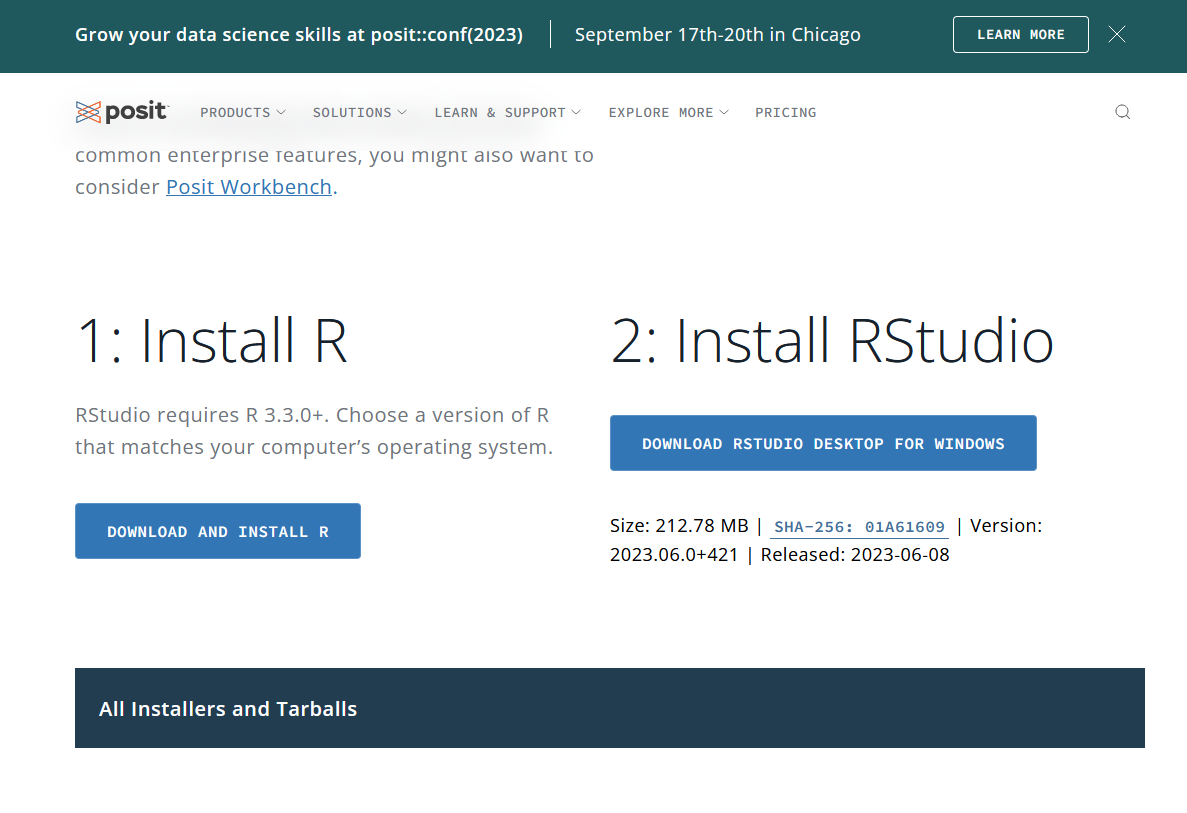
\includegraphics{Pictures/Ch0/RStudio.png}

}

\caption{RStudio}

\end{figure}%

\bookmarksetup{startatroot}

\chapter{Take Your First Look at R}\label{take-your-first-look-at-r}

\begin{itemize}
\tightlist
\item
  On the right, two windows, each with tabs

  \begin{itemize}
  \tightlist
  \item
    There are many ways to customize the look of RStudio for
    accessibility purposes with a couple being the following:

    \begin{itemize}
    \tightlist
    \item
      You can resize the windows using the splitters.
    \item
      You can maximize/restore the windows within the left/right panels
      using the familiar Windows controls in the upper-right of each
      window.
    \end{itemize}
  \end{itemize}
\item
  On the left, the Console Window reproduces the R environment.

  \begin{itemize}
  \tightlist
  \item
    Observe the command line with the \(>\) symbol.
  \end{itemize}
\end{itemize}

\begin{figure}[H]

{\centering 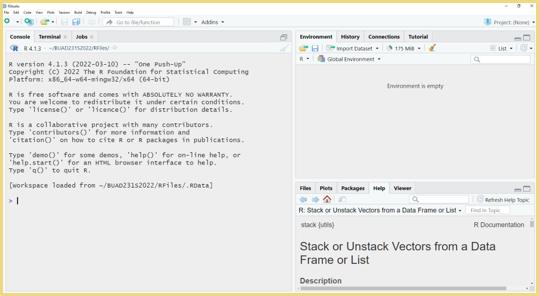
\includegraphics{Pictures/Ch0/Console.png}

}

\caption{Console}

\end{figure}%

\bookmarksetup{startatroot}

\chapter{Creating a Project for Our
Class}\label{creating-a-project-for-our-class}

\begin{itemize}
\tightlist
\item
  The RStudio project file is a file that sits in the root directory,
  with the extension .Rproj. When your RStudio session is running
  through the project file (.Rproj), the current working directory
  points to the root folder where that .Rproj file is saved.
\item
  Open up R Studio and Let's Take a look around.
\item
  Start by creating a project for our class. Projects are great because
  they aid in your organization technique.
\item
  You will find that some professors are not insistent on making a
  project for their class, but it is helpful to still do to organize
  your materials. You will have a lot of code in this class, so it is
  good practice to keep everything organized!
\item
  To create a project click
  \(File > New Project - New Directory > New Project\) and save your
  project to a place on your computer (not the cloud).
\end{itemize}

\begin{figure}[H]

{\centering 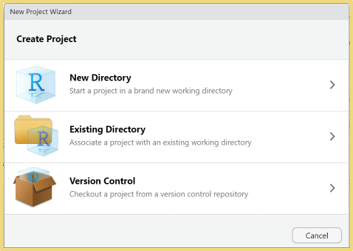
\includegraphics{Pictures/Ch0/CreateProject.png}

}

\caption{CreateProject}

\end{figure}%%
\begin{figure}[H]

{\centering 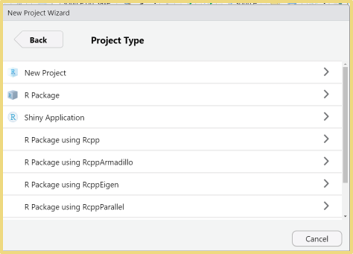
\includegraphics{Pictures/Ch0/Project.png}

}

\caption{Creating a New Project}

\end{figure}%

\bookmarksetup{startatroot}

\chapter{R Script files
(MyFirstRscript.R)}\label{r-script-files-myfirstrscript.r}

\begin{itemize}
\tightlist
\item
  Entering and running code at the R command line is effective and
  simple. However, each time you want to execute a set of commands, you
  have to re-enter them at the command line. Nothing saves for later.
\item
  Complex commands are particularly difficult causing you to re-entering
  the code to fix any errors typographical or otherwise. Fortunately,
  you can make a .R script file to solve this issue.
\item
  A .R script is simply a text file containing a set of commands and
  comments. The script can be saved and used later to rerun the code.
  The script can also be documented with comments and edited again and
  again to suit your needs.\\
\item
  Create your first R Script file within your Project for testing
  purposes.

  \begin{itemize}
  \tightlist
  \item
    Go to File \textgreater{} New File \textgreater{} R Script
  \item
    Save this file as MyFirstRscript.R in your project folder you just
    made. You should see this new file under Files like mine is in the
    bottom right panel. As we create new files, continue to save them
    into your project folder.
  \end{itemize}
\item
  On the .R file presented to the left, comments are added as denoted by
  the hashtag which you can type or push ctrl + shift + c.~
\item
  If you type in your console, it will not save it for later. However,
  if you save code in this R Script file, you can open your file at a
  later date to rerun your code. Also, as we move through the class,
  feel free to document all your notes in your .R file via \# called
  comments. More on comments later.
\end{itemize}

\begin{figure}[H]

{\centering 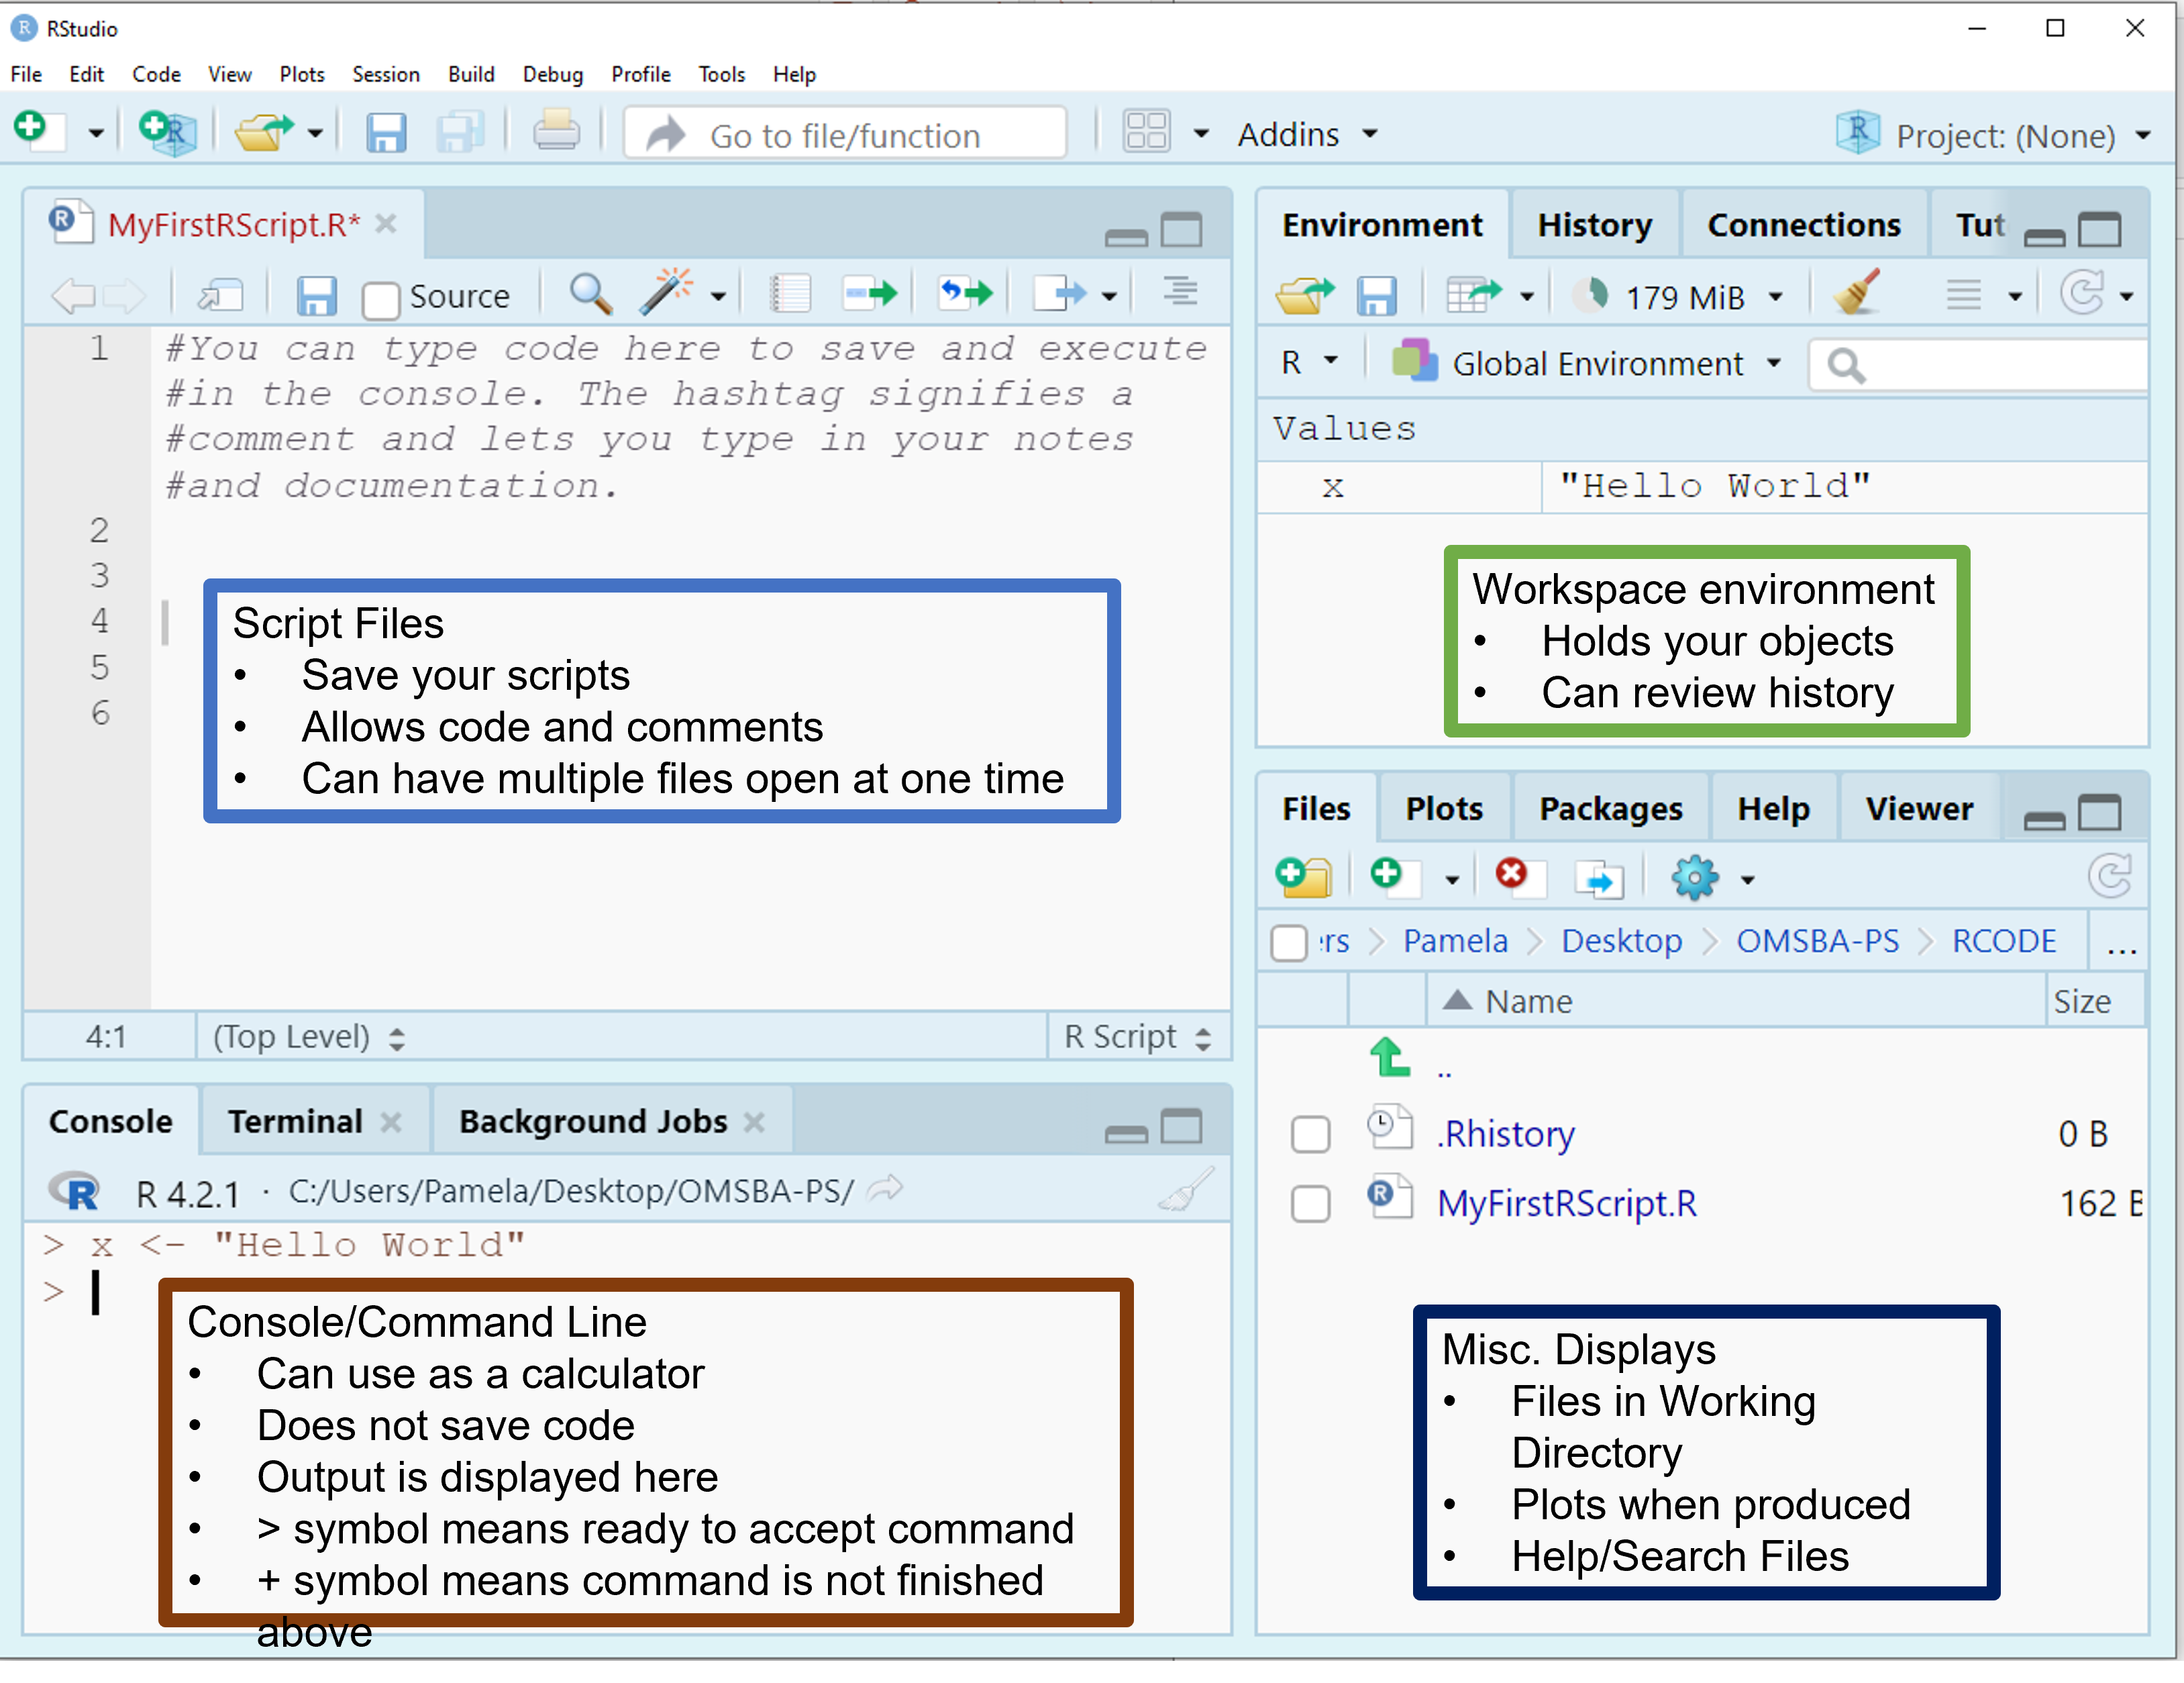
\includegraphics{Pictures/Ch0/MyFirstScript.png}

}

\caption{Screenshot of MyFirstScript.R}

\end{figure}%

\bookmarksetup{startatroot}

\chapter{Using R More Effectively}\label{using-r-more-effectively}

\section{Setting Options to Your
Liking}\label{setting-options-to-your-liking}

\begin{itemize}
\tightlist
\item
  You have many options to customize R Studio.
\item
  Go to Tools \textgreater{} Global Options to see the list of options
  for you to customize.
\item
  A few are listed below.

  \begin{itemize}
  \tightlist
  \item
    You can set your general information including your default working
    directory (when not in a project).
  \item
    You can customize the appearance to a theme that accommodates your
    learning style and visual preferences.
  \item
    You can turn on a spell check.
  \end{itemize}
\end{itemize}

\begin{figure}[H]

{\centering 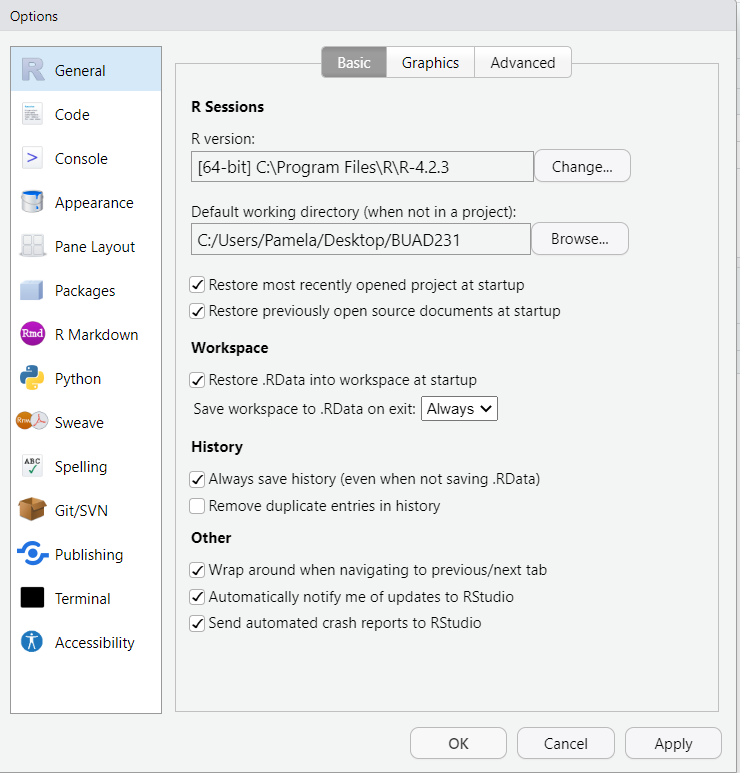
\includegraphics{Pictures/Ch0/Options.png}

}

\caption{Tools \textgreater{} Global Options.R}

\end{figure}%

\section{Quick Keys in R}\label{quick-keys-in-r}

\begin{itemize}
\tightlist
\item
  There are a lot of quick keys in R to make you able to use it faster
  and more effectively. You may look over these and try on your own.
\end{itemize}

\begin{figure}[H]

{\centering 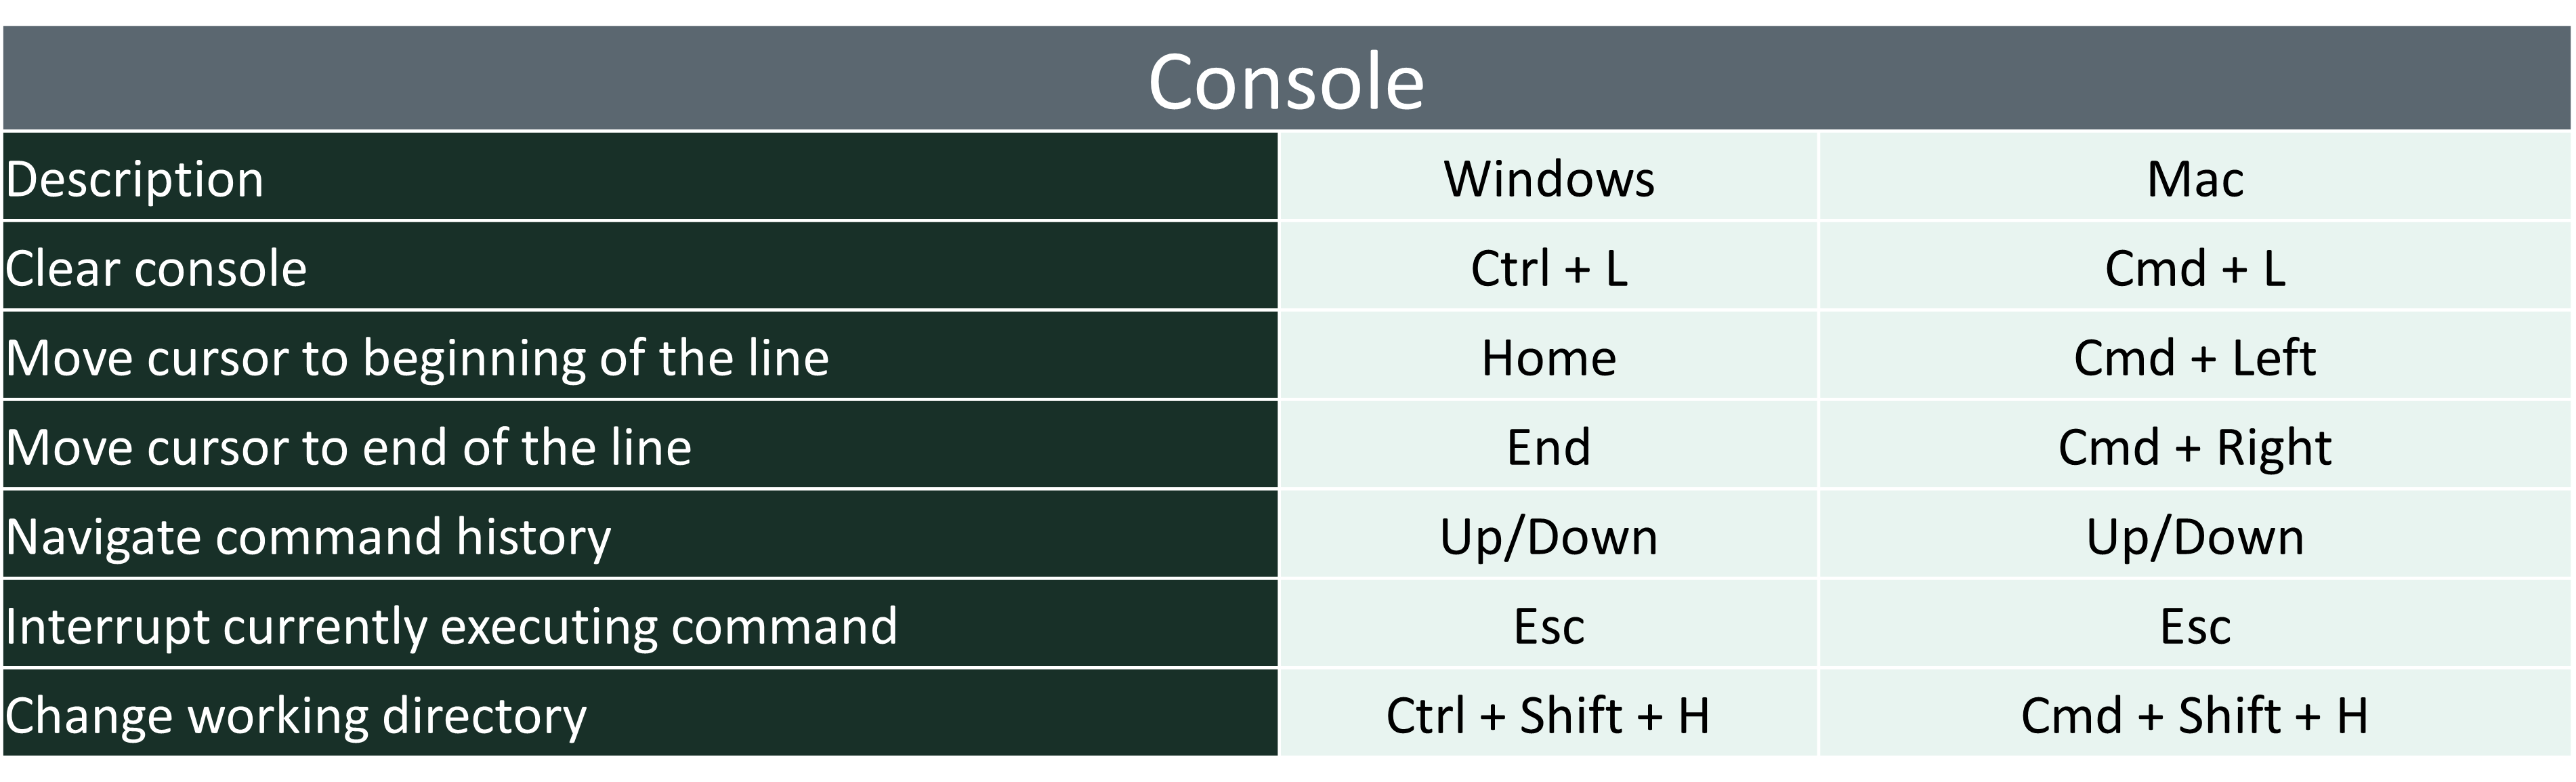
\includegraphics{Pictures/Ch0/QuickKeys1.png}

}

\caption{Console Quick Keys}

\end{figure}%%
\begin{figure}[H]

{\centering 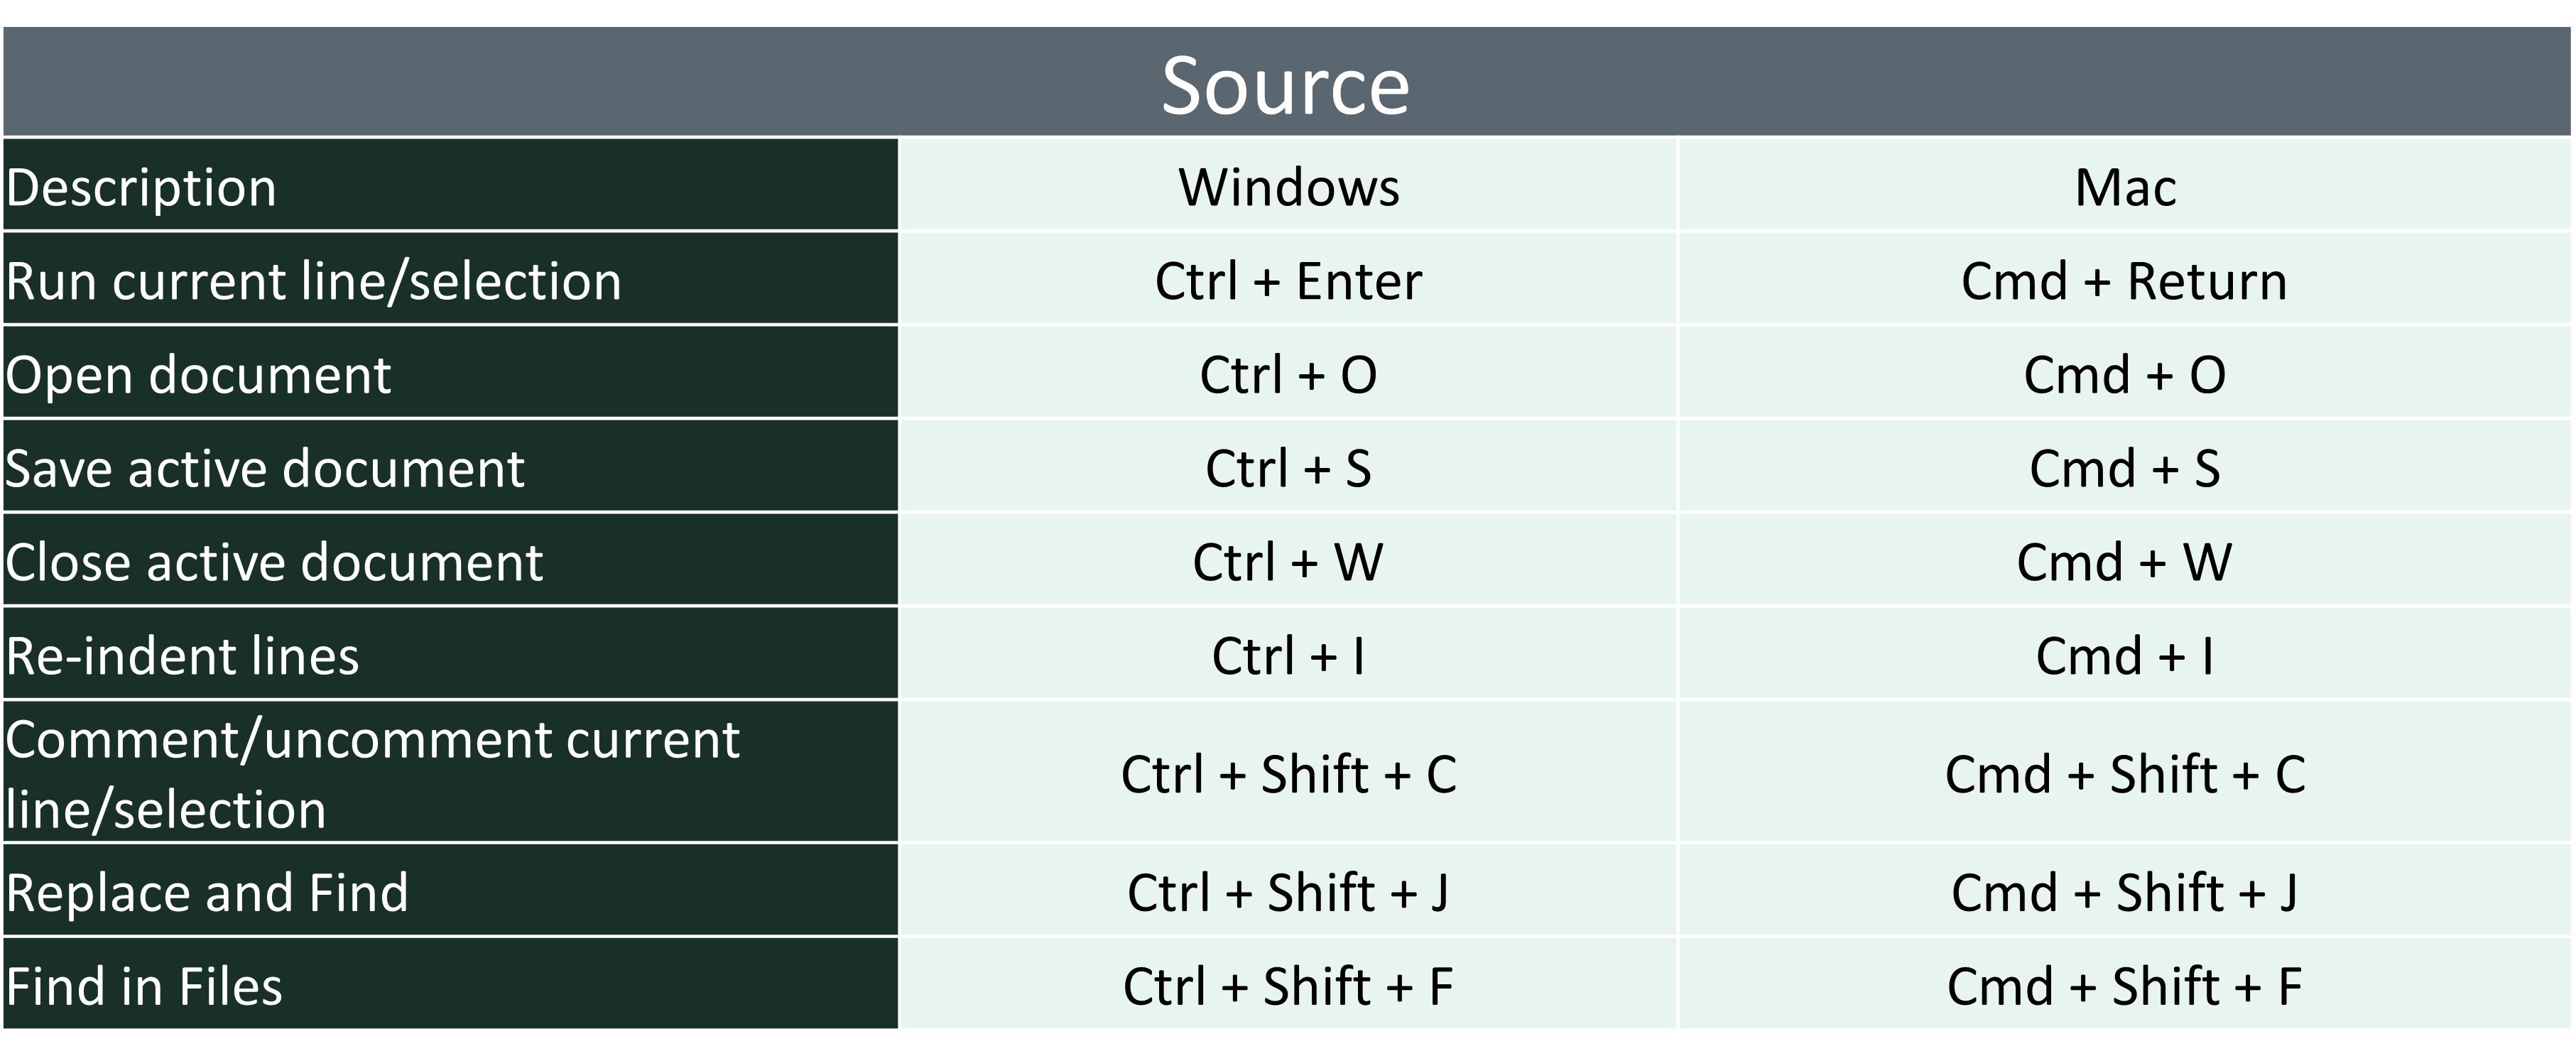
\includegraphics{Pictures/Ch0/QuickKeys2.png}

}

\caption{Source Quick Keys}

\end{figure}%%
\begin{figure}[H]

{\centering 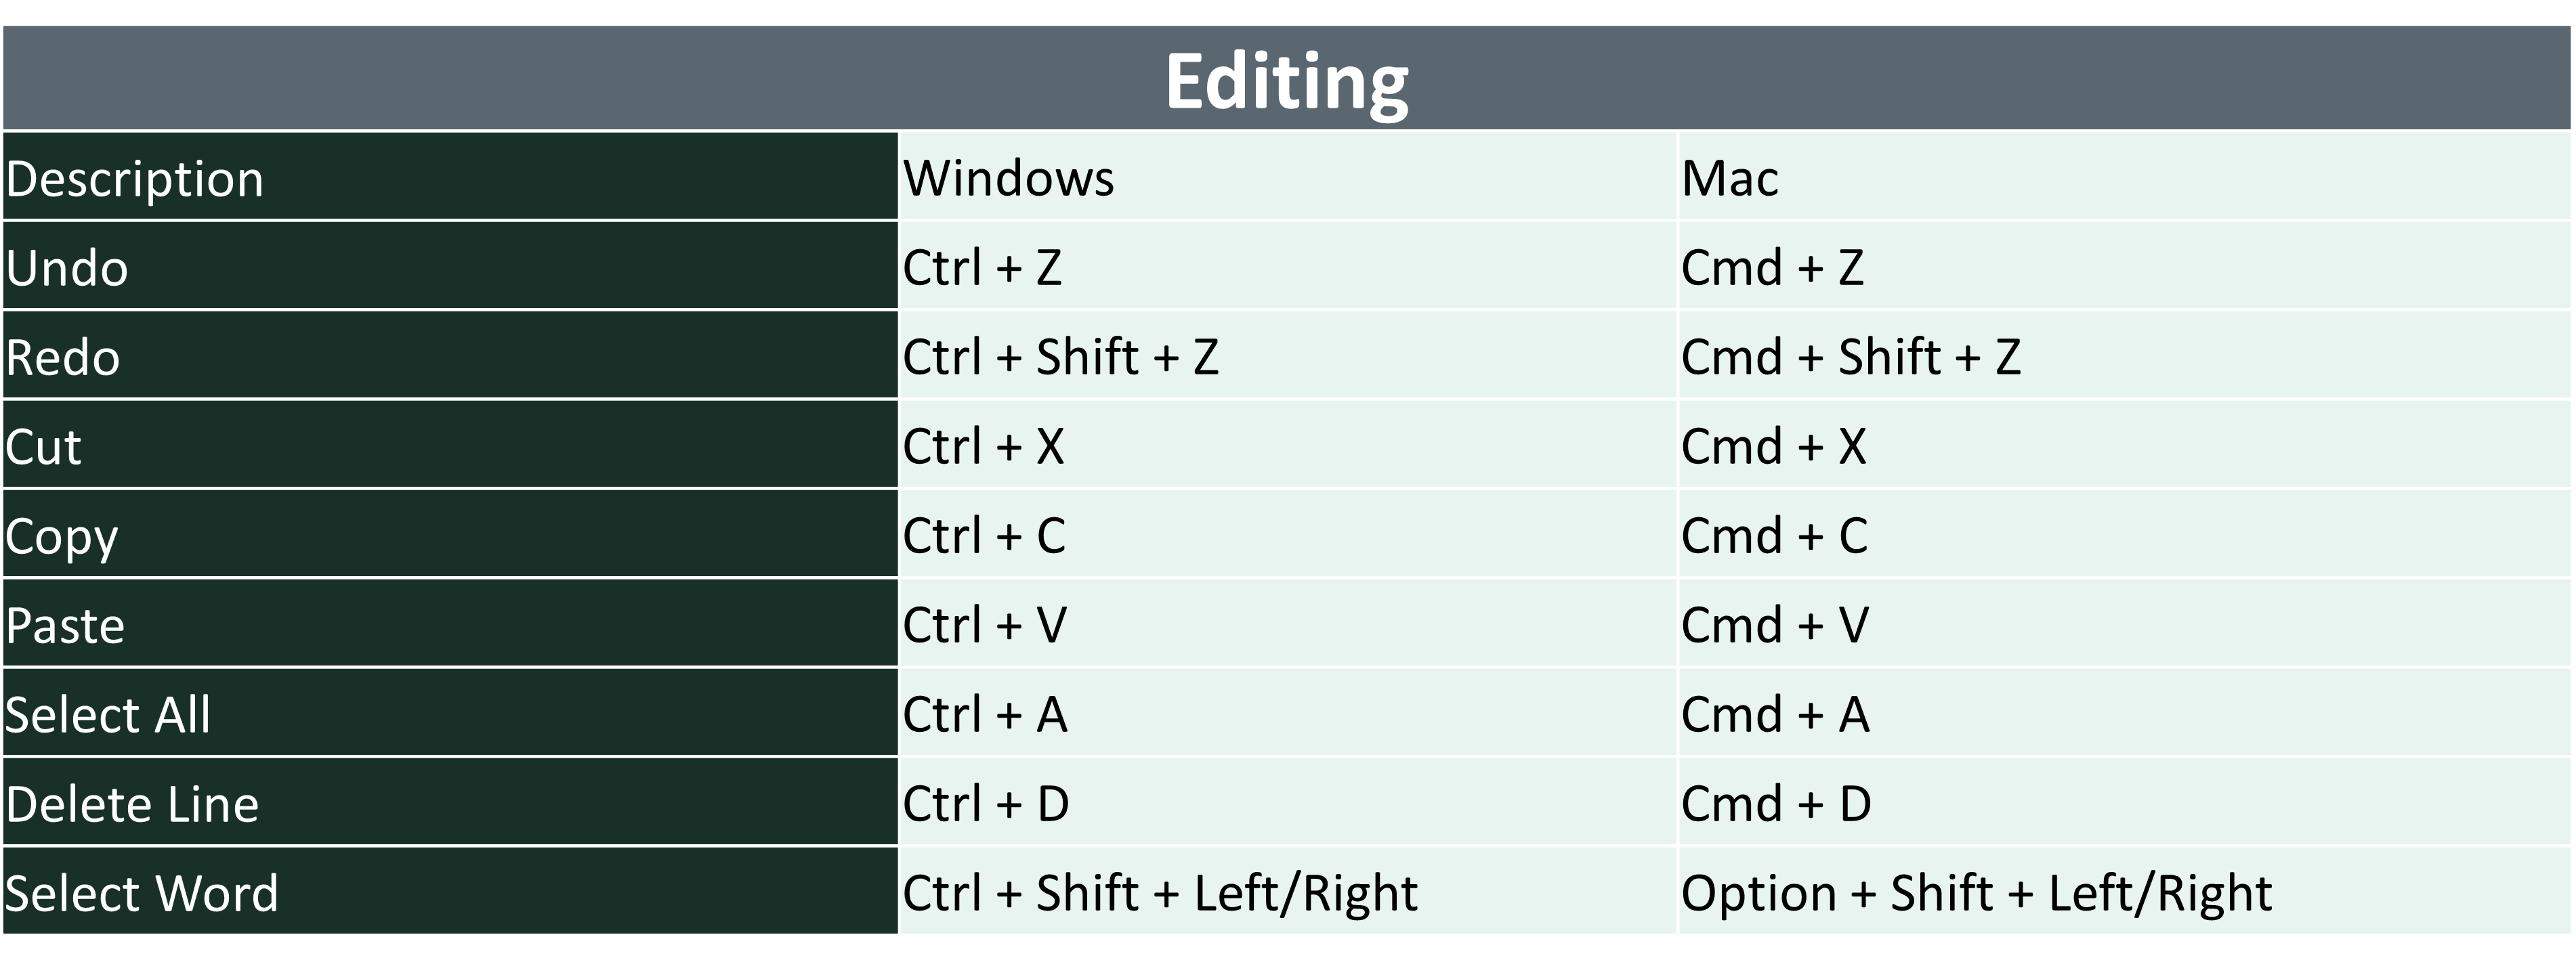
\includegraphics{Pictures/Ch0/QuickKeys3.png}

}

\caption{Editing Quick Keys}

\end{figure}%

\section{Getting Help in R}\label{getting-help-in-r}

\begin{itemize}
\tightlist
\item
  There are lots of ways to get help in R.
\item
  In R, use the help search box to find information on a function,
  parameter, or package.

  \begin{itemize}
  \tightlist
  \item
    ?mean
  \item
    help.search(`swirl')
  \item
    help(package = `MASS')
  \item
    ?install.packages
  \end{itemize}
\end{itemize}

\begin{figure}[H]

{\centering 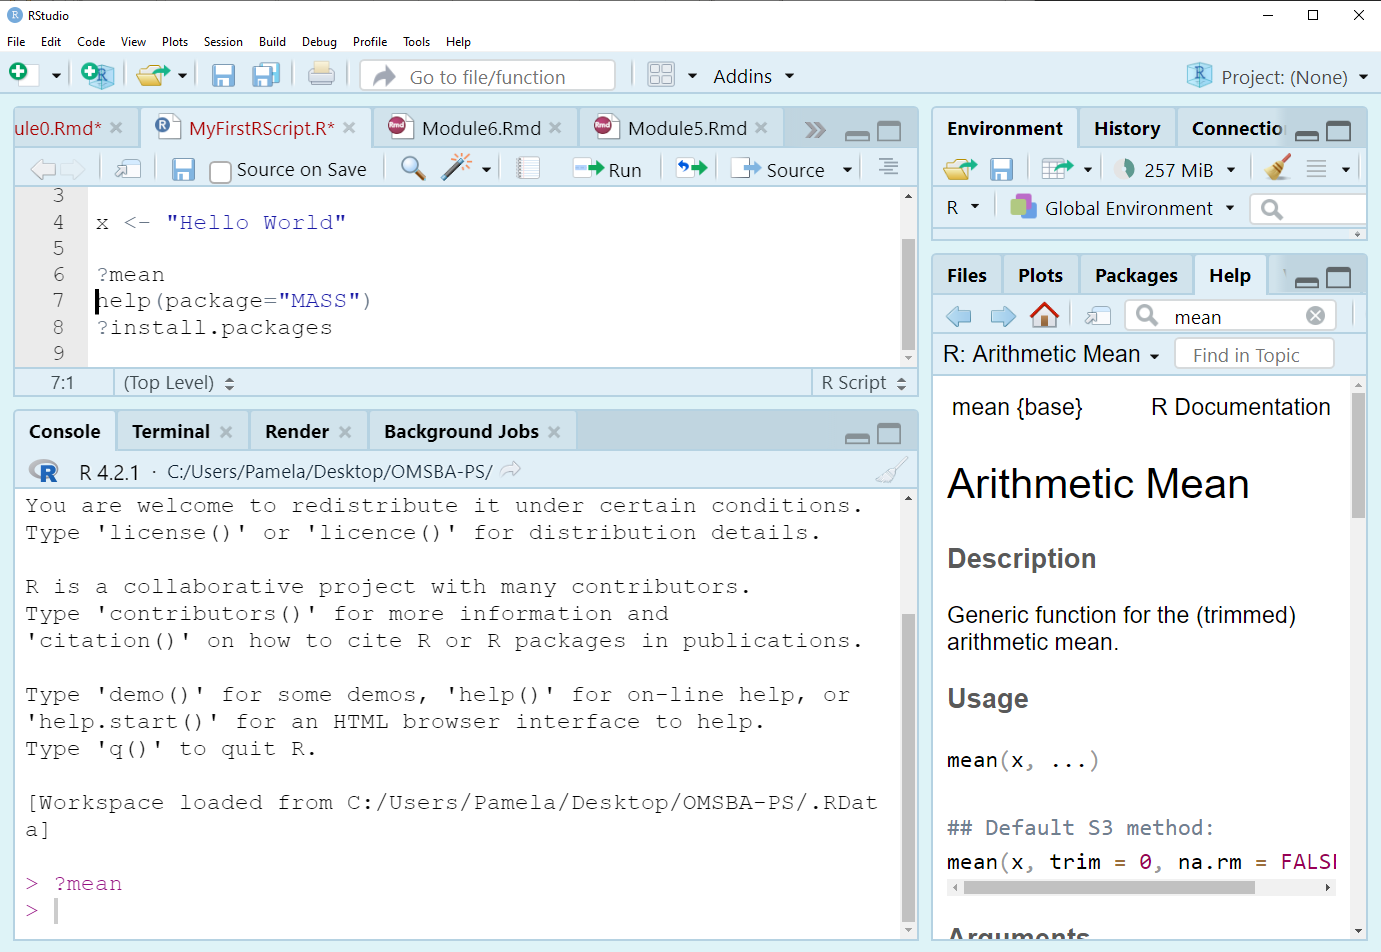
\includegraphics{Pictures/Ch0/Help.png}

}

\caption{Getting Help}

\end{figure}%

\begin{itemize}
\tightlist
\item
  You should try to look up the tapply command to see what it does.

  \begin{itemize}
  \tightlist
  \item
    Use ?tapply in your .R file to pull up tapply() command or type
    tapply in the Help box. * Formally, you should see that the command
    applies a function to each cell of a ragged array, that is to each
    (non-empty) group of values given by a unique combination of the
    levels of certain factors. This means that the command does some
    math calculation (mean, sum, etc.) on a continuous variable after
    dividing the data by group.
  \end{itemize}
\item
  The format is tapply(x, index, and fun), where x is a continuous
  variable, index is a grouping variable or factor, and fun is a
  function like mean.
\item
  More on that function later in Chapter 1.
\end{itemize}

\bookmarksetup{startatroot}

\chapter{Accessing Data Files for the
Book}\label{accessing-data-files-for-the-book}

\begin{itemize}
\tightlist
\item
  To download the data sets for the book, go to our Blackboard datasets
  page and download them to your computer
\item
  Once downloaded, unzip the file by right-clicking and selecting
  ``Extract All'', and then move the subfolder named data to your
  working directory.
\item
  In the example below, my project folder for the class is called
  BUAD231 and the subfolder that contains all the data files is called
  data. You can put your folder anywhere on the hard drive of your
  computer, but do not download it to places on the cloud like OneDrive.
\end{itemize}

\begin{figure}[H]

{\centering 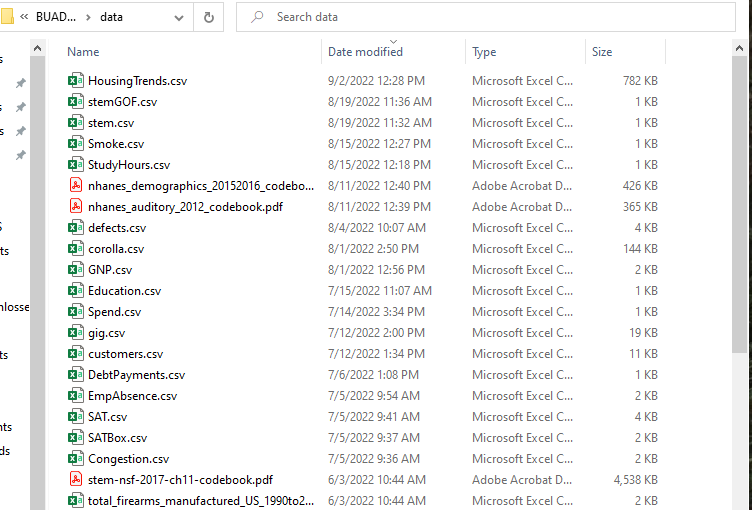
\includegraphics{Pictures/Ch0/BookFiles.png}

}

\caption{Saving Our Book Files Into a ``data'' Folder in Your Working
Directory}

\end{figure}%

\begin{itemize}
\tightlist
\item
  We will use a number of data files plus more for homework/projects, so
  be prepared to use these files throughout the class.
\end{itemize}

\bookmarksetup{startatroot}

\chapter{Summary}\label{summary}

\begin{itemize}
\tightlist
\item
  At the end of this section, you should have downloaded and browsed R
  in RStudio. You should have looked at the quick keys in R to make
  editing your R documents easier. You should set up a project folder
  for the course where you want to on your computer, and made your first
  .R script file located in that project folder. You should have tried a
  line of code or two as presented. Finally, you should have looked
  around the RStudio environment and found the help tab.
\end{itemize}

\bookmarksetup{startatroot}

\chapter{Introduction to R and
RStudio}\label{introduction-to-r-and-rstudio}

\begin{itemize}
\tightlist
\item
  The goal of this lesson is to introduce you to R and RStudio while
  teaching you how to perform data preparation using these tools. In
  this part, we will go over forming an understanding of statistics,
  learning about observations and variables, and being able to move
  around and get comfortable with R. I will also teach you how use and
  load data while also performing data preparation. This includes
  entering and loading information into R, identifying and treating
  missing values in a data set, and building a basic bar chart.
\end{itemize}

\begin{Shaded}
\begin{Highlighting}[]
\DocumentationTok{\#\#\#\#\#\#\#\#\#\#\#\#\#\#\#\#\#\#\#\#\#\#\#\#\#\#\#\#\#\#\#\#\#\#\#\#}
\CommentTok{\# Project name: Introduction to R and RStudio}
\CommentTok{\# Data used: mtcars from R, Insurance from the MASS library, gig.csv and gss2016.csv, }
\CommentTok{\# Libraries used: MASS, tidyverse, dplyr (part of tidyverse)}
\DocumentationTok{\#\#\#\#\#\#\#\#\#\#\#\#\#\#\#\#\#\#\#\#\#\#\#\#\#\#\#\#\#\#\#\#\#\#\#\#}
\end{Highlighting}
\end{Shaded}

\section{At a Glance}\label{at-a-glance}

\begin{itemize}
\tightlist
\item
  In order to succeed in this lesson, you will need to start by having
  both R and RStudio downloaded. Then, the only way to learn R is to use
  it in various ways and to practice as much as you can.
\item
  It is also important to note that this is a statistics class and that
  R is a statistical computing software. Because of that, we need to not
  only pay attention to what we are typing in, but understand why we are
  typing it in the ways suggested, and also how we could do it
  differently to get similar if not the same results. We also need to
  understand what important information we can pull from what we have
  done. Finally, to succeed in this section, we need to begin to
  understand how to clean data, which is a very important step for data
  analysts. Specifically, we learn how to count, sort, and handle
  missing data.
\end{itemize}

\section{Lesson Objectives}\label{lesson-objectives}

\begin{itemize}
\tightlist
\item
  Be Introduced to R and R Studio.
\item
  Set up R and R Studio.
\item
  Use basic Built-in Functions in R.
\item
  Enter and load data into R.
\item
  Identify and treat missing values.
\end{itemize}

\section{Consider While Reading}\label{consider-while-reading}

\begin{itemize}
\tightlist
\item
  This material is so important because it is likely the start of your R
  journey and will provide the groundwork for learning a modern approach
  to calculating statistics. R has a fairly steep learning curve, but,
  once you are over it, it becomes fairly easy to figure out new things.
  It is important to make connections to what we are doing and why we
  are doing it a certain way. There are rules to learning R, and you
  will get better with constant practice. Try to avoid just typing in
  code. Instead, determine why the code was typed the way it was and try
  to figure out all the other ways the code could also be typed to get
  the same answer. Practice, practice, practice!
\end{itemize}

\bookmarksetup{startatroot}

\chapter{What is Statistics?}\label{what-is-statistics}

\begin{itemize}
\tightlist
\item
  Statistics is the methodology of extracting useful information from a
  data set.
\item
  Numerical results are not very useful unless they are accompanied with
  clearly stated actionable business insights.
\item
  To do good statistical analysis, you must do the following:

  \begin{itemize}
  \tightlist
  \item
    Find the right data.
  \item
    Use the appropriate statistical tools.
  \item
    Clearly communicate the numerical information in written language.
  \end{itemize}
\item
  With knowledge of statistics:

  \begin{itemize}
  \tightlist
  \item
    Avoid risk of making uninformed decisions and costly mistakes.
  \item
    Differentiate between sound statistical conclusions and questionable
    conclusions.
  \end{itemize}
\item
  Data and analytics capabilities have made a leap forward.

  \begin{itemize}
  \tightlist
  \item
    Growing availability of vast amounts of data.
  \item
    Improved computational power.
  \item
    Development of sophisticated algorithms.
  \end{itemize}
\end{itemize}

\section{Two Main Branches of
Statistics}\label{two-main-branches-of-statistics}

\begin{itemize}
\tightlist
\item
  Descriptive Statistics - collecting, organizing, and presenting the
  data.
\item
  Inferential Statistics - drawing conclusions about a population based
  on sample data from that population.

  \begin{itemize}
  \tightlist
  \item
    A population consists of all items of interest.
  \item
    A sample is a subset of the population.
  \item
    A sample statistic is calculated from the sample data and is used to
    make inferences about the population parameter.
  \end{itemize}
\item
  Reasons for sampling from the population:

  \begin{itemize}
  \tightlist
  \item
    Too expensive to gather information on the entire population.
  \item
    Often impossible to gather information on the entire population.
  \end{itemize}
\end{itemize}

\bookmarksetup{startatroot}

\chapter{Setting up R}\label{setting-up-r}

\section{Why R?}\label{why-r}

\begin{itemize}
\item
  R is a very sophisticated statistical software that allows you to
  enter commands one-at-a-time, or write scripts using the R language.
\item
  Easily installed, state-of-the-art, and it is free and open source and
  supported by a well-established R Community.
\item
  R can be used with RStudio, which is a graphical user interface that
  allows you to do the following:

  \begin{itemize}
  \tightlist
  \item
    write, edit, and execute code;
  \item
    generate, view, and store plots;
  \item
    manage files, objects and data frames;
  \item
    integrate with version control systems.
  \end{itemize}
\item
  R comes with community that helps in the development of R resources.

  \begin{itemize}
  \tightlist
  \item
    A package is developed by R users to do one specific thing or a set
    of related things that could store a collection of functions, data,
    and code.
  \item
    A library is the place where the package is located on your
    computer.
  \end{itemize}
\item
  A repository is a central location where many developed packages are
  located and available for download. There are 3 big repositories, but
  we use Comprehensive R Archive Network, or CRAN, which is R's main
  repository with over 18,000 packages available.
\item
  R's community is vast, and you can always seek information from the
  community to try to help you with a R related issue.
\item
  R is Called a Dynamically Typed Language
\item
  In R, a variable itself is not declared of any data type.
\item
  Rather it receives the data type of the R object that is assigned to
  it.
\item
  We can change a variable's data type if we want, but it will inherit
  one based on the object assigned to it. We will learn some common ways
  to do this in the data preparation section.
\end{itemize}

\bookmarksetup{startatroot}

\chapter{Creating a Project for Our
Class}\label{creating-a-project-for-our-class-1}

\begin{itemize}
\tightlist
\item
  The RStudio project file is a file that sits in the root directory,
  with the extension .Rproj. When your RStudio session is running
  through the project file (.Rproj), the current working directory
  points to the root folder where that .Rproj file is saved.

  \begin{itemize}
  \tightlist
  \item
    R projects are a type of file which function with RStudio.
  \item
    They have the .Rproj file extension.
  \item
    R projects are each associated with a directory.
  \item
    They are useful when working with many files for one purpose, hence
    the name ``project''
  \item
    A great feature is that they ``know'' which files are relevant to a
    project, when you open the project RStudio will load those files
    automatically.
  \end{itemize}
\item
  Start by creating a project for our class. Projects are great because
  they aid in your organization technique.
\item
  You will find that some professors are not insistent on making a
  project for their class, but it is helpful to still do to organize
  your materials. You will have a lot of code in this program!
\item
  To create a project click
  \(File > New Project - New Directory > New Project\) and save your
  project to a place on your computer (not the cloud).
\end{itemize}

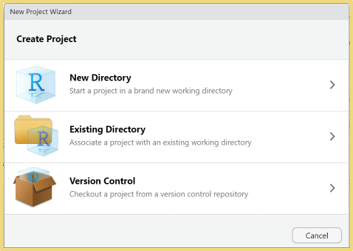
\includegraphics{Pictures/Ch0/CreateProject.png}
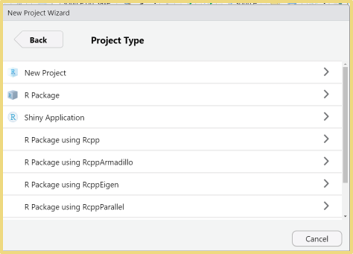
\includegraphics{Pictures/Ch0/Project.png}

\section{R Script Files}\label{r-script-files}

\begin{itemize}
\tightlist
\item
  Using R Script Files:

  \begin{itemize}
  \tightlist
  \item
    A .R script is simply a text file containing a set of commands and
    comments. The script can be saved and used later to rerun the code.
    The script can also be documented with comments and edited again and
    again to suit your needs.
  \end{itemize}
\item
  Using the Console

  \begin{itemize}
  \tightlist
  \item
    Entering and running code at the R command line is effective and
    simple. However, each time you want to execute a set of commands,
    you must re-enter them at the command line. Nothing saves for later.
  \end{itemize}
\item
  Complex commands are particularly difficult causing you to re-entering
  the code to fix any errors typographical or otherwise.R script files
  help to solve this issue.
\end{itemize}

\section{Create a New R Script File:
Chapter1.R}\label{create-a-new-r-script-file-chapter1.r}

\begin{itemize}
\tightlist
\item
  To save your notes from today's lecture, create a .R file named
  Chapter1.R and save it to your project file you made in the last
  class.
\item
  There are a couple of parts to this chapter, and we can add code from
  today's chapter in one file so that our code is stacked nicely
  together.\\
\item
  For each new chapter, start a new file and save it to your project
  folder.
\end{itemize}

\begin{figure}[H]

{\centering 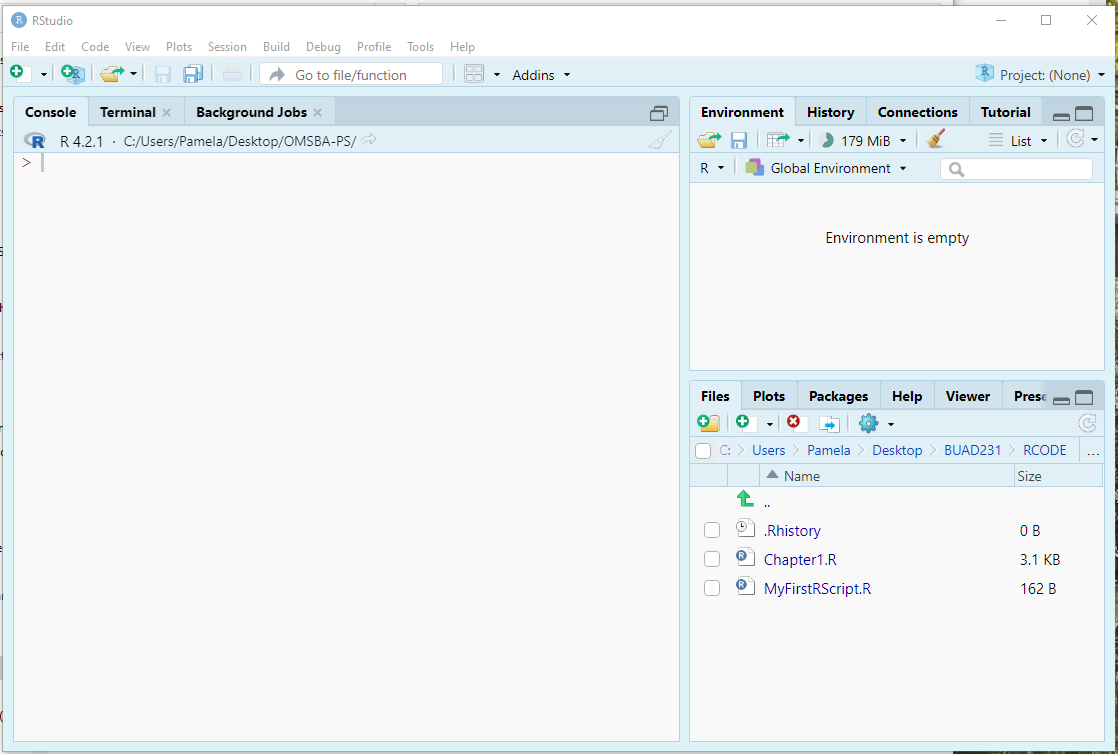
\includegraphics{Pictures/Ch1/RScript.png}

}

\caption{Screenshot of R Environment}

\end{figure}%

\section{Using a Prolog}\label{using-a-prolog}

\begin{itemize}
\tightlist
\item
  We should include a prolog to introduce each R Script File during the
  course.
\item
  A prolog is a set of comments at the top of a code file that provides
  information about what is in the file.
\item
  Including a prolog is considered coding best practice.
\item
  It also names the files and resources used that facilitates
  identification.
\item
  An informal prolog is below:
\end{itemize}

\begin{Shaded}
\begin{Highlighting}[]
\DocumentationTok{\#\#\#\#\#\#\#\#\#\#\#\#\#\#\#\#\#\#\#\#\#\#\#\#\#\#\#\#\#\#\#\#\#\#\#\#}
\CommentTok{\# Project name: }
\CommentTok{\# Project purpose: }
\CommentTok{\# Code author name: }
\CommentTok{\# Date last edited: }
\CommentTok{\# Data used: }
\CommentTok{\# Libraries used: }
\DocumentationTok{\#\#\#\#\#\#\#\#\#\#\#\#\#\#\#\#\#\#\#\#\#\#\#\#\#\#\#\#\#\#\#\#\#\#\#\#}
\end{Highlighting}
\end{Shaded}

\begin{itemize}
\tightlist
\item
  On your R Script File, add your own prolog following the template as
  shown.
\item
  I like to add a line for \emph{Data used} and \emph{Libraries used} so
  we know what all we used in the script.
\end{itemize}

\begin{Shaded}
\begin{Highlighting}[]
\DocumentationTok{\#\#\#\#\#\#\#\#\#\#\#\#\#\#\#\#\#\#\#\#\#\#\#\#\#\#\#\#\#\#\#\#\#\#\#\#}
\CommentTok{\# Project name: Chapter 1}
\CommentTok{\# Project purpose: To create an R script file to learn about R. }
\CommentTok{\# Code author name: Pamela Schlosser}
\CommentTok{\# Date last edited: [Enter Date Here]}
\CommentTok{\# Data used: NA}
\CommentTok{\# Libraries used: NA}
\DocumentationTok{\#\#\#\#\#\#\#\#\#\#\#\#\#\#\#\#\#\#\#\#\#\#\#\#\#\#\#\#\#\#\#\#\#\#\#\#}
\end{Highlighting}
\end{Shaded}

\begin{itemize}
\tightlist
\item
  Then, as we work through our .R script and add data files or libraries
  to our code, we go back and edit the prolog.
\end{itemize}

\section{R Handles Text in Multiple
Ways}\label{r-handles-text-in-multiple-ways}

\begin{itemize}
\tightlist
\item
  R can generally use single quotes or double quotes when marking text.
  However, if you use a single quote to start, use a single quote to
  end. The same for double quotes - ensure the pairing is the same quote
  type.
\item
  You sometimes need to be careful with nested quotes, but generally it
  does not matter which you use.
\end{itemize}

\begin{Shaded}
\begin{Highlighting}[]
\StringTok{"This is a string"}
\end{Highlighting}
\end{Shaded}

\begin{verbatim}
[1] "This is a string"
\end{verbatim}

\begin{Shaded}
\begin{Highlighting}[]
\StringTok{"This is also a string"}
\end{Highlighting}
\end{Shaded}

\begin{verbatim}
[1] "This is also a string"
\end{verbatim}

\begin{itemize}
\tightlist
\item
  We can also add comments to our code to document our work and add
  notes to our self or to others.
\end{itemize}

\begin{Shaded}
\begin{Highlighting}[]
\CommentTok{\# This is a comment for documentation or annotation}
\end{Highlighting}
\end{Shaded}

\begin{itemize}
\tightlist
\item
  Add the code above to your R file and run each line using Ctl + Enter
  or select all lines and click Run.
\item
  Take note that nothing prints in the console after running a comment.
\end{itemize}

\begin{figure}[H]

{\centering 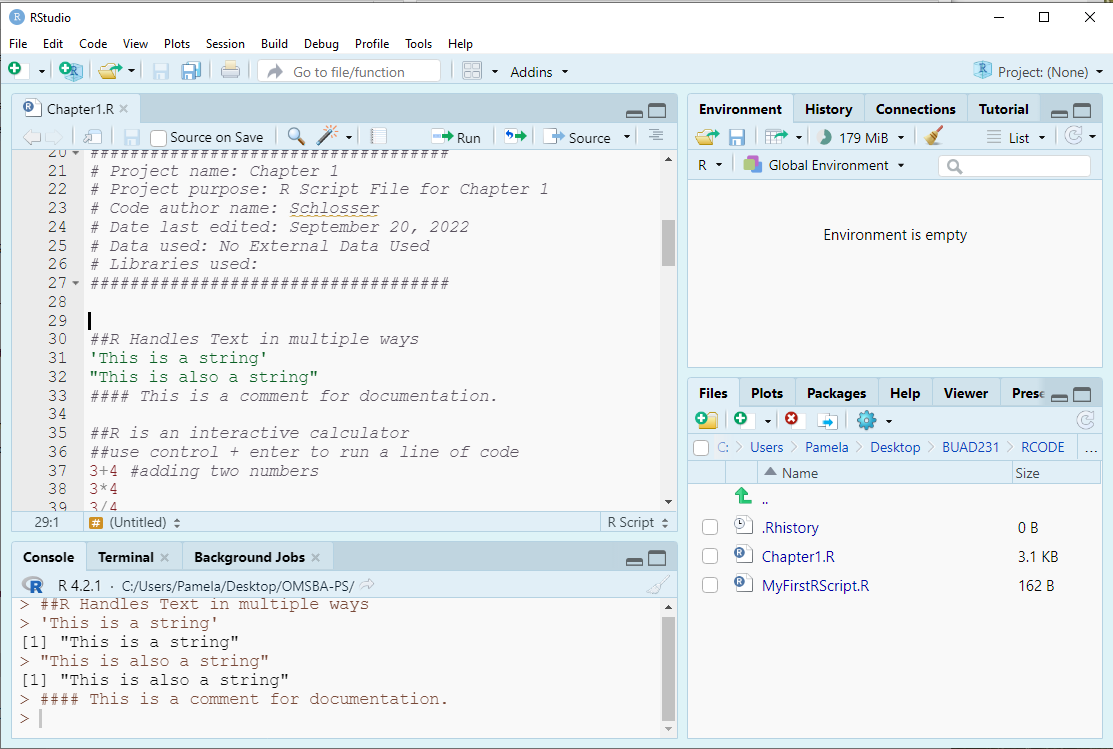
\includegraphics{Pictures/Ch1/Chapter1Start.png}

}

\caption{Chapter 1 R File}

\end{figure}%

\section{Using Comments}\label{using-comments}

\begin{itemize}
\tightlist
\item
  We use comments to organize and explain code in our R Script file.
\item
  Be sure to write clear code that does not need a lot of comments.
\item
  Include useful comments where needed so that anyone (including
  yourself in the future) can run and understand your code.
\item
  If something does not work, don't delete it yet. Instead, comment it
  out while you troubleshoot it or to try different alternatives.
\item
  Notice the prolog above is in comments.
\end{itemize}

\section{Note on R Markdown}\label{note-on-r-markdown}

\begin{itemize}
\tightlist
\item
  These files were formatted with RMarkdown. RMarkdown is a simple
  formatting syntax for authoring documents of a variety of types,
  including PowerPoint and html files.
\item
  On the document, RMarkdown prints the command and then follows the
  command with the output after 2 hashtags.
\item
  In your R Script File, you only need to type in the command and then
  run your code to get the same output as presented here.
\end{itemize}

\begin{figure}[H]

{\centering 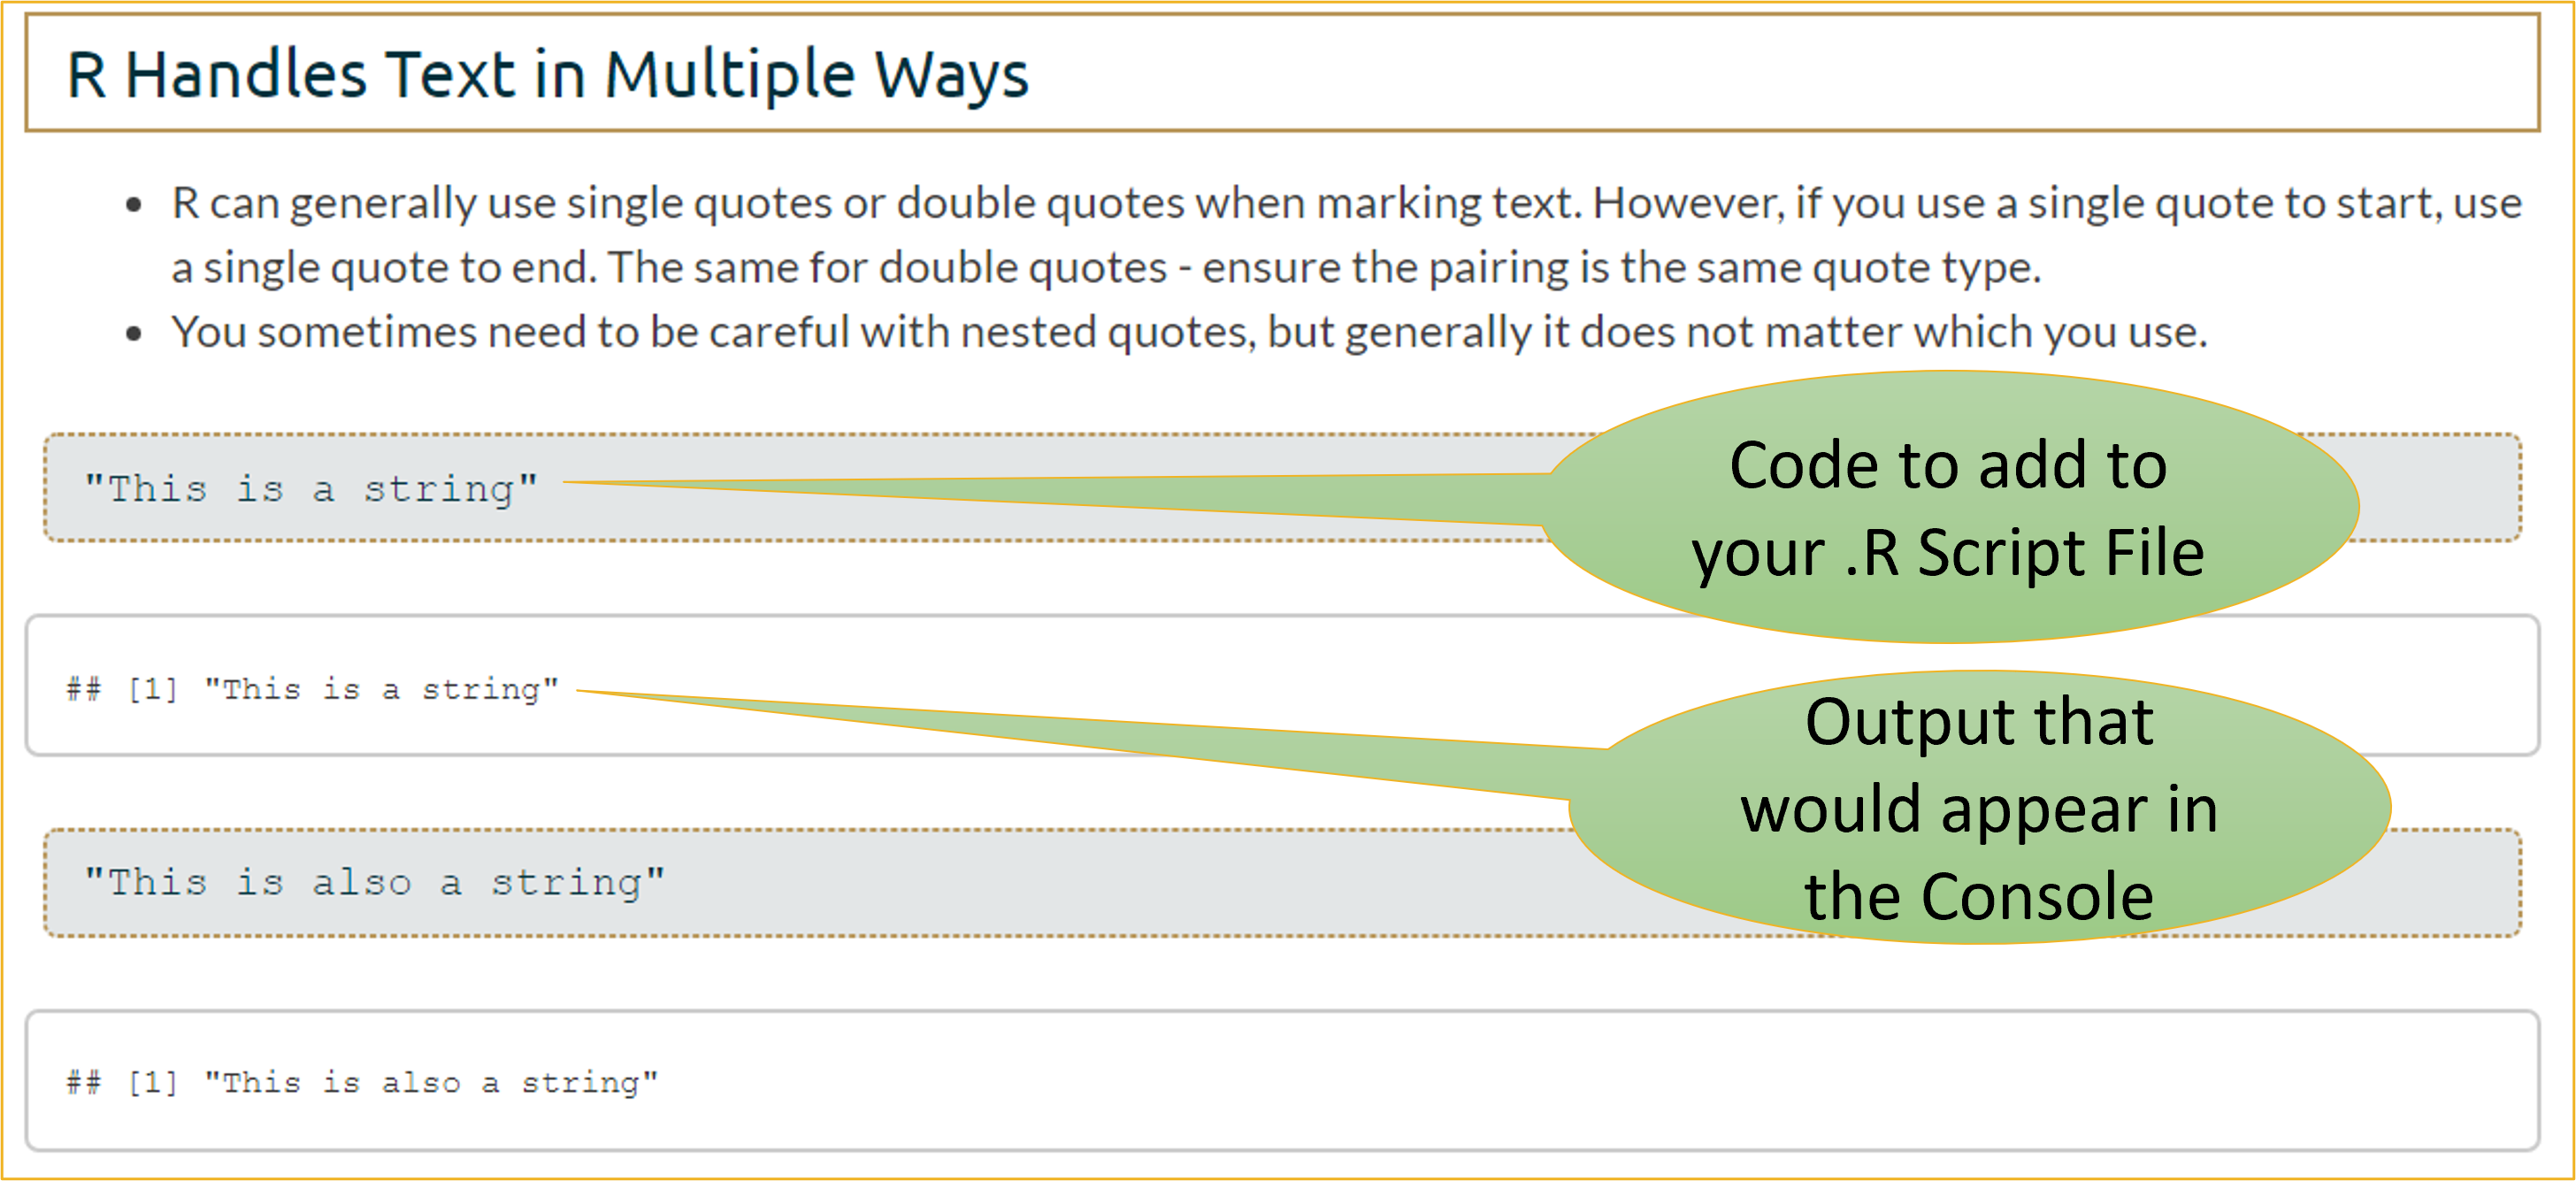
\includegraphics{Pictures/Ch1/ReadHTML.png}

}

\caption{Reading our HTML file}

\end{figure}%

\section{R is an Interactive
Calculator}\label{r-is-an-interactive-calculator}

\begin{itemize}
\tightlist
\item
  An important facet of R is that it should serve as your sole
  calculator.
\item
  Try these commands in your .R file by typing them in and clicking Ctr
  + Enter on each line.
\end{itemize}

\begin{Shaded}
\begin{Highlighting}[]
\DecValTok{3} \SpecialCharTok{+} \DecValTok{4}
\end{Highlighting}
\end{Shaded}

\begin{verbatim}
[1] 7
\end{verbatim}

\begin{Shaded}
\begin{Highlighting}[]
\DecValTok{3} \SpecialCharTok{*} \DecValTok{4}
\end{Highlighting}
\end{Shaded}

\begin{verbatim}
[1] 12
\end{verbatim}

\begin{Shaded}
\begin{Highlighting}[]
\DecValTok{3}\SpecialCharTok{/}\DecValTok{4}
\end{Highlighting}
\end{Shaded}

\begin{verbatim}
[1] 0.75
\end{verbatim}

\begin{Shaded}
\begin{Highlighting}[]
\DecValTok{3} \SpecialCharTok{+} \DecValTok{4} \SpecialCharTok{*} \DecValTok{100}\SpecialCharTok{\^{}}\DecValTok{2}
\end{Highlighting}
\end{Shaded}

\begin{verbatim}
[1] 40003
\end{verbatim}

\begin{itemize}
\tightlist
\item
  Take note that order of operations holds in R: PEMDAS

  \begin{itemize}
  \tightlist
  \item
    Parentheses ()
  \item
    Exponents \^{} and \(**\)
  \item
    Division \(/\), Multiplication \(*\), modulo, and integer division
  \item
    Addition + and Subtraction -
  \end{itemize}
\item
  Note that modulo and integer division have the same priority level as
  multiplication and division, where modulo is just the remainder.
\end{itemize}

\begin{Shaded}
\begin{Highlighting}[]
\FunctionTok{print}\NormalTok{(}\DecValTok{2} \SpecialCharTok{+} \DecValTok{3} \SpecialCharTok{*} \DecValTok{5} \SpecialCharTok{{-}} \DecValTok{7}\SpecialCharTok{\^{}}\DecValTok{2}\SpecialCharTok{\%\%}\DecValTok{4} \SpecialCharTok{+}\NormalTok{ (}\DecValTok{5}\SpecialCharTok{/}\DecValTok{2}\NormalTok{))}
\end{Highlighting}
\end{Shaded}

\begin{verbatim}
[1] 18.5
\end{verbatim}

\begin{Shaded}
\begin{Highlighting}[]
\DecValTok{5}\SpecialCharTok{/}\DecValTok{2}  \CommentTok{\#parentheses: = 2.5}
\end{Highlighting}
\end{Shaded}

\begin{verbatim}
[1] 2.5
\end{verbatim}

\begin{Shaded}
\begin{Highlighting}[]
\DecValTok{7}\SpecialCharTok{\^{}}\DecValTok{2}  \CommentTok{\#exponent:= 49}
\end{Highlighting}
\end{Shaded}

\begin{verbatim}
[1] 49
\end{verbatim}

\begin{Shaded}
\begin{Highlighting}[]
\DecValTok{3} \SpecialCharTok{*} \DecValTok{5}  \CommentTok{\#multiplication: = 15}
\end{Highlighting}
\end{Shaded}

\begin{verbatim}
[1] 15
\end{verbatim}

\begin{Shaded}
\begin{Highlighting}[]
\DecValTok{17}\SpecialCharTok{\%\%}\DecValTok{4}  \CommentTok{\#modulo: = 1}
\end{Highlighting}
\end{Shaded}

\begin{verbatim}
[1] 1
\end{verbatim}

\begin{Shaded}
\begin{Highlighting}[]
\DecValTok{17}\SpecialCharTok{\%/\%}\DecValTok{4}  \CommentTok{\#integer division: = 4}
\end{Highlighting}
\end{Shaded}

\begin{verbatim}
[1] 4
\end{verbatim}

\begin{Shaded}
\begin{Highlighting}[]
\DecValTok{2} \SpecialCharTok{+} \DecValTok{15}  \CommentTok{\#addition: = 17}
\end{Highlighting}
\end{Shaded}

\begin{verbatim}
[1] 17
\end{verbatim}

\begin{Shaded}
\begin{Highlighting}[]
\DecValTok{17} \SpecialCharTok{{-}} \DecValTok{1}  \CommentTok{\#subtraction: = 16}
\end{Highlighting}
\end{Shaded}

\begin{verbatim}
[1] 16
\end{verbatim}

\begin{Shaded}
\begin{Highlighting}[]
\DecValTok{16} \SpecialCharTok{+} \FloatTok{2.5}  \CommentTok{\#addition: = 18.5}
\end{Highlighting}
\end{Shaded}

\begin{verbatim}
[1] 18.5
\end{verbatim}

\section{Running Commands}\label{running-commands}

\begin{itemize}
\tightlist
\item
  There are a few ways to run commands via your .R file.

  \begin{itemize}
  \tightlist
  \item
    You can click Ctr + Enter on each line.
  \item
    You can select all the lines you want to run and select Ctr + Enter.
  \item
    You can select all the lines you want to run and select the run
    button as shown in the Figure.
  \end{itemize}
\end{itemize}

\begin{figure}[H]

{\centering 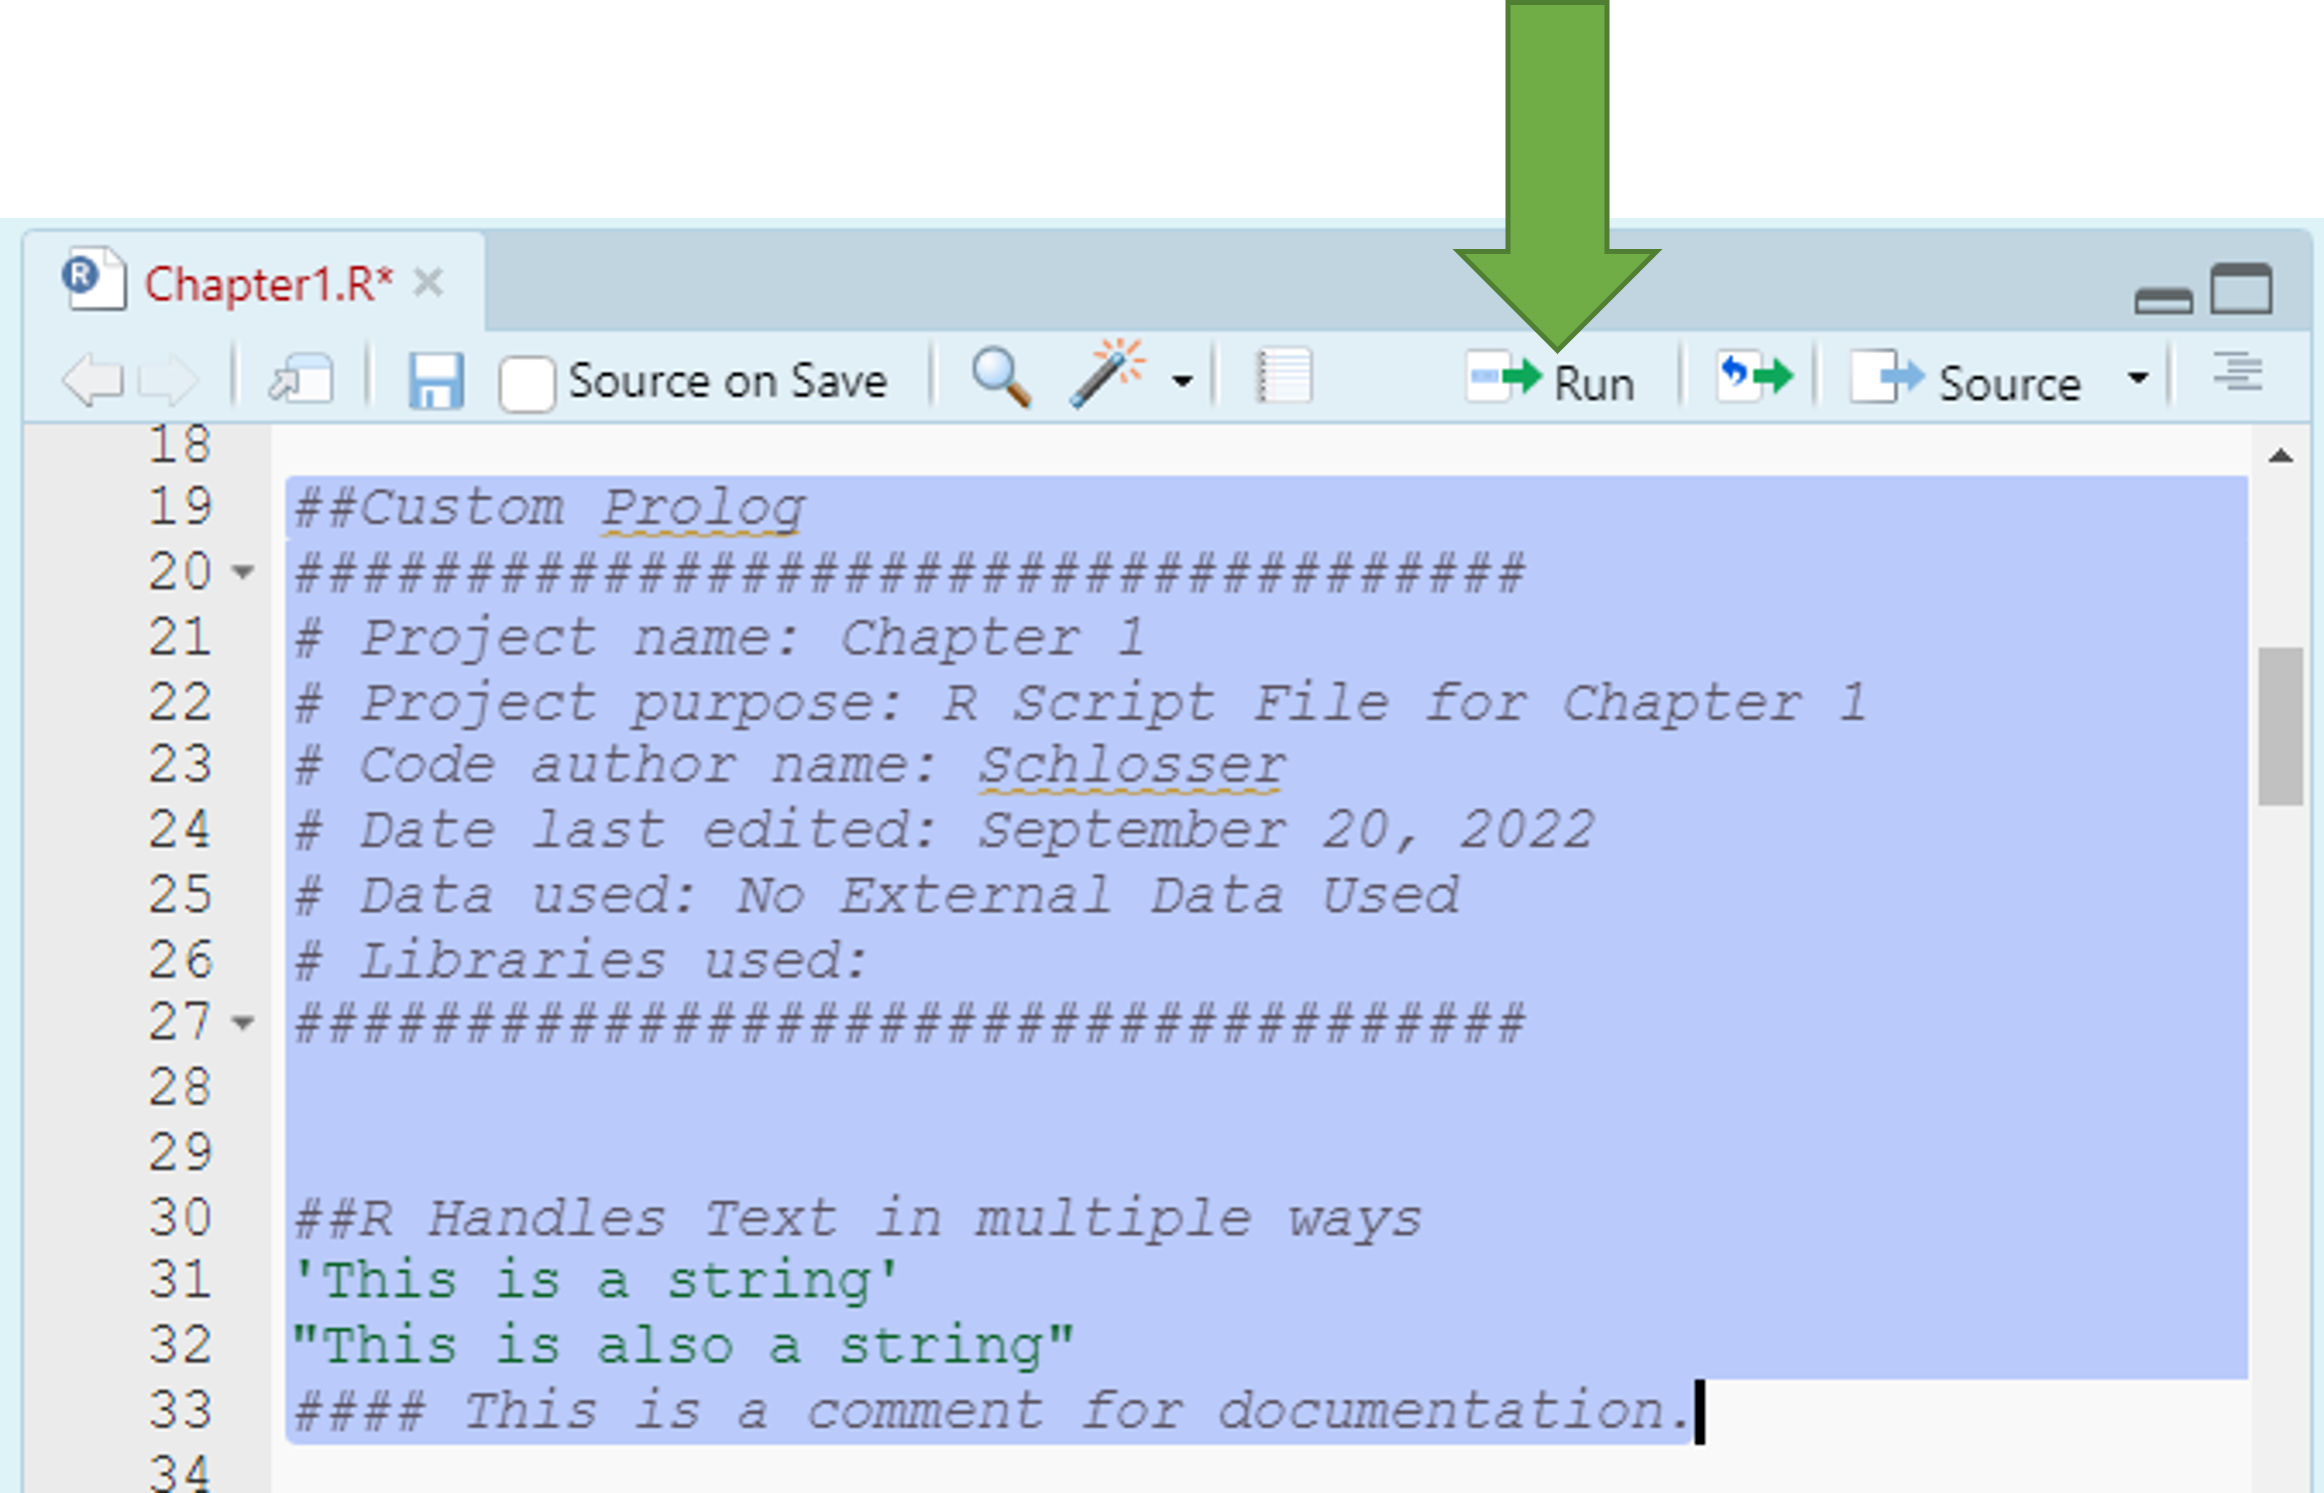
\includegraphics{Pictures/Ch1/Run.png}

}

\caption{Run Code}

\end{figure}%

\begin{itemize}
\tightlist
\item
  Now that I have asked you to add a couple lines of code, after this
  point, when R code is shown on this file, you should add it to your .R
  script file along with any notes you want. I won't explicitly say -
  ``add this code.''
\end{itemize}

\bookmarksetup{startatroot}

\chapter{Observations and Variables}\label{observations-and-variables}

\begin{itemize}
\item
  Going back to the basics in statistics, we need to define an
  observation and variable so that we can know how to use them
  effectively in R in creating objects.
\item
  An \emph{Observation} is a single row of data in a data frame that
  usually represents one person or other entity.
\item
  A \emph{Variable} is a measured characteristic of some entity (e.g.,
  income, years of education, sex, height, blood pressure, smoking
  status, etc.).
\item
  In data frames in R, the columns are variables that contain
  information about the observations (rows).

  \begin{itemize}
  \tightlist
  \item
    Note that we will break this code down later.
  \end{itemize}

\begin{Shaded}
\begin{Highlighting}[]
\NormalTok{income }\OtherTok{\textless{}{-}} \FunctionTok{c}\NormalTok{(}\DecValTok{34000}\NormalTok{, }\DecValTok{123000}\NormalTok{, }\DecValTok{215000}\NormalTok{)}
\NormalTok{voted }\OtherTok{\textless{}{-}} \FunctionTok{c}\NormalTok{(}\StringTok{"yes"}\NormalTok{, }\StringTok{"no"}\NormalTok{, }\StringTok{"no"}\NormalTok{)}
\NormalTok{vote }\OtherTok{\textless{}{-}} \FunctionTok{data.frame}\NormalTok{(income, voted)}
\NormalTok{vote}
\end{Highlighting}
\end{Shaded}

\begin{verbatim}
  income voted
1  34000   yes
2 123000    no
3 215000    no
\end{verbatim}
\item
  Observations: People being measured.
\item
  Variables: Information about each person (income and voted).
\end{itemize}

\begin{Shaded}
\begin{Highlighting}[]
\CommentTok{\# Shows the number of columns or variables}
\FunctionTok{ncol}\NormalTok{(vote)}
\end{Highlighting}
\end{Shaded}

\begin{verbatim}
[1] 2
\end{verbatim}

\begin{Shaded}
\begin{Highlighting}[]
\CommentTok{\# Shows the number of rows or observations}
\FunctionTok{nrow}\NormalTok{(vote)}
\end{Highlighting}
\end{Shaded}

\begin{verbatim}
[1] 3
\end{verbatim}

\begin{Shaded}
\begin{Highlighting}[]
\CommentTok{\# Shows both the number of rows (observations and columns}
\CommentTok{\# (variables).}
\FunctionTok{dim}\NormalTok{(vote)}
\end{Highlighting}
\end{Shaded}

\begin{verbatim}
[1] 3 2
\end{verbatim}

\section{The Assignment Operator in Creating
Objects}\label{the-assignment-operator-in-creating-objects}

\begin{itemize}
\tightlist
\item
  Entering and Storing Variables in R requires you to make an
  assignment.

  \begin{itemize}
  \tightlist
  \item
    We use the assignment operator `\textless-' to assign a value or
    expression to a variable.
  \item
    We typically do not use the = sign in R even though it works because
    it also means other things in R.
  \end{itemize}
\item
  Some examples are below to add to your .R file.
\end{itemize}

\begin{Shaded}
\begin{Highlighting}[]
\NormalTok{states }\OtherTok{\textless{}{-}} \DecValTok{29}
\NormalTok{A }\OtherTok{\textless{}{-}} \StringTok{"Apple"}
\CommentTok{\# Equivalent statement to above {-} again = is less used in R.}
\NormalTok{A }\OtherTok{=} \StringTok{"Apple"}
\FunctionTok{print}\NormalTok{(A)}
\end{Highlighting}
\end{Shaded}

\begin{verbatim}
[1] "Apple"
\end{verbatim}

\begin{Shaded}
\begin{Highlighting}[]
\CommentTok{\# Equivalent statement to above}
\NormalTok{A}
\end{Highlighting}
\end{Shaded}

\begin{verbatim}
[1] "Apple"
\end{verbatim}

\begin{Shaded}
\begin{Highlighting}[]
\NormalTok{B }\OtherTok{\textless{}{-}} \DecValTok{3} \SpecialCharTok{+} \DecValTok{4} \SpecialCharTok{*} \DecValTok{12}
\NormalTok{B}
\end{Highlighting}
\end{Shaded}

\begin{verbatim}
[1] 51
\end{verbatim}

\begin{figure}[H]

{\centering 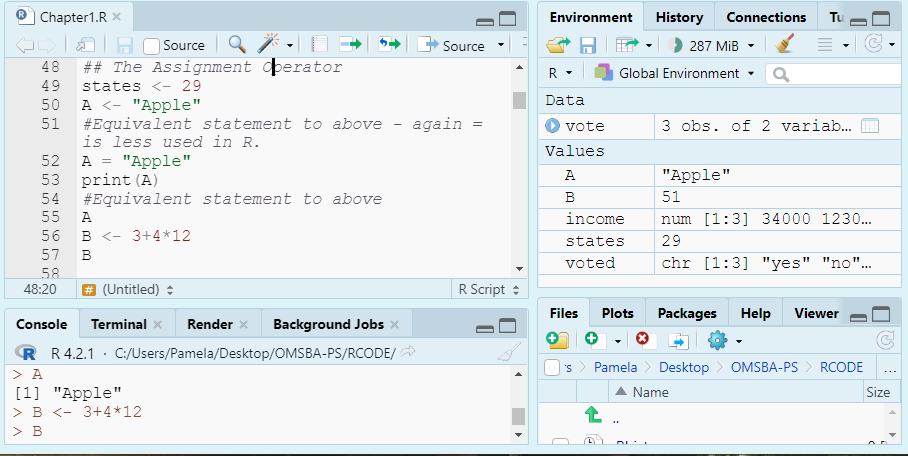
\includegraphics{Pictures/Ch1/Assignment.png}

}

\caption{The Assignment Operator}

\end{figure}%

\section{Naming Objects}\label{naming-objects}

\begin{itemize}
\tightlist
\item
  Line length limit: 80
\item
  Always use a consistent way of annotating code.
\item
  \emph{Camel case} is capitalizing the first letter of each word in the
  object name, with the exception of the first word.
\item
  \emph{Dot case} puts a dot between words in a variable name while
  camel case capitalizes each word in the variable name.
\item
  Object names appear on the left of assignment operator. We say an
  object receives or is assigned the value of the expression on the
  right.
\end{itemize}

\begin{enumerate}
\def\labelenumi{\arabic{enumi}.}
\tightlist
\item
  Naming Constants: A Constant contains a single numeric value.
\end{enumerate}

\begin{itemize}
\tightlist
\item
  The \emph{recommended} format for constants is starting with a ``k''
  and then using camel case. (e.g., kStates).
\end{itemize}

\begin{enumerate}
\def\labelenumi{\arabic{enumi}.}
\setcounter{enumi}{1}
\tightlist
\item
  Naming Functions: Functions are objects that perform a series of R
  commands to do something in particular.
\end{enumerate}

\begin{itemize}
\tightlist
\item
  The \emph{recommended} format for Functions is to use Camel case with
  the first letter capitalized. (e.g., MultiplyByTwo).
\end{itemize}

\begin{enumerate}
\def\labelenumi{\arabic{enumi}.}
\setcounter{enumi}{2}
\tightlist
\item
  Naming Variables: A Variable is a measured characteristic of some
  entity.
\end{enumerate}

\begin{itemize}
\item
  The \emph{recommended} format for variables is to use either the dot
  case or camel case. e.g., filled.script.month or filledScriptMonth.
\item
  A valid variable name consists of letters, numbers, along with the dot
  or underline characters.
\item
  A variable name must start with a letter, or the dot when not followed
  by a number.
\item
  A variable cannot contain spaces.
\item
  Variable names are case sensitive: x is different from X just as Age
  is different from AGE.
\item
  The value on the right must be a number, string, an expression, or
  another variable.
\item
  Some Examples Using Variable Rules:
\end{itemize}

\begin{Shaded}
\begin{Highlighting}[]
\NormalTok{AB}\FloatTok{.1} \OtherTok{\textless{}{-}} \StringTok{"Allowed?"}
\CommentTok{\# Does not follow rules {-} not allowed Try the statement below with no}
\CommentTok{\# hashtag to see the error message .123 \textless{}{-} \textquotesingle{}Allowed?\textquotesingle{}}
\NormalTok{A.A123 }\OtherTok{\textless{}{-}} \StringTok{"Allowed?"}
\NormalTok{G123AB }\OtherTok{\textless{}{-}} \StringTok{"Allowed?"}
\CommentTok{\# Recommended format for constants}
\NormalTok{kStates }\OtherTok{\textless{}{-}} \DecValTok{29}
\end{Highlighting}
\end{Shaded}

\begin{itemize}
\tightlist
\item
  Different R coders have different preferences, but consistency is key
  in making sure your code is easy to follow and for others to read. In
  this course, we will generally use the recommendation in the text
  which are listed above.
\item
  We tend to use one letter variable names (i.e., x) for placeholders or
  for simple functions (like naming a vector).
\end{itemize}

\bookmarksetup{startatroot}

\chapter{Built-in Functions}\label{built-in-functions}

\begin{itemize}
\tightlist
\item
  R has thousands of built-in functions including those for summary
  statistics. Below, we use a few built-in functions with constant
  numbers. The sqrt(), max(), and min() functions compute the square
  root of a number, and find the maximum and minimum numbers in a
  vector.
\end{itemize}

\begin{Shaded}
\begin{Highlighting}[]
\FunctionTok{sqrt}\NormalTok{(}\DecValTok{100}\NormalTok{)}
\end{Highlighting}
\end{Shaded}

\begin{verbatim}
[1] 10
\end{verbatim}

\begin{Shaded}
\begin{Highlighting}[]
\FunctionTok{max}\NormalTok{(}\DecValTok{100}\NormalTok{, }\DecValTok{200}\NormalTok{, }\DecValTok{300}\NormalTok{)}
\end{Highlighting}
\end{Shaded}

\begin{verbatim}
[1] 300
\end{verbatim}

\begin{Shaded}
\begin{Highlighting}[]
\FunctionTok{min}\NormalTok{(}\DecValTok{100}\NormalTok{, }\DecValTok{200}\NormalTok{, }\DecValTok{300}\NormalTok{)}
\end{Highlighting}
\end{Shaded}

\begin{verbatim}
[1] 100
\end{verbatim}

\begin{itemize}
\item
  We can also create variables to use within built-in functions.
\item
  Below, we create a vector x and use a few built-in functions as
  examples.

  \begin{itemize}
  \tightlist
  \item
    The sort() function sorts a vector from small to large.
  \end{itemize}

\begin{Shaded}
\begin{Highlighting}[]
\NormalTok{x }\OtherTok{\textless{}{-}} \FunctionTok{c}\NormalTok{(}\DecValTok{1}\NormalTok{, }\DecValTok{2}\NormalTok{, }\DecValTok{3}\NormalTok{, }\DecValTok{3}\NormalTok{, }\DecValTok{100}\NormalTok{, }\SpecialCharTok{{-}}\DecValTok{10}\NormalTok{, }\DecValTok{40}\NormalTok{)  }\CommentTok{\#Creating a Vector x}
\FunctionTok{sort}\NormalTok{(x)  }\CommentTok{\#Sorting the Vector x from Small to Large}
\end{Highlighting}
\end{Shaded}

\begin{verbatim}
[1] -10   1   2   3   3  40 100
\end{verbatim}

\begin{Shaded}
\begin{Highlighting}[]
\FunctionTok{max}\NormalTok{(x)  }\CommentTok{\#Finding Largest Element of Vector x}
\end{Highlighting}
\end{Shaded}

\begin{verbatim}
[1] 100
\end{verbatim}

\begin{Shaded}
\begin{Highlighting}[]
\FunctionTok{min}\NormalTok{(x)  }\CommentTok{\#Finding Smallest Element of Vector x}
\end{Highlighting}
\end{Shaded}

\begin{verbatim}
[1] -10
\end{verbatim}
\end{itemize}

\section{Built-in Functions: Setting an
Argument}\label{built-in-functions-setting-an-argument}

\begin{itemize}
\tightlist
\item
  The standard format to a built-in function is functionName(argument)

  \begin{itemize}
  \tightlist
  \item
    For example, the square root function structure is listed as
    sqrt(x), where x is a numeric or complex vector or array.
  \end{itemize}
\end{itemize}

\begin{Shaded}
\begin{Highlighting}[]
\CommentTok{\# Here, we are setting a required argument x to a value of 100. When}
\CommentTok{\# a value is set, it turns it to a parameter of the function.}
\FunctionTok{sqrt}\NormalTok{(}\AttributeTok{x =} \DecValTok{100}\NormalTok{)}
\end{Highlighting}
\end{Shaded}

\begin{verbatim}
[1] 10
\end{verbatim}

\begin{Shaded}
\begin{Highlighting}[]
\CommentTok{\# Because there is only one argument and it is required, we can}
\CommentTok{\# eliminate its name x= from our function call. This is discussed}
\CommentTok{\# below.}
\FunctionTok{sqrt}\NormalTok{(}\DecValTok{100}\NormalTok{)}
\end{Highlighting}
\end{Shaded}

\begin{verbatim}
[1] 10
\end{verbatim}

\begin{itemize}
\tightlist
\item
  There is a little variety in how we can write functions to get the
  same results.
\item
  A parameter is what a function can take as input. It is a placeholder
  and hence does not have a concrete value. An argument is a value
  passed during function invocation.
\item
  There are some default values set up in R in which arguments have
  already been set.
\item
  There are a few functions with no parameters like Sys.time() which
  produces the date and time. If you are not sure how many parameters a
  function has, you should look it up in the help.
\end{itemize}

\section{Default Values}\label{default-values}

\begin{itemize}
\tightlist
\item
  There are many default values set up in R in which arguments have
  already been set to a particular value or field.
\item
  Default values have been set when you see the = value in the
  instructions. If we don't want to change it, we don't need to include
  it in our function call.
\item
  When only one argument is required, the argument is usually not set to
  have a default value.
\end{itemize}

\section{Built-in Functions: Using More than One
Argument}\label{built-in-functions-using-more-than-one-argument}

\begin{itemize}
\tightlist
\item
  For functions with more than one parameter, we must determine what
  arguments we want to include, and whether a default value was set and
  if we want to change it. Default values have been set when you see the
  = value in the instructions. If we don't want to change it, we don't
  need to include it in our function call.

  \begin{itemize}
  \tightlist
  \item
    For example, the default S3 method for the seq() function is listed
    as the following: seq(from = 1, to = 1, by = ((to -
    from)/(length.out - 1)),length.out = NULL, along.with = NULL,
    \ldots)
  \item
    Default values have been set on each parameter, but we can change
    some of them to get a meaningful result.
  \item
    For example, we set the from, to, and by parameter to get a sequence
    from 0 to 30 in increments of 5.
  \end{itemize}
\end{itemize}

\begin{Shaded}
\begin{Highlighting}[]
\CommentTok{\# We can use the following code.}
\FunctionTok{seq}\NormalTok{(}\AttributeTok{from =} \DecValTok{0}\NormalTok{, }\AttributeTok{to =} \DecValTok{30}\NormalTok{, }\AttributeTok{by =} \DecValTok{5}\NormalTok{)}
\end{Highlighting}
\end{Shaded}

\begin{verbatim}
[1]  0  5 10 15 20 25 30
\end{verbatim}

\begin{itemize}
\item
  We can simplify this function call even further:

  \begin{itemize}
  \tightlist
  \item
    If we use the same order of parameters as the instructions, we can
    eliminate the \emph{argument=} from the function.
  \item
    Since we do list the values to the arguments in same order as the
    function is defined, we can eliminate the from=, to=, and by= to
    simplify the statement.
  \end{itemize}

\begin{Shaded}
\begin{Highlighting}[]
\CommentTok{\# Equivalent statement as above}
\FunctionTok{seq}\NormalTok{(}\DecValTok{0}\NormalTok{, }\DecValTok{30}\NormalTok{, }\DecValTok{5}\NormalTok{)}
\end{Highlighting}
\end{Shaded}

\begin{verbatim}
[1]  0  5 10 15 20 25 30
\end{verbatim}
\item
  If you leave off the by parameter, it defaults at 1.
\end{itemize}

\begin{Shaded}
\begin{Highlighting}[]
\CommentTok{\# Leaving by= to default value of 1}
\FunctionTok{seq}\NormalTok{(}\DecValTok{0}\NormalTok{, }\DecValTok{30}\NormalTok{)}
\end{Highlighting}
\end{Shaded}

\begin{verbatim}
 [1]  0  1  2  3  4  5  6  7  8  9 10 11 12 13 14 15 16 17 18 19 20 21 22 23 24
[26] 25 26 27 28 29 30
\end{verbatim}

\begin{itemize}
\tightlist
\item
  There can be a little hurdle deciding when you need the argument value
  in the function call. The general rule is that if you don't know,
  include it. If it makes more sense to you to include it, include it.
\end{itemize}

\section{Tips on Arguments}\label{tips-on-arguments}

\begin{itemize}
\tightlist
\item
  Always look up a built-in function to see the arguments you can use.
\item
  Arguments are always named when you define a function.
\item
  When you call a function, you do not have to specify the name of the
  argument.
\item
  Arguments have default values, which is used if you do not specify a
  value for that argument yourself.
\item
  An argument list comprises of comma-separated values that contain the
  various formal arguments.
\item
  Default arguments are specified as follows: \emph{parameter =
  expression}
\end{itemize}

\begin{Shaded}
\begin{Highlighting}[]
\NormalTok{y }\OtherTok{\textless{}{-}} \DecValTok{10}\SpecialCharTok{:}\DecValTok{20}
\FunctionTok{sort}\NormalTok{(y)}
\end{Highlighting}
\end{Shaded}

\begin{verbatim}
 [1] 10 11 12 13 14 15 16 17 18 19 20
\end{verbatim}

\begin{Shaded}
\begin{Highlighting}[]
\FunctionTok{sort}\NormalTok{(y, }\AttributeTok{decreasing =} \ConstantTok{FALSE}\NormalTok{)}
\end{Highlighting}
\end{Shaded}

\begin{verbatim}
 [1] 10 11 12 13 14 15 16 17 18 19 20
\end{verbatim}

\section{Saving}\label{saving}

\begin{itemize}
\tightlist
\item
  You can save your work in the file menu or the save shortcut using
  Ctrl + S or Cmd+S depending on your Operating System.
\item
  You will routinely be asked to save your workspace image, and you
  don't need to save this unless specifically asked. It saves the output
  we have generated so far.
\item
  You can stop this from happening by setting the Tools \textgreater{}
  Global Options \textgreater{} Under Workspace changing this to Never.
\item
  Be careful with this option because it won't save what you don't run.
\end{itemize}

\begin{figure}[H]

{\centering 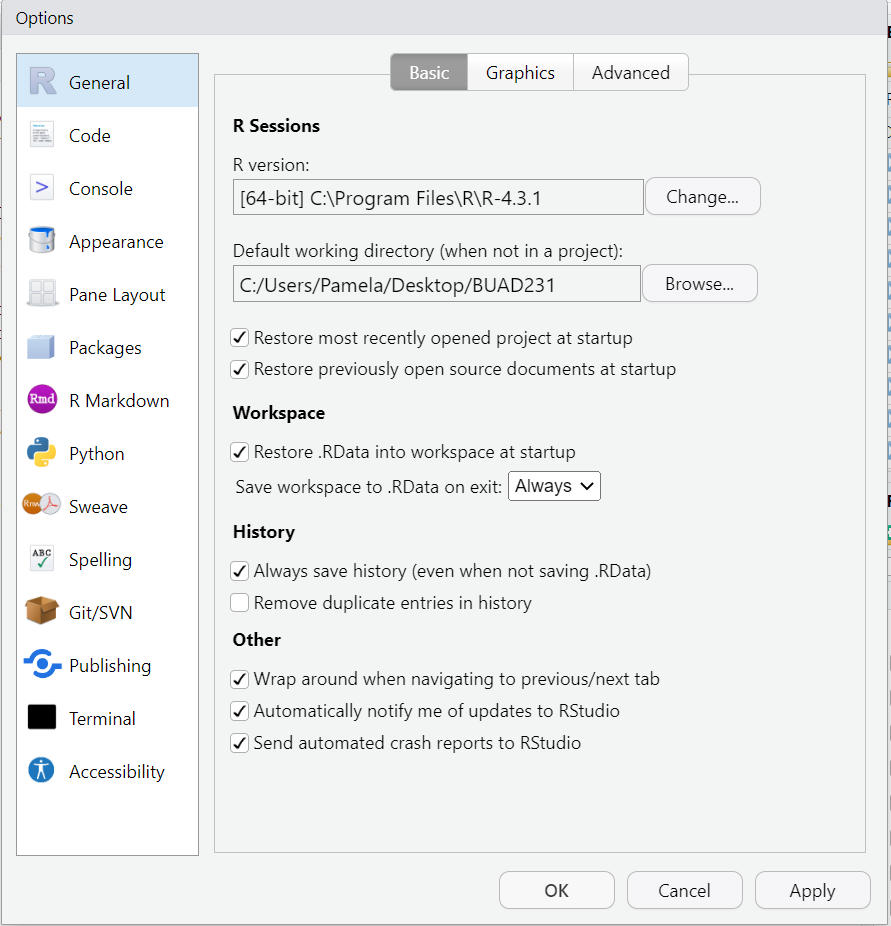
\includegraphics{Pictures/Ch1/SaveOptions.png}

}

\caption{Evalulating Your Environment}

\end{figure}%

\section{Calling a Library}\label{calling-a-library}

\begin{itemize}
\tightlist
\item
  In R, a package is a collection of R functions, data and compiled
  code. The location where the packages are stored is called the
  library.
\item
  Libraries need to be activated one time in each new R session.
\item
  You can access a function from a library one time using
  library::function()
\end{itemize}

\begin{Shaded}
\begin{Highlighting}[]
\CommentTok{\# Use to activate library in an R session.}
\FunctionTok{library}\NormalTok{(tidyverse)}
\FunctionTok{library}\NormalTok{(dplyr)}
\end{Highlighting}
\end{Shaded}

\begin{itemize}
\tightlist
\item
  You can access a function from a library one time only using
  library::function()

  \begin{itemize}
  \tightlist
  \item
    Useful if only using one function from the library.
  \end{itemize}
\item
  We will return to this in data prep.
\end{itemize}

\begin{Shaded}
\begin{Highlighting}[]
\DocumentationTok{\#\# Below is an example that would use dplyr for one select function}
\DocumentationTok{\#\# to select variable1 from the oldData and save it as a new object}
\DocumentationTok{\#\# NewData. Since we don’t have datasets yet, we will revisit this.}
\DocumentationTok{\#\# NewData \textless{}{-} dplyr::select(oldData, variable1)}
\end{Highlighting}
\end{Shaded}

\begin{itemize}
\tightlist
\item
  Some libraries are part of other global libraries:

  \begin{itemize}
  \tightlist
  \item
    dplyr is part of tidyverse, there is actually no need to activate it
    if tidyverse is active, however, sometimes it helps when conflicts
    are present
  \item
    An example of a conflict is the use of a select function which shows
    up in both the dplyr and MASS package. If both libraries are active,
    R does not know which to use.
  \item
    tidyverse has many libraries included in it.
  \end{itemize}
\end{itemize}

\section{The Environment}\label{the-environment}

\begin{itemize}
\tightlist
\item
  You can evaluate your Environment Tab to see your Variables we have
  defined in R Studio.
\item
  Use the following functions to view and remove defined variables in
  your Global Environment
\end{itemize}

\begin{Shaded}
\begin{Highlighting}[]
\FunctionTok{ls}\NormalTok{()  }\CommentTok{\#Lists all variables in Global Environment }
\end{Highlighting}
\end{Shaded}

\begin{verbatim}
 [1] "A"       "A.A123"  "AB.1"    "B"       "G123AB"  "income"  "kStates"
 [8] "states"  "vote"    "voted"   "x"       "y"      
\end{verbatim}

\begin{Shaded}
\begin{Highlighting}[]
\FunctionTok{rm}\NormalTok{(states)  }\CommentTok{\#Removes variable named states}
\FunctionTok{rm}\NormalTok{(}\AttributeTok{list =} \FunctionTok{ls}\NormalTok{())  }\CommentTok{\#Clears all variables from Global Environment}
\end{Highlighting}
\end{Shaded}

\begin{figure}[H]

{\centering 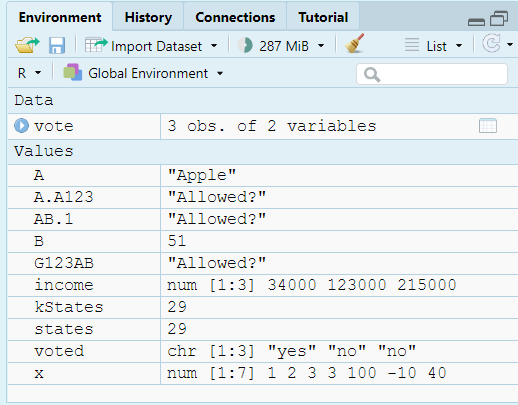
\includegraphics{Pictures/Ch1/Environment.png}

}

\caption{Evalulating Your RStudio Environment}

\end{figure}%

\bookmarksetup{startatroot}

\chapter{Entering and Loading Data}\label{entering-and-loading-data}

\section{Creating a Vector}\label{creating-a-vector}

\begin{itemize}
\tightlist
\item
  A vector is the simplest type of data structure in R.

  \begin{itemize}
  \tightlist
  \item
    A vector is a set of data elements that are saved together as the
    same type.
  \item
    We have many ways to create vectors with some examples below.
  \end{itemize}
\item
  Use c() function, which is a generic function which combines its
  arguments into a vector or list.
\end{itemize}

\begin{Shaded}
\begin{Highlighting}[]
\FunctionTok{c}\NormalTok{(}\DecValTok{1}\NormalTok{, }\DecValTok{2}\NormalTok{, }\DecValTok{3}\NormalTok{, }\DecValTok{4}\NormalTok{, }\DecValTok{5}\NormalTok{)  }\CommentTok{\#Print a Vector 1:5}
\end{Highlighting}
\end{Shaded}

\begin{verbatim}
[1] 1 2 3 4 5
\end{verbatim}

\begin{itemize}
\tightlist
\item
  If numbers are aligned, can use the ``:`` symbol to include numbers
  and all in between. This is considered an array.
\end{itemize}

\begin{Shaded}
\begin{Highlighting}[]
\DecValTok{1}\SpecialCharTok{:}\DecValTok{5}  \CommentTok{\#Print a Vector 1:5}
\end{Highlighting}
\end{Shaded}

\begin{verbatim}
[1] 1 2 3 4 5
\end{verbatim}

\begin{itemize}
\tightlist
\item
  Use seq() function to make a vector given a sequence.
\end{itemize}

\begin{Shaded}
\begin{Highlighting}[]
\FunctionTok{seq}\NormalTok{(}\AttributeTok{from =} \DecValTok{0}\NormalTok{, }\AttributeTok{to =} \DecValTok{30}\NormalTok{, }\AttributeTok{by =} \DecValTok{5}\NormalTok{)  }\CommentTok{\#Creates a sequence vector from 0 to 30 in increments on 5 }
\end{Highlighting}
\end{Shaded}

\begin{verbatim}
[1]  0  5 10 15 20 25 30
\end{verbatim}

\begin{itemize}
\tightlist
\item
  Use rep() function to repeat the elements of a vector.
\end{itemize}

\begin{Shaded}
\begin{Highlighting}[]
\FunctionTok{rep}\NormalTok{(}\AttributeTok{x =} \DecValTok{1}\SpecialCharTok{:}\DecValTok{3}\NormalTok{, }\AttributeTok{times =} \DecValTok{4}\NormalTok{)  }\CommentTok{\#Repeat the elements of the vector 4 times}
\end{Highlighting}
\end{Shaded}

\begin{verbatim}
 [1] 1 2 3 1 2 3 1 2 3 1 2 3
\end{verbatim}

\begin{Shaded}
\begin{Highlighting}[]
\FunctionTok{rep}\NormalTok{(}\AttributeTok{x =} \DecValTok{1}\SpecialCharTok{:}\DecValTok{3}\NormalTok{, }\AttributeTok{each =} \DecValTok{3}\NormalTok{)  }\CommentTok{\#Repeat the elements of a vector 3 times each}
\end{Highlighting}
\end{Shaded}

\begin{verbatim}
[1] 1 1 1 2 2 2 3 3 3
\end{verbatim}

\section{Creating a Matrix}\label{creating-a-matrix}

\begin{itemize}
\item
  A matrix is another type of object like a vector or a list.

  \begin{itemize}
  \tightlist
  \item
    A matrix has a rectangular format with rows and columns.
  \item
    A matrix uses matrix() function
  \item
    You can include the byrow = argument to tell the function whether to
    fill across or down first.
  \item
    You can also include the dimnames() function in addition to the
    matrix() to assign names to rows and columns.
  \end{itemize}
\item
  Using matrix() function, we can create a matrix with 3 rows and 3
  columns as shown below.

  \begin{itemize}
  \tightlist
  \item
    Take note how the matrix fills in the new data.
  \end{itemize}

\begin{Shaded}
\begin{Highlighting}[]
\CommentTok{\# Creating a Variable X that has 9 Values.}
\NormalTok{x }\OtherTok{\textless{}{-}} \DecValTok{1}\SpecialCharTok{:}\DecValTok{9}
\CommentTok{\# Setting the matrix.}
\FunctionTok{matrix}\NormalTok{(x, }\AttributeTok{nrow =} \DecValTok{3}\NormalTok{, }\AttributeTok{ncol =} \DecValTok{3}\NormalTok{)}
\end{Highlighting}
\end{Shaded}

\begin{verbatim}
     [,1] [,2] [,3]
[1,]    1    4    7
[2,]    2    5    8
[3,]    3    6    9
\end{verbatim}

\begin{Shaded}
\begin{Highlighting}[]
\CommentTok{\# Note – we do not need to name the arguments because we go in the}
\CommentTok{\# correct order.  The function below simplifies the statement and}
\CommentTok{\# provides the same answer as above.}
\FunctionTok{matrix}\NormalTok{(x, }\DecValTok{3}\NormalTok{, }\DecValTok{3}\NormalTok{)}
\end{Highlighting}
\end{Shaded}

\begin{verbatim}
     [,1] [,2] [,3]
[1,]    1    4    7
[2,]    2    5    8
[3,]    3    6    9
\end{verbatim}
\end{itemize}

\subsection{Setting More Arguments in a
Matrix}\label{setting-more-arguments-in-a-matrix}

\begin{itemize}
\tightlist
\item
  The byrow argument fills the Matrix across the row
\item
  Below, we can use the byrow statement and assign it to a variable m.
\end{itemize}

\begin{Shaded}
\begin{Highlighting}[]
\NormalTok{m }\OtherTok{\textless{}{-}} \FunctionTok{matrix}\NormalTok{(}\DecValTok{1}\SpecialCharTok{:}\DecValTok{9}\NormalTok{, }\DecValTok{3}\NormalTok{, }\DecValTok{3}\NormalTok{, }\AttributeTok{byrow =} \ConstantTok{TRUE}\NormalTok{)  }\CommentTok{\#Fills the Matrix Across the Row and assigns it to variable m}
\NormalTok{m  }\CommentTok{\#Printing the matrix in the console}
\end{Highlighting}
\end{Shaded}

\begin{verbatim}
     [,1] [,2] [,3]
[1,]    1    2    3
[2,]    4    5    6
[3,]    7    8    9
\end{verbatim}

\begin{itemize}
\tightlist
\item
  The dimnames() function adds labels to either the row and the column.
  In this case below both are added to our matrix m.
\end{itemize}

\begin{Shaded}
\begin{Highlighting}[]
\FunctionTok{dimnames}\NormalTok{(}\AttributeTok{x =}\NormalTok{ m) }\OtherTok{\textless{}{-}} \FunctionTok{list}\NormalTok{(}\FunctionTok{c}\NormalTok{(}\StringTok{"2020"}\NormalTok{, }\StringTok{"2021"}\NormalTok{, }\StringTok{"2022"}\NormalTok{), }\FunctionTok{c}\NormalTok{(}\StringTok{"low"}\NormalTok{, }\StringTok{"medium"}\NormalTok{, }\StringTok{"high"}\NormalTok{))}
\NormalTok{m  }\CommentTok{\#Printing the matrix in the console}
\end{Highlighting}
\end{Shaded}

\begin{verbatim}
     low medium high
2020   1      2    3
2021   4      5    6
2022   7      8    9
\end{verbatim}

\begin{itemize}
\tightlist
\item
  You try to make a matrix of 25 items, or a 5 by 5, and fill the matrix
  across the row and assign the matrix to the name m2.
\item
  You should get the answer below.
\end{itemize}

\begin{verbatim}
     [,1] [,2] [,3] [,4] [,5]
[1,]    1    2    3    4    5
[2,]    6    7    8    9   10
[3,]   11   12   13   14   15
[4,]   16   17   18   19   20
[5,]   21   22   23   24   25
\end{verbatim}

\subsection{Differences between Data Frames and
Matrices}\label{differences-between-data-frames-and-matrices}

\begin{itemize}
\tightlist
\item
  In a data frame the columns contain different types of data, but in a
  matrix all the elements are the same type of data. A matrix is usually
  numbers.
\item
  A matrix can be looked at as a vector with additional methods or
  dimensions, while a data frame is a list.
\end{itemize}

\section{Creating a Data Frame}\label{creating-a-data-frame}

\begin{itemize}
\tightlist
\item
  A data frame is a table or a two-dimensional array-like structure in
  which each column contains values of one variable and each row
  contains one set of values from each column. In a data frame the rows
  are observations and columns are variables.

  \begin{itemize}
  \tightlist
  \item
    Data frames are generic data objects to store tabular data.
  \item
    The column names should be non-empty.
  \item
    The row names should be unique.
  \item
    The data stored in a data frame can be of numeric, factor or
    character type.
  \item
    Each column should contain same number of data items.
  \item
    Combing vectors into a data frame using the data.frame() function
  \end{itemize}
\item
  Below, we can create vectors for state, year enacted, personal oz
  limit medical marijuana.
\end{itemize}

\begin{Shaded}
\begin{Highlighting}[]
\NormalTok{state }\OtherTok{\textless{}{-}} \FunctionTok{c}\NormalTok{(}\StringTok{"Alaska"}\NormalTok{, }\StringTok{"Arizona"}\NormalTok{, }\StringTok{"Arkansas"}\NormalTok{)}
\NormalTok{year.legal }\OtherTok{\textless{}{-}} \FunctionTok{c}\NormalTok{(}\DecValTok{1998}\NormalTok{, }\DecValTok{2010}\NormalTok{, }\DecValTok{2016}\NormalTok{)}
\NormalTok{ounce.lim }\OtherTok{\textless{}{-}} \FunctionTok{c}\NormalTok{(}\DecValTok{1}\NormalTok{, }\FloatTok{2.5}\NormalTok{, }\DecValTok{3}\NormalTok{)}
\end{Highlighting}
\end{Shaded}

\begin{itemize}
\tightlist
\item
  Then, we can combine the 3 vectors into a data frame and name the data
  frame pot.legal.
\end{itemize}

\begin{Shaded}
\begin{Highlighting}[]
\NormalTok{pot.legal }\OtherTok{\textless{}{-}} \FunctionTok{data.frame}\NormalTok{(state, year.legal, ounce.lim)}
\end{Highlighting}
\end{Shaded}

\begin{itemize}
\tightlist
\item
  Next, check your global environment to confirm data frame was created.
\end{itemize}

\begin{figure}[H]

{\centering 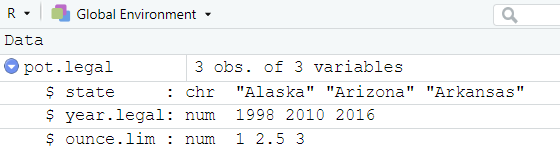
\includegraphics{Pictures/Ch1/DataFrame.png}

}

\caption{Global Environment}

\end{figure}%

\section{Importing a Data Frame into
R}\label{importing-a-data-frame-into-r}

\begin{itemize}
\tightlist
\item
  When importing data from outside sources, you can do the following:
\end{itemize}

\begin{enumerate}
\def\labelenumi{\arabic{enumi}.}
\tightlist
\item
  You can import data from an R package using data() function.
\item
  You can also link directly to a file on the web.
\item
  You can import data through from your computer through common file
  extensions:

  \begin{itemize}
  \tightlist
  \item
    .csv: comma separated values;
  \item
    .txt: text file;
  \item
    .xls or .xlsx: Excel file;
  \item
    .sav: SPSS file;
  \item
    .sasb7dat: SAS file;
  \item
    .xpt: SAS transfer file;
  \item
    .dta: Stata file.
  \end{itemize}
\end{enumerate}

\begin{itemize}
\tightlist
\item
  Each different file type requires a unique function to read in the
  file. With all the variety in file types, it is best to look it up in
  the R Community to help.
\end{itemize}

\subsection{Use data() function}\label{use-data-function}

\begin{itemize}
\tightlist
\item
  All we need is the data() function to read in a data set that is part
  of R. R has many built in libraries now, so there are many data sets
  we can use for testing and learning statistics in R.
\end{itemize}

\begin{Shaded}
\begin{Highlighting}[]
\CommentTok{\# The mtcars data set is part of R, so no new package needs to be}
\CommentTok{\# downloaded.}
\FunctionTok{data}\NormalTok{(}\StringTok{"mtcars"}\NormalTok{)}
\end{Highlighting}
\end{Shaded}

\begin{itemize}
\item
  Load a data frame from a unique package in R.

  \begin{itemize}
  \tightlist
  \item
    There are also a lot of packages that house data sets. It is fairly
    easy to make a package that contains data and load it into CRAN.
    These packages need to be installed into your R one time. Then, each
    time you open R, you need to reload the library using the library()
    function.
  \item
    When your run the install.packages() function, do not include the \#
    symbol. Then, after you run it one time, comment it out. There is no
    need to run this code a second time unless something happens to your
    RStudio.
  \end{itemize}

\begin{Shaded}
\begin{Highlighting}[]
\CommentTok{\# install.packages(\textquotesingle{}MASS\textquotesingle{}) \#only need to install package one time in}
\CommentTok{\# R}
\FunctionTok{library}\NormalTok{(MASS)}
\end{Highlighting}
\end{Shaded}
\end{itemize}

\begin{Shaded}
\begin{Highlighting}[]
\FunctionTok{data}\NormalTok{(}\StringTok{"Insurance"}\NormalTok{)}
\FunctionTok{head}\NormalTok{(Insurance)}
\end{Highlighting}
\end{Shaded}

\begin{verbatim}
  District  Group   Age Holders Claims
1        1    <1l   <25     197     38
2        1    <1l 25-29     264     35
3        1    <1l 30-35     246     20
4        1    <1l   >35    1680    156
5        1 1-1.5l   <25     284     63
6        1 1-1.5l 25-29     536     84
\end{verbatim}

\subsection{Accessing Variables}\label{accessing-variables}

\begin{itemize}
\tightlist
\item
  You can directly access a variable from a dataset using the \$ symbol
  followed by the variable name.
\item
  The \$ symbol facilitates data manipulation operations by allowing
  easy access to variables for calculations, transformations, or other
  analyses. For example:
\end{itemize}

\begin{Shaded}
\begin{Highlighting}[]
\FunctionTok{head}\NormalTok{(Insurance}\SpecialCharTok{$}\NormalTok{Claims)  }\CommentTok{\#lists the first 6 Claims in the Insurance dataset.}
\end{Highlighting}
\end{Shaded}

\begin{verbatim}
[1]  38  35  20 156  63  84
\end{verbatim}

\begin{Shaded}
\begin{Highlighting}[]
\FunctionTok{sd}\NormalTok{(Insurance}\SpecialCharTok{$}\NormalTok{Claims)  }\CommentTok{\#provides the standard deviation of all Claims in the Insurance dataset.}
\end{Highlighting}
\end{Shaded}

\begin{verbatim}
[1] 71.1624
\end{verbatim}

\subsection{Setting up a Working
Directory}\label{setting-up-a-working-directory}

\begin{itemize}
\item
  You should have the data files from our LMS in a data folder on your
  computer. Your project folder would contain that data folder.
\item
  Before importing and manipulating data, you must find and edit your
  working directory to directly connect to your project folder!
\item
  These functions are good to put at the top of your R files if you have
  many projects going at the same time.
\end{itemize}

\begin{Shaded}
\begin{Highlighting}[]
\FunctionTok{getwd}\NormalTok{()  }\CommentTok{\#Alerts you to what folder you are currently set to as your working directory}
\CommentTok{\# For example, my working directory is set to the following:}
\CommentTok{\# setwd(\textquotesingle{}C:/Users/Desktop/ProbStat\textquotesingle{}) \#Allows you to reset the working}
\CommentTok{\# directory to something of your choice.}
\end{Highlighting}
\end{Shaded}

\begin{itemize}
\tightlist
\item
  In R, when using the setwd() function, notice the forward slashes
  instead of backslashes.
\item
  You can also go to Tools \textgreater{} Global Options \textgreater{}
  General and reset your default working directory when not in a
  project. This will pre-select your working directory when you start R.
\item
  Or if in a project, like we should be, you can click the More tab as
  shown in the Figure below, and set your project folder as your working
  directory.
\end{itemize}

\begin{figure}[H]

{\centering 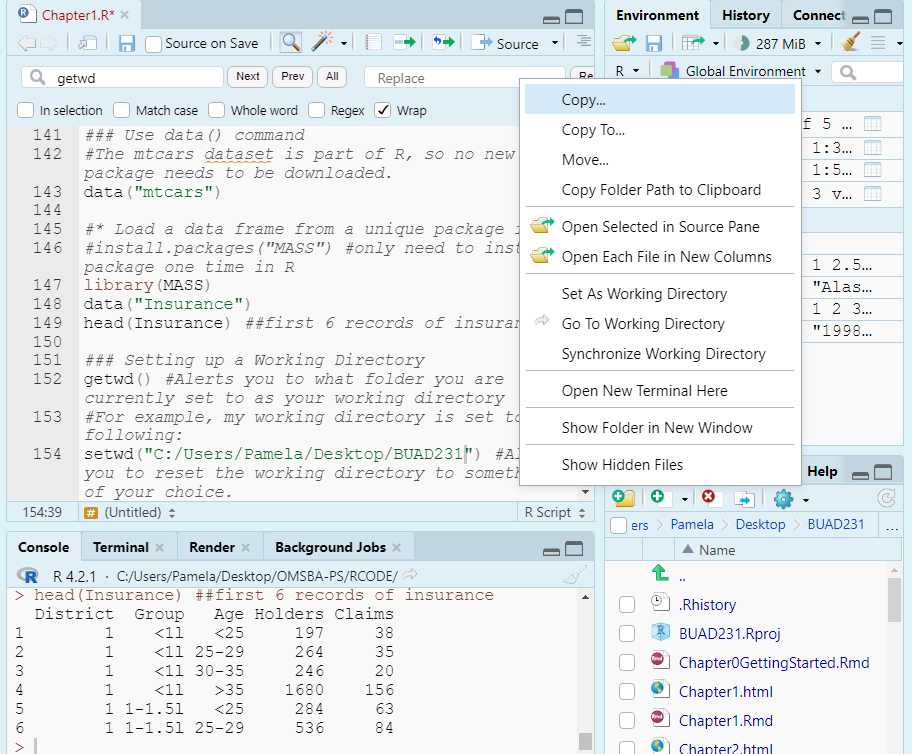
\includegraphics{Pictures/Ch1/WorkingDir.png}

}

\caption{Setting Your Working Directory}

\end{figure}%

\subsection{Reading in Data from .csv}\label{reading-in-data-from-.csv}

\begin{itemize}
\tightlist
\item
  Reading in a .csv file is extremely popular way to read in data.
\item
  There are a few functions to read in .csv files. And these functions
  would change based on the file type you are importing.
\end{itemize}

\subsubsection{read.csv() function}\label{read.csv-function}

\begin{verbatim}
 + Extremely popular way to read in data.
 + read.csv() is a base R function that comes built-in with R: No library necessary
\end{verbatim}

\begin{itemize}
\tightlist
\item
  All your datasets should be in a data folder in your working directory
  so that you and I have the same working directory.
\item
  Structure of function \emph{datasetName \textless-
  read.csv(``data/dataset.csv'')}
\end{itemize}

\begin{Shaded}
\begin{Highlighting}[]
\NormalTok{gss}\FloatTok{.2016} \OtherTok{\textless{}{-}} \FunctionTok{read.csv}\NormalTok{(}\AttributeTok{file =} \StringTok{"data/gss2016.csv"}\NormalTok{)}
\CommentTok{\# or equivalently}
\NormalTok{gss}\FloatTok{.2016} \OtherTok{\textless{}{-}} \FunctionTok{read.csv}\NormalTok{(}\StringTok{"data/gss2016.csv"}\NormalTok{)}
\CommentTok{\# Examine the contents of the file}
\FunctionTok{summary}\NormalTok{(}\AttributeTok{object =}\NormalTok{ gss}\FloatTok{.2016}\NormalTok{)}
\end{Highlighting}
\end{Shaded}

\begin{verbatim}
    grass               age           
 Length:2867        Length:2867       
 Class :character   Class :character  
 Mode  :character   Mode  :character  
\end{verbatim}

\begin{Shaded}
\begin{Highlighting}[]
\CommentTok{\# Or equivalently, we can shorten this to the following code}
\FunctionTok{summary}\NormalTok{(gss}\FloatTok{.2016}\NormalTok{)}
\end{Highlighting}
\end{Shaded}

\begin{verbatim}
    grass               age           
 Length:2867        Length:2867       
 Class :character   Class :character  
 Mode  :character   Mode  :character  
\end{verbatim}

\subsection{Using tidyverse to load
data}\label{using-tidyverse-to-load-data}

\subsubsection{read\_csv function}\label{read_csv-function}

\begin{itemize}
\tightlist
\item
  read\_csv() is a function from the readr package, which is part of the
  tidyverse ecosystem.
\item
  read\_csv() is generally faster than read.csv() as it's optimized for
  speed, making it more efficient, particularly for large datasets.
\end{itemize}

\begin{Shaded}
\begin{Highlighting}[]
\CommentTok{\# install.packages(tidyverse) \#\# Only need to install one time on}
\CommentTok{\# your computer. \#install.packages links have been commented out}
\CommentTok{\# during processing of RMarkdown.  Activate the library, which you}
\CommentTok{\# need to access each time you open R and RStudio}
\FunctionTok{library}\NormalTok{(tidyverse)}
\end{Highlighting}
\end{Shaded}

\begin{Shaded}
\begin{Highlighting}[]
\CommentTok{\# Now open the data file to evaluate with tidyverse}
\NormalTok{gss}\FloatTok{.2016}\NormalTok{b }\OtherTok{\textless{}{-}} \FunctionTok{read\_csv}\NormalTok{(}\AttributeTok{file =} \StringTok{"data/gss2016.csv"}\NormalTok{)}
\end{Highlighting}
\end{Shaded}

\section{Summarize Data}\label{summarize-data}

\begin{itemize}
\tightlist
\item
  Use the summary() function to examine the contents of the file.
\item
  The summary() function is part of base R and does not require a
  package.
\end{itemize}

\begin{Shaded}
\begin{Highlighting}[]
\FunctionTok{summary}\NormalTok{(}\AttributeTok{object =}\NormalTok{ gss}\FloatTok{.2016}\NormalTok{)}
\end{Highlighting}
\end{Shaded}

\begin{verbatim}
    grass               age           
 Length:2867        Length:2867       
 Class :character   Class :character  
 Mode  :character   Mode  :character  
\end{verbatim}

\begin{itemize}
\tightlist
\item
  Again, we can eliminate the object = because it is the first argument
  and is required.
\end{itemize}

\begin{Shaded}
\begin{Highlighting}[]
\FunctionTok{summary}\NormalTok{(gss}\FloatTok{.2016}\NormalTok{)}
\end{Highlighting}
\end{Shaded}

\begin{verbatim}
    grass               age           
 Length:2867        Length:2867       
 Class :character   Class :character  
 Mode  :character   Mode  :character  
\end{verbatim}

\subsection{Explicit Use of Libraries}\label{explicit-use-of-libraries}

\begin{itemize}
\item
  You can activate a library one time using library::function() format
\item
  For example, we can use the summarize() function from dplyr which is
  part of tidyverse installed earlier.
\item
  Since dplyr is part of tidyverse, there is actually no need to
  activate it when we have already activated tidyverse in this session,
  however, it does help when conflicts are present. More on that later.

  \begin{itemize}
  \tightlist
  \item
    The line below says to take the the gss.2016 data object and
    summarize the length of age using the dplyr library.
  \end{itemize}

\begin{Shaded}
\begin{Highlighting}[]
\NormalTok{dplyr}\SpecialCharTok{::}\FunctionTok{summarize}\NormalTok{(gss}\FloatTok{.2016}\NormalTok{, }\AttributeTok{length.age =} \FunctionTok{length}\NormalTok{(age))}
\end{Highlighting}
\end{Shaded}

\begin{verbatim}
  length.age
1       2867
\end{verbatim}
\item
  In the line of code above, we see package::function(). If we initiate
  the library like below, we do not need the beginning of the statement.
  The code below provides the same answer as the way written above.
\end{itemize}

\begin{Shaded}
\begin{Highlighting}[]
\FunctionTok{library}\NormalTok{(dplyr)}
\FunctionTok{summarize}\NormalTok{(gss}\FloatTok{.2016}\NormalTok{, }\AttributeTok{length.age =} \FunctionTok{length}\NormalTok{(age))}
\end{Highlighting}
\end{Shaded}

\begin{verbatim}
  length.age
1       2867
\end{verbatim}

\begin{itemize}
\tightlist
\item
  You try to access the ChickWeight dataset from the MASS package and
  summarize it generally using summary() and str() functions.
\item
  Earlier, we looked up the tapply() function in the help bar and found
  that the format is tapply(x, index, and fun), where x is a continuous
  variable, index is a grouping variable or factor, and fun is a
  function like mean. Use the tapply() function to take the mean weight
  of Chicks based on Diet. See the answer below.
\item
  While there are a few ways to get group means in R. I like the
  tapply() function which is used to apply a function over subsets of a
  vector. The function splits the data into subsets based on a given
  factor or factors, applies a specified function to each subset, and
  then returns the results in a convenient form. Here, we are applying
  the mean function.
\item
  To access a variable, use dataset\$variable or you can also attach a
  dataset to your code so you can just use the variable name later on.
  So use ChickWeight\$weight and ChickWeight\$Diet appropriately in the
  function alongside the FUN mean.
\end{itemize}

\begin{verbatim}
     weight           Time           Chick     Diet   
 Min.   : 35.0   Min.   : 0.00   13     : 12   1:220  
 1st Qu.: 63.0   1st Qu.: 4.00   9      : 12   2:120  
 Median :103.0   Median :10.00   20     : 12   3:120  
 Mean   :121.8   Mean   :10.72   10     : 12   4:118  
 3rd Qu.:163.8   3rd Qu.:16.00   17     : 12          
 Max.   :373.0   Max.   :21.00   19     : 12          
                                 (Other):506          
\end{verbatim}

\begin{verbatim}
       1        2        3        4 
102.6455 122.6167 142.9500 135.2627 
\end{verbatim}

\bookmarksetup{startatroot}

\chapter{Summary}\label{summary-1}

\begin{itemize}
\tightlist
\item
  In this lesson, we went over information to make sure you had some
  basics to really start learning R. There are a lot of ways to get the
  same things done in R; you have to find the way that works best for
  you. As we learn R, you will get used to doing things your way to be
  able to slice and evaluate the data to find rich information from the
  data sets we look at. As long as the data was handled properly, it
  does not matter how we reach our goal using R as long as we do it
  ourselves.
\end{itemize}

\bookmarksetup{startatroot}

\chapter{Descriptive Statistics}\label{descriptive-statistics}

\begin{itemize}
\tightlist
\item
  The goal of this lesson is to teach you how to summarize descriptive
  statistics for both quantitative and qualitative data in R. In order
  to succeed in this lesson, we need to learn how to describe data by
  understanding the difference between quantitative and qualitative data
  alongside examining its context. The context of the data gives us
  important information about how the data was collected, and its
  intended use.
\end{itemize}

\begin{Shaded}
\begin{Highlighting}[]
\DocumentationTok{\#\#\#\#\#\#\#\#\#\#\#\#\#\#\#\#\#\#\#\#\#\#\#\#\#\#\#\#\#\#\#\#\#\#\#\#}
\CommentTok{\# Project name: Descriptive Statistics}
\CommentTok{\# Data used: customers.csv}
\CommentTok{\# Libraries used: tidyverse, semTools}
\DocumentationTok{\#\#\#\#\#\#\#\#\#\#\#\#\#\#\#\#\#\#\#\#\#\#\#\#\#\#\#\#\#\#\#\#\#\#\#\#}
\end{Highlighting}
\end{Shaded}

\section{Lesson Objectives}\label{lesson-objectives-1}

\begin{itemize}
\tightlist
\item
  Choose and conduct descriptive analyses for categorical (factor)
  variables.
\item
  Choose and conduct descriptive analyses for continuous (numeric)
  variables.
\end{itemize}

\section{Consider While Reading}\label{consider-while-reading-1}

\begin{itemize}
\tightlist
\item
  In any analysis, it is critically important to understand your data
  set by evaluating descriptive statistics. For qualitative data, you
  should know how to calculate frequencies and proportions and make a
  user-friendly display of results. For quantitative data, you should
  know what a histogram is and how it is used to describe quantitative
  data. We also should know how to describe variables by their center
  and spread of the distribution.
\end{itemize}

\bookmarksetup{startatroot}

\chapter{Summarizing Qualitative
Data}\label{summarizing-qualitative-data}

\begin{itemize}
\tightlist
\item
  Qualitative data is information that cannot be easily counted,
  measured, or easily expressed using numbers.

  \begin{itemize}
  \tightlist
  \item
    Nominal variables: a type of categorical variable that represents
    discrete categories or groups with no inherent order or ranking

    \begin{itemize}
    \tightlist
    \item
      gender (male, female)
    \item
      marital status (single, married, divorced)
    \item
      eye color (blue, brown, green)
    \end{itemize}
  \item
    Ordinal variables: categories possess a natural order or ranking

    \begin{itemize}
    \tightlist
    \item
      a Likert scale measuring agreement with a statement (e.g.,
      strongly disagree, disagree, neutral, agree, strongly agree)
    \end{itemize}
  \end{itemize}
\item
  A frequency distribution shows the number of observations in each
  category for a factor or categorical variable.
\item
  Guidelines when constructing frequency distribution:

  \begin{itemize}
  \tightlist
  \item
    Classes or categories are mutually exclusive (they are all unique).
  \item
    Classes or categories are exhaustive (a full list of categories).
  \end{itemize}
\item
  To calculate frequencies, first, start with a variable that has
  categorical data.
\end{itemize}

\begin{Shaded}
\begin{Highlighting}[]
\CommentTok{\# Create a vector with some data that could be categorical}
\NormalTok{Sample\_Vector }\OtherTok{\textless{}{-}} \FunctionTok{c}\NormalTok{(}\StringTok{"A"}\NormalTok{, }\StringTok{"B"}\NormalTok{, }\StringTok{"A"}\NormalTok{, }\StringTok{"C"}\NormalTok{, }\StringTok{"A"}\NormalTok{, }\StringTok{"B"}\NormalTok{, }\StringTok{"A"}\NormalTok{, }\StringTok{"C"}\NormalTok{, }\StringTok{"A"}\NormalTok{, }\StringTok{"B"}\NormalTok{)}
\CommentTok{\# Create a data frame with the vector}
\NormalTok{data }\OtherTok{\textless{}{-}} \FunctionTok{data.frame}\NormalTok{(Sample\_Vector)}
\end{Highlighting}
\end{Shaded}

\begin{itemize}
\tightlist
\item
  To count the number of each category value, we can use the table()
  command.
\item
  The output shows a top row of categories and a bottom row that
  contains the number of observations in the category.
\end{itemize}

\begin{Shaded}
\begin{Highlighting}[]
\CommentTok{\# Create a table of frequencies}
\NormalTok{frequencies }\OtherTok{\textless{}{-}} \FunctionTok{table}\NormalTok{(data}\SpecialCharTok{$}\NormalTok{Sample\_Vector)}
\NormalTok{frequencies}
\end{Highlighting}
\end{Shaded}

\begin{verbatim}

A B C 
5 3 2 
\end{verbatim}

\begin{itemize}
\tightlist
\item
  Relative frequency is how often something happens divided by all
  outcomes.
\item
  The relative frequency is calculated by \(f_i/n\), where \(f_i\) is
  the frequency of class \(i\) and \(n\) is the total frequency.
\item
  We can use the prop.table() command to calculate relative frequency by
  dividing each category's frequency by the sample size.
\end{itemize}

\begin{Shaded}
\begin{Highlighting}[]
\CommentTok{\# Calculate proportions}
\NormalTok{proportions }\OtherTok{\textless{}{-}} \FunctionTok{prop.table}\NormalTok{(frequencies)}
\end{Highlighting}
\end{Shaded}

\begin{itemize}
\tightlist
\item
  The cumulative relative frequency is given by \(cf_i/n\), where
  \(cf_i\) is the cumulative frequency of class \(i\).
\item
  The cumsum() function calculates the cumulative distribution of the
  data
\end{itemize}

\begin{Shaded}
\begin{Highlighting}[]
\CommentTok{\# Calculate cumulative frequencies}
\NormalTok{cumulfreq }\OtherTok{\textless{}{-}} \FunctionTok{cumsum}\NormalTok{(frequencies)}
\CommentTok{\# Calculate cumulative proportions}
\NormalTok{cumulproportions }\OtherTok{\textless{}{-}} \FunctionTok{cumsum}\NormalTok{(}\FunctionTok{prop.table}\NormalTok{(frequencies))}
\end{Highlighting}
\end{Shaded}

\begin{itemize}
\tightlist
\item
  The rbind() function is used to combine multiple data frames or
  matrices by row. The name ``rbind'' stands for ``row bind''. Since the
  data produced by the table is in rows, we can use rbind to link them
  together.
\end{itemize}

\begin{Shaded}
\begin{Highlighting}[]
\CommentTok{\# combine into table}
\NormalTok{frequency\_table }\OtherTok{\textless{}{-}} \FunctionTok{rbind}\NormalTok{(frequencies, proportions, cumulfreq, cumulproportions)}
\CommentTok{\# Print the table}
\NormalTok{frequency\_table}
\end{Highlighting}
\end{Shaded}

\begin{verbatim}
                   A   B    C
frequencies      5.0 3.0  2.0
proportions      0.5 0.3  0.2
cumulfreq        5.0 8.0 10.0
cumulproportions 0.5 0.8  1.0
\end{verbatim}

\begin{itemize}
\tightlist
\item
  We can transpose a table using the t() command, which flips the
  dataset.
\end{itemize}

\begin{Shaded}
\begin{Highlighting}[]
\NormalTok{TransposedData }\OtherTok{\textless{}{-}} \FunctionTok{t}\NormalTok{(frequency\_table)}
\NormalTok{TransposedData}
\end{Highlighting}
\end{Shaded}

\begin{verbatim}
  frequencies proportions cumulfreq cumulproportions
A           5         0.5         5              0.5
B           3         0.3         8              0.8
C           2         0.2        10              1.0
\end{verbatim}

\begin{itemize}
\tightlist
\item
  Finally, sometimes we need to transform our calculations into a
  dataset.
\item
  The as.data.frame function is used to coerce or convert an object into
  a data frame
\end{itemize}

\begin{Shaded}
\begin{Highlighting}[]
\NormalTok{TransposedData }\OtherTok{\textless{}{-}} \FunctionTok{as.data.frame}\NormalTok{(TransposedData)}
\NormalTok{TransposedData}
\end{Highlighting}
\end{Shaded}

\begin{verbatim}
  frequencies proportions cumulfreq cumulproportions
A           5         0.5         5              0.5
B           3         0.3         8              0.8
C           2         0.2        10              1.0
\end{verbatim}

\bookmarksetup{startatroot}

\chapter{Summarizing Quantitative
Data}\label{summarizing-quantitative-data}

\section{Defining and Calculating Central
Tendency}\label{defining-and-calculating-central-tendency}

\begin{itemize}
\tightlist
\item
  The term central location refers to how numerical data tend to cluster
  around some middle or central value.
\item
  Measures of central location attempt to find a typical or central
  value that describes a variable.
\item
  Why frequency distributions do not work for numeric variables:

  \begin{itemize}
  \tightlist
  \item
    Numeric variables measured on a continuum.
  \item
    Instead, we calculate descriptive statistics including central
    tendency and spread of the values for a numeric variable.
  \end{itemize}
\item
  We will examine the three mostly widely used measures of central
  location: mean, median and mode.
\item
  Then we discuss a percentile: a measure of relative position.
\end{itemize}

\subsection{Using the Mean}\label{using-the-mean}

\begin{itemize}
\item
  The arithmetic mean or simply the mean is a primary measure of central
  location. It is often referred to as the average. Simply add up all
  the observations and divide by the number of observations.
\item
  The numerator (top of the fraction) is the sum (sigma) of all the
  values of x from the first value (i = 1) to the last value (n) divided
  by the number of values (n).
\item
  \(m_x = (\sum_{i=1}^{n} x_{i})/n\)
\item
  Consider the salaries of employees at a company:
  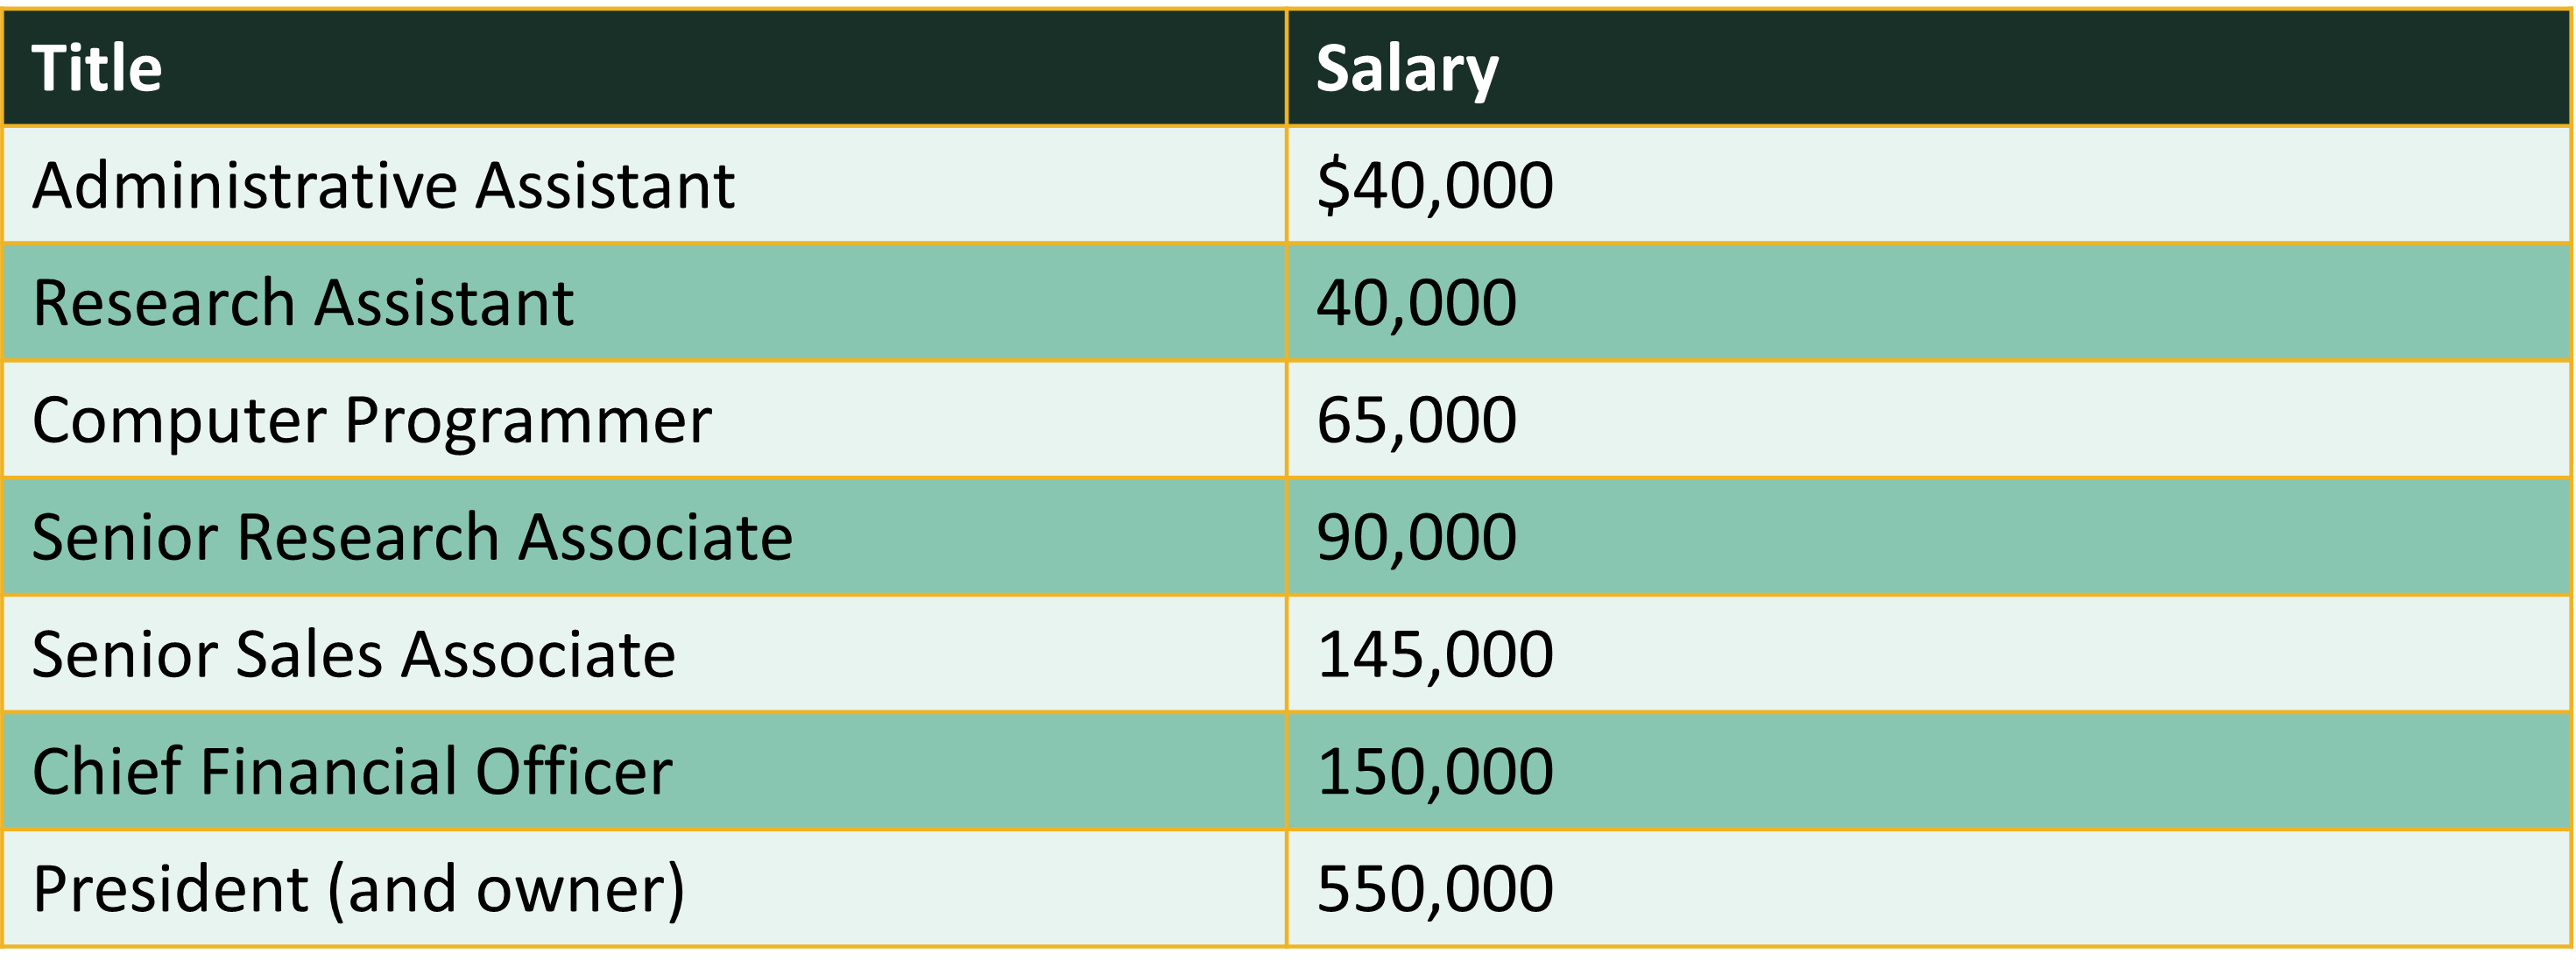
\includegraphics{Pictures/Ch2/Salaries.png}
\item
  We can use the mean() command to calculate the mean in R.
\end{itemize}

\begin{Shaded}
\begin{Highlighting}[]
\CommentTok{\# Create Vector of Salaries}
\NormalTok{salaries }\OtherTok{\textless{}{-}} \FunctionTok{c}\NormalTok{(}\DecValTok{40000}\NormalTok{, }\DecValTok{40000}\NormalTok{, }\DecValTok{65000}\NormalTok{, }\DecValTok{90000}\NormalTok{, }\DecValTok{145000}\NormalTok{, }\DecValTok{150000}\NormalTok{, }\DecValTok{550000}\NormalTok{)}
\CommentTok{\# Calculate the mean using the mean() command}
\FunctionTok{mean}\NormalTok{(salaries)}
\end{Highlighting}
\end{Shaded}

\begin{verbatim}
[1] 154285.7
\end{verbatim}

\begin{itemize}
\tightlist
\item
  Note that due to at least one \emph{outlier} this mean does not
  reflect the typical salary - more on that later.
\item
  If we edit our vector to include NAs, we have to account for this.
  This is a common way to handle NAs in functions that do not allow for
  them.
\end{itemize}

\begin{Shaded}
\begin{Highlighting}[]
\NormalTok{salaries2 }\OtherTok{\textless{}{-}} \FunctionTok{c}\NormalTok{(}\DecValTok{40000}\NormalTok{, }\DecValTok{40000}\NormalTok{, }\DecValTok{65000}\NormalTok{, }\DecValTok{90000}\NormalTok{, }\DecValTok{145000}\NormalTok{, }\DecValTok{150000}\NormalTok{, }\DecValTok{550000}\NormalTok{, }\ConstantTok{NA}\NormalTok{,}
    \ConstantTok{NA}\NormalTok{)}
\CommentTok{\# Calculate the mean using the mean() command Notice that it does not}
\CommentTok{\# work}
\FunctionTok{mean}\NormalTok{(salaries2)}
\end{Highlighting}
\end{Shaded}

\begin{verbatim}
[1] NA
\end{verbatim}

\begin{Shaded}
\begin{Highlighting}[]
\CommentTok{\# Add in na.rm parameter to get it to produce the mean with no NAs.}
\FunctionTok{mean}\NormalTok{(salaries2, }\AttributeTok{na.rm =} \ConstantTok{TRUE}\NormalTok{)}
\end{Highlighting}
\end{Shaded}

\begin{verbatim}
[1] 154285.7
\end{verbatim}

\begin{itemize}
\tightlist
\item
  Note that there are other types of means like the weighted mean or the
  geometric mean.\\
\item
  The weighted mean uses weights to determine the importance of each
  data point of a variable. It is calculated by
  \(\bar{x}_w = \frac{\sum_{i=1}^{n} w_i x_i}{\sum_{i=1}^{n} w_i}\),
  where are the weights associated to the values.
\item
  An example is below.
\end{itemize}

\begin{Shaded}
\begin{Highlighting}[]
\NormalTok{values }\OtherTok{\textless{}{-}} \FunctionTok{c}\NormalTok{(}\DecValTok{4}\NormalTok{, }\DecValTok{7}\NormalTok{, }\DecValTok{10}\NormalTok{, }\DecValTok{5}\NormalTok{, }\DecValTok{6}\NormalTok{)}
\NormalTok{weights }\OtherTok{\textless{}{-}} \FunctionTok{c}\NormalTok{(}\DecValTok{1}\NormalTok{, }\DecValTok{2}\NormalTok{, }\DecValTok{3}\NormalTok{, }\DecValTok{4}\NormalTok{, }\DecValTok{5}\NormalTok{)}
\NormalTok{weighted\_mean }\OtherTok{\textless{}{-}} \FunctionTok{weighted.mean}\NormalTok{(values, weights)}
\NormalTok{weighted\_mean}
\end{Highlighting}
\end{Shaded}

\begin{verbatim}
[1] 6.533333
\end{verbatim}

\subsection{Using the Median}\label{using-the-median}

\begin{itemize}
\tightlist
\item
  The median is another measure of central location that is not affected
  by outliers.
\item
  When the data are arranged in ascending order, the median is:

  \begin{itemize}
  \tightlist
  \item
    The middle value if the number of observations is odd, or
  \item
    The average of the two middle values if the number of observations
    is even.
  \end{itemize}
\item
  Consider the sorted salaries of employees presented earlier which
  contains an odd number of observations.\\
\item
  On the same salaries vector created above, use median() command to
  calculate the median in R.
\end{itemize}

\begin{Shaded}
\begin{Highlighting}[]
\CommentTok{\# Calculate the median using the median() command}
\FunctionTok{median}\NormalTok{(salaries)}
\end{Highlighting}
\end{Shaded}

\begin{verbatim}
[1] 90000
\end{verbatim}

\begin{itemize}
\tightlist
\item
  Now compare to the mean and note the large difference in numbers
  signifying that at least one outlier is most likely present.
\item
  Specifically, if the mean and median are different, it is likely the
  variable is skewed and contains outliers.
\end{itemize}

\begin{Shaded}
\begin{Highlighting}[]
\FunctionTok{mean}\NormalTok{(salaries)}
\end{Highlighting}
\end{Shaded}

\begin{verbatim}
[1] 154285.7
\end{verbatim}

\begin{itemize}
\tightlist
\item
  For another example, consider the sorted data below that contains an
  even number of values.
\end{itemize}

\begin{Shaded}
\begin{Highlighting}[]
\NormalTok{GrowthFund }\OtherTok{\textless{}{-}} \FunctionTok{c}\NormalTok{(}\SpecialCharTok{{-}}\FloatTok{38.32}\NormalTok{, }\FloatTok{1.71}\NormalTok{, }\FloatTok{3.17}\NormalTok{, }\FloatTok{5.99}\NormalTok{, }\FloatTok{12.56}\NormalTok{, }\FloatTok{13.47}\NormalTok{, }\FloatTok{16.89}\NormalTok{, }\FloatTok{16.96}\NormalTok{, }\FloatTok{32.16}\NormalTok{,}
    \FloatTok{36.29}\NormalTok{)}
\end{Highlighting}
\end{Shaded}

\begin{itemize}
\tightlist
\item
  When data contains an even number of values, the median is the average
  of the 2 sorted middle numbers (12.56 and 13.47).
\end{itemize}

\begin{Shaded}
\begin{Highlighting}[]
\FunctionTok{median}\NormalTok{(GrowthFund)}
\end{Highlighting}
\end{Shaded}

\begin{verbatim}
[1] 13.015
\end{verbatim}

\begin{Shaded}
\begin{Highlighting}[]
\NormalTok{(}\FloatTok{12.56} \SpecialCharTok{+} \FloatTok{13.47}\NormalTok{)}\SpecialCharTok{/}\DecValTok{2}
\end{Highlighting}
\end{Shaded}

\begin{verbatim}
[1] 13.015
\end{verbatim}

\begin{Shaded}
\begin{Highlighting}[]
\CommentTok{\# The mean is still the average}
\FunctionTok{mean}\NormalTok{(GrowthFund)}
\end{Highlighting}
\end{Shaded}

\begin{verbatim}
[1] 10.088
\end{verbatim}

\subsection{Using the Mode}\label{using-the-mode}

\begin{itemize}
\tightlist
\item
  The mode is another measure of central location.
\item
  The mode is the most frequently occurring value in a data set.
\item
  The mode is useful in summarizing categorical data.
\item
  A data set can have no mode, one mode (unimodal), two modes (bimodal)
  or many modes (multimodal).
\item
  The mode is less useful when there are more than three modes.
\item
  The mode is useful summary for a categorical variable.
\end{itemize}

\subsubsection{Example of Function with Salary
Variable}\label{example-of-function-with-salary-variable}

\begin{itemize}
\tightlist
\item
  Consider the salary of employees presented earlier. The mode is
  \$40,000 since this value appears most often.
\end{itemize}

\begin{Shaded}
\begin{Highlighting}[]
\CommentTok{\# Try this command with and without it.}
\FunctionTok{names}\NormalTok{(}\FunctionTok{sort}\NormalTok{(}\AttributeTok{x =} \FunctionTok{table}\NormalTok{(salaries), }\AttributeTok{decreasing =} \ConstantTok{TRUE}\NormalTok{))}
\end{Highlighting}
\end{Shaded}

\begin{verbatim}
[1] "40000"  "65000"  "90000"  "145000" "150000" "550000"
\end{verbatim}

\begin{itemize}
\tightlist
\item
  40,000 appears 2 times and is the mode because that occurs most often.
\end{itemize}

\subsubsection{Finding No Mode}\label{finding-no-mode}

\begin{itemize}
\tightlist
\item
  Look at the sort(table()) commands with the GrowthFund Vector we made
  earlier.
\item
  I added a {[}1:3{]} at the end of the statement to produce the 3
  highest frequencies found in the vector.
\end{itemize}

\begin{Shaded}
\begin{Highlighting}[]
\FunctionTok{sort}\NormalTok{(}\FunctionTok{table}\NormalTok{(GrowthFund), }\AttributeTok{decreasing =} \ConstantTok{TRUE}\NormalTok{)[}\DecValTok{1}\SpecialCharTok{:}\DecValTok{3}\NormalTok{]}
\end{Highlighting}
\end{Shaded}

\begin{verbatim}
GrowthFund
-38.32   1.71   3.17 
     1      1      1 
\end{verbatim}

\begin{itemize}
\tightlist
\item
  Even if you use this command, you still need to evaluate the data more
  systematically to verify the mode. If the highest frequency of the
  sorted table is 1, then there is no mode.
\end{itemize}

\bookmarksetup{startatroot}

\chapter{Defining and Calculating
Spread}\label{defining-and-calculating-spread}

\begin{itemize}
\tightlist
\item
  Spread is a measure of distance values are from the central value.
\item
  Each measure of central tendency has one or more corresponding
  measures of spread.
\item
  Mean: use variance or standard deviation to measure spread.

  \begin{itemize}
  \tightlist
  \item
    skewness and kurtosis help measure spread as well.
  \end{itemize}
\item
  Median: use range or interquartile range (IQR) to measure spread.
\item
  Mode: use the index of qualitative variation to measure spread.

  \begin{itemize}
  \tightlist
  \item
    Not formally testing here with a function.
  \end{itemize}
\end{itemize}

\section{Spread to Report with the
Mean}\label{spread-to-report-with-the-mean}

\subsection{Evaluating Skewness}\label{evaluating-skewness}

\begin{itemize}
\tightlist
\item
  Skewness is a measure of the extent to which a distribution is skewed.
\item
  Can evaluate skewness visually with histogram.

  \begin{itemize}
  \tightlist
  \item
    A histogram is a visual representation of a frequency or a relative
    frequency distribution.
  \item
    Bar height represents the respective class frequency (or relative
    frequency).
  \item
    Bar width represents the class width.
  \end{itemize}
\end{itemize}

\begin{figure}[H]

{\centering 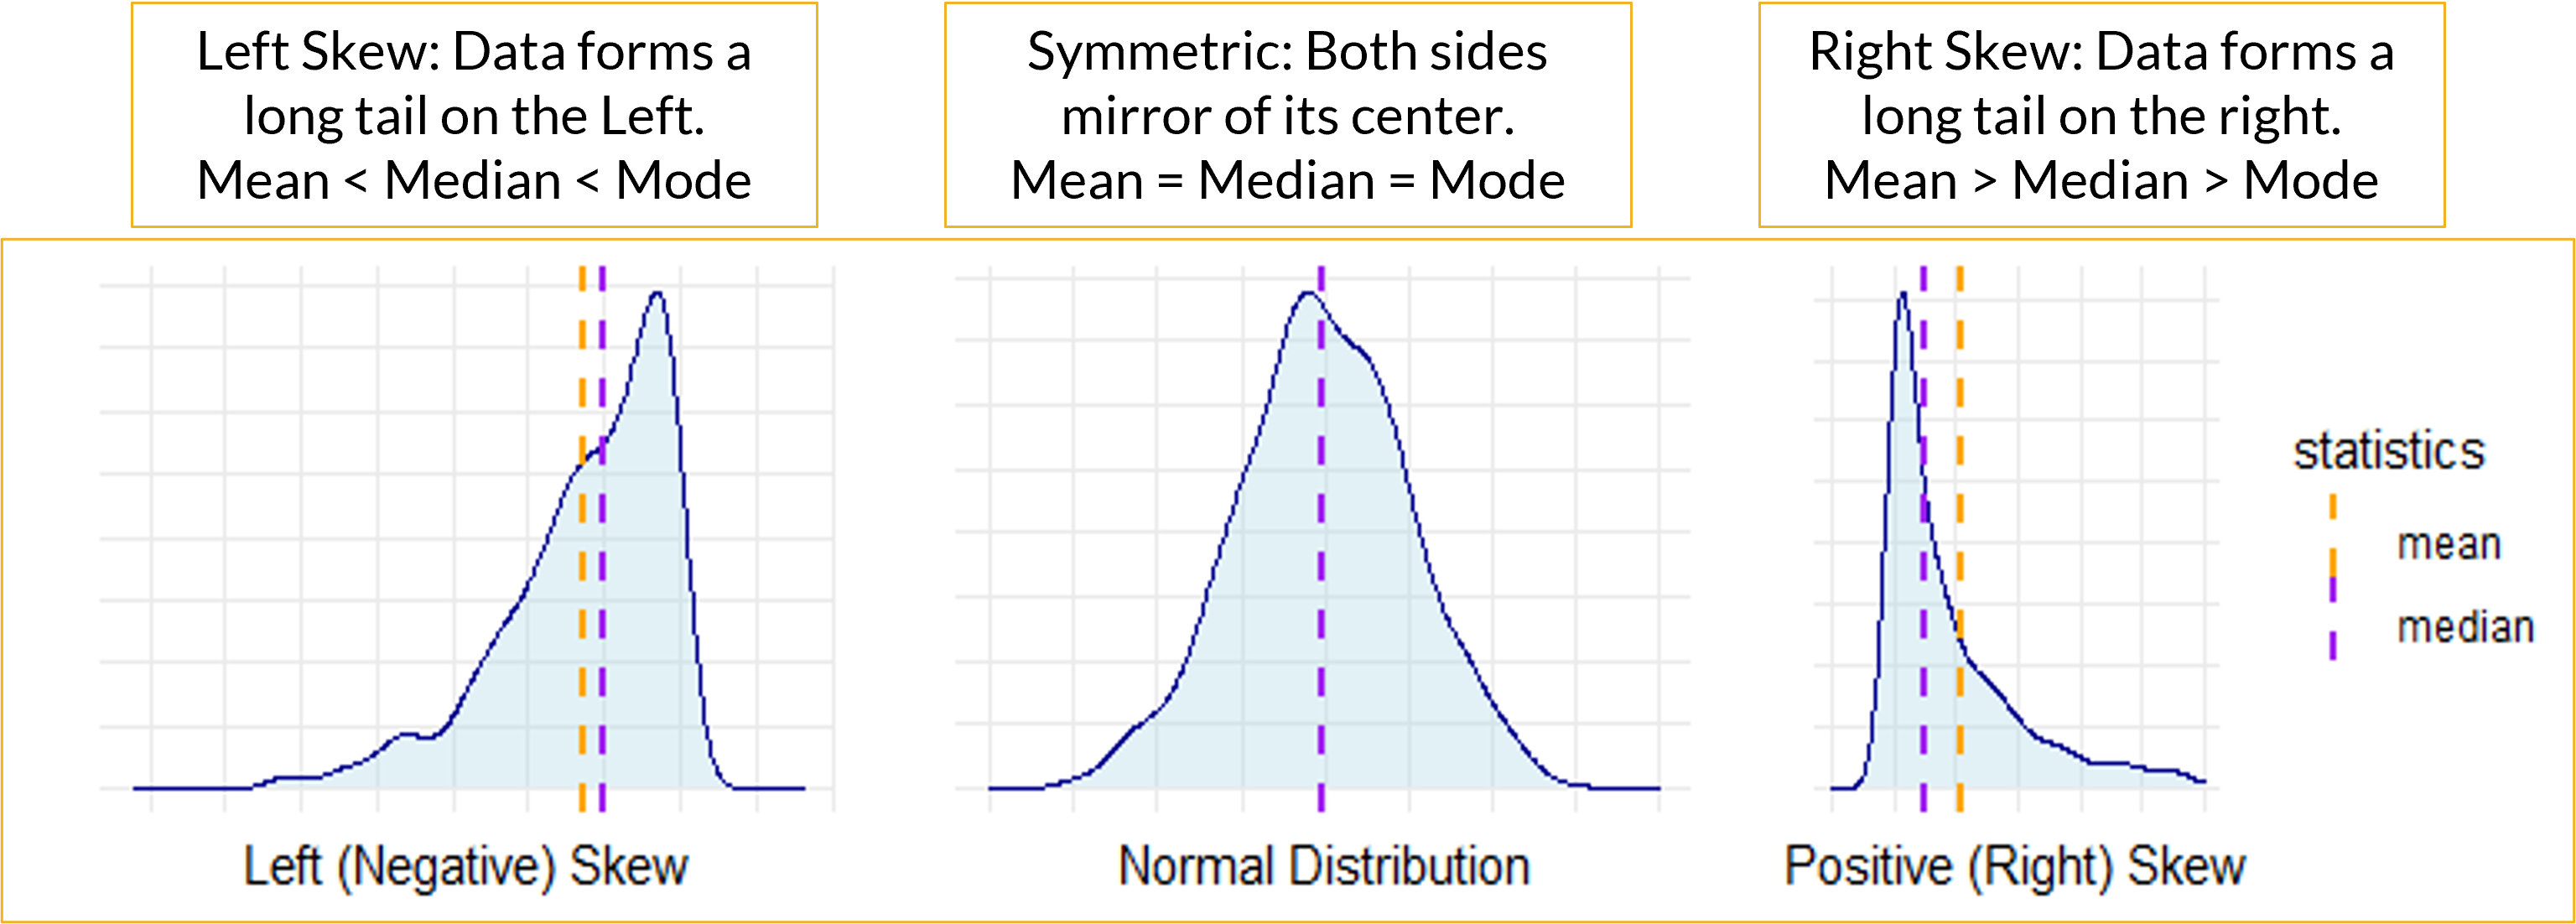
\includegraphics{Pictures/Ch2/Skewness.png}

}

\caption{Evaluating Skewness Visually}

\end{figure}%

\subsection{Skewed Distributions: Median Not Same as
Mean}\label{skewed-distributions-median-not-same-as-mean}

\begin{itemize}
\tightlist
\item
  Sometimes, a histogram is difficult to tell if skewness is present or
  if the data is relatively normal or symmetric.
\item
  If Mean is less than Median and Mode, then the variable is
  Left-Skewed.
\item
  If the Mean is greater than the Median and Mode, then the variable is
  Right-Skewed.
\item
  If the Mean is about equal to the Median and Mode, then the variable
  has a symmetric distribution.
\item
  In R, we can easily look at mean and median with the summary()
  command.
\end{itemize}

\begin{figure}[H]

{\centering 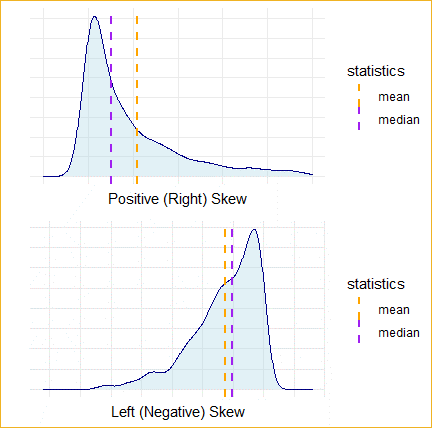
\includegraphics{Pictures/Ch2/SkewMeanMedian.png}

}

\caption{Evaluating Skewness Using Mean and Median}

\end{figure}%

\begin{itemize}
\tightlist
\item
  Mean is great when data are normally distributed (data is not skewed).
\item
  Mean is not a good representation of skewed data where outliers are
  present.

  \begin{itemize}
  \tightlist
  \item
    Adding together a set of values that includes a few very large or
    very small values like those on the far left of a left-skewed
    distribution or the far right of the right-skewed distribution will
    result in a large or small total value in the numerator of Equation
    and therefore the mean will be a large or small value relative to
    the actual middle of the data.
  \end{itemize}
\end{itemize}

\subsection{Using skew() Command in R}\label{using-skew-command-in-r}

\begin{itemize}
\tightlist
\item
  The skew() command is from the semTools package. The
  install.packages() command is commented out below, but install it one
  time on your R before commenting it out.
\end{itemize}

\begin{Shaded}
\begin{Highlighting}[]
\CommentTok{\# install the semTools package if necessary.}
\CommentTok{\# install.packages(\textquotesingle{}semTools\textquotesingle{}) Activate the library}
\FunctionTok{library}\NormalTok{(semTools)}
\end{Highlighting}
\end{Shaded}

\begin{itemize}
\tightlist
\item
  After the package is installed and loaded, run the skew() command on
  the salaries vector made above.
\end{itemize}

\begin{Shaded}
\begin{Highlighting}[]
\FunctionTok{skew}\NormalTok{(salaries)}
\end{Highlighting}
\end{Shaded}

\begin{verbatim}
 skew (g1)         se          z          p 
2.31126775 0.92582010 2.49645450 0.01254418 
\end{verbatim}

\subsection{Interpreting the skew() Command
Results}\label{interpreting-the-skew-command-results}

\begin{itemize}
\item
  se = standard error
\item
  z = skew/se
\item
  If the sample size is small (n \textless{} 50), z values outside the
  --2 to 2 range are a problem.
\item
  If the sample size is between 50 and 300, z values outside the --3.29
  to 3.29 range are a problem.
\item
  For large samples (n \textgreater{} 300), using a visual is
  recommended over the statistics, but generally z values outside the
  range of --7 to 7 can be considered problematic.
\item
  Salary: Our sample size was small, \textless50, so the z value of
  2.496 in regards to the salary vector indicates there is a problem
  with skewness.
\item
  GrowthFund: We can check the skew of GrowthFund.
\end{itemize}

\begin{Shaded}
\begin{Highlighting}[]
\FunctionTok{skew}\NormalTok{(GrowthFund)}
\end{Highlighting}
\end{Shaded}

\begin{verbatim}
  skew (g1)          se           z           p 
-1.38071963  0.77459667 -1.78250137  0.07466751 
\end{verbatim}

\begin{itemize}
\tightlist
\item
  GrowthFund was also considered a small sample size, so the same -2/2
  thresholds are used. Here, our z value is -1.78250137, which is in
  normal range. This indicates there is no problem with skewness.
\end{itemize}

\section{Histograms}\label{histograms}

\begin{itemize}
\tightlist
\item
  A histogram is a graphical representation of the distribution of
  numerical data.
\item
  It consists of a series of contiguous rectangles, or bars, where the
  area of each bar corresponds to the frequency of observations within a
  particular range or bin of values.
\item
  The x-axis typically represents the range of values being measured,
  while the y-axis represents the frequency or count of observations
  falling within each range.
\item
  Histograms are commonly used in statistics and data analysis to
  visualize the distribution of a dataset and identify patterns or
  trends.
\item
  They are particularly useful for understanding the central tendency,
  variability, and shape of the data distribution - this includes our
  observation of skewness.
\item
  Works much better with larger datsets.
\end{itemize}

\subsection{Commands to Make a
Histogram}\label{commands-to-make-a-histogram}

\begin{itemize}
\item
  hist() command in base R.
\item
  geom\_histogram() command in ggplot2 package.
\item
  a hist using the GrowthFund dataset does not look that great because
  its sample size is so small.
\end{itemize}

\begin{Shaded}
\begin{Highlighting}[]
\FunctionTok{hist}\NormalTok{(GrowthFund)}
\end{Highlighting}
\end{Shaded}

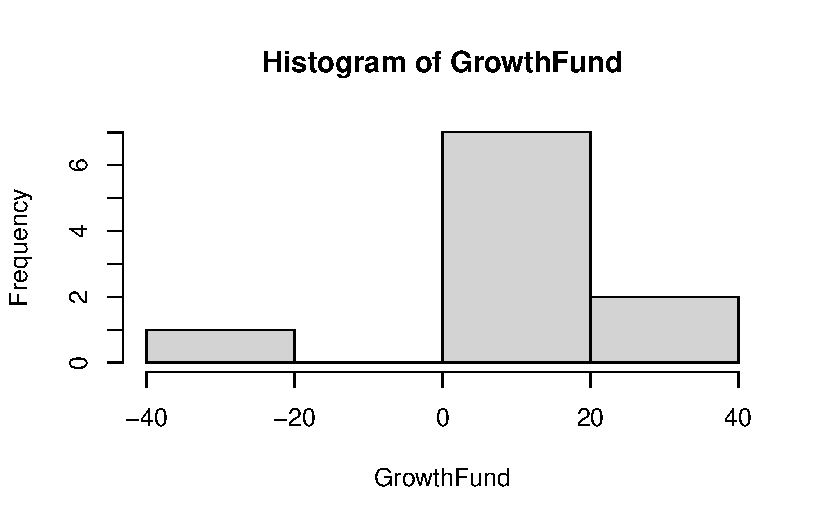
\includegraphics{descriptives_files/figure-pdf/unnamed-chunk-21-1.pdf}

\subsection{hist vs geom\_histogram}\label{hist-vs-geom_histogram}

\begin{itemize}
\tightlist
\item
  In R, hist() and geom\_histogram() are both used to create histograms,
  but they belong to different packages and have slightly different
  functionalities.
\end{itemize}

\begin{Shaded}
\begin{Highlighting}[]
\CommentTok{\# Making an appropriate data.frame to use the hist() command}
\NormalTok{HousePrice }\OtherTok{\textless{}{-}} \FunctionTok{c}\NormalTok{(}\DecValTok{430}\NormalTok{, }\DecValTok{520}\NormalTok{, }\DecValTok{460}\NormalTok{, }\DecValTok{475}\NormalTok{, }\DecValTok{670}\NormalTok{, }\DecValTok{521}\NormalTok{, }\DecValTok{670}\NormalTok{, }\DecValTok{417}\NormalTok{, }\DecValTok{533}\NormalTok{, }\DecValTok{525}\NormalTok{, }\DecValTok{538}\NormalTok{,}
    \DecValTok{370}\NormalTok{, }\DecValTok{530}\NormalTok{, }\DecValTok{525}\NormalTok{, }\DecValTok{430}\NormalTok{, }\DecValTok{330}\NormalTok{, }\DecValTok{575}\NormalTok{, }\DecValTok{555}\NormalTok{, }\DecValTok{521}\NormalTok{, }\DecValTok{350}\NormalTok{, }\DecValTok{399}\NormalTok{, }\DecValTok{560}\NormalTok{, }\DecValTok{440}\NormalTok{, }\DecValTok{425}\NormalTok{, }\DecValTok{669}\NormalTok{,}
    \DecValTok{660}\NormalTok{, }\DecValTok{702}\NormalTok{, }\DecValTok{540}\NormalTok{, }\DecValTok{460}\NormalTok{, }\DecValTok{588}\NormalTok{, }\DecValTok{445}\NormalTok{, }\DecValTok{412}\NormalTok{, }\DecValTok{735}\NormalTok{, }\DecValTok{537}\NormalTok{, }\DecValTok{630}\NormalTok{, }\DecValTok{430}\NormalTok{)}
\NormalTok{HousePrice }\OtherTok{\textless{}{-}} \FunctionTok{data.frame}\NormalTok{(HousePrice)}
\end{Highlighting}
\end{Shaded}

\begin{itemize}
\tightlist
\item
  hist(): This function is from the base R graphics package and is used
  to create histograms. It provides a simple way to visualize the
  distribution of a single variable.
\end{itemize}

\begin{Shaded}
\begin{Highlighting}[]
\CommentTok{\# Using base R to create the histogram.}
\FunctionTok{hist}\NormalTok{(HousePrice}\SpecialCharTok{$}\NormalTok{HousePrice, }\AttributeTok{breaks =} \DecValTok{5}\NormalTok{, }\AttributeTok{main =} \StringTok{"A Histogram"}\NormalTok{, }\AttributeTok{xlab =} \StringTok{"House Prices (in $1,000s)"}\NormalTok{,}
    \AttributeTok{col =} \StringTok{"yellow"}\NormalTok{)}
\end{Highlighting}
\end{Shaded}

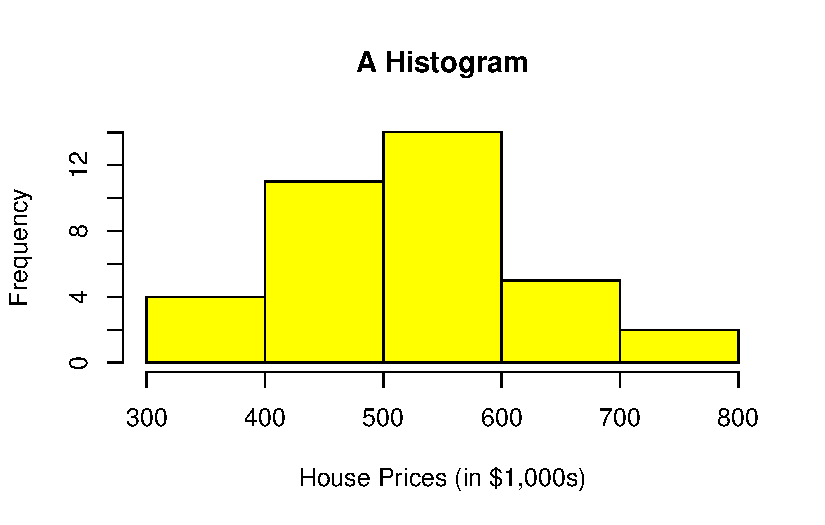
\includegraphics{descriptives_files/figure-pdf/unnamed-chunk-23-1.pdf}

\begin{Shaded}
\begin{Highlighting}[]
\FunctionTok{library}\NormalTok{(tidyverse)}
\end{Highlighting}
\end{Shaded}

\begin{itemize}
\tightlist
\item
  geom\_histogram(): This function is from the ggplot2 package, which is
  part of the tidyverse. It is used to create histograms as part of a
  more flexible and powerful plotting system.
\end{itemize}

\begin{Shaded}
\begin{Highlighting}[]
\CommentTok{\# Using geom\_histogram() command to create the histogram.}
\FunctionTok{ggplot}\NormalTok{(HousePrice, }\FunctionTok{aes}\NormalTok{(}\AttributeTok{x =}\NormalTok{ HousePrice)) }\SpecialCharTok{+} \FunctionTok{geom\_histogram}\NormalTok{(}\AttributeTok{binwidth =} \DecValTok{100}\NormalTok{,}
    \AttributeTok{boundary =} \DecValTok{300}\NormalTok{, }\AttributeTok{color =} \StringTok{"black"}\NormalTok{, }\AttributeTok{fill =} \StringTok{"yellow"}\NormalTok{) }\SpecialCharTok{+} \FunctionTok{labs}\NormalTok{(}\AttributeTok{title =} \StringTok{"A Histogram"}\NormalTok{,}
    \AttributeTok{x =} \StringTok{"House Prices (in $1,000s)"}\NormalTok{, }\AttributeTok{y =} \StringTok{"Frequency"}\NormalTok{)}
\end{Highlighting}
\end{Shaded}

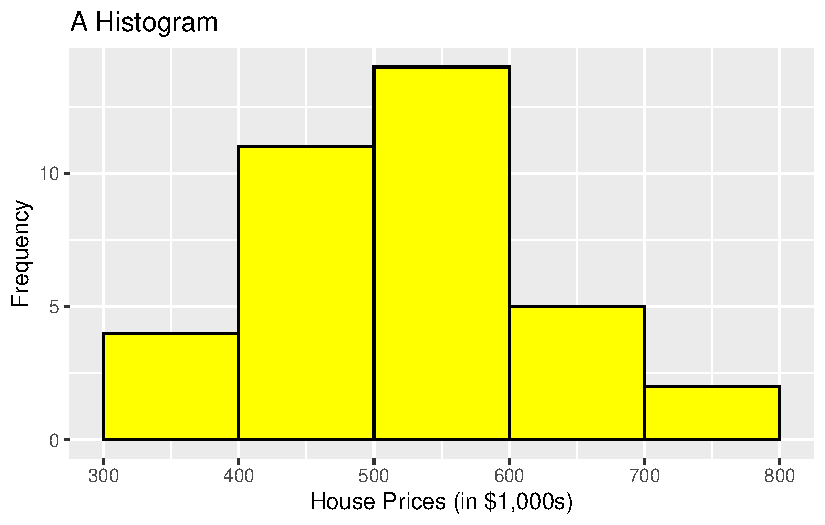
\includegraphics{descriptives_files/figure-pdf/unnamed-chunk-25-1.pdf}

\begin{itemize}
\item
  We could add more parameters here to make the 2 histograms look
  identical, but this configuration of parameters is very close. Take
  note that there are a lot more parameters you can add to the
  geom\_histogram() command than you can with base R to make it look
  more professional. Be sure to look them up and also check with the
  notes in the book, which focuses on geom\_histogram instead of hist().
\item
  Variance is a measure of spread for numeric variables that is
  essentially the average of the squared differences between each
  observation value on some variable and the mean for that variable with
  population variance.
  \[Population Var(X) = \sigma^2 = \sum{(x_i-\mu)^2}/N\]
  \[Sample Var(x) = s^2 = \sum{(x_i-\bar{x})^2}/(n-1)\]
\item
  Standard deviation is the square root of the variance.

  \begin{itemize}
  \tightlist
  \item
    Use var() command and sd() command to calculate sample variance and
    sample standard deviation.
  \end{itemize}
\end{itemize}

\begin{Shaded}
\begin{Highlighting}[]
\DocumentationTok{\#\# Calculated from Small Sample}
\NormalTok{x }\OtherTok{\textless{}{-}} \FunctionTok{c}\NormalTok{(}\DecValTok{1}\NormalTok{, }\DecValTok{2}\NormalTok{, }\DecValTok{3}\NormalTok{, }\DecValTok{4}\NormalTok{, }\DecValTok{5}\NormalTok{)}
\FunctionTok{sum}\NormalTok{((x }\SpecialCharTok{{-}} \FunctionTok{mean}\NormalTok{(x))}\SpecialCharTok{\^{}}\DecValTok{2}\SpecialCharTok{/}\NormalTok{(}\DecValTok{5} \SpecialCharTok{{-}} \DecValTok{1}\NormalTok{))}
\end{Highlighting}
\end{Shaded}

\begin{verbatim}
[1] 2.5
\end{verbatim}

\begin{Shaded}
\begin{Highlighting}[]
\FunctionTok{var}\NormalTok{(x)}
\end{Highlighting}
\end{Shaded}

\begin{verbatim}
[1] 2.5
\end{verbatim}

\begin{Shaded}
\begin{Highlighting}[]
\FunctionTok{sqrt}\NormalTok{(}\FunctionTok{var}\NormalTok{(x))}
\end{Highlighting}
\end{Shaded}

\begin{verbatim}
[1] 1.581139
\end{verbatim}

\begin{Shaded}
\begin{Highlighting}[]
\FunctionTok{sd}\NormalTok{(x)}
\end{Highlighting}
\end{Shaded}

\begin{verbatim}
[1] 1.581139
\end{verbatim}

\begin{Shaded}
\begin{Highlighting}[]
\FunctionTok{sd}\NormalTok{(HousePrice}\SpecialCharTok{$}\NormalTok{HousePrice)}
\end{Highlighting}
\end{Shaded}

\begin{verbatim}
[1] 102.6059
\end{verbatim}

\begin{Shaded}
\begin{Highlighting}[]
\FunctionTok{var}\NormalTok{(HousePrice}\SpecialCharTok{$}\NormalTok{HousePrice)}
\end{Highlighting}
\end{Shaded}

\begin{verbatim}
[1] 10527.97
\end{verbatim}

\begin{itemize}
\tightlist
\item
  Looking at Spread for a Larger Dataset
\end{itemize}

\begin{Shaded}
\begin{Highlighting}[]
\NormalTok{customers }\OtherTok{\textless{}{-}} \FunctionTok{read.csv}\NormalTok{(}\StringTok{"data/customers.csv"}\NormalTok{)}
\FunctionTok{summary}\NormalTok{(customers}\SpecialCharTok{$}\NormalTok{Spending, }\AttributeTok{na.rm =} \ConstantTok{TRUE}\NormalTok{)  }\CommentTok{\#mean and median}
\end{Highlighting}
\end{Shaded}

\begin{verbatim}
   Min. 1st Qu.  Median    Mean 3rd Qu.    Max. 
   50.0   383.8   662.0   659.6   962.2  1250.0 
\end{verbatim}

\begin{Shaded}
\begin{Highlighting}[]
\DocumentationTok{\#\#\# Spread to Report with the Mean}
\FunctionTok{sd}\NormalTok{(customers}\SpecialCharTok{$}\NormalTok{Spending, }\AttributeTok{na.rm =} \ConstantTok{TRUE}\NormalTok{)}
\end{Highlighting}
\end{Shaded}

\begin{verbatim}
[1] 350.2876
\end{verbatim}

\begin{Shaded}
\begin{Highlighting}[]
\FunctionTok{var}\NormalTok{(customers}\SpecialCharTok{$}\NormalTok{Spending, }\AttributeTok{na.rm =} \ConstantTok{TRUE}\NormalTok{)}
\end{Highlighting}
\end{Shaded}

\begin{verbatim}
[1] 122701.4
\end{verbatim}

\subsection{Kurtosis in Evaluating Mean
Spread}\label{kurtosis-in-evaluating-mean-spread}

\begin{itemize}
\tightlist
\item
  Kurtosis is the sharpness of the peak of a frequency-distribution
  curve or more formally a measure of how many observations are in the
  tails of a distribution.
\item
  A normal distribution will have a kurtosis value of three;

  \begin{itemize}
  \tightlist
  \item
    Distributions with kurtosis around 3 are described as mesokurtic.
  \item
    If kurtosis is significantly above or below 3, there is excess
    kurtosis.

    \begin{itemize}
    \tightlist
    \item
      Values of kurtosis significantly above 3 indicate the distribution
      is leptokurtic, with fewer observations in the tails than a normal
      distribution (the fewer observations in the tails often give a
      distribution a pointy look).
    \item
      Values of kurtosis significantly below 3 indicate the distribution
      is platykurtic, with more observations in the tails than a normal
      distribution would have given the mean, standard deviation, and
      sample size.
    \end{itemize}
  \item
    Uses kurtosis() command from the semTools package.
  \end{itemize}
\end{itemize}

\begin{figure}[H]

{\centering 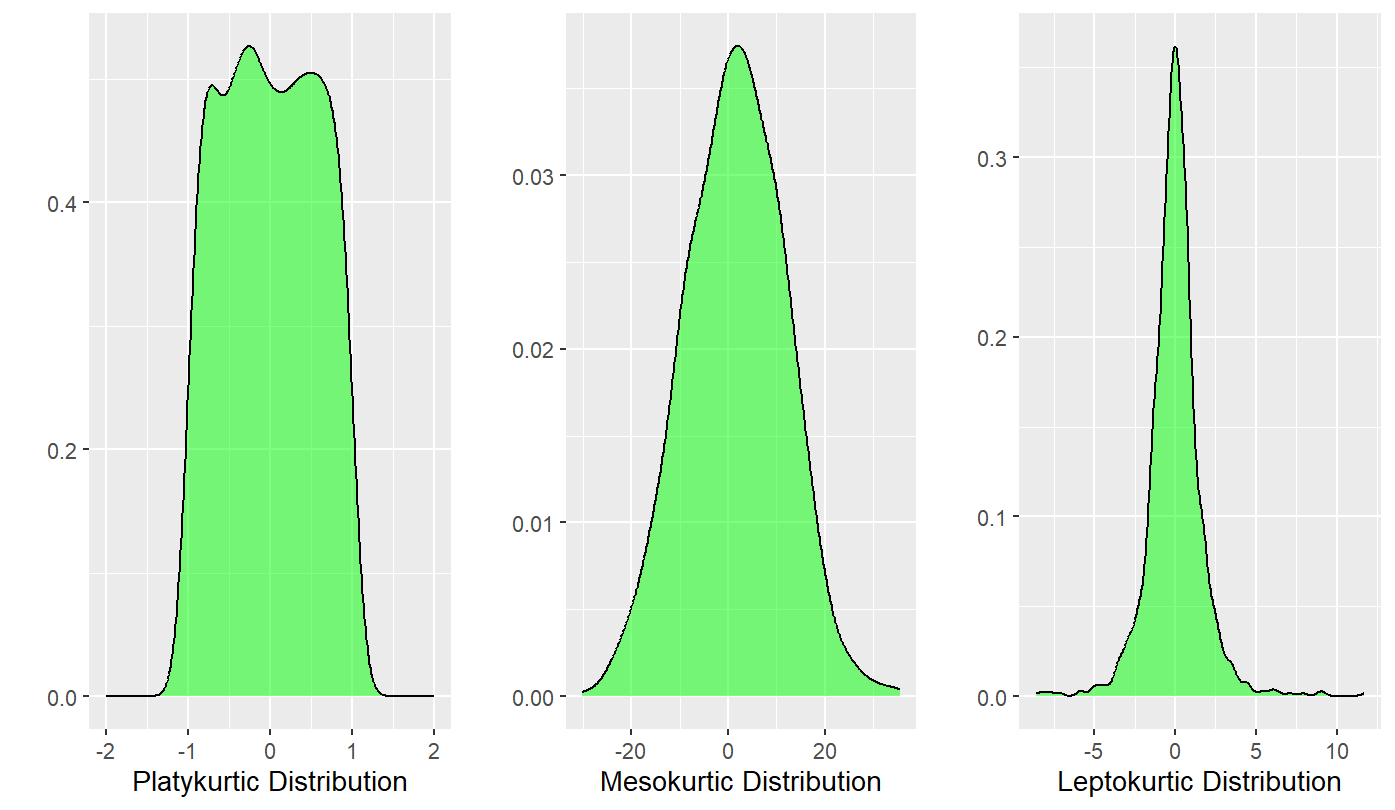
\includegraphics{Pictures/Ch2/Kurtosis.png}

}

\caption{Evaluate Kurtosis}

\end{figure}%

\begin{itemize}
\tightlist
\item
  The kurtosis() command subtracts 3 from the kurtosis, so positive
  values will be indicative to a leptokurtic distribution and negative
  will indicate a platykurtic distribution. To see if kurtosis
  (leptokurtic or platykurtic) is significant, we confirm them by first
  evaluating the z-score to see if the variable is normal or not. The
  same cutoff values from skew also apply for the z for small, medium,
  and large sample sizes in kurtosis. These are the same basic rules for
  the rules in judging skewness.
\end{itemize}

\begin{Shaded}
\begin{Highlighting}[]
\CommentTok{\# z{-}value is 3.0398, which is \textgreater{} 2 indicating leptokurtic Small sample}
\CommentTok{\# size: range is {-}2 to 2}
\FunctionTok{kurtosis}\NormalTok{(salaries)}
\end{Highlighting}
\end{Shaded}

\begin{verbatim}
Excess Kur (g2)              se               z               p 
    5.628711065     1.851640200     3.039851407     0.002366949 
\end{verbatim}

\begin{Shaded}
\begin{Highlighting}[]
\CommentTok{\# z{-}value is 2.20528007, which is \textgreater{} 2 indicating leptokurtic Small}
\CommentTok{\# sample size: range is {-}2 to 2}
\FunctionTok{kurtosis}\NormalTok{(GrowthFund)}
\end{Highlighting}
\end{Shaded}

\begin{verbatim}
Excess Kur (g2)              se               z               p 
     3.41640519      1.54919334      2.20528007      0.02743445 
\end{verbatim}

\begin{Shaded}
\begin{Highlighting}[]
\CommentTok{\# Small sample size: range is {-}2 to 2 Skewness and kurtosis are both}
\CommentTok{\# in range.}
\FunctionTok{skew}\NormalTok{(HousePrice}\SpecialCharTok{$}\NormalTok{HousePrice)  }\CommentTok{\#normal}
\end{Highlighting}
\end{Shaded}

\begin{verbatim}
skew (g1)        se         z         p 
0.3173182 0.4082483 0.7772676 0.4370009 
\end{verbatim}

\begin{Shaded}
\begin{Highlighting}[]
\FunctionTok{kurtosis}\NormalTok{(HousePrice}\SpecialCharTok{$}\NormalTok{HousePrice)  }\CommentTok{\#normal}
\end{Highlighting}
\end{Shaded}

\begin{verbatim}
Excess Kur (g2)              se               z               p 
     -0.5399982       0.8164966      -0.6613601       0.5083814 
\end{verbatim}

\begin{itemize}
\tightlist
\item
  The rules of determining problematic distributions with regards to
  kurtosis are below.

  \begin{itemize}
  \tightlist
  \item
    If the sample size is small (n \textless{} 50), z values outside the
    --2 to 2 range are a problem.
  \item
    If the sample size is between 50 and 300, z values outside the
    --3.29 to 3.29 range are a problem.
  \item
    For large samples (n \textgreater{} 300), using a visual is
    recommended over the statistics, but generally z values outside the
    range of --7 to 7 can be considered problematic.
  \item
    If kurtosis is found, then evaluate the excess kur score to see if
    it is positive or negative to determine whether it is leptokurtic or
    platykurtic.
  \end{itemize}
\item
  Let's do a few more examples using the customers dataset.
\end{itemize}

\begin{Shaded}
\begin{Highlighting}[]
\CommentTok{\# Noted sample size at 200 observations or a medium sample size.}
\CommentTok{\# Using threshold –3.29 to 3.29 to assess normality.}

\CommentTok{\#{-}3.4245446445 is below {-}3.29 so kurtosis is present}
\CommentTok{\# Negative kurtosis value indicates platykurtic}
\FunctionTok{kurtosis}\NormalTok{(customers}\SpecialCharTok{$}\NormalTok{Spending)}
\end{Highlighting}
\end{Shaded}

\begin{verbatim}
Excess Kur (g2)              se               z               p 
  -1.1862970634    0.3464101615   -3.4245446445    0.0006158307 
\end{verbatim}

\begin{Shaded}
\begin{Highlighting}[]
\CommentTok{\# Normal: 2.977622119 is in between {-}3.29 and 3.29}
\FunctionTok{kurtosis}\NormalTok{(customers}\SpecialCharTok{$}\NormalTok{Income)}
\end{Highlighting}
\end{Shaded}

\begin{verbatim}
Excess Kur (g2)              se               z               p 
    1.031478559     0.346410162     2.977622119     0.002904939 
\end{verbatim}

\begin{Shaded}
\begin{Highlighting}[]
\CommentTok{\#{-}3.7251961028 is below {-}3.29 so kurtosis is present}
\CommentTok{\# Negative kurtosis value indicates platykurtic}
\FunctionTok{kurtosis}\NormalTok{(customers}\SpecialCharTok{$}\NormalTok{HHSize)}
\end{Highlighting}
\end{Shaded}

\begin{verbatim}
Excess Kur (g2)              se               z               p 
  -1.2904457837    0.3464101615   -3.7251961028    0.0001951634 
\end{verbatim}

\begin{Shaded}
\begin{Highlighting}[]
\CommentTok{\# Normal: {-}0.20056607 is in between {-}3.29 and 3.29}
\FunctionTok{kurtosis}\NormalTok{(customers}\SpecialCharTok{$}\NormalTok{Orders)}
\end{Highlighting}
\end{Shaded}

\begin{verbatim}
Excess Kur (g2)              se               z               p 
    -0.06947812      0.34641016     -0.20056607      0.84103789 
\end{verbatim}

\section{Spread to Report with the
Median}\label{spread-to-report-with-the-median}

\begin{itemize}
\tightlist
\item
  Range = Maximum Value -- Minimum Value.

  \begin{itemize}
  \tightlist
  \item
    Simplest measure.
  \item
    Focuses on Extreme values.
  \item
    Use commands diff(range()) or max() -- min().
  \end{itemize}
\item
  IQR: Difference between the first and third quartiles.

  \begin{itemize}
  \tightlist
  \item
    Use IQR() command or quantile() command.
  \end{itemize}
\end{itemize}

\begin{Shaded}
\begin{Highlighting}[]
\FunctionTok{summary}\NormalTok{(customers}\SpecialCharTok{$}\NormalTok{Spending, }\AttributeTok{na.rm =} \ConstantTok{TRUE}\NormalTok{)}
\end{Highlighting}
\end{Shaded}

\begin{verbatim}
   Min. 1st Qu.  Median    Mean 3rd Qu.    Max. 
   50.0   383.8   662.0   659.6   962.2  1250.0 
\end{verbatim}

\begin{Shaded}
\begin{Highlighting}[]
\FunctionTok{diff}\NormalTok{(}\FunctionTok{range}\NormalTok{(customers}\SpecialCharTok{$}\NormalTok{Spending, }\AttributeTok{na.rm =} \ConstantTok{TRUE}\NormalTok{))}
\end{Highlighting}
\end{Shaded}

\begin{verbatim}
[1] 1200
\end{verbatim}

\begin{Shaded}
\begin{Highlighting}[]
\FunctionTok{max}\NormalTok{(customers}\SpecialCharTok{$}\NormalTok{Spending, }\AttributeTok{na.rm =} \ConstantTok{TRUE}\NormalTok{) }\SpecialCharTok{{-}} \FunctionTok{min}\NormalTok{(customers}\SpecialCharTok{$}\NormalTok{Spending, }\AttributeTok{na.rm =} \ConstantTok{TRUE}\NormalTok{)}
\end{Highlighting}
\end{Shaded}

\begin{verbatim}
[1] 1200
\end{verbatim}

\begin{Shaded}
\begin{Highlighting}[]
\FunctionTok{IQR}\NormalTok{(customers}\SpecialCharTok{$}\NormalTok{Spending, }\AttributeTok{na.rm =} \ConstantTok{TRUE}\NormalTok{)}
\end{Highlighting}
\end{Shaded}

\begin{verbatim}
[1] 578.5
\end{verbatim}

\section{Spread to Report with the
Mode}\label{spread-to-report-with-the-mode}

\begin{itemize}
\tightlist
\item
  While there is no great function to test for spread, you can look at
  the data and see if it is concentrated around 1 or 2 frequencies. If
  it is, then the spread is distorted towards those high frequency
  values.
\end{itemize}

\bookmarksetup{startatroot}

\chapter{Summary}\label{summary-2}

\begin{itemize}
\tightlist
\item
  In this lesson, we worked through descriptive statistics including
  skewness and kurtosis. We learned about variables and scales of
  measurement, how to summarize qualitative and quantitative data.
\end{itemize}

\bookmarksetup{startatroot}

\chapter{Data Preparation}\label{data-preparation}

\begin{itemize}
\tightlist
\item
  The goal of this lesson is to teach you how to clean datasets for use
  in analytics. This lesson focuses on dplyr. dplyr is a package in R
  that provides a set of functions for data manipulation tasks. These
  functions are designed to be intuitive and efficient, making it easier
  to work with data frames or tibbles (a modern reimagining of data
  frames provided by the tibble package).
\end{itemize}

\begin{Shaded}
\begin{Highlighting}[]
\DocumentationTok{\#\#\#\#\#\#\#\#\#\#\#\#\#\#\#\#\#\#\#\#\#\#\#\#\#\#\#\#\#\#\#\#\#\#\#\#}
\CommentTok{\# Project name: Data Preparation}
\CommentTok{\# Data used: gss.2016, brfss.csv, customers.csv, gig.csv from Blackboard, iris from datasets}
\CommentTok{\# Libraries used: tidyverse, semTools, lubridate}
\DocumentationTok{\#\#\#\#\#\#\#\#\#\#\#\#\#\#\#\#\#\#\#\#\#\#\#\#\#\#\#\#\#\#\#\#\#\#\#\#}
\end{Highlighting}
\end{Shaded}

\section{At a Glance}\label{at-a-glance-1}

\begin{itemize}
\tightlist
\item
  In order to succeed in this lesson, we need to be able to evaluate
  variables and understand how to clean and prepare data to make
  variables easier to use and in the correct form. This sometimes
  includes subsetting and filtering data alongside other techniques.
\end{itemize}

\section{Lesson Objectives}\label{lesson-objectives-2}

\begin{itemize}
\tightlist
\item
  Create variables and identify and change data types.
\item
  Learn how to clean data via dplyr.
\end{itemize}

\section{Consider While Reading}\label{consider-while-reading-2}

\begin{itemize}
\tightlist
\item
  We often spend a considerable amount of time inspecting and preparing
  the data for the subsequent analysis. This includes the following:

  \begin{itemize}
  \tightlist
  \item
    Evaluating Data Types
  \item
    Sorting Data
  \item
    Selecting Variables
  \item
    Filtering Data
  \item
    Counting Data
  \item
    Handling Missing Values
  \item
    Summarizing
  \item
    Grouping Data
  \end{itemize}
\end{itemize}

\bookmarksetup{startatroot}

\chapter{Evaluating Data Types}\label{evaluating-data-types}

\begin{itemize}
\tightlist
\item
  There are a number of data types in R that are common to programming
  and statistical analysis.
\item
  A data type of a variable specifies the type of data that is stored
  inside that variable. Sometimes when you read in data it is in the
  correct type, and other times, you need to force it into the type you
  need to conduct the analysis. In this section, we are going to go over
  the following data types.\\
\end{itemize}

\begin{enumerate}
\def\labelenumi{\arabic{enumi}.}
\tightlist
\item
  Factor data type:

  \begin{itemize}
  \tightlist
  \item
    Ordinal: Contain categories that have some logical order
    (e.g.~categories of age).
  \item
    Nominal: Have categories that have no logical order (e.g., religious
    affiliation and marital status).
  \end{itemize}
\end{enumerate}

\begin{itemize}
\tightlist
\item
  R will treat each unique value of a factor as a different level.
\end{itemize}

Ordinal Variable * Ordinal data may be categorized and ranked with
respect to some characteristic or trait. * For example, instructors are
often evaluated on an ordinal scale (excellent, good, fair, poor). *
This scale allows us to code the data based on order, assuming equal
distance between scale items (aka likert items). * You can make an
ordinal factor data type in R, or you can convert the order to
meaningful numbers. This is typically done with survey items where an
excellent to poor = 1, 2, 3, 4 respectively.

\begin{Shaded}
\begin{Highlighting}[]
\CommentTok{\# Take a vector representing evaluation scores, named evaluate}
\NormalTok{evaluate }\OtherTok{\textless{}{-}} \FunctionTok{c}\NormalTok{(}\StringTok{"excellent"}\NormalTok{, }\StringTok{"good"}\NormalTok{, }\StringTok{"fair"}\NormalTok{, }\StringTok{"poor"}\NormalTok{, }\StringTok{"excellent"}\NormalTok{, }\StringTok{"good"}\NormalTok{)}
\CommentTok{\# We can use a series of ifelse() commands to change the data to}
\CommentTok{\# numerical.}
\NormalTok{evalNumerical }\OtherTok{\textless{}{-}} \FunctionTok{ifelse}\NormalTok{(evaluate }\SpecialCharTok{==} \StringTok{"excellent"}\NormalTok{, }\DecValTok{4}\NormalTok{, }\FunctionTok{ifelse}\NormalTok{(evaluate }\SpecialCharTok{==}
    \StringTok{"good"}\NormalTok{, }\DecValTok{3}\NormalTok{, }\FunctionTok{ifelse}\NormalTok{(evaluate }\SpecialCharTok{==} \StringTok{"fair"}\NormalTok{, }\DecValTok{2}\NormalTok{, }\DecValTok{1}\NormalTok{)))}
\NormalTok{evalNumerical}
\end{Highlighting}
\end{Shaded}

\begin{verbatim}
[1] 4 3 2 1 4 3
\end{verbatim}

Nominal Variable * With nominal variables, data are simply categories
for grouping. * For example, coding race/ethnicity might have a category
value of White, Black, Native American, Asian/Pacific Islander, Other. *
Qualitative values may be converted to quantitative values for analysis
purposes. + White = 1, Black = 2, etc. This conversion to numerical
representation of the category would be needed to run some analysis. +
Sometimes, R does this on our behalf depending on commands used. * We
can force a variable into a factor data type using the as.factor()
command. * If we use the read.csv() command, we can sometimes do this by
setting an argument \(stringsAsFactors=TRUE\). We will do this later in
the lesson.

\begin{enumerate}
\def\labelenumi{\arabic{enumi}.}
\setcounter{enumi}{1}
\tightlist
\item
  Numerical data types: A Vector of Numbers (Real or Integer)
\end{enumerate}

\begin{itemize}
\item
  Continuous (Real) variables can take any value along some continuum,
  hence continuous.

  \begin{itemize}
  \tightlist
  \item
    We can force a variable into a numerical data type by using the
    as.numeric() command.
  \item
    For example, we could collect information on a participants age,
    height, weight, or distance traveled.
  \end{itemize}
\item
  Two ways to create:

  \begin{itemize}
  \tightlist
  \item
    We can also create a numeric variable by ensuring our value we
    assign is a number!
  \item
    We can force a variable into an real number data type by using the
    as.numeric() command.
  \end{itemize}

\begin{Shaded}
\begin{Highlighting}[]
\CommentTok{\# Assign Rhode Island limit for medical marijuana in ounces per}
\CommentTok{\# person}
\NormalTok{kOuncesRhode }\OtherTok{\textless{}{-}} \FloatTok{2.5}
\CommentTok{\# Identify the data type}
\FunctionTok{class}\NormalTok{(}\AttributeTok{x =}\NormalTok{ kOuncesRhode)}
\end{Highlighting}
\end{Shaded}

\begin{verbatim}
[1] "numeric"
\end{verbatim}
\item
  Discrete (Integer) Variables:

  \begin{itemize}
  \tightlist
  \item
    Discrete variables can only take a countable number of distinct
    values.
  \item
    We can force a variable into an integer data type by using the
    as.integer() command.
  \end{itemize}
\item
  For example, we could collect information on the number of children in
  a family or number of points scored in a basketball game.
\end{itemize}

\begin{Shaded}
\begin{Highlighting}[]
\CommentTok{\# Assign the value of 4 to a constant called kTestInteger and set as}
\CommentTok{\# an integer}
\NormalTok{kTestInteger }\OtherTok{\textless{}{-}} \FunctionTok{as.integer}\NormalTok{(}\DecValTok{4}\NormalTok{)}
\FunctionTok{class}\NormalTok{(kTestInteger)  }\CommentTok{\#Confirm the data type is an integer }
\end{Highlighting}
\end{Shaded}

\begin{verbatim}
[1] "integer"
\end{verbatim}

\begin{Shaded}
\begin{Highlighting}[]
\CommentTok{\# Use as.integer() to truncate the variable ouncesRhode}
\NormalTok{Trunc }\OtherTok{\textless{}{-}} \FunctionTok{as.integer}\NormalTok{(kOuncesRhode)}
\NormalTok{Trunc}
\end{Highlighting}
\end{Shaded}

\begin{verbatim}
[1] 2
\end{verbatim}

\begin{enumerate}
\def\labelenumi{\arabic{enumi}.}
\setcounter{enumi}{2}
\tightlist
\item
  Character data type: Wrapped in either single or double quotation
  marks.

  \begin{itemize}
  \tightlist
  \item
    Includes letters, words, or numbers that cannot logically be
    included in calculations (e.g., a zip code).
  \item
    A quick example is below that shows how to assign a character value
    to a variable.
  \end{itemize}
\end{enumerate}

\begin{Shaded}
\begin{Highlighting}[]
\CommentTok{\# Make constants}
\NormalTok{kFirstName }\OtherTok{\textless{}{-}} \StringTok{"Corina"}
\NormalTok{kLastName }\OtherTok{\textless{}{-}} \StringTok{"Hughes"}
\CommentTok{\# Check the data type}
\FunctionTok{class}\NormalTok{(}\AttributeTok{x =}\NormalTok{ kFirstName)}
\end{Highlighting}
\end{Shaded}

\begin{verbatim}
[1] "character"
\end{verbatim}

\begin{Shaded}
\begin{Highlighting}[]
\CommentTok{\# Create a zip code constant and check the data type}
\NormalTok{kZipCode }\OtherTok{\textless{}{-}} \StringTok{"97405"}
\FunctionTok{class}\NormalTok{(}\AttributeTok{x =}\NormalTok{ kZipCode)}
\end{Highlighting}
\end{Shaded}

\begin{verbatim}
[1] "character"
\end{verbatim}

\begin{enumerate}
\def\labelenumi{\arabic{enumi}.}
\setcounter{enumi}{3}
\tightlist
\item
  Logical data type: Values of TRUE and FALSE
\end{enumerate}

\begin{itemize}
\item
  Result of some expression.

  \begin{itemize}
  \tightlist
  \item
    A quick example is below that shows how to assign a logical value to
    a variable.
  \end{itemize}

\begin{Shaded}
\begin{Highlighting}[]
\CommentTok{\# Store the result of 6 \textgreater{} 8 in a constant called kSixEight}
\NormalTok{kSixEight }\OtherTok{\textless{}{-}} \DecValTok{6} \SpecialCharTok{\textgreater{}} \DecValTok{8}
\CommentTok{\# Can use comparison tests with the following == \textgreater{}= \textless{}= \textgreater{} \textless{} \textless{}\textgreater{} !=}
\NormalTok{kSixEight  }\CommentTok{\# Print kSixEight}
\end{Highlighting}
\end{Shaded}

\begin{verbatim}
[1] FALSE
\end{verbatim}

\begin{Shaded}
\begin{Highlighting}[]
\CommentTok{\# Determine the data type of kSixEight}
\FunctionTok{class}\NormalTok{(}\AttributeTok{x =}\NormalTok{ kSixEight)}
\end{Highlighting}
\end{Shaded}

\begin{verbatim}
[1] "logical"
\end{verbatim}
\end{itemize}

\begin{enumerate}
\def\labelenumi{\arabic{enumi}.}
\setcounter{enumi}{4}
\tightlist
\item
  Date data type: A variable that should be a date.
\end{enumerate}

\begin{Shaded}
\begin{Highlighting}[]
\CommentTok{\# Convert date info in format \textquotesingle{}mm/dd/yyyy\textquotesingle{} using as.Date}
\NormalTok{strDates }\OtherTok{\textless{}{-}} \FunctionTok{c}\NormalTok{(}\StringTok{"01/05/1965"}\NormalTok{, }\StringTok{"08/16/1975"}\NormalTok{)}
\NormalTok{dates }\OtherTok{\textless{}{-}} \FunctionTok{as.Date}\NormalTok{(strDates, }\StringTok{"\%m/\%d/\%Y"}\NormalTok{)}
\FunctionTok{str}\NormalTok{(dates)}
\end{Highlighting}
\end{Shaded}

\begin{verbatim}
 Date[1:2], format: "1965-01-05" "1975-08-16"
\end{verbatim}

\begin{itemize}
\tightlist
\item
  lubridate is a package specifically for converting dates. This package
  makes dates a lot easier to work with.
\end{itemize}

\begin{Shaded}
\begin{Highlighting}[]
\CommentTok{\# Convert date info in format \textquotesingle{}mm/dd/yyyy\textquotesingle{} using lubridate}
\FunctionTok{library}\NormalTok{(lubridate)}
\NormalTok{strDates }\OtherTok{\textless{}{-}} \FunctionTok{c}\NormalTok{(}\StringTok{"01/05/1965"}\NormalTok{, }\StringTok{"08/16/1975"}\NormalTok{)}
\NormalTok{dates }\OtherTok{\textless{}{-}} \FunctionTok{mdy}\NormalTok{(strDates)}
\FunctionTok{str}\NormalTok{(dates)}
\end{Highlighting}
\end{Shaded}

\begin{verbatim}
 Date[1:2], format: "1965-01-05" "1975-08-16"
\end{verbatim}

\begin{itemize}
\tightlist
\item
  If you are only given a year and a month, you can use the ym() command
  to turn it to a date. But take note that it will add a day to the
  value as a placeholder.
\end{itemize}

\begin{Shaded}
\begin{Highlighting}[]
\CommentTok{\# Convert date info in format \textquotesingle{}yyyymm\textquotesingle{} using lubridate}
\NormalTok{stryyyymm }\OtherTok{\textless{}{-}} \FunctionTok{c}\NormalTok{(}\StringTok{"202201"}\NormalTok{, }\StringTok{"202003"}\NormalTok{, }\StringTok{"202204"}\NormalTok{)}
\NormalTok{dates }\OtherTok{\textless{}{-}} \FunctionTok{ym}\NormalTok{(stryyyymm)}
\FunctionTok{str}\NormalTok{(dates)}
\end{Highlighting}
\end{Shaded}

\begin{verbatim}
 Date[1:3], format: "2022-01-01" "2020-03-01" "2022-04-01"
\end{verbatim}

\section{Nominal Example with
Dataset}\label{nominal-example-with-dataset}

\begin{Shaded}
\begin{Highlighting}[]
\FunctionTok{library}\NormalTok{(tidyverse)}
\NormalTok{gss}\FloatTok{.2016} \OtherTok{\textless{}{-}} \FunctionTok{read\_csv}\NormalTok{(}\AttributeTok{file =} \StringTok{"data/gss2016.csv"}\NormalTok{)}
\end{Highlighting}
\end{Shaded}

\begin{Shaded}
\begin{Highlighting}[]
\CommentTok{\# Examine the variable types with summary and class functions.}
\FunctionTok{summary}\NormalTok{(gss}\FloatTok{.2016}\NormalTok{)}
\end{Highlighting}
\end{Shaded}

\begin{verbatim}
    grass               age           
 Length:2867        Length:2867       
 Class :character   Class :character  
 Mode  :character   Mode  :character  
\end{verbatim}

\begin{Shaded}
\begin{Highlighting}[]
\FunctionTok{class}\NormalTok{(gss}\FloatTok{.2016}\SpecialCharTok{$}\NormalTok{grass)  }\CommentTok{\#Check the data type.}
\end{Highlighting}
\end{Shaded}

\begin{verbatim}
[1] "character"
\end{verbatim}

\begin{Shaded}
\begin{Highlighting}[]
\NormalTok{gss}\FloatTok{.2016}\SpecialCharTok{$}\NormalTok{grass }\OtherTok{\textless{}{-}} \FunctionTok{as.factor}\NormalTok{(gss}\FloatTok{.2016}\SpecialCharTok{$}\NormalTok{grass)  }\CommentTok{\#Turn to a factor.}
\FunctionTok{class}\NormalTok{(gss}\FloatTok{.2016}\SpecialCharTok{$}\NormalTok{grass)  }\CommentTok{\#Confirming it is now correct.}
\end{Highlighting}
\end{Shaded}

\begin{verbatim}
[1] "factor"
\end{verbatim}

\section{Numerical Example with
Dataset}\label{numerical-example-with-dataset}

\begin{itemize}
\tightlist
\item
  We need to ensure data can be coded as numeric before using the
  as.numeric() command. For example, to handle the variable age, it
  seems like numerical values except one value of ``89 OR OLDER''. If
  as.numeric() command was used on this variable, it would put all the
  89 and older observations as NAs. To force it to be a numerical
  variable, and keep that the sample participants were the oldest value,
  we need to recode it and then use the as.numeric() command to coerce
  it into a number.
\item
  Recoding the 89 and older to 89 does cause the data to lack integrity
  in its current form because it will treat the people over 89 years old
  as 89. But, we are limited here because this needs to be a numerical
  variable for us to proceed. We will learn a step later on in this
  section to transform the age variable into categories so that we bring
  back our data integrity.
\end{itemize}

\begin{Shaded}
\begin{Highlighting}[]
\FunctionTok{class}\NormalTok{(gss}\FloatTok{.2016}\SpecialCharTok{$}\NormalTok{age)}
\end{Highlighting}
\end{Shaded}

\begin{verbatim}
[1] "character"
\end{verbatim}

\begin{Shaded}
\begin{Highlighting}[]
\CommentTok{\# Recode \textquotesingle{}89 OR OLDER\textquotesingle{} into just \textquotesingle{}89\textquotesingle{}}
\NormalTok{gss}\FloatTok{.2016}\SpecialCharTok{$}\NormalTok{age }\OtherTok{\textless{}{-}} \FunctionTok{recode}\NormalTok{(gss}\FloatTok{.2016}\SpecialCharTok{$}\NormalTok{age, }\StringTok{\textasciigrave{}}\AttributeTok{89 OR OLDER}\StringTok{\textasciigrave{}} \OtherTok{=} \StringTok{"89"}\NormalTok{)}
\CommentTok{\# Convert to numeric data type}
\NormalTok{gss}\FloatTok{.2016}\SpecialCharTok{$}\NormalTok{age }\OtherTok{\textless{}{-}} \FunctionTok{as.numeric}\NormalTok{(gss}\FloatTok{.2016}\SpecialCharTok{$}\NormalTok{age)}
\FunctionTok{summary}\NormalTok{(gss}\FloatTok{.2016}\NormalTok{)  }\CommentTok{\#Conduct final check confirming correct data types}
\end{Highlighting}
\end{Shaded}

\begin{verbatim}
       grass           age       
 DK       : 110   Min.   :18.00  
 IAP      : 911   1st Qu.:34.00  
 LEGAL    :1126   Median :49.00  
 NOT LEGAL: 717   Mean   :49.16  
 NA's     :   3   3rd Qu.:62.00  
                  Max.   :89.00  
                  NA's   :10     
\end{verbatim}

\bookmarksetup{startatroot}

\chapter{Arrange}\label{arrange}

\begin{itemize}
\tightlist
\item
  Sorting or arranging the dataset allows you to specify an order based
  on variable values.
\item
  Sorting allows us to review the range of values for each variable, and
  we can sort based on a single or multiple variables.
\item
  Notice the difference between sort() and arrange() functions below.

  \begin{itemize}
  \tightlist
  \item
    The sort() function sorts a vector.
  \item
    The arrange() function sorts a dataset based on a variable.
  \end{itemize}
\item
  To conduct an example, read in the data set called gig.csv from your
  working directory.
\end{itemize}

\begin{Shaded}
\begin{Highlighting}[]
\NormalTok{gig }\OtherTok{\textless{}{-}} \FunctionTok{read.csv}\NormalTok{(}\StringTok{"data/gig.csv"}\NormalTok{, }\AttributeTok{stringsAsFactors =} \ConstantTok{TRUE}\NormalTok{, }\AttributeTok{na.strings =} \StringTok{""}\NormalTok{)}
\FunctionTok{dim}\NormalTok{(gig)}
\end{Highlighting}
\end{Shaded}

\begin{verbatim}
[1] 604   4
\end{verbatim}

\begin{Shaded}
\begin{Highlighting}[]
\FunctionTok{head}\NormalTok{(gig)}
\end{Highlighting}
\end{Shaded}

\begin{verbatim}
  EmployeeID  Wage     Industry        Job
1          1 32.81 Construction    Analyst
2          2 46.00   Automotive   Engineer
3          3 43.13 Construction  Sales Rep
4          4 48.09   Automotive      Other
5          5 43.62   Automotive Accountant
6          6 46.98 Construction   Engineer
\end{verbatim}

\begin{itemize}
\item
  Using the arrange() function, we add the dataset, followed by a comma
  and then add in the variable we want to sort. This arranges from small
  to large.
\item
  Below is code to rearrange data based on Wage and save it in a new
  object.
\end{itemize}

\begin{Shaded}
\begin{Highlighting}[]
\NormalTok{sortTidy }\OtherTok{\textless{}{-}} \FunctionTok{arrange}\NormalTok{(gig, Wage)}
\FunctionTok{head}\NormalTok{(sortTidy)}
\end{Highlighting}
\end{Shaded}

\begin{verbatim}
  EmployeeID  Wage     Industry        Job
1        467 24.28 Construction   Engineer
2        547 24.28 Construction  Sales Rep
3        580 24.28 Construction Accountant
4        559 24.42 Construction   Engineer
5         16 24.76   Automotive Programmer
6        221 24.76   Automotive Programmer
\end{verbatim}

\begin{itemize}
\tightlist
\item
  We can apply a desc() function inside the arrange function to re-sort
  from high to low like shown below.
\end{itemize}

\begin{Shaded}
\begin{Highlighting}[]
\NormalTok{sortTidyDesc }\OtherTok{\textless{}{-}} \FunctionTok{arrange}\NormalTok{(gig, }\FunctionTok{desc}\NormalTok{(Wage))}
\FunctionTok{head}\NormalTok{(sortTidyDesc)}
\end{Highlighting}
\end{Shaded}

\begin{verbatim}
  EmployeeID  Wage     Industry        Job
1        110 51.00 Construction      Other
2         79 50.00   Automotive   Engineer
3        348 49.91 Construction Accountant
4        373 49.91 Construction Accountant
5        599 49.84   Automotive   Engineer
6         70 49.77 Construction Accountant
\end{verbatim}

\bookmarksetup{startatroot}

\chapter{Subsetting or Filtering}\label{subsetting-or-filtering}

\begin{itemize}
\item
  Subsetting or filtering a data frame is the process of indexing, or
  extracting a portion of the data set that is relevant for subsequent
  statistical analysis.
\item
  You can also use subset() or filter() commands as part of tidyverse.
\item
  We use subsets to do the following:

  \begin{itemize}
  \tightlist
  \item
    View data based on specific data values or ranges.
  \item
    Compare two or more subsets of the data.
  \item
    Eliminate observations that contain missing values, low-quality
    data, or outliers.
  \item
    Exclude variables that contain redundant information, or variables
    with excessive amounts of missing values.
  \end{itemize}
\item
  We can use the same technique as matrices to subset out particular
  rows and columns.
\item
  Let's do an example using the customers.csv file we read in earlier as
  customers in the last lesson.
\item
  Base R provides several methods for subsetting data structures. Below
  uses base R by using the square brackets dataset{[}row, column{]}
  format.
\end{itemize}

\begin{Shaded}
\begin{Highlighting}[]
\NormalTok{customers }\OtherTok{\textless{}{-}} \FunctionTok{read.csv}\NormalTok{(}\StringTok{"data/customers.csv"}\NormalTok{, }\AttributeTok{stringsAsFactors =} \ConstantTok{TRUE}\NormalTok{)}

\CommentTok{\# To subset, note the dataset[row,column] format Results hidden to}
\CommentTok{\# save space, but be sure to try this code in your .R file.  Data in}
\CommentTok{\# 1st row}
\NormalTok{customers[}\DecValTok{1}\NormalTok{, ]}
\CommentTok{\# Data in 2nd column}
\NormalTok{customers[, }\DecValTok{2}\NormalTok{]}
\CommentTok{\# Data for 2nd column/1st observation (row)}
\NormalTok{customers[}\DecValTok{1}\NormalTok{, }\DecValTok{2}\NormalTok{]}
\CommentTok{\# First 3 columns of data}
\NormalTok{customers[, }\DecValTok{1}\SpecialCharTok{:}\DecValTok{3}\NormalTok{]}
\end{Highlighting}
\end{Shaded}

\begin{itemize}
\tightlist
\item
  Tidyverse is extremely popular when filtering data.
\item
  The filter function is used to subset rows of a data frame based on
  certain conditions.
\item
  The below example filters data by the College variable when category
  values are ``Yes'' and saves the filtered dataset into an object
  called college.
\end{itemize}

\begin{Shaded}
\begin{Highlighting}[]
\CommentTok{\# Filtering by whether the customer has a \textquotesingle{}Yes\textquotesingle{} for college.  Saving}
\CommentTok{\# this filter into a new object college which you should see in your}
\CommentTok{\# global environment.}
\NormalTok{college }\OtherTok{\textless{}{-}} \FunctionTok{filter}\NormalTok{(customers, College }\SpecialCharTok{==} \StringTok{"Yes"}\NormalTok{)}
\CommentTok{\# Showing first 6 records of college {-} note the College variable is}
\CommentTok{\# all Yes\textquotesingle{}s.}
\FunctionTok{head}\NormalTok{(college)}
\end{Highlighting}
\end{Shaded}

\begin{verbatim}
   CustID    Sex     Race  BirthDate College HHSize Income Spending Orders
1 1530016 Female    Black 12/16/1986     Yes      5  53000      241      3
2 1531136   Male    White   5/9/1993     Yes      5  94000      843     12
3 1532160   Male    Black  5/22/1966     Yes      2  64000      719      9
4 1532307   Male    White  9/16/1964     Yes      4  60000      582     13
5 1532387   Male    White  8/27/1957     Yes      2  67000      452      9
6 1533017 Female Hispanic  5/14/1985     Yes      3  84000      153      2
  Channel
1      SM
2      TV
3      TV
4      SM
5      SM
6     Web
\end{verbatim}

\begin{itemize}
\tightlist
\item
  Using the filter command, we can add filters pretty easily by using an
  \& for and, or an \textbar{} for or. The statement below filters by
  College \emph{and} Income and save the new dataset in an object called
  twoFilters.
\end{itemize}

\begin{Shaded}
\begin{Highlighting}[]
\NormalTok{twoFilters }\OtherTok{\textless{}{-}} \FunctionTok{filter}\NormalTok{(customers, College }\SpecialCharTok{==} \StringTok{"Yes"} \SpecialCharTok{\&}\NormalTok{ Income }\SpecialCharTok{\textless{}} \DecValTok{50000}\NormalTok{)}
\FunctionTok{head}\NormalTok{(twoFilters)}
\end{Highlighting}
\end{Shaded}

\begin{verbatim}
   CustID    Sex     Race  BirthDate College HHSize Income Spending Orders
1 1533697 Female    Asian  10/8/1974     Yes      3  42000      247      3
2 1535063 Female    White 12/17/1982     Yes      3  42000      313      4
3 1544417   Male Hispanic  3/14/1980     Yes      4  46000      369      3
4 1547864 Female Hispanic  6/15/1987     Yes      2  44000      500      5
5 1550969 Female    White   4/8/1978     Yes      4  47000      774     16
6 1553660 Female    White   8/2/1988     Yes      2  47000      745      5
  Channel
1     Web
2      TV
3      TV
4      TV
5      TV
6      SM
\end{verbatim}

\begin{itemize}
\tightlist
\item
  Next, we can do an \emph{or} statement. The example below uses the
  filter command to filter by more than one category in the same field
  using the \textbar{} in between the categories.
\end{itemize}

\begin{Shaded}
\begin{Highlighting}[]
\NormalTok{TwoRaces }\OtherTok{\textless{}{-}} \FunctionTok{filter}\NormalTok{(customers, Race }\SpecialCharTok{==} \StringTok{"Black"} \SpecialCharTok{|}\NormalTok{ Race }\SpecialCharTok{==} \StringTok{"White"}\NormalTok{)}
\FunctionTok{head}\NormalTok{(TwoRaces)}
\end{Highlighting}
\end{Shaded}

\begin{verbatim}
   CustID    Sex  Race  BirthDate College HHSize Income Spending Orders Channel
1 1530016 Female Black 12/16/1986     Yes      5  53000      241      3      SM
2 1531136   Male White   5/9/1993     Yes      5  94000      843     12      TV
3 1532160   Male Black  5/22/1966     Yes      2  64000      719      9      TV
4 1532307   Male White  9/16/1964     Yes      4  60000      582     13      SM
5 1532387   Male White  8/27/1957     Yes      2  67000      452      9      SM
6 1533791   Male White 10/27/1999     Yes      1  97000     1028     17     Web
\end{verbatim}

\bookmarksetup{startatroot}

\chapter{Select}\label{select}

\begin{itemize}
\tightlist
\item
  In R, the select() function is part of the dplyr package, which is
  used for data manipulation. The select() function is specifically
  designed to subset or choose specific columns from a data frame. It
  allows you to select variables (columns) by their names or indices.
\item
  Both statements below select Income, Spending, and Orders variables
  from the customers dataset and form them into a new dataset called
  smallData.
\item
  The statements are written with and without the chaining operator.
\end{itemize}

\begin{Shaded}
\begin{Highlighting}[]
\NormalTok{smallData }\OtherTok{\textless{}{-}} \FunctionTok{select}\NormalTok{(customers, Income, Spending, Orders)}
\FunctionTok{head}\NormalTok{(smallData)}
\end{Highlighting}
\end{Shaded}

\begin{verbatim}
  Income Spending Orders
1  53000      241      3
2  94000      843     12
3  64000      719      9
4  60000      582     13
5  47000      845      7
6  67000      452      9
\end{verbatim}

\bookmarksetup{startatroot}

\chapter{Piping (Chaining) Operator}\label{piping-chaining-operator}

\begin{itemize}
\tightlist
\item
  The pipe operator takes the output of the expression on its left-hand
  side and passes it as the first argument to the function on its
  right-hand side. This enables you to chain multiple functions
  together, making the code easier to understand and debug.
\item
  If we want to keep our code tidy, we can add the piping operator
  (\%\textgreater\%) to help combine our lines of code into a new object
  or overwriting the same object.
\item
  This operator allows us to pass the result of one function/argument to
  the other one in sequence.
\item
  The below example uses a select function to pull Income, Spending, and
  Orders variables fromt he customers dataset and save it as a new
  object called smallData. It is an identical request to the one
  directly above, but written with the piping operator.
\end{itemize}

\begin{Shaded}
\begin{Highlighting}[]
\NormalTok{smallData }\OtherTok{\textless{}{-}}\NormalTok{ customers }\SpecialCharTok{\%\textgreater{}\%}
    \FunctionTok{select}\NormalTok{(Income, Spending, Orders)}
\end{Highlighting}
\end{Shaded}

\bookmarksetup{startatroot}

\chapter{Counting}\label{counting}

\begin{itemize}
\item
  Counting allows us to gain a better understanding and insights into
  the data.
\item
  This helps to verify that the data set is complete or determine if
  there are missing values.
\item
  In R, the length() function returns the number of elements in a
  vector, list, or any other object with a length attribute. It
  essentially counts the number of elements in the specified object.
\end{itemize}

\begin{Shaded}
\begin{Highlighting}[]
\CommentTok{\# Gives the length of Industry}
\FunctionTok{length}\NormalTok{(gig}\SpecialCharTok{$}\NormalTok{Industry)}
\end{Highlighting}
\end{Shaded}

\begin{verbatim}
[1] 604
\end{verbatim}

\begin{itemize}
\tightlist
\item
  For counting using tidyverse, we typically use the filter and count
  function together to filter by a value or state and then count the
  filtered data.
\item
  In the function below, I use the piping operator to link together the
  filter and count functions into one command.
\item
  Note that we need a piping operator (\%\textgreater\%) before each new
  function that is part of the chunk.
\end{itemize}

\begin{Shaded}
\begin{Highlighting}[]
\CommentTok{\# Counting with a Categorical Variable Here we are filtering by}
\CommentTok{\# Automotive Industry and then counting the number and saving it in a}
\CommentTok{\# new object called countAuto}
\NormalTok{countAuto }\OtherTok{\textless{}{-}}\NormalTok{ gig }\SpecialCharTok{\%\textgreater{}\%}
    \FunctionTok{filter}\NormalTok{(Industry }\SpecialCharTok{==} \StringTok{"Automotive"}\NormalTok{) }\SpecialCharTok{\%\textgreater{}\%}
    \FunctionTok{count}\NormalTok{(Industry)}
\NormalTok{countAuto  }\CommentTok{\#190}
\end{Highlighting}
\end{Shaded}

\begin{verbatim}
    Industry   n
1 Automotive 190
\end{verbatim}

\begin{itemize}
\tightlist
\item
  The pull() function extracts a single column from a data frame as a
  vector.
\end{itemize}

\begin{Shaded}
\begin{Highlighting}[]
\CommentTok{\# Counting with a Numerical Variable We could also save this in an}
\CommentTok{\# object.}
\NormalTok{gig }\SpecialCharTok{\%\textgreater{}\%}
    \FunctionTok{filter}\NormalTok{(Wage }\SpecialCharTok{\textgreater{}} \DecValTok{30}\NormalTok{) }\SpecialCharTok{\%\textgreater{}\%}
    \FunctionTok{pull}\NormalTok{(Wage) }\SpecialCharTok{\%\textgreater{}\%}
    \FunctionTok{length}\NormalTok{()  }\DocumentationTok{\#\#536}
\end{Highlighting}
\end{Shaded}

\begin{verbatim}
[1] 536
\end{verbatim}

\begin{itemize}
\item
  We learned that there are 190 employees in the automotive industry and
  there are 536 employees who earn more than \$30 per hour.
\item
  We could also calculate the number of people with wages under or equal
  to 30.
\end{itemize}

\begin{Shaded}
\begin{Highlighting}[]
\CommentTok{\# We find 68 Wages under or equal to 30}
\NormalTok{WageLess30 }\OtherTok{\textless{}{-}}\NormalTok{ gig }\SpecialCharTok{\%\textgreater{}\%}
    \FunctionTok{filter}\NormalTok{(Wage }\SpecialCharTok{\textless{}=} \DecValTok{30}\NormalTok{) }\SpecialCharTok{\%\textgreater{}\%}
    \FunctionTok{pull}\NormalTok{(Wage) }\SpecialCharTok{\%\textgreater{}\%}
    \FunctionTok{length}\NormalTok{()  }\CommentTok{\#}
\NormalTok{WageLess30}
\end{Highlighting}
\end{Shaded}

\begin{verbatim}
[1] 68
\end{verbatim}

\begin{itemize}
\tightlist
\item
  You try to find how many Accountants are in the Job Category of the
  gig data set. The answer is shown below.
\end{itemize}

\begin{verbatim}
         Job  n
1 Accountant 83
\end{verbatim}

\bookmarksetup{startatroot}

\chapter{Handling Missing Data}\label{handling-missing-data}

\begin{itemize}
\tightlist
\item
  After a data set is loaded, there are two common strategies for
  dealing with missing values.
\end{itemize}

\begin{enumerate}
\def\labelenumi{\arabic{enumi}.}
\item
  The omission strategy recommends that observations with missing values
  be excluded from subsequent analysis.
\item
  The imputation strategy recommends that the missing values be replaced
  with some reasonable imputed values.

  \begin{itemize}
  \tightlist
  \item
    Numeric variables: replace with the average.
  \item
    Categorical variables: replace with the predominant category.
  \end{itemize}
\end{enumerate}

\section{Limitations of Using a Missing Data
Technique}\label{limitations-of-using-a-missing-data-technique}

\begin{itemize}
\tightlist
\item
  Recommended Closer Evaluation of Missing Data
\item
  There are limitations of both techniques listed above (omission and
  imputation).

  \begin{itemize}
  \tightlist
  \item
    If a large number of values are missing, mean imputation will likely
    distort the relationships among variables, leading to biased
    results.
  \item
    Removing missing values could also significantly reduce your data
    set size.
  \item
    Missing data needs to be closely evaluated and verified within each
    variable whether the data is truly blank, has no answer, or is
    marked with a character value such as the text N/A.
  \item
    If the variable that has many missing values is deemed unimportant
    or can be represented using a proxy variable that does not have
    missing values, the variable may be excluded from the analysis.
  \end{itemize}
\item
  Missing data needs to be closely evaluated to see if the missing value
  is meaningful or not.

  \begin{itemize}
  \tightlist
  \item
    For instance, getting data on how many pregnancies would only be
    applicable to people born of women gender, and blank value for
    people born of male gender, who are unable to have children, would
    be expected. In taking this example further, if variable 1 targeted
    the question, ``how many pregnancies have you have had,'' we would
    expect missing data or NAs for all the men. If comparing that
    variable to a second variable ``Incubated from COVID-19: Yes/No'' we
    would not want to omit all the blanks in the dataset because then we
    would eliminate analysis of an entire gender. Thus a different
    technique should be chosen besides omitting the blanks to be able to
    evaluate more concisely.\\
  \end{itemize}
\item
  If a value is not blank and is considered missing, data needs to be
  mutated to be consistent with the technique of coding true missing
  values.
\end{itemize}

\section{The na.rm Parameter}\label{the-na.rm-parameter}

\begin{Shaded}
\begin{Highlighting}[]
\NormalTok{y }\OtherTok{\textless{}{-}} \FunctionTok{c}\NormalTok{(}\DecValTok{1}\NormalTok{, }\DecValTok{2}\NormalTok{, }\ConstantTok{NA}\NormalTok{, }\DecValTok{3}\NormalTok{, }\DecValTok{4}\NormalTok{, }\ConstantTok{NA}\NormalTok{)}
\CommentTok{\# These lines runs, but do not give you anything useful.}
\FunctionTok{sum}\NormalTok{(y)}
\end{Highlighting}
\end{Shaded}

\begin{verbatim}
[1] NA
\end{verbatim}

\begin{Shaded}
\begin{Highlighting}[]
\FunctionTok{mean}\NormalTok{(y)}
\end{Highlighting}
\end{Shaded}

\begin{verbatim}
[1] NA
\end{verbatim}

\begin{itemize}
\item
  Many functions in R include parameters that will ignore NAs for you.

  \begin{itemize}
  \tightlist
  \item
    sum() and mean() are examples of this, and most summary statistics
    like median() and var() also use the na.rm parameter to ignore the
    NAs. Always check the help to determine if na.rm is a parameter.
  \end{itemize}

\begin{Shaded}
\begin{Highlighting}[]
\FunctionTok{sum}\NormalTok{(y, }\AttributeTok{na.rm =} \ConstantTok{TRUE}\NormalTok{)}
\end{Highlighting}
\end{Shaded}

\begin{verbatim}
[1] 10
\end{verbatim}

\begin{Shaded}
\begin{Highlighting}[]
\FunctionTok{mean}\NormalTok{(y, }\AttributeTok{na.rm =} \ConstantTok{TRUE}\NormalTok{)}
\end{Highlighting}
\end{Shaded}

\begin{verbatim}
[1] 2.5
\end{verbatim}

\begin{Shaded}
\begin{Highlighting}[]
\CommentTok{\# na.omit removes the NAs from the data set.}
\NormalTok{y }\OtherTok{\textless{}{-}} \FunctionTok{na.omit}\NormalTok{(y)}
\end{Highlighting}
\end{Shaded}
\end{itemize}

\section{is.na()}\label{is.na}

\begin{itemize}
\tightlist
\item
  In R, the is.na() function is used to check for missing (NA) values in
  objects like vectors, data frames, or arrays. It returns a logical
  vector of the same length as the input object, where TRUE indicates a
  missing value and FALSE indicates a non-missing value.
\end{itemize}

\begin{Shaded}
\begin{Highlighting}[]
\CommentTok{\# Gives the observation number of the observations that include NA}
\CommentTok{\# values}
\FunctionTok{which}\NormalTok{(}\FunctionTok{is.na}\NormalTok{(gig}\SpecialCharTok{$}\NormalTok{Industry))}
\end{Highlighting}
\end{Shaded}

\begin{verbatim}
 [1]  24 139 361 378 441 446 479 500 531 565
\end{verbatim}

\begin{Shaded}
\begin{Highlighting}[]
\CommentTok{\# Produces a dataset with observations that have NA values in the}
\CommentTok{\# Industry field.}
\NormalTok{ShowBlankObservations }\OtherTok{\textless{}{-}}\NormalTok{ gig }\SpecialCharTok{\%\textgreater{}\%}
    \FunctionTok{filter}\NormalTok{(}\FunctionTok{is.na}\NormalTok{(Industry))}
\NormalTok{ShowBlankObservations}
\end{Highlighting}
\end{Shaded}

\begin{verbatim}
   EmployeeID  Wage Industry        Job
1          24 42.58     <NA>  Sales Rep
2         139 42.18     <NA>   Engineer
3         361 31.33     <NA>      Other
4         378 48.09     <NA>      Other
5         441 32.35     <NA> Accountant
6         446 30.76     <NA> Accountant
7         479 42.85     <NA> Consultant
8         500 43.13     <NA>  Sales Rep
9         531 43.13     <NA>   Engineer
10        565 38.98     <NA> Accountant
\end{verbatim}

\begin{Shaded}
\begin{Highlighting}[]
\CommentTok{\# Counts the number of observations that have NA values in the}
\CommentTok{\# Industry field.}
\NormalTok{CountBlanks }\OtherTok{\textless{}{-}}\NormalTok{ gig }\SpecialCharTok{\%\textgreater{}\%}
    \FunctionTok{filter}\NormalTok{(}\FunctionTok{is.na}\NormalTok{(Industry)) }\SpecialCharTok{\%\textgreater{}\%}
    \FunctionTok{count}\NormalTok{(Industry)}
\NormalTok{CountBlanks}
\end{Highlighting}
\end{Shaded}

\begin{verbatim}
  Industry  n
1     <NA> 10
\end{verbatim}

\section{Using na\_if()}\label{using-na_if}

\begin{itemize}
\tightlist
\item
  The na\_if() function in tidyr is used to replace specific values in a
  column with NA (missing) values. This function can be particularly
  useful when you want to standardize missing values across a dataset or
  when you want to replace certain values with NA for further data
  processing
\end{itemize}

\begin{Shaded}
\begin{Highlighting}[]
\NormalTok{TurnNA }\OtherTok{\textless{}{-}}\NormalTok{ gig }\SpecialCharTok{\%\textgreater{}\%}
    \FunctionTok{mutate}\NormalTok{(}\AttributeTok{Job =} \FunctionTok{na\_if}\NormalTok{(Job, }\StringTok{"Other"}\NormalTok{))}
\FunctionTok{head}\NormalTok{(TurnNA)}
\end{Highlighting}
\end{Shaded}

\begin{verbatim}
  EmployeeID  Wage     Industry        Job
1          1 32.81 Construction    Analyst
2          2 46.00   Automotive   Engineer
3          3 43.13 Construction  Sales Rep
4          4 48.09   Automotive       <NA>
5          5 43.62   Automotive Accountant
6          6 46.98 Construction   Engineer
\end{verbatim}

\section{na.omit() vs.~drop\_na()}\label{na.omit-vs.-drop_na}

\begin{itemize}
\item
  Both functions return a new object with the rows containing missing
  values removed.
\item
  na.omit() is a base R function, so it doesn't require any additional
  package installation where drop\_na() requires loading the tidyr
  package, which is part of the tidyverse ecosystem.
\item
\begin{verbatim}
drop_na() fits well into tidyverse pipelines, making it easy to integrate with other tidyverse functions where na.omit() can also be used in pipelines but might require additional steps to fit seamlessly.
\end{verbatim}
\end{itemize}

\begin{Shaded}
\begin{Highlighting}[]
\CommentTok{\# install.packages(\textquotesingle{}Amelia\textquotesingle{})}
\FunctionTok{library}\NormalTok{(Amelia)}
\FunctionTok{data}\NormalTok{(}\StringTok{"africa"}\NormalTok{)}
\FunctionTok{summary}\NormalTok{(africa)}
\end{Highlighting}
\end{Shaded}

\begin{verbatim}
      year              country       gdp_pc            infl        
 Min.   :1972   Burkina Faso:20   Min.   : 376.0   Min.   : -8.400  
 1st Qu.:1977   Burundi     :20   1st Qu.: 513.8   1st Qu.:  4.760  
 Median :1982   Cameroon    :20   Median :1035.5   Median :  8.725  
 Mean   :1982   Congo       :20   Mean   :1058.4   Mean   : 12.753  
 3rd Qu.:1986   Senegal     :20   3rd Qu.:1244.8   3rd Qu.: 13.560  
 Max.   :1991   Zambia      :20   Max.   :2723.0   Max.   :127.890  
                                  NA's   :2                         
     trade            civlib         population      
 Min.   : 24.35   Min.   :0.0000   Min.   : 1332490  
 1st Qu.: 38.52   1st Qu.:0.1667   1st Qu.: 4332190  
 Median : 59.59   Median :0.1667   Median : 5853565  
 Mean   : 62.60   Mean   :0.2889   Mean   : 5765594  
 3rd Qu.: 81.16   3rd Qu.:0.3333   3rd Qu.: 7355000  
 Max.   :134.11   Max.   :0.6667   Max.   :11825390  
 NA's   :5                                           
\end{verbatim}

\begin{Shaded}
\begin{Highlighting}[]
\FunctionTok{summary}\NormalTok{(africa}\SpecialCharTok{$}\NormalTok{gdp\_pc)}
\end{Highlighting}
\end{Shaded}

\begin{verbatim}
   Min. 1st Qu.  Median    Mean 3rd Qu.    Max.    NA's 
  376.0   513.8  1035.5  1058.4  1244.8  2723.0       2 
\end{verbatim}

\begin{Shaded}
\begin{Highlighting}[]
\FunctionTok{summary}\NormalTok{(africa}\SpecialCharTok{$}\NormalTok{trade)}
\end{Highlighting}
\end{Shaded}

\begin{verbatim}
   Min. 1st Qu.  Median    Mean 3rd Qu.    Max.    NA's 
  24.35   38.52   59.59   62.60   81.16  134.11       5 
\end{verbatim}

\begin{Shaded}
\begin{Highlighting}[]
\NormalTok{africa1 }\OtherTok{\textless{}{-}} \FunctionTok{na.omit}\NormalTok{(africa)}
\FunctionTok{summary}\NormalTok{(africa1)}
\end{Highlighting}
\end{Shaded}

\begin{verbatim}
      year              country       gdp_pc            infl       
 Min.   :1972   Burkina Faso:20   Min.   : 376.0   Min.   : -8.40  
 1st Qu.:1976   Burundi     :17   1st Qu.: 511.5   1st Qu.:  4.67  
 Median :1981   Cameroon    :18   Median :1062.0   Median :  8.72  
 Mean   :1981   Congo       :20   Mean   :1071.8   Mean   : 12.91  
 3rd Qu.:1986   Senegal     :20   3rd Qu.:1266.0   3rd Qu.: 13.57  
 Max.   :1991   Zambia      :20   Max.   :2723.0   Max.   :127.89  
     trade            civlib         population      
 Min.   : 24.35   Min.   :0.0000   Min.   : 1332490  
 1st Qu.: 38.52   1st Qu.:0.1667   1st Qu.: 4186485  
 Median : 59.59   Median :0.1667   Median : 5858750  
 Mean   : 62.60   Mean   :0.2899   Mean   : 5749761  
 3rd Qu.: 81.16   3rd Qu.:0.3333   3rd Qu.: 7383000  
 Max.   :134.11   Max.   :0.6667   Max.   :11825390  
\end{verbatim}

\begin{Shaded}
\begin{Highlighting}[]
\DocumentationTok{\#\# to drop all at once.}
\NormalTok{africa2 }\OtherTok{\textless{}{-}}\NormalTok{ africa }\SpecialCharTok{\%\textgreater{}\%}
    \FunctionTok{drop\_na}\NormalTok{()}
\FunctionTok{summary}\NormalTok{(africa2)}
\end{Highlighting}
\end{Shaded}

\begin{verbatim}
      year              country       gdp_pc            infl       
 Min.   :1972   Burkina Faso:20   Min.   : 376.0   Min.   : -8.40  
 1st Qu.:1976   Burundi     :17   1st Qu.: 511.5   1st Qu.:  4.67  
 Median :1981   Cameroon    :18   Median :1062.0   Median :  8.72  
 Mean   :1981   Congo       :20   Mean   :1071.8   Mean   : 12.91  
 3rd Qu.:1986   Senegal     :20   3rd Qu.:1266.0   3rd Qu.: 13.57  
 Max.   :1991   Zambia      :20   Max.   :2723.0   Max.   :127.89  
     trade            civlib         population      
 Min.   : 24.35   Min.   :0.0000   Min.   : 1332490  
 1st Qu.: 38.52   1st Qu.:0.1667   1st Qu.: 4186485  
 Median : 59.59   Median :0.1667   Median : 5858750  
 Mean   : 62.60   Mean   :0.2899   Mean   : 5749761  
 3rd Qu.: 81.16   3rd Qu.:0.3333   3rd Qu.: 7383000  
 Max.   :134.11   Max.   :0.6667   Max.   :11825390  
\end{verbatim}

\begin{itemize}
\item
  You try to load the airquality dataset from base R and look at a
  summary of the dataset.

  \begin{itemize}
  \tightlist
  \item
    Sum the number of NAs in airquality.
  \item
    Omit all the NAs from airquality and save it in a new data object
    called airqual and take a new summary of it.
  \end{itemize}

\begin{verbatim}
     Ozone           Solar.R           Wind             Temp      
 Min.   :  1.00   Min.   :  7.0   Min.   : 1.700   Min.   :56.00  
 1st Qu.: 18.00   1st Qu.:115.8   1st Qu.: 7.400   1st Qu.:72.00  
 Median : 31.50   Median :205.0   Median : 9.700   Median :79.00  
 Mean   : 42.13   Mean   :185.9   Mean   : 9.958   Mean   :77.88  
 3rd Qu.: 63.25   3rd Qu.:258.8   3rd Qu.:11.500   3rd Qu.:85.00  
 Max.   :168.00   Max.   :334.0   Max.   :20.700   Max.   :97.00  
 NA's   :37       NA's   :7                                       
     Month            Day      
 Min.   :5.000   Min.   : 1.0  
 1st Qu.:6.000   1st Qu.: 8.0  
 Median :7.000   Median :16.0  
 Mean   :6.993   Mean   :15.8  
 3rd Qu.:8.000   3rd Qu.:23.0  
 Max.   :9.000   Max.   :31.0  
\end{verbatim}

\begin{verbatim}
[1] 44
\end{verbatim}

\begin{verbatim}
     Ozone          Solar.R           Wind            Temp      
 Min.   :  1.0   Min.   :  7.0   Min.   : 2.30   Min.   :57.00  
 1st Qu.: 18.0   1st Qu.:113.5   1st Qu.: 7.40   1st Qu.:71.00  
 Median : 31.0   Median :207.0   Median : 9.70   Median :79.00  
 Mean   : 42.1   Mean   :184.8   Mean   : 9.94   Mean   :77.79  
 3rd Qu.: 62.0   3rd Qu.:255.5   3rd Qu.:11.50   3rd Qu.:84.50  
 Max.   :168.0   Max.   :334.0   Max.   :20.70   Max.   :97.00  
     Month            Day       
 Min.   :5.000   Min.   : 1.00  
 1st Qu.:6.000   1st Qu.: 9.00  
 Median :7.000   Median :16.00  
 Mean   :7.216   Mean   :15.95  
 3rd Qu.:9.000   3rd Qu.:22.50  
 Max.   :9.000   Max.   :31.00  
\end{verbatim}
\end{itemize}

\bookmarksetup{startatroot}

\chapter{Summarize}\label{summarize}

\begin{itemize}
\tightlist
\item
  The summarize() command is used to create summary statistics for
  groups of observations in a data frame.
\item
  In the example below, we can summarize more than one thing into tidy
  output.
\end{itemize}

\begin{Shaded}
\begin{Highlighting}[]
\NormalTok{gig }\SpecialCharTok{\%\textgreater{}\%}
    \FunctionTok{drop\_na}\NormalTok{() }\SpecialCharTok{\%\textgreater{}\%}
    \FunctionTok{summarize}\NormalTok{(}\AttributeTok{mean.days =} \FunctionTok{mean}\NormalTok{(Wage), }\AttributeTok{sd.days =} \FunctionTok{sd}\NormalTok{(Wage), }\AttributeTok{var.days =} \FunctionTok{var}\NormalTok{(Wage),}
        \AttributeTok{med.days =} \FunctionTok{median}\NormalTok{(Wage), }\AttributeTok{iqr.days =} \FunctionTok{IQR}\NormalTok{(Wage))}
\end{Highlighting}
\end{Shaded}

\begin{verbatim}
  mean.days  sd.days var.days med.days iqr.days
1  40.14567 7.047058 49.66103    41.82   11.465
\end{verbatim}

\bookmarksetup{startatroot}

\chapter{Group\_by}\label{group_by}

\begin{itemize}
\tightlist
\item
  group\_by is used for grouping data by one or more variables. When you
  use group\_by() on a data frame, it doesn't actually perform any
  computations immediately. Instead, it sets up the data frame in such a
  way that any subsequent operations are performed within these groups
\item
  summarize() is often used in combination with group\_by() to calculate
  summary statistics within groups
\end{itemize}

\begin{Shaded}
\begin{Highlighting}[]
\DocumentationTok{\#\# summarize data by Industry variable.}
\NormalTok{groupedData }\OtherTok{\textless{}{-}}\NormalTok{ gig }\SpecialCharTok{\%\textgreater{}\%}
    \FunctionTok{group\_by}\NormalTok{(Industry) }\SpecialCharTok{\%\textgreater{}\%}
    \FunctionTok{summarize}\NormalTok{(}\AttributeTok{meanWage =} \FunctionTok{mean}\NormalTok{(Wage))}
\NormalTok{groupedData}
\end{Highlighting}
\end{Shaded}

\begin{verbatim}
# A tibble: 4 x 2
  Industry     meanWage
  <fct>           <dbl>
1 Automotive       43.4
2 Construction     38.3
3 Tech             40.7
4 <NA>             39.5
\end{verbatim}

\begin{Shaded}
\begin{Highlighting}[]
\DocumentationTok{\#\# same function with na\textquotesingle{}s dropped.}
\NormalTok{groupedData }\OtherTok{\textless{}{-}}\NormalTok{ gig }\SpecialCharTok{\%\textgreater{}\%}
    \FunctionTok{drop\_na}\NormalTok{() }\SpecialCharTok{\%\textgreater{}\%}
    \FunctionTok{group\_by}\NormalTok{(Industry) }\SpecialCharTok{\%\textgreater{}\%}
    \FunctionTok{summarize}\NormalTok{(}\AttributeTok{meanWage =} \FunctionTok{mean}\NormalTok{(Wage))}
\NormalTok{groupedData}
\end{Highlighting}
\end{Shaded}

\begin{verbatim}
# A tibble: 3 x 2
  Industry     meanWage
  <fct>           <dbl>
1 Automotive       43.4
2 Construction     38.4
3 Tech             40.7
\end{verbatim}

\bookmarksetup{startatroot}

\chapter{Mutate}\label{mutate}

\begin{itemize}
\tightlist
\item
  mutate() is part of the dplyr package, which is used for data
  manipulation. The mutate() function is specifically designed to create
  new variables (columns) or modify existing variables in a data frame.
  It is commonly used in data wrangling tasks to add calculated columns
  or transform existing ones.
\item
  One example is below, but note that there are many things you can do
  with the mutate function.
\end{itemize}

\begin{Shaded}
\begin{Highlighting}[]
\CommentTok{\# making a new variable called calculation that multiplies gdp\_pc by}
\CommentTok{\# infl variables in the africa1 dataset.}
\NormalTok{africa.mutated }\OtherTok{\textless{}{-}} \FunctionTok{mutate}\NormalTok{(africa1, }\AttributeTok{calculation =}\NormalTok{ gdp\_pc }\SpecialCharTok{*}\NormalTok{ infl)}
\FunctionTok{head}\NormalTok{(africa.mutated)}
\end{Highlighting}
\end{Shaded}

\begin{verbatim}
  year      country gdp_pc  infl trade    civlib population calculation
1 1972 Burkina Faso    377 -2.92 29.69 0.5000000    5848380    -1100.84
2 1973 Burkina Faso    376  7.60 31.31 0.5000000    5958700     2857.60
3 1974 Burkina Faso    393  8.72 35.22 0.3333333    6075700     3426.96
4 1975 Burkina Faso    416 18.76 40.11 0.3333333    6202000     7804.16
5 1976 Burkina Faso    435 -8.40 37.76 0.5000000    6341030    -3654.00
6 1977 Burkina Faso    448 29.99 41.11 0.6666667    6486870    13435.52
\end{verbatim}

\begin{Shaded}
\begin{Highlighting}[]
\FunctionTok{data}\NormalTok{(}\StringTok{"iris"}\NormalTok{)}
\DocumentationTok{\#\# Selecting 2 variables from the iris dataset: Sepal.Length and}
\DocumentationTok{\#\# Petal.Length}
\NormalTok{selected\_data }\OtherTok{\textless{}{-}} \FunctionTok{select}\NormalTok{(iris, Sepal.Length, Petal.Length)}
\FunctionTok{head}\NormalTok{(selected\_data)}
\end{Highlighting}
\end{Shaded}

\begin{verbatim}
  Sepal.Length Petal.Length
1          5.1          1.4
2          4.9          1.4
3          4.7          1.3
4          4.6          1.5
5          5.0          1.4
6          5.4          1.7
\end{verbatim}

\begin{Shaded}
\begin{Highlighting}[]
\CommentTok{\# Filter rows based on a condition: Species = setosa}
\NormalTok{filtered\_data }\OtherTok{\textless{}{-}} \FunctionTok{filter}\NormalTok{(iris, Species }\SpecialCharTok{==} \StringTok{"setosa"}\NormalTok{)}
\FunctionTok{head}\NormalTok{(filtered\_data)}
\end{Highlighting}
\end{Shaded}

\begin{verbatim}
  Sepal.Length Sepal.Width Petal.Length Petal.Width Species
1          5.1         3.5          1.4         0.2  setosa
2          4.9         3.0          1.4         0.2  setosa
3          4.7         3.2          1.3         0.2  setosa
4          4.6         3.1          1.5         0.2  setosa
5          5.0         3.6          1.4         0.2  setosa
6          5.4         3.9          1.7         0.4  setosa
\end{verbatim}

\begin{Shaded}
\begin{Highlighting}[]
\CommentTok{\# Arrange rows by the Sepal.Length column}
\NormalTok{arranged\_data }\OtherTok{\textless{}{-}} \FunctionTok{arrange}\NormalTok{(iris, Sepal.Length)}
\CommentTok{\# Create a new column by mutating the data by transforming}
\CommentTok{\# Petal.Width to the log form.}
\NormalTok{mutated\_data }\OtherTok{\textless{}{-}} \FunctionTok{mutate}\NormalTok{(iris, }\AttributeTok{Petal.Width\_Log =} \FunctionTok{log}\NormalTok{(Petal.Width))}
\end{Highlighting}
\end{Shaded}

\bookmarksetup{startatroot}

\chapter{Full Examples}\label{full-examples}

\subsection{gss.2016 Data Cleaning}\label{gss.2016-data-cleaning}

\begin{itemize}
\tightlist
\item
  First, because we made some edits to the data set, reread in version a
  using the read.csv command. This brings the data set back to its
  original form. It is always a good idea to read the dataset back in
  when you are unsure about whether you have made a mistake during data
  preparation that could cause a lack of data integrity.\\
\end{itemize}

\begin{Shaded}
\begin{Highlighting}[]
\NormalTok{gss}\FloatTok{.2016} \OtherTok{\textless{}{-}} \FunctionTok{read.csv}\NormalTok{(}\AttributeTok{file =} \StringTok{"data/gss2016.csv"}\NormalTok{)}
\end{Highlighting}
\end{Shaded}

\begin{itemize}
\tightlist
\item
  Before we remove any missing data, we need it to be the correct data
  type. In this case, grass should be a factor.
\end{itemize}

\begin{Shaded}
\begin{Highlighting}[]
\CommentTok{\# We coerced this variable earlier, but the object was called}
\CommentTok{\# gss.2016.  Since we reread in the data set, this needs to be done}
\CommentTok{\# again.}
\NormalTok{gss}\FloatTok{.2016}\SpecialCharTok{$}\NormalTok{grass }\OtherTok{\textless{}{-}} \FunctionTok{as.factor}\NormalTok{(gss}\FloatTok{.2016}\SpecialCharTok{$}\NormalTok{grass)}
\end{Highlighting}
\end{Shaded}

\begin{itemize}
\tightlist
\item
  The statement below is an equivalent to the function above, but
  written with the piping operator. It is overwriting gss.2016 after
  conducting the coercion to factor.
\item
  We added the mutate function because we are going to add other data
  cleaning tasks to this statement.
\end{itemize}

\begin{Shaded}
\begin{Highlighting}[]
\NormalTok{gss}\FloatTok{.2016} \OtherTok{\textless{}{-}}\NormalTok{ gss}\FloatTok{.2016} \SpecialCharTok{\%\textgreater{}\%}
    \FunctionTok{mutate}\NormalTok{(}\AttributeTok{grass =} \FunctionTok{as.factor}\NormalTok{(grass))}
\end{Highlighting}
\end{Shaded}

\subsection{Piping to More Functions: Missing
Data}\label{piping-to-more-functions-missing-data}

\begin{itemize}
\tightlist
\item
  In the code below, the as.factor() command has been moved inside a
  broader mutate statement (that uses tidyverse library) and piped to it
  the na\_if() command that handles missing data. If you use more than
  one data manipulation statement, the mutate() command is needed to
  help organize your code with one mutate() is needed for each major
  change you are making.
\item
  In the code below, we created a new object gss.2016.cleaned to help
  store the cleaned version of the dataset. This helps maintain data
  integrity because your original dataset is still intact and each time,
  you rerun the entire chunk, which includes all the changes at one
  time.
\end{itemize}

\begin{Shaded}
\begin{Highlighting}[]
\NormalTok{gss.}\FloatTok{2016.}\NormalTok{cleaned }\OtherTok{\textless{}{-}}\NormalTok{ gss}\FloatTok{.2016} \SpecialCharTok{\%\textgreater{}\%}
    \CommentTok{\# Moved coercion statement into a mutate function to keep code}
    \CommentTok{\# tidy}
\FunctionTok{mutate}\NormalTok{(}\AttributeTok{grass =} \FunctionTok{as.factor}\NormalTok{(grass)) }\SpecialCharTok{\%\textgreater{}\%}
    \CommentTok{\# Moving DK value to NA for not applicable}
\FunctionTok{mutate}\NormalTok{(}\AttributeTok{grass =} \FunctionTok{na\_if}\NormalTok{(}\AttributeTok{x =}\NormalTok{ grass, }\AttributeTok{y =} \StringTok{"DK"}\NormalTok{))}

\CommentTok{\# Check the summary, there should be 110 + 3 = 113 in the NA category}
\FunctionTok{summary}\NormalTok{(}\AttributeTok{object =}\NormalTok{ gss.}\FloatTok{2016.}\NormalTok{cleaned)}
\end{Highlighting}
\end{Shaded}

\begin{verbatim}
       grass          age           
 DK       :   0   Length:2867       
 IAP      : 911   Class :character  
 LEGAL    :1126   Mode  :character  
 NOT LEGAL: 717                     
 NA's     : 113                     
\end{verbatim}

\subsection{Drop Levels}\label{drop-levels}

\begin{itemize}
\item
  The droplevels function is part of base R and is used to drop unused
  levels from factor variables in a data frame. It works by removing any
  levels from a factor variable that are not present in the data.
\item
  Next, we want to edit our code to convert IAP and DK to NA values and
  drop levels that have are empty.

  \begin{itemize}
  \tightlist
  \item
    Note the Piping operator added to the end of the DK line so you can
    keep going with new commands editing gss.2016.cleaned.
  \end{itemize}

\begin{Shaded}
\begin{Highlighting}[]
\NormalTok{gss.}\FloatTok{2016.}\NormalTok{cleaned }\OtherTok{\textless{}{-}}\NormalTok{ gss}\FloatTok{.2016} \SpecialCharTok{\%\textgreater{}\%}
    \FunctionTok{mutate}\NormalTok{(}\AttributeTok{grass =} \FunctionTok{as.factor}\NormalTok{(grass)) }\SpecialCharTok{\%\textgreater{}\%}
    \CommentTok{\# Added piping operator}
\FunctionTok{mutate}\NormalTok{(}\AttributeTok{grass =} \FunctionTok{na\_if}\NormalTok{(}\AttributeTok{x =}\NormalTok{ grass, }\AttributeTok{y =} \StringTok{"DK"}\NormalTok{)) }\SpecialCharTok{\%\textgreater{}\%}
    \CommentTok{\# Turn to na if value of grass = IAP}
\FunctionTok{mutate}\NormalTok{(}\AttributeTok{grass =} \FunctionTok{na\_if}\NormalTok{(}\AttributeTok{x =}\NormalTok{ grass, }\AttributeTok{y =} \StringTok{"IAP"}\NormalTok{)) }\SpecialCharTok{\%\textgreater{}\%}
    \CommentTok{\# Drop levels in grass that have no values}
\FunctionTok{mutate}\NormalTok{(}\AttributeTok{grass =} \FunctionTok{droplevels}\NormalTok{(}\AttributeTok{x =}\NormalTok{ grass))}
\CommentTok{\# Check what you just did}
\FunctionTok{summary}\NormalTok{(gss.}\FloatTok{2016.}\NormalTok{cleaned)}
\end{Highlighting}
\end{Shaded}

\begin{verbatim}
       grass          age           
 LEGAL    :1126   Length:2867       
 NOT LEGAL: 717   Class :character  
 NA's     :1024   Mode  :character  
\end{verbatim}
\end{itemize}

\subsection{Coercing to Numeric}\label{coercing-to-numeric}

\begin{itemize}
\tightlist
\item
  Next, we handle a numerical variable, age. Age again has an issue
  being able to be numerical data type because it has ``89 OR OLDER'' as
  a value. Before using the as.numeric() command, we need to recode it.
  We did this above as a stand-alone statement.\\
\end{itemize}

\begin{Shaded}
\begin{Highlighting}[]
\NormalTok{gss.}\FloatTok{2016.}\NormalTok{cleaned }\OtherTok{\textless{}{-}}\NormalTok{ gss}\FloatTok{.2016} \SpecialCharTok{\%\textgreater{}\%}
    \FunctionTok{mutate}\NormalTok{(}\AttributeTok{grass =} \FunctionTok{as.factor}\NormalTok{(grass)) }\SpecialCharTok{\%\textgreater{}\%}
    \FunctionTok{mutate}\NormalTok{(}\AttributeTok{grass =} \FunctionTok{na\_if}\NormalTok{(}\AttributeTok{x =}\NormalTok{ grass, }\AttributeTok{y =} \StringTok{"DK"}\NormalTok{)) }\SpecialCharTok{\%\textgreater{}\%}
    \FunctionTok{mutate}\NormalTok{(}\AttributeTok{grass =} \FunctionTok{na\_if}\NormalTok{(}\AttributeTok{x =}\NormalTok{ grass, }\AttributeTok{y =} \StringTok{"IAP"}\NormalTok{)) }\SpecialCharTok{\%\textgreater{}\%}
    \CommentTok{\# Added piping operator}
\FunctionTok{mutate}\NormalTok{(}\AttributeTok{grass =} \FunctionTok{droplevels}\NormalTok{(}\AttributeTok{x =}\NormalTok{ grass)) }\SpecialCharTok{\%\textgreater{}\%}
    \CommentTok{\# Ensure variable can be coded as numeric and fix if necessary.}
\FunctionTok{mutate}\NormalTok{(}\AttributeTok{age =} \FunctionTok{recode}\NormalTok{(age, }\StringTok{\textasciigrave{}}\AttributeTok{89 OR OLDER}\StringTok{\textasciigrave{}} \OtherTok{=} \StringTok{"89"}\NormalTok{)) }\SpecialCharTok{\%\textgreater{}\%}
    \CommentTok{\# Coerce into numeric}
\FunctionTok{mutate}\NormalTok{(}\AttributeTok{age =} \FunctionTok{as.numeric}\NormalTok{(}\AttributeTok{x =}\NormalTok{ age))}

\CommentTok{\# Check what you just did}
\FunctionTok{summary}\NormalTok{(gss.}\FloatTok{2016.}\NormalTok{cleaned)}
\end{Highlighting}
\end{Shaded}

\begin{verbatim}
       grass           age       
 LEGAL    :1126   Min.   :18.00  
 NOT LEGAL: 717   1st Qu.:34.00  
 NA's     :1024   Median :49.00  
                  Mean   :49.16  
                  3rd Qu.:62.00  
                  Max.   :89.00  
                  NA's   :10     
\end{verbatim}

\begin{itemize}
\item
  The recode() command that is part of dplyr is like the ifelse()
  command that is in base R. There are a lot of ways to recode in R.
\item
  Finally, we want to take our numerical variable, age, and cut it at
  certain breaks to make categories that can be easily analyzed.

  \begin{itemize}
  \tightlist
  \item
    This also ensures that anyone above 89 is coded correctly in a
    category instead of as the value 89. This again brings back data
    integrity.
  \item
    The cut() function generates class limits and bins used in frequency
    distributions (and histograms) for quantitative data.
  \item
    Here, we are using it to cut age into a categorical variable.
  \end{itemize}

\begin{Shaded}
\begin{Highlighting}[]
\NormalTok{gss.}\FloatTok{2016.}\NormalTok{cleaned }\OtherTok{\textless{}{-}}\NormalTok{ gss}\FloatTok{.2016} \SpecialCharTok{\%\textgreater{}\%}
    \FunctionTok{mutate}\NormalTok{(}\AttributeTok{grass =} \FunctionTok{as.factor}\NormalTok{(grass)) }\SpecialCharTok{\%\textgreater{}\%}
    \FunctionTok{mutate}\NormalTok{(}\AttributeTok{grass =} \FunctionTok{na\_if}\NormalTok{(}\AttributeTok{x =}\NormalTok{ grass, }\AttributeTok{y =} \StringTok{"DK"}\NormalTok{)) }\SpecialCharTok{\%\textgreater{}\%}
    \FunctionTok{mutate}\NormalTok{(}\AttributeTok{grass =} \FunctionTok{na\_if}\NormalTok{(}\AttributeTok{x =}\NormalTok{ grass, }\AttributeTok{y =} \StringTok{"IAP"}\NormalTok{)) }\SpecialCharTok{\%\textgreater{}\%}
    \FunctionTok{mutate}\NormalTok{(}\AttributeTok{grass =} \FunctionTok{droplevels}\NormalTok{(grass)) }\SpecialCharTok{\%\textgreater{}\%}
    \FunctionTok{mutate}\NormalTok{(}\AttributeTok{age =} \FunctionTok{recode}\NormalTok{(age, }\StringTok{\textasciigrave{}}\AttributeTok{89 OR OLDER}\StringTok{\textasciigrave{}} \OtherTok{=} \StringTok{"89"}\NormalTok{)) }\SpecialCharTok{\%\textgreater{}\%}
    \CommentTok{\# Added piping operator}
\FunctionTok{mutate}\NormalTok{(}\AttributeTok{age =} \FunctionTok{as.numeric}\NormalTok{(age)) }\SpecialCharTok{\%\textgreater{}\%}
    \CommentTok{\# Cut numeric variable into groupings}
\FunctionTok{mutate}\NormalTok{(}\AttributeTok{age.cat =} \FunctionTok{cut}\NormalTok{(age, }\AttributeTok{breaks =} \FunctionTok{c}\NormalTok{(}\SpecialCharTok{{-}}\ConstantTok{Inf}\NormalTok{, }\DecValTok{29}\NormalTok{, }\DecValTok{59}\NormalTok{, }\DecValTok{74}\NormalTok{, }\ConstantTok{Inf}\NormalTok{), }\AttributeTok{labels =} \FunctionTok{c}\NormalTok{(}\StringTok{"\textless{} 30"}\NormalTok{,}
    \StringTok{"30 {-} 59"}\NormalTok{, }\StringTok{"60 {-} 74"}\NormalTok{, }\StringTok{"75+"}\NormalTok{)))}

\CommentTok{\# Check what you just did}
\FunctionTok{summary}\NormalTok{(gss.}\FloatTok{2016.}\NormalTok{cleaned)}
\end{Highlighting}
\end{Shaded}

\begin{verbatim}
       grass           age           age.cat    
 LEGAL    :1126   Min.   :18.00   < 30   : 481  
 NOT LEGAL: 717   1st Qu.:34.00   30 - 59:1517  
 NA's     :1024   Median :49.00   60 - 74: 598  
                  Mean   :49.16   75+    : 261  
                  3rd Qu.:62.00   NA's   :  10  
                  Max.   :89.00                 
                  NA's   :10                    
\end{verbatim}
\end{itemize}

\section{brfss Data Cleaning}\label{brfss-data-cleaning}

\begin{itemize}
\tightlist
\item
  The full codebook where this screenshot is taken is
  brfss\_2014\_codebook.pdf.
\end{itemize}

\begin{figure}[H]

{\centering 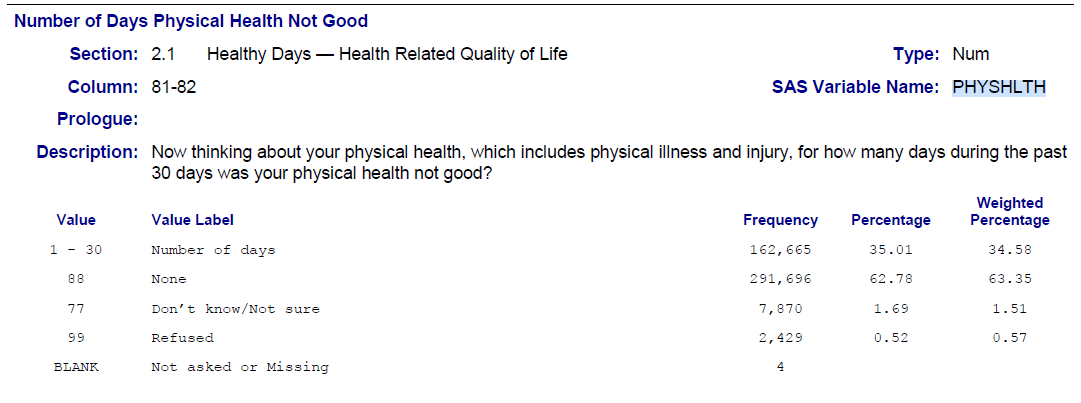
\includegraphics{Pictures/Ch2/CodeBookPHYSHLTH.png}

}

\caption{Evaluate CodeBook Before Making Decisions}

\end{figure}%

\begin{Shaded}
\begin{Highlighting}[]
\NormalTok{brfss }\OtherTok{\textless{}{-}} \FunctionTok{read.csv}\NormalTok{(}\StringTok{"data/brfss.csv"}\NormalTok{)}
\FunctionTok{summary}\NormalTok{(brfss)}
\end{Highlighting}
\end{Shaded}

\begin{verbatim}
    TRNSGNDR        X_AGEG5YR          X_RACE         X_INCOMG    
 Min.   :1.00     Min.   : 1.000   Min.   :1.000   Min.   :1.000  
 1st Qu.:4.00     1st Qu.: 5.000   1st Qu.:1.000   1st Qu.:3.000  
 Median :4.00     Median : 8.000   Median :1.000   Median :5.000  
 Mean   :4.06     Mean   : 7.822   Mean   :1.992   Mean   :4.481  
 3rd Qu.:4.00     3rd Qu.:10.000   3rd Qu.:1.000   3rd Qu.:5.000  
 Max.   :9.00     Max.   :14.000   Max.   :9.000   Max.   :9.000  
 NA's   :310602                    NA's   :94                     
    X_EDUCAG        HLTHPLN1         HADMAM          X_AGE80     
 Min.   :1.000   Min.   :1.000   Min.   :1.00     Min.   :18.00  
 1st Qu.:2.000   1st Qu.:1.000   1st Qu.:1.00     1st Qu.:44.00  
 Median :3.000   Median :1.000   Median :1.00     Median :58.00  
 Mean   :2.966   Mean   :1.108   Mean   :1.22     Mean   :55.49  
 3rd Qu.:4.000   3rd Qu.:1.000   3rd Qu.:1.00     3rd Qu.:69.00  
 Max.   :9.000   Max.   :9.000   Max.   :9.00     Max.   :80.00  
                                 NA's   :208322                  
    PHYSHLTH   
 Min.   : 1.0  
 1st Qu.:20.0  
 Median :88.0  
 Mean   :61.2  
 3rd Qu.:88.0  
 Max.   :99.0  
 NA's   :4     
\end{verbatim}

\subsection{Qualitative Variable}\label{qualitative-variable}

\begin{itemize}
\tightlist
\item
  To look at an example, the one below seeks to understand the
  healthcare issue in reporting gender based on different definitions.
  The dataset is part of the Behavioral Risk Factor Surveillance System
  (brfss) dataset (2014), which includes lots of other variables besides
  reported gender.
\end{itemize}

\begin{Shaded}
\begin{Highlighting}[]
\CommentTok{\# Load the data}
\NormalTok{brfss }\OtherTok{\textless{}{-}} \FunctionTok{read.csv}\NormalTok{(}\StringTok{"data/brfss.csv"}\NormalTok{)}
\CommentTok{\# Summarize the TRNSGNDR variable}
\FunctionTok{summary}\NormalTok{(}\AttributeTok{object =}\NormalTok{ brfss}\SpecialCharTok{$}\NormalTok{TRNSGNDR)}
\end{Highlighting}
\end{Shaded}

\begin{verbatim}
   Min. 1st Qu.  Median    Mean 3rd Qu.    Max.    NA's 
   1.00    4.00    4.00    4.06    4.00    9.00  310602 
\end{verbatim}

\begin{Shaded}
\begin{Highlighting}[]
\CommentTok{\# Find frequencies}
\FunctionTok{table}\NormalTok{(brfss}\SpecialCharTok{$}\NormalTok{TRNSGNDR)}
\end{Highlighting}
\end{Shaded}

\begin{verbatim}

     1      2      3      4      7      9 
   363    212    116 150765   1138   1468 
\end{verbatim}

\begin{itemize}
\tightlist
\item
  Since this table is not very informative, we need to do some edits.
\item
  Check the class of the variable to see the issue with analyzing it as
  a categorical variable.
\end{itemize}

\begin{Shaded}
\begin{Highlighting}[]
\FunctionTok{class}\NormalTok{(brfss}\SpecialCharTok{$}\NormalTok{TRNSGNDR)}
\end{Highlighting}
\end{Shaded}

\begin{verbatim}
[1] "integer"
\end{verbatim}

\begin{itemize}
\tightlist
\item
  First, we need to change the TRNSGNDR variable to a factor using
  as.factor().
\end{itemize}

\begin{Shaded}
\begin{Highlighting}[]
\CommentTok{\# Change variable from numeric to factor}
\NormalTok{brfss}\SpecialCharTok{$}\NormalTok{TRNSGNDR }\OtherTok{\textless{}{-}} \FunctionTok{as.factor}\NormalTok{(brfss}\SpecialCharTok{$}\NormalTok{TRNSGNDR)}
\CommentTok{\# Check data type again to ensure factor}
\FunctionTok{class}\NormalTok{(brfss}\SpecialCharTok{$}\NormalTok{TRNSGNDR)}
\end{Highlighting}
\end{Shaded}

\begin{verbatim}
[1] "factor"
\end{verbatim}

\begin{itemize}
\tightlist
\item
  Then, we need to do some data cleaning on the TRNSGNDR Variable.
\end{itemize}

\begin{Shaded}
\begin{Highlighting}[]
\NormalTok{brfss.cleaned }\OtherTok{\textless{}{-}}\NormalTok{ brfss }\SpecialCharTok{\%\textgreater{}\%} 
  \FunctionTok{mutate}\NormalTok{(}\AttributeTok{TRNSGNDR =} \FunctionTok{recode\_factor}\NormalTok{(TRNSGNDR,}
      \StringTok{\textquotesingle{}1\textquotesingle{}} \OtherTok{=} \StringTok{\textquotesingle{}Male to female\textquotesingle{}}\NormalTok{,}
      \StringTok{\textquotesingle{}2\textquotesingle{}} \OtherTok{=} \StringTok{\textquotesingle{}Female to male\textquotesingle{}}\NormalTok{,}
      \StringTok{\textquotesingle{}3\textquotesingle{}} \OtherTok{=} \StringTok{\textquotesingle{}Gender non{-}conforming\textquotesingle{}}\NormalTok{,}
      \StringTok{\textquotesingle{}4\textquotesingle{}} \OtherTok{=} \StringTok{\textquotesingle{}Not transgender\textquotesingle{}}\NormalTok{,}
      \StringTok{\textquotesingle{}7\textquotesingle{}} \OtherTok{=} \StringTok{\textquotesingle{}Not sure\textquotesingle{}}\NormalTok{,}
      \StringTok{\textquotesingle{}9\textquotesingle{}} \OtherTok{=} \StringTok{\textquotesingle{}Refused\textquotesingle{}}\NormalTok{))}
\end{Highlighting}
\end{Shaded}

\begin{itemize}
\tightlist
\item
  We can use the levels() command to show the factor levels made with
  the mutate() command above.
\end{itemize}

\begin{Shaded}
\begin{Highlighting}[]
\FunctionTok{levels}\NormalTok{(brfss.cleaned}\SpecialCharTok{$}\NormalTok{TRNSGNDR)}
\end{Highlighting}
\end{Shaded}

\begin{verbatim}
[1] "Male to female"        "Female to male"        "Gender non-conforming"
[4] "Not transgender"       "Not sure"              "Refused"              
\end{verbatim}

\begin{itemize}
\tightlist
\item
  Check the summary.
\end{itemize}

\begin{Shaded}
\begin{Highlighting}[]
\FunctionTok{summary}\NormalTok{(brfss.cleaned}\SpecialCharTok{$}\NormalTok{TRNSGNDR)}
\end{Highlighting}
\end{Shaded}

\begin{verbatim}
       Male to female        Female to male Gender non-conforming 
                  363                   212                   116 
      Not transgender              Not sure               Refused 
               150765                  1138                  1468 
                 NA's 
               310602 
\end{verbatim}

\begin{itemize}
\tightlist
\item
  Take a good look at the table to interpret the frequencies in the
  output above. The highest percentage was the ``NA's'' category,
  followed by ``Not transgender''. Removing the NA's moved the ``Not
  transgender'' category to over 97\% of observations.
\end{itemize}

\subsection{Quantitative Variable}\label{quantitative-variable}

\begin{itemize}
\tightlist
\item
  Let's use the cleaned dataset to make more changes to the continuous
  variable PHYSHLTH. In the codebook, it looks like the data is most
  applicable to the first 2 categories. The 1-30 days coding and the 88
  coding, which means 0 days of physical illness and injury.

  \begin{itemize}
  \tightlist
  \item
    Using cleaned data, we need to prep the variable a little more
    before getting an accurate plot.
  \item
    Specifically, we need to null out the 77 and 99 values and make sure
    the 88 coding is set to be 0 for 0 days of illness and injury.
  \end{itemize}
\end{itemize}

\begin{Shaded}
\begin{Highlighting}[]
\NormalTok{brfss.cleaned }\OtherTok{\textless{}{-}}\NormalTok{ brfss }\SpecialCharTok{\%\textgreater{}\%}
    \FunctionTok{mutate}\NormalTok{(}\AttributeTok{TRNSGNDR =} \FunctionTok{recode\_factor}\NormalTok{(TRNSGNDR, }\StringTok{\textasciigrave{}}\AttributeTok{1}\StringTok{\textasciigrave{}} \OtherTok{=} \StringTok{"Male to female"}\NormalTok{, }\StringTok{\textasciigrave{}}\AttributeTok{2}\StringTok{\textasciigrave{}} \OtherTok{=} \StringTok{"Female to male"}\NormalTok{,}
        \StringTok{\textasciigrave{}}\AttributeTok{3}\StringTok{\textasciigrave{}} \OtherTok{=} \StringTok{"Gender non{-}conforming"}\NormalTok{, }\StringTok{\textasciigrave{}}\AttributeTok{4}\StringTok{\textasciigrave{}} \OtherTok{=} \StringTok{"Not transgender"}\NormalTok{, }\StringTok{\textasciigrave{}}\AttributeTok{7}\StringTok{\textasciigrave{}} \OtherTok{=} \StringTok{"Not sure"}\NormalTok{,}
        \StringTok{\textasciigrave{}}\AttributeTok{9}\StringTok{\textasciigrave{}} \OtherTok{=} \StringTok{"Refused"}\NormalTok{)) }\SpecialCharTok{\%\textgreater{}\%}
    \CommentTok{\# Turn the 77 values to NA\textquotesingle{}s.}
\FunctionTok{mutate}\NormalTok{(}\AttributeTok{PHYSHLTH =} \FunctionTok{na\_if}\NormalTok{(PHYSHLTH, }\AttributeTok{y =} \DecValTok{77}\NormalTok{)) }\SpecialCharTok{\%\textgreater{}\%}
    \CommentTok{\# Turn the 99 values to NA\textquotesingle{}s.}
\FunctionTok{mutate}\NormalTok{(}\AttributeTok{PHYSHLTH =} \FunctionTok{na\_if}\NormalTok{(PHYSHLTH, }\AttributeTok{y =} \DecValTok{99}\NormalTok{)) }\SpecialCharTok{\%\textgreater{}\%}
    \CommentTok{\# Recode the 88 values to be numeric value of 0.}
\FunctionTok{mutate}\NormalTok{(}\AttributeTok{PHYSHLTH =} \FunctionTok{recode}\NormalTok{(PHYSHLTH, }\StringTok{\textasciigrave{}}\AttributeTok{88}\StringTok{\textasciigrave{}} \OtherTok{=} \DecValTok{0}\NormalTok{L))}
\end{Highlighting}
\end{Shaded}

\begin{itemize}
\item
  The histogram showed most people have between 0 and 10 unhealthy days
  per 30 days.
\item
  Next, evaluate mean, median, and mode for the PHYSHLTH variable after
  ignoring the blanks.
\end{itemize}

\begin{Shaded}
\begin{Highlighting}[]
\FunctionTok{mean}\NormalTok{(brfss.cleaned}\SpecialCharTok{$}\NormalTok{PHYSHLTH, }\AttributeTok{na.rm =} \ConstantTok{TRUE}\NormalTok{)}
\end{Highlighting}
\end{Shaded}

\begin{verbatim}
[1] 4.224106
\end{verbatim}

\begin{Shaded}
\begin{Highlighting}[]
\FunctionTok{median}\NormalTok{(brfss.cleaned}\SpecialCharTok{$}\NormalTok{PHYSHLTH, }\AttributeTok{na.rm =} \ConstantTok{TRUE}\NormalTok{)}
\end{Highlighting}
\end{Shaded}

\begin{verbatim}
[1] 0
\end{verbatim}

\begin{Shaded}
\begin{Highlighting}[]
\FunctionTok{names}\NormalTok{(}\AttributeTok{x =} \FunctionTok{sort}\NormalTok{(}\AttributeTok{x =} \FunctionTok{table}\NormalTok{(brfss.cleaned}\SpecialCharTok{$}\NormalTok{PHYSHLTH), }\AttributeTok{decreasing =} \ConstantTok{TRUE}\NormalTok{))[}\DecValTok{1}\NormalTok{]}
\end{Highlighting}
\end{Shaded}

\begin{verbatim}
[1] "0"
\end{verbatim}

\begin{itemize}
\tightlist
\item
  While the mean is higher at 4.22, the median and most common number is
  0.
\end{itemize}

\begin{Shaded}
\begin{Highlighting}[]
\DocumentationTok{\#\# Spread to Report with the Mean}
\FunctionTok{var}\NormalTok{(brfss.cleaned}\SpecialCharTok{$}\NormalTok{PHYSHLTH, }\AttributeTok{na.rm =} \ConstantTok{TRUE}\NormalTok{)}
\end{Highlighting}
\end{Shaded}

\begin{verbatim}
[1] 77.00419
\end{verbatim}

\begin{Shaded}
\begin{Highlighting}[]
\FunctionTok{sd}\NormalTok{(brfss.cleaned}\SpecialCharTok{$}\NormalTok{PHYSHLTH, }\AttributeTok{na.rm =} \ConstantTok{TRUE}\NormalTok{)}
\end{Highlighting}
\end{Shaded}

\begin{verbatim}
[1] 8.775203
\end{verbatim}

\begin{Shaded}
\begin{Highlighting}[]
\DocumentationTok{\#\# Spread to Report with Median}
\FunctionTok{summary}\NormalTok{(brfss.cleaned}\SpecialCharTok{$}\NormalTok{PHYSHLTH, }\AttributeTok{na.rm =} \ConstantTok{TRUE}\NormalTok{)}
\end{Highlighting}
\end{Shaded}

\begin{verbatim}
   Min. 1st Qu.  Median    Mean 3rd Qu.    Max.    NA's 
  0.000   0.000   0.000   4.224   3.000  30.000   10303 
\end{verbatim}

\begin{Shaded}
\begin{Highlighting}[]
\FunctionTok{range}\NormalTok{(brfss.cleaned}\SpecialCharTok{$}\NormalTok{PHYSHLTH, }\AttributeTok{na.rm =} \ConstantTok{TRUE}\NormalTok{)}
\end{Highlighting}
\end{Shaded}

\begin{verbatim}
[1]  0 30
\end{verbatim}

\begin{Shaded}
\begin{Highlighting}[]
\FunctionTok{max}\NormalTok{(brfss.cleaned}\SpecialCharTok{$}\NormalTok{PHYSHLTH, }\AttributeTok{na.rm =} \ConstantTok{TRUE}\NormalTok{) }\SpecialCharTok{{-}} \FunctionTok{min}\NormalTok{(brfss.cleaned}\SpecialCharTok{$}\NormalTok{PHYSHLTH,}
    \AttributeTok{na.rm =} \ConstantTok{TRUE}\NormalTok{)}
\end{Highlighting}
\end{Shaded}

\begin{verbatim}
[1] 30
\end{verbatim}

\begin{Shaded}
\begin{Highlighting}[]
\FunctionTok{IQR}\NormalTok{(brfss.cleaned}\SpecialCharTok{$}\NormalTok{PHYSHLTH, }\AttributeTok{na.rm =} \ConstantTok{TRUE}\NormalTok{)}
\end{Highlighting}
\end{Shaded}

\begin{verbatim}
[1] 3
\end{verbatim}

\begin{Shaded}
\begin{Highlighting}[]
\FunctionTok{library}\NormalTok{(semTools)}
\CommentTok{\# Plot the data}
\NormalTok{brfss.cleaned }\SpecialCharTok{\%\textgreater{}\%}
    \FunctionTok{ggplot}\NormalTok{(}\FunctionTok{aes}\NormalTok{(PHYSHLTH)) }\SpecialCharTok{+} \FunctionTok{geom\_histogram}\NormalTok{()}
\end{Highlighting}
\end{Shaded}

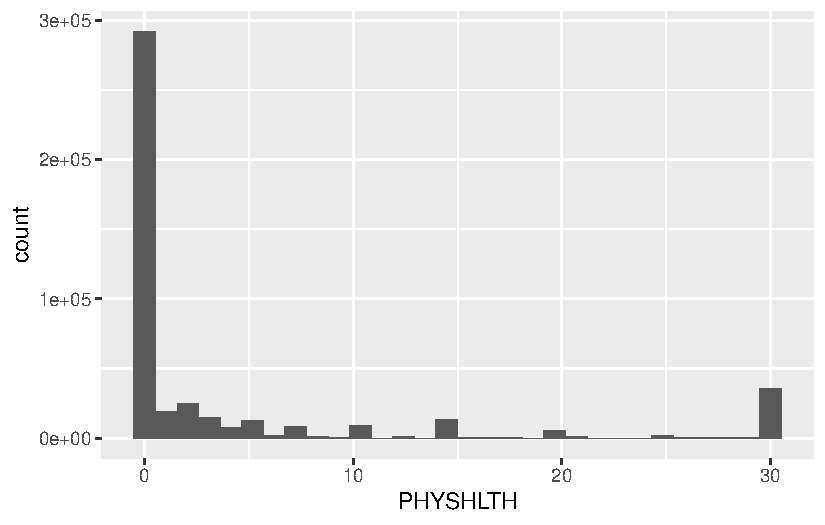
\includegraphics{dataprep_files/figure-pdf/unnamed-chunk-54-1.pdf}

\begin{Shaded}
\begin{Highlighting}[]
\CommentTok{\# Calculate Skewness and Kurtosis}
\FunctionTok{skew}\NormalTok{(brfss.cleaned}\SpecialCharTok{$}\NormalTok{PHYSHLTH)}
\end{Highlighting}
\end{Shaded}

\begin{verbatim}
   skew (g1)           se            z            p 
2.209078e+00 3.633918e-03 6.079054e+02 0.000000e+00 
\end{verbatim}

\begin{Shaded}
\begin{Highlighting}[]
\FunctionTok{kurtosis}\NormalTok{(brfss.cleaned}\SpecialCharTok{$}\NormalTok{PHYSHLTH)}
\end{Highlighting}
\end{Shaded}

\begin{verbatim}
Excess Kur (g2)              se               z               p 
   3.474487e+00    7.267836e-03    4.780634e+02    0.000000e+00 
\end{verbatim}

\begin{itemize}
\tightlist
\item
  The skew results provide a z of 607.905 (6.079054e+02) which is much
  higher than 7 (for large datasets). This indicates a clear right skew
  which means the data is not normally distributed.
\item
  The kurtosis results are also very leptokurtic with a score of
  478.063.
\end{itemize}

\subsection{Using Filters Example}\label{using-filters-example}

\begin{itemize}
\item
  Below takes an example of the brfss data to filter by certain variable
  statuses.

  \begin{itemize}
  \tightlist
  \item
    The first filter() chose observations that were any one of the three
    categories of transgender included in the data. Used the \textbar{}
    ``or'' operator for this filter().
  \item
    The second filter chose people in an age category above category 4
    but below category 12, in the age categories 5 through 11.
  \item
    The last filter used the !is.na to choose observations where HADMAM
    variable was not NA.
  \end{itemize}
\item
  Next, we reduce data set to contain only variables used to create
  table by using the select() command.
\item
  Next, we change all the remaining variables in data set to factors
  using mutate\_all() command. This not only changes the strings to
  factors, but also changes the numerical variables to factors.
\item
  Finally, we use mutate() commands to change the variable category to
  something meaningful(from the codebook).

  \begin{itemize}
  \tightlist
  \item
    Notice the backslash before the apostrophe in Don't in the X\_INCOMG
    recode. This is to prevent the .R file from ending the quotations.
    You could use double quotes around the statement to bypass this, or
    add the backslash like I did here.
  \end{itemize}

\begin{Shaded}
\begin{Highlighting}[]
\NormalTok{brfss\_small }\OtherTok{\textless{}{-}}\NormalTok{ brfss.cleaned }\SpecialCharTok{\%\textgreater{}\%}
    \FunctionTok{filter}\NormalTok{(TRNSGNDR }\SpecialCharTok{==} \StringTok{"Male to female"} \SpecialCharTok{|}\NormalTok{ TRNSGNDR }\SpecialCharTok{==} \StringTok{"Female to male"} \SpecialCharTok{|}
\NormalTok{        TRNSGNDR }\SpecialCharTok{==} \StringTok{"Gender non{-}conforming"}\NormalTok{) }\SpecialCharTok{\%\textgreater{}\%}
    \FunctionTok{filter}\NormalTok{(X\_AGEG5YR }\SpecialCharTok{\textgreater{}} \DecValTok{4} \SpecialCharTok{\&}\NormalTok{ X\_AGEG5YR }\SpecialCharTok{\textless{}} \DecValTok{12}\NormalTok{) }\SpecialCharTok{\%\textgreater{}\%}
    \FunctionTok{filter}\NormalTok{(}\SpecialCharTok{!}\FunctionTok{is.na}\NormalTok{(HADMAM)) }\SpecialCharTok{\%\textgreater{}\%}
    \FunctionTok{select}\NormalTok{(TRNSGNDR, X\_AGEG5YR, X\_RACE, X\_INCOMG, X\_EDUCAG, HLTHPLN1, HADMAM) }\SpecialCharTok{\%\textgreater{}\%}
    \FunctionTok{mutate\_all}\NormalTok{(as.factor) }\SpecialCharTok{\%\textgreater{}\%}
    \CommentTok{\# The next few mutates add labels to categorical variables based}
    \CommentTok{\# on the codebook.}
\FunctionTok{mutate}\NormalTok{(}\AttributeTok{X\_AGEG5YR =} \FunctionTok{recode\_factor}\NormalTok{(X\_AGEG5YR, }\StringTok{\textasciigrave{}}\AttributeTok{5}\StringTok{\textasciigrave{}} \OtherTok{=} \StringTok{"40{-}44"}\NormalTok{, }\StringTok{\textasciigrave{}}\AttributeTok{6}\StringTok{\textasciigrave{}} \OtherTok{=} \StringTok{"45{-}49"}\NormalTok{,}
    \StringTok{\textasciigrave{}}\AttributeTok{7}\StringTok{\textasciigrave{}} \OtherTok{=} \StringTok{"50{-}54"}\NormalTok{, }\StringTok{\textasciigrave{}}\AttributeTok{8}\StringTok{\textasciigrave{}} \OtherTok{=} \StringTok{"55{-}59"}\NormalTok{, }\StringTok{\textasciigrave{}}\AttributeTok{9}\StringTok{\textasciigrave{}} \OtherTok{=} \StringTok{"60{-}64"}\NormalTok{, }\StringTok{\textasciigrave{}}\AttributeTok{10}\StringTok{\textasciigrave{}} \OtherTok{=} \StringTok{"65{-}69"}\NormalTok{, }\StringTok{\textasciigrave{}}\AttributeTok{11}\StringTok{\textasciigrave{}} \OtherTok{=} \StringTok{"70{-}74"}\NormalTok{)) }\SpecialCharTok{\%\textgreater{}\%}
    \FunctionTok{mutate}\NormalTok{(}\AttributeTok{X\_INCOMG =} \FunctionTok{recode\_factor}\NormalTok{(X\_INCOMG, }\StringTok{\textasciigrave{}}\AttributeTok{1}\StringTok{\textasciigrave{}} \OtherTok{=} \StringTok{"Less than 15,000"}\NormalTok{,}
        \StringTok{\textasciigrave{}}\AttributeTok{2}\StringTok{\textasciigrave{}} \OtherTok{=} \StringTok{"15,000 to less than 25,000"}\NormalTok{, }\StringTok{\textasciigrave{}}\AttributeTok{3}\StringTok{\textasciigrave{}} \OtherTok{=} \StringTok{"25,000 to less than 35,000"}\NormalTok{,}
        \StringTok{\textasciigrave{}}\AttributeTok{4}\StringTok{\textasciigrave{}} \OtherTok{=} \StringTok{"35,000 to less than 50,000"}\NormalTok{, }\StringTok{\textasciigrave{}}\AttributeTok{5}\StringTok{\textasciigrave{}} \OtherTok{=} \StringTok{"50,000 or more"}\NormalTok{, }\StringTok{\textasciigrave{}}\AttributeTok{9}\StringTok{\textasciigrave{}} \OtherTok{=} \StringTok{"Don\textquotesingle{}t know/not sure/missing"}\NormalTok{)) }\SpecialCharTok{\%\textgreater{}\%}
    \FunctionTok{mutate}\NormalTok{(}\AttributeTok{X\_EDUCAG =} \FunctionTok{recode\_factor}\NormalTok{(X\_EDUCAG, }\StringTok{\textasciigrave{}}\AttributeTok{1}\StringTok{\textasciigrave{}} \OtherTok{=} \StringTok{"Did not graduate high school"}\NormalTok{,}
        \StringTok{\textasciigrave{}}\AttributeTok{2}\StringTok{\textasciigrave{}} \OtherTok{=} \StringTok{"Graduated high school"}\NormalTok{, }\StringTok{\textasciigrave{}}\AttributeTok{3}\StringTok{\textasciigrave{}} \OtherTok{=} \StringTok{"Attended college/technical school"}\NormalTok{,}
        \StringTok{\textasciigrave{}}\AttributeTok{4}\StringTok{\textasciigrave{}} \OtherTok{=} \StringTok{"Graduated from college/technical school"}\NormalTok{, }\StringTok{\textasciigrave{}}\AttributeTok{9}\StringTok{\textasciigrave{}} \OtherTok{=} \ConstantTok{NA\_character\_}\NormalTok{)) }\SpecialCharTok{\%\textgreater{}\%}
    \FunctionTok{mutate}\NormalTok{(}\AttributeTok{HLTHPLN1 =} \FunctionTok{recode\_factor}\NormalTok{(HLTHPLN1, }\StringTok{\textasciigrave{}}\AttributeTok{1}\StringTok{\textasciigrave{}} \OtherTok{=} \StringTok{"Yes"}\NormalTok{, }\StringTok{\textasciigrave{}}\AttributeTok{2}\StringTok{\textasciigrave{}} \OtherTok{=} \StringTok{"No"}\NormalTok{,}
        \StringTok{\textasciigrave{}}\AttributeTok{7}\StringTok{\textasciigrave{}} \OtherTok{=} \StringTok{"Don\textquotesingle{}t know/not sure/missing"}\NormalTok{, }\StringTok{\textasciigrave{}}\AttributeTok{9}\StringTok{\textasciigrave{}} \OtherTok{=} \StringTok{"Refused"}\NormalTok{)) }\SpecialCharTok{\%\textgreater{}\%}
    \FunctionTok{mutate}\NormalTok{(}\AttributeTok{X\_RACE =} \FunctionTok{recode\_factor}\NormalTok{(X\_RACE, }\StringTok{\textasciigrave{}}\AttributeTok{1}\StringTok{\textasciigrave{}} \OtherTok{=} \StringTok{"White"}\NormalTok{, }\StringTok{\textasciigrave{}}\AttributeTok{2}\StringTok{\textasciigrave{}} \OtherTok{=} \StringTok{"Black"}\NormalTok{,}
        \StringTok{\textasciigrave{}}\AttributeTok{3}\StringTok{\textasciigrave{}} \OtherTok{=} \StringTok{"Native American"}\NormalTok{, }\StringTok{\textasciigrave{}}\AttributeTok{4}\StringTok{\textasciigrave{}} \OtherTok{=} \StringTok{"Asian/Pacific Islander"}\NormalTok{, }\StringTok{\textasciigrave{}}\AttributeTok{5}\StringTok{\textasciigrave{}} \OtherTok{=} \StringTok{"Other"}\NormalTok{,}
        \StringTok{\textasciigrave{}}\AttributeTok{6}\StringTok{\textasciigrave{}} \OtherTok{=} \StringTok{"Other"}\NormalTok{, }\StringTok{\textasciigrave{}}\AttributeTok{7}\StringTok{\textasciigrave{}} \OtherTok{=} \StringTok{"Other"}\NormalTok{, }\StringTok{\textasciigrave{}}\AttributeTok{8}\StringTok{\textasciigrave{}} \OtherTok{=} \StringTok{"Other"}\NormalTok{, }\StringTok{\textasciigrave{}}\AttributeTok{9}\StringTok{\textasciigrave{}} \OtherTok{=} \StringTok{"Other"}\NormalTok{))}
\CommentTok{\# print a summary}
\FunctionTok{summary}\NormalTok{(brfss\_small)}
\end{Highlighting}
\end{Shaded}

\begin{verbatim}
                  TRNSGNDR   X_AGEG5YR                     X_RACE   
 Male to female       : 77   40-44:27   White                 :152  
 Female to male       :113   45-49:27   Black                 : 31  
 Gender non-conforming: 32   50-54:32   Native American       :  4  
 Not transgender      :  0   55-59:44   Asian/Pacific Islander:  6  
 Not sure             :  0   60-64:44   Other                 : 29  
 Refused              :  0   65-69:24                               
                             70-74:24                               
                        X_INCOMG                                     X_EDUCAG 
 Less than 15,000           :46   Did not graduate high school           :24  
 15,000 to less than 25,000 :44   Graduated high school                  :86  
 25,000 to less than 35,000 :19   Attended college/technical school      :68  
 35,000 to less than 50,000 :26   Graduated from college/technical school:44  
 50,000 or more             :65                                               
 Don't know/not sure/missing:22                                               

 HLTHPLN1  HADMAM 
 Yes:198   1:198  
 No : 24   2: 22  
           9:  2  



\end{verbatim}
\item
  This data set full of categorical variables is now fully cleaned and
  ready to be analyzed!
\end{itemize}

\bookmarksetup{startatroot}

\chapter{Summary}\label{summary-3}

\begin{itemize}
\tightlist
\item
  In this lesson, we worked through the basics on data cleaning. Data
  cleaning is so important and there are so many ways to do it. Provided
  are some examples using popular functions in dplyr (under tidyverse).
\end{itemize}

\bookmarksetup{startatroot}

\chapter{Data Visualization}\label{data-visualization}

\begin{itemize}
\tightlist
\item
  The goals this lesson are to be able to create visualizations which
  help to describe a variable or variables more easily (descriptive
  statistics) and to explore patterns in the data based on groups or
  between two or more variables (inferential statistics).
\end{itemize}

\begin{Shaded}
\begin{Highlighting}[]
\DocumentationTok{\#\#\#\#\#\#\#\#\#\#\#\#\#\#\#\#\#\#\#\#\#\#\#\#\#\#\#\#\#\#\#\#\#\#\#\#}
\CommentTok{\# Project name: Data Visualization}
\CommentTok{\# Data used: mtcars {-} part of R. From Blackboard {-} nhanes2012.csv, }
\CommentTok{\# fbi\_deaths.csv., gss.2016.csv, and Edu.csv, UScrime from MASS package}
\CommentTok{\# Libraries used: MASS, tidyverse (ggplot2), semTools}
\DocumentationTok{\#\#\#\#\#\#\#\#\#\#\#\#\#\#\#\#\#\#\#\#\#\#\#\#\#\#\#\#\#\#\#\#\#\#\#\#}
\end{Highlighting}
\end{Shaded}

\section{At a Glance}\label{at-a-glance-2}

\begin{itemize}
\item
  In order to succeed in this lesson, we need to learn how to visualize
  data, noting that there are many ways to do this in R. This lesson
  presents common graphs used in R, and focuses on using ggplot2, a very
  common graphics package that is part of the tidyverse.
\item
  Because packages evolve fairly quickly, parameters within the commands
  shown in this section could evolve and adjust. The best way to figure
  out how to fine-tune your new graph is to explore options and
  parameter settings, while also using the open-source community.
\item
  By the end of this lesson, you should be able to create the following:
\end{itemize}

\begin{enumerate}
\def\labelenumi{\arabic{enumi}.}
\tightlist
\item
  Common Graphs for a Single \emph{Categorical} Variable
\item
  Common Graphs for a Single \emph{Continuous} Variable
\item
  Common Graphs for Two Variables at Once
\end{enumerate}

\begin{itemize}
\tightlist
\item
  This lesson does not provide an exclusive list of what you can do in
  R, but is a good starting point presenting some of the top graphs used
  in statistics with some common parameters added in.
\end{itemize}

\section{Lesson Objectives}\label{lesson-objectives-3}

\begin{itemize}
\tightlist
\item
  Choose and create graphs for a single categorical variable.
\item
  Choose and create graphs for a single continuous variable.
\item
  Choose and create graphs for two variables at once.
\end{itemize}

\bookmarksetup{startatroot}

\chapter{Consider While Reading}\label{consider-while-reading-3}

\begin{itemize}
\item
  It is extremely useful to graph data in R in order to visualize what
  the data is telling us.
\item
  When making graphs, there are a lot of ways to visualize data
  correctly, but there are just as many to do it incorrectly. Be careful
  not to force the data into the story you want it to tell.
\item
  Always be cautious when looking at visuals to make sure the data was
  handled properly.
\item
  The lesson is arranged by first evaluating the variable or variables
  of interest by data type (quantitative or quantitative) and then
  giving some examples of visualizations where this is commonly used. It
  is essential to make sure the variable is in the right data type
  before you create a chart. We look at many charts in this lesson
  including bar charts, density plots, boxplots and scatterplots. A
  multiple boxplot helps us understand the relationship between a
  grouping variable and a numerical variable. The scatterplot helps us
  understand if there is a relationship between two numerical variables
  and it helps us determine whether that relationship is linear or
  nonlinear.
\item
  A lot of graphs you can do in ggplot, you can also do with base R.
  However, ggplot has much more capability to customize a specific
  format for your graphic.

  \begin{itemize}
  \tightlist
  \item
    Base R has many options to graph a variable or variables. If all you
    want is some insight into the data, this might be the way to go.
  \item
    ggplot2 is extremely popular graphing package and has a good pattern
    for making charts. You set the first layer with the ggplot() command
    and then add layers as needed for your graphic.
  \item
    There are also other graphing packages that serve a specific purpose
    (i.e., waffle package in R).
  \end{itemize}
\end{itemize}

\bookmarksetup{startatroot}

\chapter{Graphs for a Single Categorical
Variable}\label{graphs-for-a-single-categorical-variable}

\begin{itemize}
\tightlist
\item
  A categorical variable has categories that are either ordinal with a
  logical order or nominal with no logical order.
\item
  Categorical variables need to be set as the factor data type in R to
  be able to be analyzed and visualized correctly.
\item
  Some common graphing options for single categorical variable:

  \begin{enumerate}
  \def\labelenumi{\arabic{enumi}.}
  \tightlist
  \item
    Bar graph
  \item
    Pie chart
  \end{enumerate}
\item
  In any graph, it is beneficial to do any data cleaning and
  investigation into the variable(s) before you begin. With categorical
  variables, this may require recoding the factor(s) of interest and
  possibly renaming it/them to something meaningful if needed.
\end{itemize}

\section{Bar Graph}\label{bar-graph}

\begin{itemize}
\tightlist
\item
  A bar graph depicts the frequency or the relative frequency for each
  category of the qualitative data as a bar rising vertically from the
  horizontal axis.
\item
  This is also known as a bar chart in which your book refers to as a
  visual display of data often used to examine similarities and
  differences across categories of things; bars can represent
  frequencies, percentages, means, or other statistics.
\item
  We can learn a lot from a bar graph, like the marital status group
  with the highest and lowest frequencies according to the census.gov.
\end{itemize}

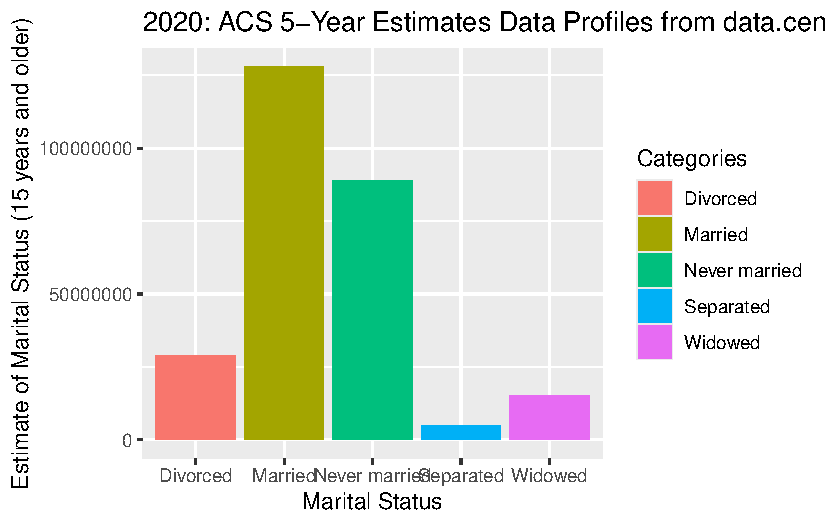
\includegraphics{dataviz_files/figure-pdf/unnamed-chunk-3-1.pdf}

\subsection{geom\_bar()}\label{geom_bar}

\begin{itemize}
\tightlist
\item
  Create a Bar Graph using ggplot() Command
\item
  Like histograms, ggplot has many more parameters available over base R
  to construct bar graphs.
\item
  First, we load tidyerse to access ggplot() command and others. You can
  always do this at the start of all your code to keep all the libraries
  together that are being used.
\end{itemize}

\begin{Shaded}
\begin{Highlighting}[]
\FunctionTok{library}\NormalTok{(}\StringTok{"tidyverse"}\NormalTok{)}
\end{Highlighting}
\end{Shaded}

\begin{itemize}
\tightlist
\item
  ggplot() works in layers, so you will routinely see the \emph{+}
  symbol to kick off a new layer with added functionality.
\item
  Using the ggplot, we always include the aes command first inside the
  ggplot() command. The aes() command is a \emph{quoting function} that
  describes the variables being used. From there, it depends on the
  plot.

  \begin{itemize}
  \tightlist
  \item
    First layer: ggplot() and aes() which calls the dataset and
    variables used.
  \item
    Second layer: Graph type: Bar graph: geom\_bar().
  \item
    Additional layers: labs - for labels including titles; themes; and
    geom\_text. Recreate the example below adding one layer at a time to
    see how the visualization changes.
  \end{itemize}
\end{itemize}

\begin{Shaded}
\begin{Highlighting}[]
\DocumentationTok{\#\# inputting probabilities calculated from a 2023 multiple choice}
\DocumentationTok{\#\# question.  From what you learned about R so far, how do you expect}
\DocumentationTok{\#\# its market share to change?}
\NormalTok{GoUp }\OtherTok{\textless{}{-}} \FloatTok{0.54285}
\NormalTok{GoDown }\OtherTok{\textless{}{-}} \FloatTok{0.03809}
\NormalTok{RemainStable }\OtherTok{\textless{}{-}} \FloatTok{0.34285}
\NormalTok{NoOpinion }\OtherTok{\textless{}{-}} \FloatTok{0.07619}
\CommentTok{\# designing the data frame}
\NormalTok{data\_frame }\OtherTok{\textless{}{-}} \FunctionTok{data.frame}\NormalTok{(}\AttributeTok{Category =} \FunctionTok{c}\NormalTok{(}\StringTok{"Go Up"}\NormalTok{, }\StringTok{"Go Down"}\NormalTok{, }\StringTok{"Remain Stable"}\NormalTok{,}
    \StringTok{"No Opinion"}\NormalTok{), }\AttributeTok{Percentage =} \FunctionTok{c}\NormalTok{(GoUp, GoDown, RemainStable, NoOpinion))}
\CommentTok{\# Making the graph}
\NormalTok{MarketShare }\OtherTok{\textless{}{-}} \FunctionTok{ggplot}\NormalTok{(data\_frame, }\FunctionTok{aes}\NormalTok{(}\AttributeTok{x =}\NormalTok{ Category, }\AttributeTok{y =}\NormalTok{ Percentage, }\AttributeTok{fill =}\NormalTok{ Category)) }\SpecialCharTok{+}
    \FunctionTok{geom\_bar}\NormalTok{(}\AttributeTok{stat =} \StringTok{"identity"}\NormalTok{) }\SpecialCharTok{+} \FunctionTok{labs}\NormalTok{(}\AttributeTok{title =} \StringTok{"How do you expect R\textquotesingle{}s market share to change?"}\NormalTok{,}
    \AttributeTok{x =} \StringTok{"Opinion Category"}\NormalTok{, }\AttributeTok{y =} \StringTok{"Percentage (\%)"}\NormalTok{) }\SpecialCharTok{+} \FunctionTok{theme\_minimal}\NormalTok{() }\SpecialCharTok{+} \FunctionTok{geom\_text}\NormalTok{(}\FunctionTok{aes}\NormalTok{(}\AttributeTok{label =}\NormalTok{ Percentage),}
    \AttributeTok{vjust =} \SpecialCharTok{{-}}\FloatTok{0.5}\NormalTok{, }\AttributeTok{size =} \DecValTok{4}\NormalTok{)}
\NormalTok{MarketShare}
\end{Highlighting}
\end{Shaded}

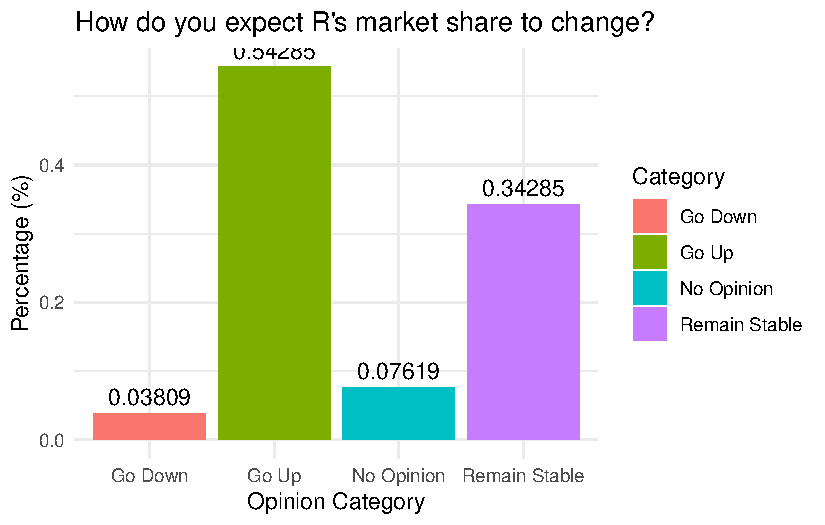
\includegraphics{dataviz_files/figure-pdf/unnamed-chunk-5-1.pdf}

\section{Bar Graph with Data
Wrangling}\label{bar-graph-with-data-wrangling}

\begin{itemize}
\tightlist
\item
  We can also use a dataset to make a bar graph.\\
\item
  Load the Gun related data from the nhanes survey.
\end{itemize}

\begin{Shaded}
\begin{Highlighting}[]
\NormalTok{nhanes }\OtherTok{\textless{}{-}} \FunctionTok{read.csv}\NormalTok{(}\StringTok{"data/nhanes2012.csv"}\NormalTok{)}
\end{Highlighting}
\end{Shaded}

\begin{itemize}
\tightlist
\item
  Next, we need to check the import.
\end{itemize}

\begin{Shaded}
\begin{Highlighting}[]
\CommentTok{\# Results hidden to save space, but gives you the first 6 records in}
\CommentTok{\# the data set.}
\FunctionTok{head}\NormalTok{(nhanes)}
\end{Highlighting}
\end{Shaded}

\begin{itemize}
\tightlist
\item
  We can also check the summary of data of the variable of interest,
  AUQ300, to get a sense of what we are evaluating.
\end{itemize}

\begin{Shaded}
\begin{Highlighting}[]
\FunctionTok{summary}\NormalTok{(nhanes}\SpecialCharTok{$}\NormalTok{AUQ300)}
\end{Highlighting}
\end{Shaded}

\begin{verbatim}
   Min. 1st Qu.  Median    Mean 3rd Qu.    Max.    NA's 
  1.000   1.000   2.000   1.656   2.000   7.000    4689 
\end{verbatim}

\begin{itemize}
\tightlist
\item
  The AUQ300 variable represents gun use. A screenshot of the
  nhanes\_auditory\_2012\_codebook available to you via the book
  resources is copied below so that we can see what AUQ300 really refers
  to. This is always a necessary step because variable names can be
  convoluted and not representative of the variable definition.
\end{itemize}

\begin{figure}[H]

{\centering 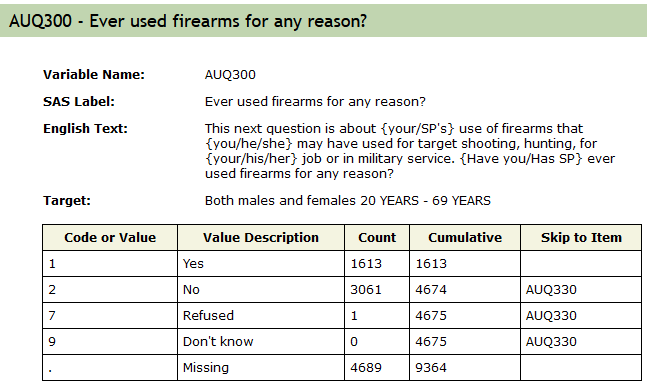
\includegraphics{Pictures/Ch3/AUQ300.png}

}

\caption{AUQ300}

\end{figure}%

\subsubsection{Recode Variable if
Needed}\label{recode-variable-if-needed}

\begin{itemize}
\tightlist
\item
  Look to see if the AUQ300 needs recoding after looking at the codebook
  and making sense of the variable.
\item
  AUQ300 needs to be a factor variable with 1 equaling a \emph{Yes} and
  2 equaling a \emph{No}. We can use recode\_factor to accomplish 2
  things at once with the mutate function.
\item
  recode\_factor() transforms the levels of a categorical variable
  (factor) into a new set of levels and is specific to categorical
  variables.
\item
  recode() is generic and can apply to numerical, categorical, or
  textual data, but still transforms data from one format or code to
  another.
\end{itemize}

\begin{Shaded}
\begin{Highlighting}[]
\NormalTok{nhanes.clean }\OtherTok{\textless{}{-}}\NormalTok{ nhanes }\SpecialCharTok{\%\textgreater{}\%}
    \FunctionTok{mutate}\NormalTok{(}\AttributeTok{AUQ300 =} \FunctionTok{recode\_factor}\NormalTok{(AUQ300, }\StringTok{\textasciigrave{}}\AttributeTok{1}\StringTok{\textasciigrave{}} \OtherTok{=} \StringTok{"Yes"}\NormalTok{, }\StringTok{\textasciigrave{}}\AttributeTok{2}\StringTok{\textasciigrave{}} \OtherTok{=} \StringTok{"No"}\NormalTok{))}
\end{Highlighting}
\end{Shaded}

\begin{itemize}
\tightlist
\item
  Then, we need to check the recode for accuracy. You should see the
  No's and Yes's alongside the rest being coded as NA's.
\end{itemize}

\begin{Shaded}
\begin{Highlighting}[]
\FunctionTok{summary}\NormalTok{(nhanes.clean}\SpecialCharTok{$}\NormalTok{AUQ300)}
\end{Highlighting}
\end{Shaded}

\begin{verbatim}
 Yes   No NA's 
1613 3061 4690 
\end{verbatim}

\subsubsection{Get Bar Roughly Plotted}\label{get-bar-roughly-plotted}

\begin{itemize}
\tightlist
\item
  Start with the basic plot using the ggplot() and geom\_bar() commands.
\item
  Below writes the statement with and without the piping operator.

  \begin{itemize}
  \tightlist
  \item
    Since we are also going to use data preparation techniques, the
    piping operator is recommended.
  \end{itemize}
\end{itemize}

\begin{Shaded}
\begin{Highlighting}[]
\CommentTok{\# Without piping operator}
\FunctionTok{ggplot}\NormalTok{(nhanes.clean, }\FunctionTok{aes}\NormalTok{(}\AttributeTok{x =}\NormalTok{ AUQ300)) }\SpecialCharTok{+} \FunctionTok{geom\_bar}\NormalTok{()}
\end{Highlighting}
\end{Shaded}

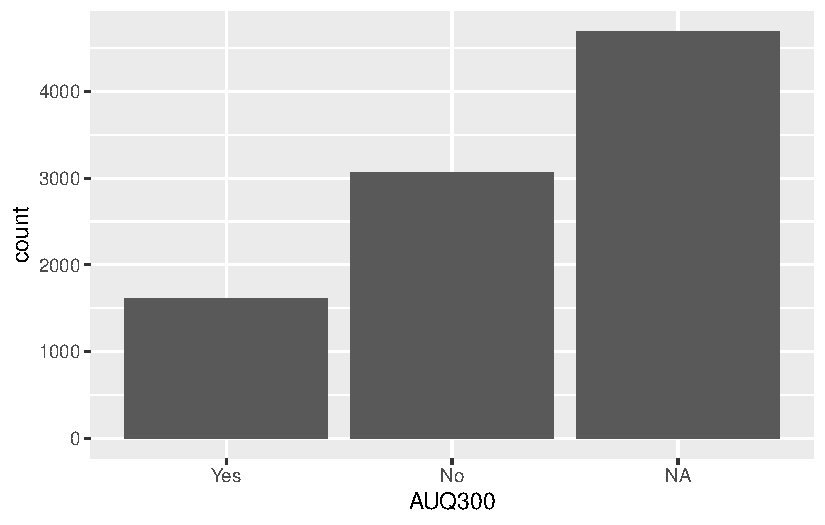
\includegraphics{dataviz_files/figure-pdf/unnamed-chunk-11-1.pdf}

\begin{Shaded}
\begin{Highlighting}[]
\CommentTok{\# With piping operator}
\NormalTok{nhanes.clean }\SpecialCharTok{\%\textgreater{}\%}
    \FunctionTok{ggplot}\NormalTok{(}\FunctionTok{aes}\NormalTok{(}\AttributeTok{x =}\NormalTok{ AUQ300)) }\SpecialCharTok{+} \FunctionTok{geom\_bar}\NormalTok{()}
\end{Highlighting}
\end{Shaded}

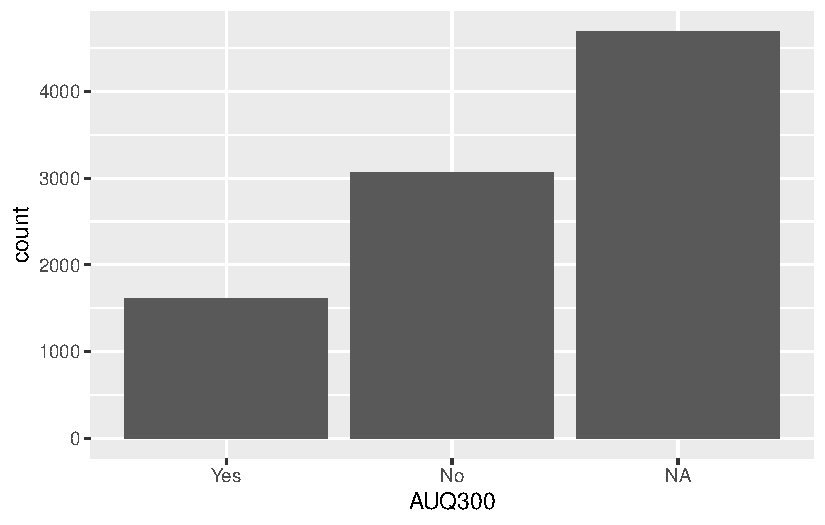
\includegraphics{dataviz_files/figure-pdf/unnamed-chunk-11-2.pdf}

\subsubsection{Add Functions to Clean
Chart}\label{add-functions-to-clean-chart}

\begin{itemize}
\tightlist
\item
  Omit the NA category from AUQ300 variable representing gun use and
  plot it again.
\item
  Add an axis labels under \emph{labs(x = \ldots, y=\ldots)}.
\end{itemize}

\begin{Shaded}
\begin{Highlighting}[]
\NormalTok{nhanes.clean }\SpecialCharTok{\%\textgreater{}\%}
  \FunctionTok{drop\_na}\NormalTok{(AUQ300) }\SpecialCharTok{\%\textgreater{}\%}
  \FunctionTok{ggplot}\NormalTok{(}\FunctionTok{aes}\NormalTok{(}\AttributeTok{x =}\NormalTok{ AUQ300)) }\SpecialCharTok{+} \FunctionTok{geom\_bar}\NormalTok{() }\SpecialCharTok{+}
  \FunctionTok{labs}\NormalTok{(}\AttributeTok{x =} \StringTok{"Gun use"}\NormalTok{, }\AttributeTok{y =} \StringTok{"Number of participants"}\NormalTok{)}
\end{Highlighting}
\end{Shaded}

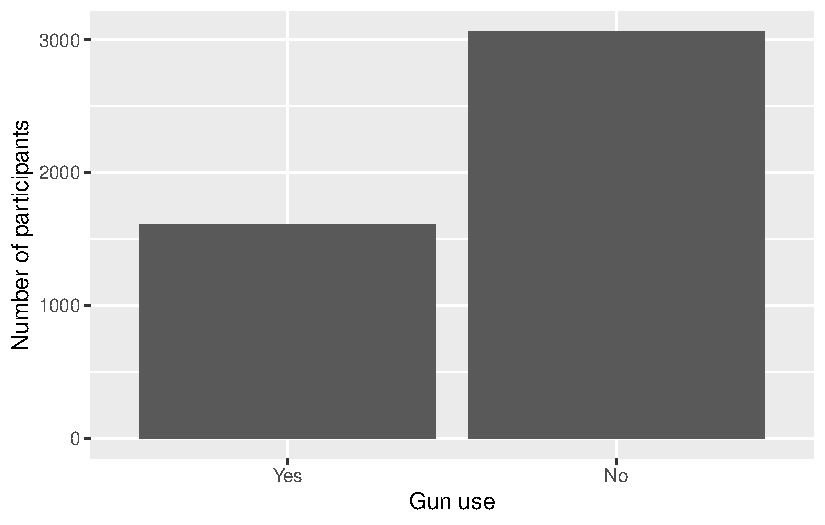
\includegraphics{dataviz_files/figure-pdf/unnamed-chunk-12-1.pdf}

\begin{Shaded}
\begin{Highlighting}[]
\DocumentationTok{\#\#Here, we really benefit from the piping operator because we are doing more than one thing.}
\end{Highlighting}
\end{Shaded}

\begin{itemize}
\tightlist
\item
  From the bar graph, we can see that almost double the amount of people
  have not fired a firearm for any reason than those that fired one.
\end{itemize}

\subsubsection{Adding Color}\label{adding-color}

\begin{itemize}
\item
  There are many ways to add color to a bar graph. Below, the color is
  filled in directly in the aes() command by choosing it to give a
  different color to each categorical value of AUQ300.

  \begin{itemize}
  \tightlist
  \item
    When fill is mapped to a variable, the fill color of the geom will
    vary based on the values of that variable. This is useful for
    distinguishing different groups or categories within the data.
  \end{itemize}
\end{itemize}

\begin{Shaded}
\begin{Highlighting}[]
\NormalTok{nhanes.clean }\SpecialCharTok{\%\textgreater{}\%}
  \FunctionTok{drop\_na}\NormalTok{(AUQ300) }\SpecialCharTok{\%\textgreater{}\%}
  \FunctionTok{ggplot}\NormalTok{(}\FunctionTok{aes}\NormalTok{(AUQ300, }\AttributeTok{fill=}\NormalTok{AUQ300)) }\SpecialCharTok{+}
  \FunctionTok{geom\_bar}\NormalTok{(}\FunctionTok{aes}\NormalTok{(AUQ300)) }\SpecialCharTok{+}
  \FunctionTok{labs}\NormalTok{(}\AttributeTok{x =} \StringTok{"Gun use"}\NormalTok{, }\AttributeTok{y =} \StringTok{"Number of participants"}\NormalTok{, }
       \AttributeTok{subtitle =} \StringTok{"Filled inside the aes()"}\NormalTok{) }
\end{Highlighting}
\end{Shaded}

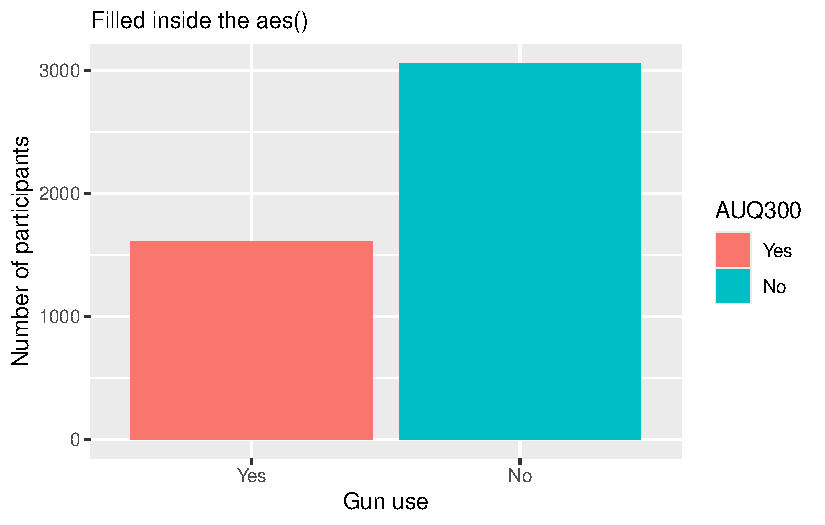
\includegraphics{dataviz_files/figure-pdf/unnamed-chunk-13-1.pdf}

\section{Data Prep and then
Visualized}\label{data-prep-and-then-visualized}

\begin{itemize}
\item
  In the command below, we create a gss.2016.cleaned object to make a
  barplot. In doing so, we do the following:
\item
  Create a bar graph using the ggplot() command, which requires an aes()
  quoting function. This function says that we want to use the grass
  variable in our bar graph.
\item
  Drop all NAs from the grass variable so that legal and not legal are
  the only categories.
\item
  We then create the bars and fill them with 2 colors, red and purple.
  Many color codes can be used here, and will be discussed in a later
  chapter.
\item
  We then add labels to our graph on both x and y axis.
\item
  Finally, we print the new graph, which is saved under the legalize.bar
  object.
\item
  Below, I brought back over the code from the last part in Data
  Preparation. You should still have this in your Chapter1.R file. We
  are going to use that file to create a graphics in R.
\end{itemize}

\begin{Shaded}
\begin{Highlighting}[]
\NormalTok{gss}\FloatTok{.2016} \OtherTok{\textless{}{-}} \FunctionTok{read\_csv}\NormalTok{(}\AttributeTok{file =} \StringTok{"data/gss2016.csv"}\NormalTok{)}
\NormalTok{gss.}\FloatTok{2016.}\NormalTok{cleaned }\OtherTok{\textless{}{-}}\NormalTok{ gss}\FloatTok{.2016} \SpecialCharTok{\%\textgreater{}\%}
    \FunctionTok{mutate}\NormalTok{(}\AttributeTok{grass =} \FunctionTok{as.factor}\NormalTok{(grass)) }\SpecialCharTok{\%\textgreater{}\%}
    \FunctionTok{mutate}\NormalTok{(}\AttributeTok{grass =} \FunctionTok{na\_if}\NormalTok{(}\AttributeTok{x =}\NormalTok{ grass, }\AttributeTok{y =} \StringTok{"DK"}\NormalTok{)) }\SpecialCharTok{\%\textgreater{}\%}
    \FunctionTok{mutate}\NormalTok{(}\AttributeTok{grass =} \FunctionTok{na\_if}\NormalTok{(}\AttributeTok{x =}\NormalTok{ grass, }\AttributeTok{y =} \StringTok{"IAP"}\NormalTok{)) }\SpecialCharTok{\%\textgreater{}\%}
    \FunctionTok{mutate}\NormalTok{(}\AttributeTok{grass =} \FunctionTok{droplevels}\NormalTok{(}\AttributeTok{x =}\NormalTok{ grass)) }\SpecialCharTok{\%\textgreater{}\%}
    \FunctionTok{mutate}\NormalTok{(}\AttributeTok{age =} \FunctionTok{recode}\NormalTok{(age, }\StringTok{\textasciigrave{}}\AttributeTok{89 OR OLDER}\StringTok{\textasciigrave{}} \OtherTok{=} \StringTok{"89"}\NormalTok{)) }\SpecialCharTok{\%\textgreater{}\%}
    \FunctionTok{mutate}\NormalTok{(}\AttributeTok{age =} \FunctionTok{as.numeric}\NormalTok{(}\AttributeTok{x =}\NormalTok{ age)) }\SpecialCharTok{\%\textgreater{}\%}
    \FunctionTok{mutate}\NormalTok{(}\AttributeTok{age.cat =} \FunctionTok{cut}\NormalTok{(}\AttributeTok{x =}\NormalTok{ age, }\AttributeTok{breaks =} \FunctionTok{c}\NormalTok{(}\SpecialCharTok{{-}}\ConstantTok{Inf}\NormalTok{, }\DecValTok{29}\NormalTok{, }\DecValTok{59}\NormalTok{, }\DecValTok{74}\NormalTok{, }\ConstantTok{Inf}\NormalTok{), }\AttributeTok{labels =} \FunctionTok{c}\NormalTok{(}\StringTok{"\textless{} 30"}\NormalTok{,}
        \StringTok{"30 {-} 59"}\NormalTok{, }\StringTok{"60 {-} 74"}\NormalTok{, }\StringTok{"75+"}\NormalTok{)))}
\end{Highlighting}
\end{Shaded}

\begin{itemize}
\tightlist
\item
  Once the data is prepped, we can graph the variable or variables.
\end{itemize}

\begin{Shaded}
\begin{Highlighting}[]
\CommentTok{\# Make a Bar Graph for Grass Variable}
\NormalTok{legalize.bar }\OtherTok{\textless{}{-}}\NormalTok{ gss.}\FloatTok{2016.}\NormalTok{cleaned }\SpecialCharTok{\%\textgreater{}\%}
    \FunctionTok{drop\_na}\NormalTok{(grass) }\SpecialCharTok{\%\textgreater{}\%}
    \FunctionTok{ggplot}\NormalTok{(}\FunctionTok{aes}\NormalTok{(}\AttributeTok{x =}\NormalTok{ grass)) }\SpecialCharTok{+} \FunctionTok{geom\_bar}\NormalTok{(}\AttributeTok{fill =} \FunctionTok{c}\NormalTok{(}\StringTok{"red"}\NormalTok{, }\StringTok{"purple"}\NormalTok{)) }\SpecialCharTok{+} \FunctionTok{labs}\NormalTok{(}\AttributeTok{x =} \StringTok{"Should marijuana be legal?"}\NormalTok{,}
    \AttributeTok{y =} \StringTok{"Percent of responses"}\NormalTok{)}
\NormalTok{legalize.bar}
\end{Highlighting}
\end{Shaded}

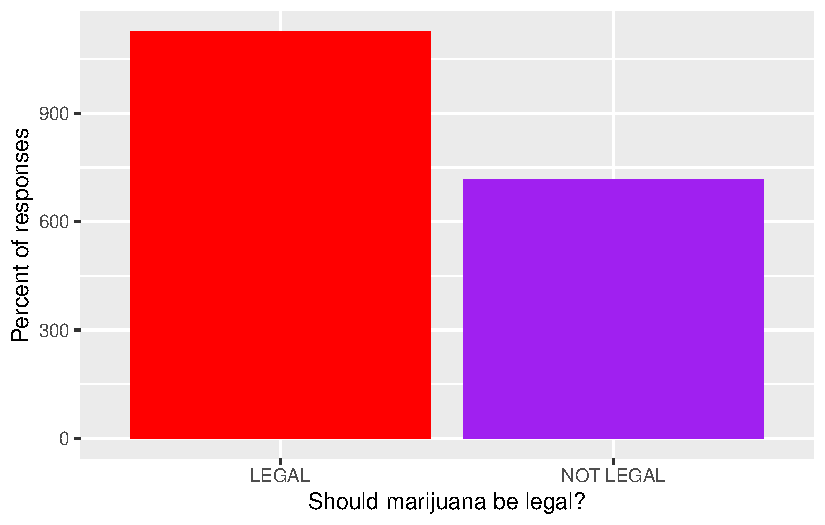
\includegraphics{dataviz_files/figure-pdf/unnamed-chunk-15-1.pdf}

\section{Edit The Graphic}\label{edit-the-graphic}

\begin{itemize}
\tightlist
\item
  Next, we can edit these commands to include the age variable. The
  aes() quoting function has expanded to have the bars filled color
  using the grass variable, the age category has replaced the grass
  variable on the x axis, and there is a new a formula on the y axis to
  sum and count.
\item
  We also gave this a theme and updated the labels.
\end{itemize}

\begin{Shaded}
\begin{Highlighting}[]
\NormalTok{legalize.bar }\OtherTok{\textless{}{-}}\NormalTok{ gss.}\FloatTok{2016.}\NormalTok{cleaned }\SpecialCharTok{\%\textgreater{}\%}
    \FunctionTok{drop\_na}\NormalTok{() }\SpecialCharTok{\%\textgreater{}\%}
    \FunctionTok{ggplot}\NormalTok{(}\FunctionTok{aes}\NormalTok{(age.cat, }\AttributeTok{y =} \DecValTok{100} \SpecialCharTok{*}\NormalTok{ (}\FunctionTok{after\_stat}\NormalTok{(count))}\SpecialCharTok{/}\FunctionTok{sum}\NormalTok{(}\FunctionTok{after\_stat}\NormalTok{(count)),}
        \AttributeTok{fill =}\NormalTok{ grass)) }\SpecialCharTok{+} \FunctionTok{geom\_bar}\NormalTok{(}\AttributeTok{position =} \StringTok{"dodge"}\NormalTok{) }\SpecialCharTok{+} \FunctionTok{theme\_minimal}\NormalTok{() }\SpecialCharTok{+}
    \FunctionTok{labs}\NormalTok{(}\AttributeTok{x =} \StringTok{"Age Category"}\NormalTok{, }\AttributeTok{y =} \StringTok{"Percent of responses"}\NormalTok{)}

\NormalTok{legalize.bar}
\end{Highlighting}
\end{Shaded}

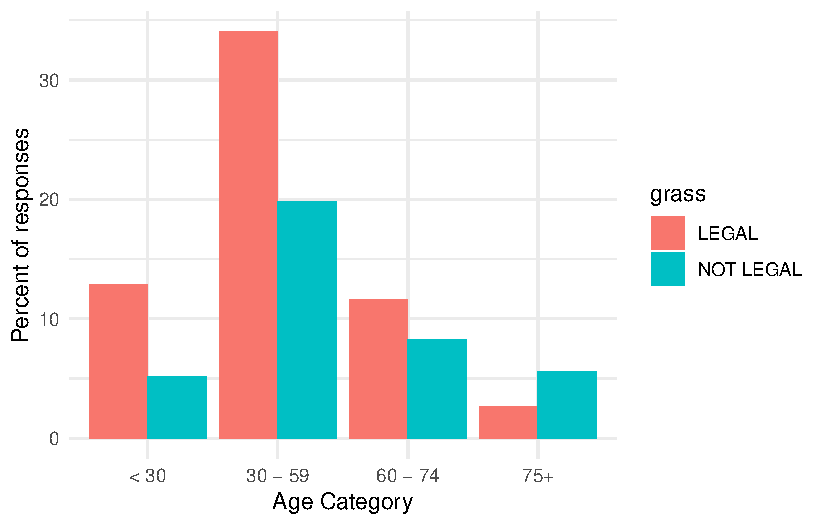
\includegraphics{dataviz_files/figure-pdf/unnamed-chunk-16-1.pdf}

\begin{itemize}
\tightlist
\item
  Evaluate these 2 graphs and see what information you can get from
  them.
\end{itemize}

\section{Pie Chart}\label{pie-chart}

\begin{itemize}
\tightlist
\item
  A pie chart is a segmented circle whose segments portray the relative
  frequencies of the categories of a qualitative variable.
\item
  Slices of pie in different colors represent the parts.
\item
  In this example, the firearm is divided by type to show parts of a
  whole, where the total of the proportions must add to 1.0 and the
  total of the percentages must add to 100\%.
\end{itemize}

\begin{Shaded}
\begin{Highlighting}[]
\CommentTok{\# Importing data from working directory}
\NormalTok{fbi.deaths }\OtherTok{\textless{}{-}} \FunctionTok{read.csv}\NormalTok{(}\StringTok{"data/fbi\_deaths.csv"}\NormalTok{, }\AttributeTok{stringsAsFactors =} \ConstantTok{TRUE}\NormalTok{)}
\CommentTok{\# Selecting rows of interest for pie chart}
\NormalTok{fbi.deaths.small }\OtherTok{\textless{}{-}}\NormalTok{ fbi.deaths[}\FunctionTok{c}\NormalTok{(}\DecValTok{3}\NormalTok{, }\DecValTok{4}\NormalTok{, }\DecValTok{5}\NormalTok{, }\DecValTok{6}\NormalTok{, }\DecValTok{7}\NormalTok{), ]}
\NormalTok{fbi.deaths.small }\OtherTok{\textless{}{-}}\NormalTok{ fbi.deaths.small }\SpecialCharTok{\%\textgreater{}\%}
    \FunctionTok{rename}\NormalTok{(}\AttributeTok{Weapon =}\NormalTok{ X)}
\CommentTok{\# Checking summary of fbi deaths}
\FunctionTok{summary}\NormalTok{(fbi.deaths.small)}
\end{Highlighting}
\end{Shaded}

\begin{verbatim}
                       Weapon      X2012          X2013          X2014     
 Firearms, type not stated:1   Min.   : 116   Min.   : 123   Min.   :  93  
 Handguns                 :1   1st Qu.: 298   1st Qu.: 285   1st Qu.: 258  
 Other guns               :1   Median : 310   Median : 308   Median : 264  
 Rifles                   :1   Mean   :1779   Mean   :1691   Mean   :1662  
 Shotguns                 :1   3rd Qu.:1769   3rd Qu.:1956   3rd Qu.:2024  
 Asphyxiation             :0   Max.   :6404   Max.   :5782   Max.   :5673  
 (Other)                  :0                                               
     X2015          X2016     
 Min.   : 177   Min.   : 186  
 1st Qu.: 258   1st Qu.: 262  
 Median : 272   Median : 374  
 Mean   :1956   Mean   :2201  
 3rd Qu.:2502   3rd Qu.:3077  
 Max.   :6569   Max.   :7105  
                              
\end{verbatim}

\begin{itemize}
\tightlist
\item
  Again, ggplot works in layers, so in order to make a pie, you need a
  few layers and have a few optional ones.

  \begin{itemize}
  \tightlist
  \item
    The aes() command specifies the variable to create the pie, in this
    case x2016.
  \item
    geom\_col() sets the borders of the pie and makes it visible.
  \item
    coord\_polar() command makes the pie circular.
  \item
    theme\_void() command is optional and adjusts the theme of the pie.
    to remove axis, background, etc.
  \end{itemize}
\end{itemize}

\begin{Shaded}
\begin{Highlighting}[]
\FunctionTok{ggplot}\NormalTok{(fbi.deaths.small, }\FunctionTok{aes}\NormalTok{(}\AttributeTok{x=}\StringTok{""}\NormalTok{, }\AttributeTok{y=}\NormalTok{X2016, }\AttributeTok{fill=}\NormalTok{Weapon)) }\SpecialCharTok{+}
  \FunctionTok{geom\_col}\NormalTok{() }\SpecialCharTok{+} 
  \FunctionTok{coord\_polar}\NormalTok{(}\StringTok{"y"}\NormalTok{, }\AttributeTok{start=}\DecValTok{0}\NormalTok{) }\SpecialCharTok{+} 
  \FunctionTok{theme\_void}\NormalTok{() }
\end{Highlighting}
\end{Shaded}

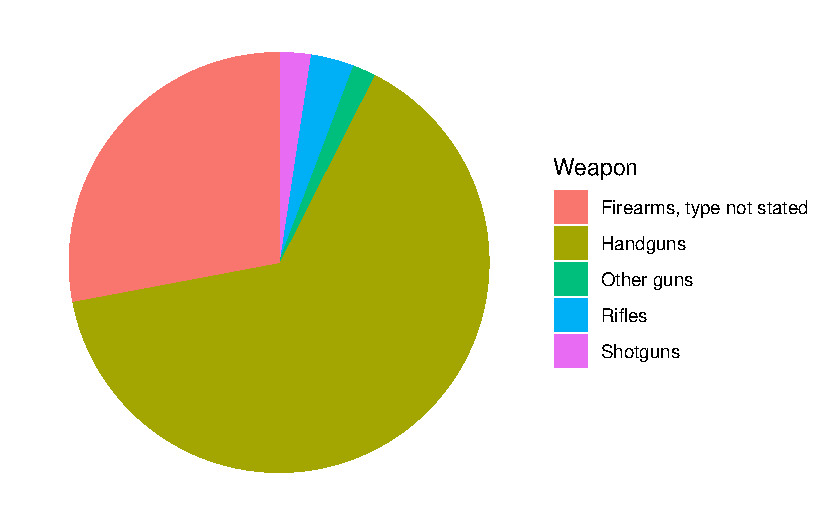
\includegraphics{dataviz_files/figure-pdf/unnamed-chunk-18-1.pdf}

\begin{itemize}
\tightlist
\item
  From the pie, we can see that the majority of weapons that caused fbi
  gun related deaths are handguns followed by a type of firearm that is
  not stated.
\end{itemize}

\section{Comparison of Charts}\label{comparison-of-charts}

\begin{itemize}
\tightlist
\item
  Recommended graphs for single categorical or factor type variable:

  \begin{itemize}
  \tightlist
  \item
    Bar graph, for showing relative group sizes.
  \item
    Pie charts are available in R but are not recommended because they
    tend to be less clear for comparing group sizes.

    \begin{itemize}
    \tightlist
    \item
      Pie charts are difficult to read since the relative size of pie
      pieces is often hard to determine.
    \item
      Pie charts take up a lot of space to convey little information.
    \item
      People often use fancy formatting like 3D, which takes up more
      space and makes understanding relative size of pie pieces even
      more difficult.
    \end{itemize}
  \end{itemize}
\end{itemize}

\bookmarksetup{startatroot}

\chapter{Graphs for a Single Continuous
Variable}\label{graphs-for-a-single-continuous-variable}

\begin{itemize}
\tightlist
\item
  A continuous variable refers to a variable that can take any value
  over a range of values.
\item
  A continuous variable needs to be numeric, and could be integer type
  or numeric type in R. Just like with graphs that include categorical
  variables, it is beneficial to do any data cleaning and investigation
  into the variable(s) before you begin. With continuous variables, this
  may require recoding the variable to coerce it to the appropriate data
  type and/or renaming it to something meaningful if needed.
\item
  It is also beneficial to make sure the numerical variable is indeed
  supposed to be numerical (as opposed to a factor). For instance, you
  commonly see numbers listed for categories like the Yes/No coded as a
  1/2, such as with the AUQ300 variable.
\end{itemize}

Some common graphing options for single continuous variable:

\begin{itemize}
\tightlist
\item
  Histograms (From Lesson 2)
\item
  Density plots
\item
  Boxplots
\end{itemize}

\section{Histograms}\label{histograms-1}

\begin{itemize}
\item
  A histogram is a useful plot to determine central tendency and spread.
\item
  We went over histograms in Lesson 2, so refer back for information on
  how to create a histogram using base R and ggplot.
\item
  Remember that you can tell the distribution from a histogram, and that
  distribution can be normal or skewed (Right or Left).\\
\item
  With each chart based on quantitative data, you should be able to get
  a sense of the distribution.
\item
  The histogram below looks right skewed.
\end{itemize}

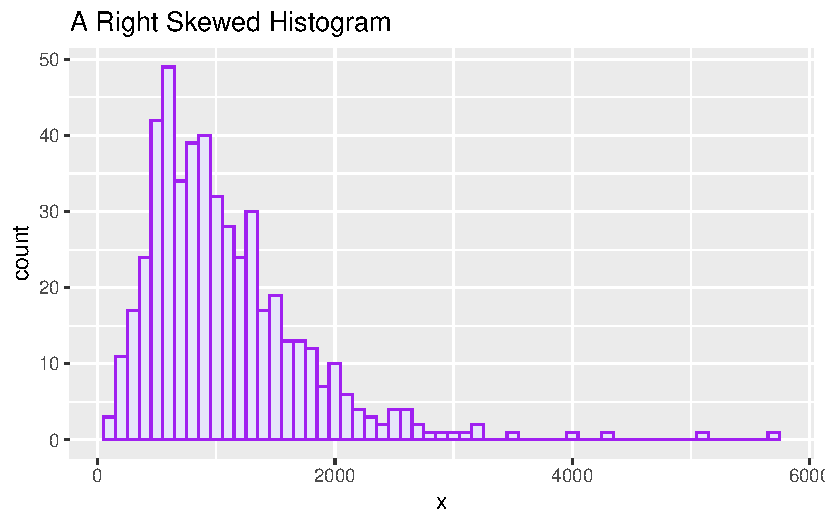
\includegraphics{dataviz_files/figure-pdf/unnamed-chunk-19-1.pdf}

\section{Density Plots}\label{density-plots}

\begin{itemize}
\item
  A density plot is similar to a histogram but more fluid in appearance
  because it does not have the separate bins.\\
\item
  \emph{Probability density} is not very useful for interpreting what is
  happening at any given value of the variable on the x-axis, but it is
  useful in computing the percentage of values that are within a range
  along the x-axis.
\item
  The \emph{area under the curve} in a density plot could be interpreted
  as the probability of a single observation or a range of observations.
\item
  We can use random normal data to create the density plot like shown
  below with a sample of 1000, a mean of 10 and a standard deviation of
  2. To do this, we need to make the vector and assign it to a data
  frame.
\item
  In R, set.seed() is a function used to set the seed for random number
  generation. By setting a seed using set.seed(), you ensure
  reproducibility of your code. If you run the same code with the same
  seed, you'll get the same sequence of random numbers every time. This
  is particularly useful for debugging, testing, or when you want to
  ensure that your results are reproducible.
\item
  We use set.seed before any function with a random normal generator to
  ensure reproducibility.
\item
  If a dataset is provided, then you do not need to generate your own
  random data as shown in the step below.
\end{itemize}

\begin{Shaded}
\begin{Highlighting}[]
\FunctionTok{set.seed}\NormalTok{(}\DecValTok{1}\NormalTok{)}
\NormalTok{x }\OtherTok{\textless{}{-}} \FunctionTok{rnorm}\NormalTok{(}\DecValTok{1000}\NormalTok{, }\AttributeTok{mean =} \DecValTok{10}\NormalTok{, }\AttributeTok{sd =} \DecValTok{2}\NormalTok{)}
\NormalTok{df }\OtherTok{\textless{}{-}} \FunctionTok{data.frame}\NormalTok{(x)}
\end{Highlighting}
\end{Shaded}

\begin{itemize}
\tightlist
\item
  Next, we can make the density plot using the ggplot2 package under
  tidyverse.

  \begin{itemize}
  \tightlist
  \item
    Layer 2 includes the geom\_density() command in addition to the
    standard Layer 1 ggplot() command to create the density plot.
  \end{itemize}
\end{itemize}

\begin{Shaded}
\begin{Highlighting}[]
\FunctionTok{ggplot}\NormalTok{(df, }\FunctionTok{aes}\NormalTok{(x)) }\SpecialCharTok{+} \FunctionTok{geom\_density}\NormalTok{()}
\end{Highlighting}
\end{Shaded}

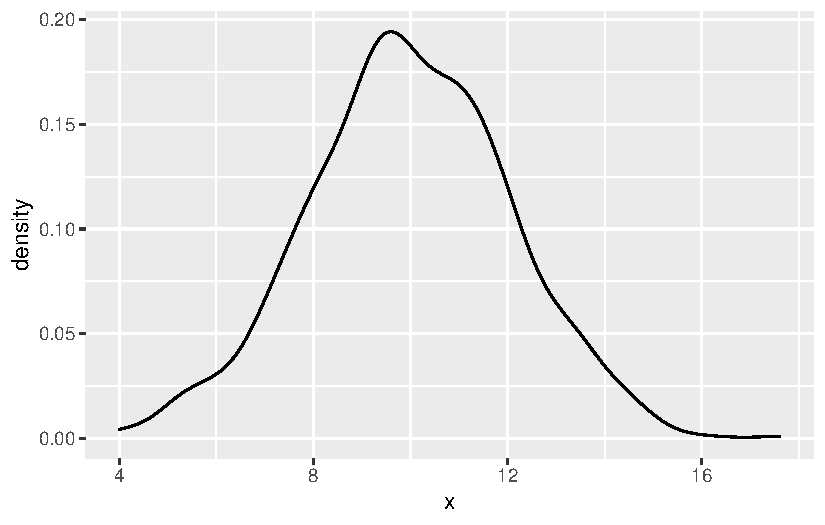
\includegraphics{dataviz_files/figure-pdf/unnamed-chunk-21-1.pdf}

\begin{itemize}
\tightlist
\item
  There are a lot of arguments you can change. I selected a couple
  below. Be sure to look at the help file on the geom\_density() layer
  to get the variety on what you can do.

  \begin{itemize}
  \tightlist
  \item
    color = sets a line color
  \item
    lwd = makes the line thicker. Increase this number for thicker line.
  \item
    fill= colors the area under the curve.
  \item
    alpha= sets the transparency to the area under the curve.
  \end{itemize}
\end{itemize}

\begin{Shaded}
\begin{Highlighting}[]
\FunctionTok{ggplot}\NormalTok{(df, }\FunctionTok{aes}\NormalTok{(x)) }\SpecialCharTok{+} \FunctionTok{geom\_density}\NormalTok{(}\AttributeTok{color =} \StringTok{"darkblue"}\NormalTok{, }\AttributeTok{lwd =} \DecValTok{3}\NormalTok{)}
\end{Highlighting}
\end{Shaded}

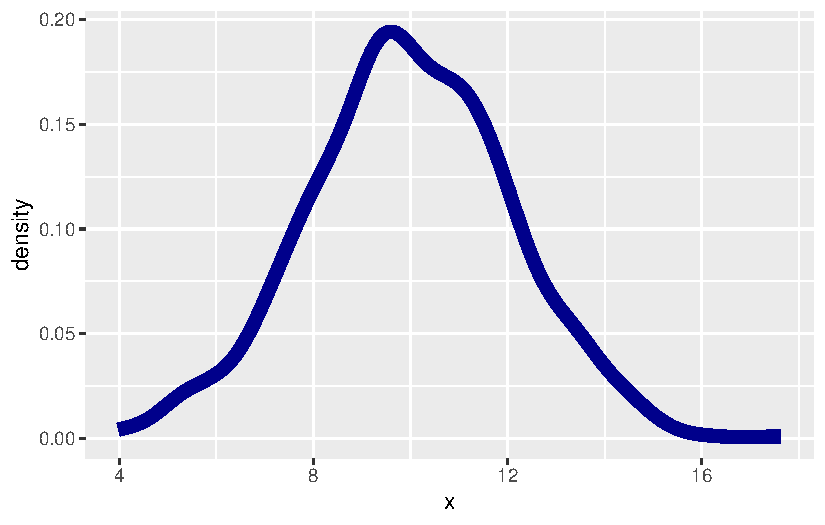
\includegraphics{dataviz_files/figure-pdf/unnamed-chunk-22-1.pdf}

\begin{Shaded}
\begin{Highlighting}[]
\FunctionTok{ggplot}\NormalTok{(df, }\FunctionTok{aes}\NormalTok{(x)) }\SpecialCharTok{+}
  \FunctionTok{geom\_density}\NormalTok{(}\AttributeTok{color =} \StringTok{"darkblue"}\NormalTok{, }
    \CommentTok{\#fill = Fills color under the curve}
    \AttributeTok{fill =} \StringTok{"lightblue"}\NormalTok{,}
    \CommentTok{\#alpha = Sets a transparency to the area under the curve. }
    \CommentTok{\#.5 for 50\% transparency. }
    \AttributeTok{alpha =}\NormalTok{ .}\DecValTok{5}\NormalTok{) }
\end{Highlighting}
\end{Shaded}

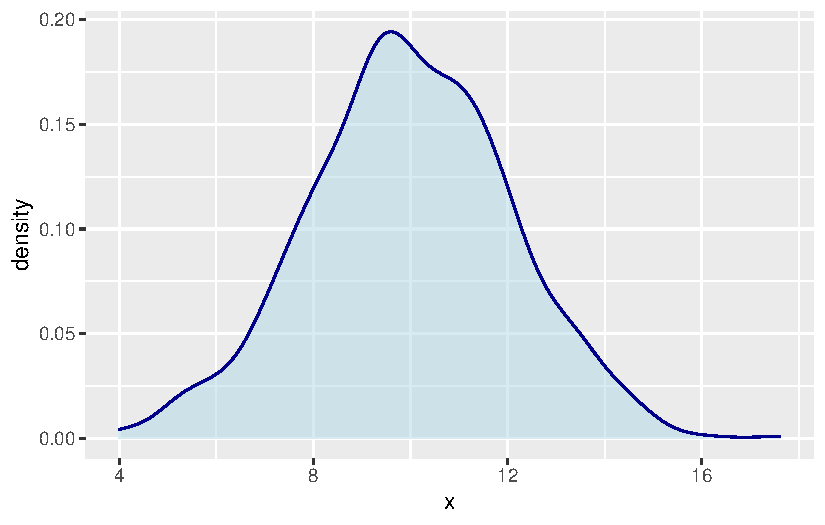
\includegraphics{dataviz_files/figure-pdf/unnamed-chunk-23-1.pdf}

\begin{itemize}
\tightlist
\item
  We can even add a mean line, which we know in this case is 10 because
  we used random normal data with that mean set as a parameter.
\item
  geom\_vline() is a function used to add vertical lines to a plot
  created with ggplot. This function is useful for visually indicating
  specific points or ranges on the x-axis.
\item
  You can do a line break in your R code after a comma (\(,\)) or after
  a plus sign (\(+\)). I find things easier to read on less lines, but
  it is personal preference how many lines you use given still following
  the rules in R.
\end{itemize}

\begin{Shaded}
\begin{Highlighting}[]
\FunctionTok{ggplot}\NormalTok{(df, }\FunctionTok{aes}\NormalTok{(x)) }\SpecialCharTok{+} \FunctionTok{geom\_density}\NormalTok{(}\AttributeTok{color =} \StringTok{"darkblue"}\NormalTok{, }\AttributeTok{fill =} \StringTok{"lightblue"}\NormalTok{,}
    \AttributeTok{alpha =} \FloatTok{0.5}\NormalTok{) }\SpecialCharTok{+} \FunctionTok{geom\_vline}\NormalTok{(}\FunctionTok{aes}\NormalTok{(}\AttributeTok{xintercept =} \FunctionTok{mean}\NormalTok{(x)), }\AttributeTok{color =} \StringTok{"red"}\NormalTok{,}
    \AttributeTok{linetype =} \StringTok{"dashed"}\NormalTok{, }\AttributeTok{lwd =} \DecValTok{1}\NormalTok{)}
\end{Highlighting}
\end{Shaded}

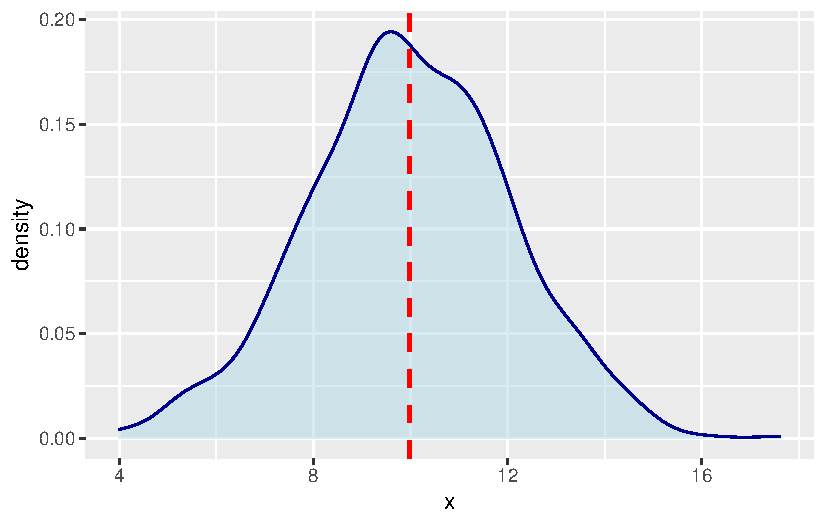
\includegraphics{dataviz_files/figure-pdf/unnamed-chunk-24-1.pdf}

\section{Boxplot}\label{boxplot}

\begin{itemize}
\item
  A boxplot is a visual representation of data that shows central
  tendency (usually the median) and spread (usually the interquartile
  range) of a numeric variable for one or more groups.
\item
  Boxplots are often used to compare the distribution of a continuous
  variable across several groups.
\item
  A box plot allows you to:

  \begin{itemize}
  \tightlist
  \item
    Graphically display the distribution of a data set.
  \item
    Compare two or more distributions.
  \item
    Identify outliers in a data set.
  \end{itemize}
\end{itemize}

\begin{figure}[H]

{\centering 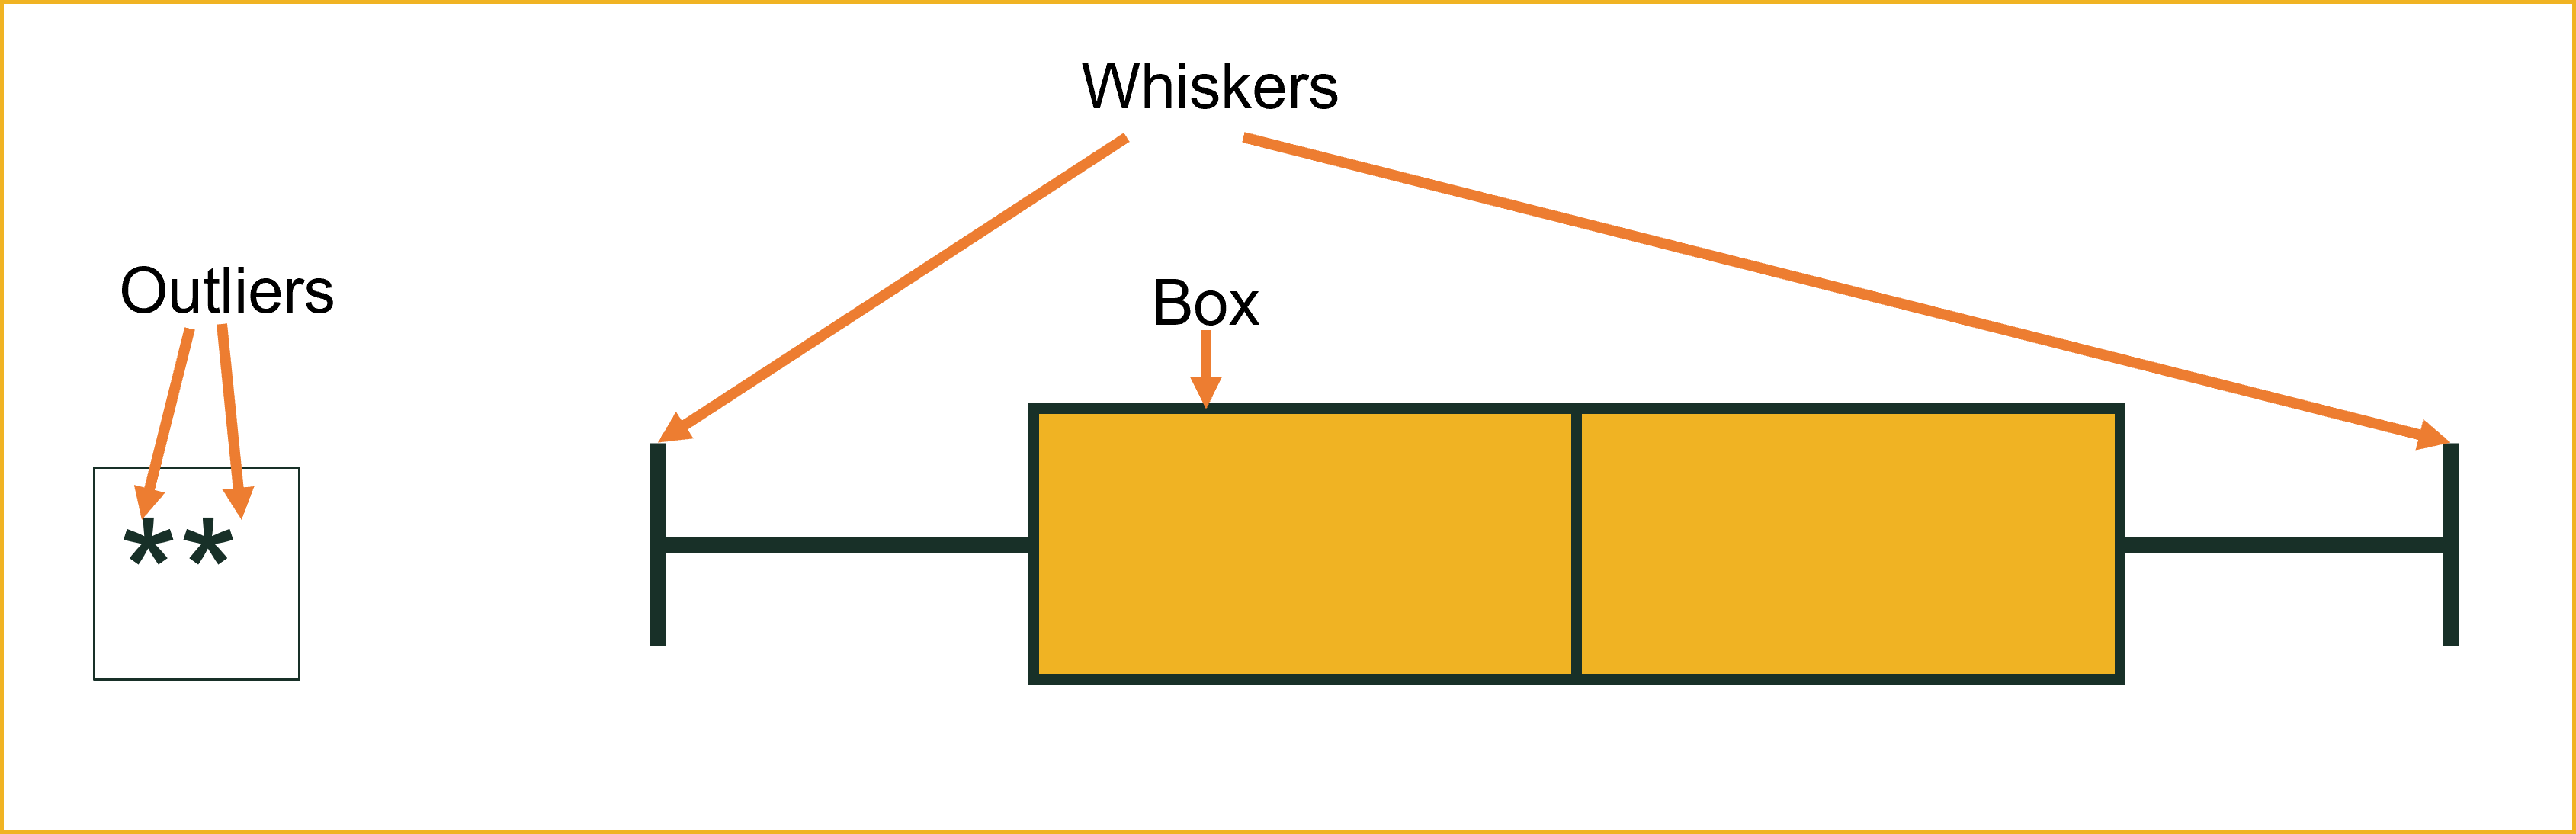
\includegraphics{Pictures/Ch3/Boxplot.png}

}

\caption{A Boxplot with Outliers on Left}

\end{figure}%

\begin{itemize}
\tightlist
\item
  Boxplots include the following information:

  \begin{itemize}
  \tightlist
  \item
    A line representing the median value.
  \item
    A box containing the middle 50\% of values.
  \item
    Whiskers extending to 1.5 times the IQR.
  \item
    Outliers more than 1.5 times the IQR away from the median.
  \end{itemize}
\end{itemize}

\begin{figure}[H]

{\centering 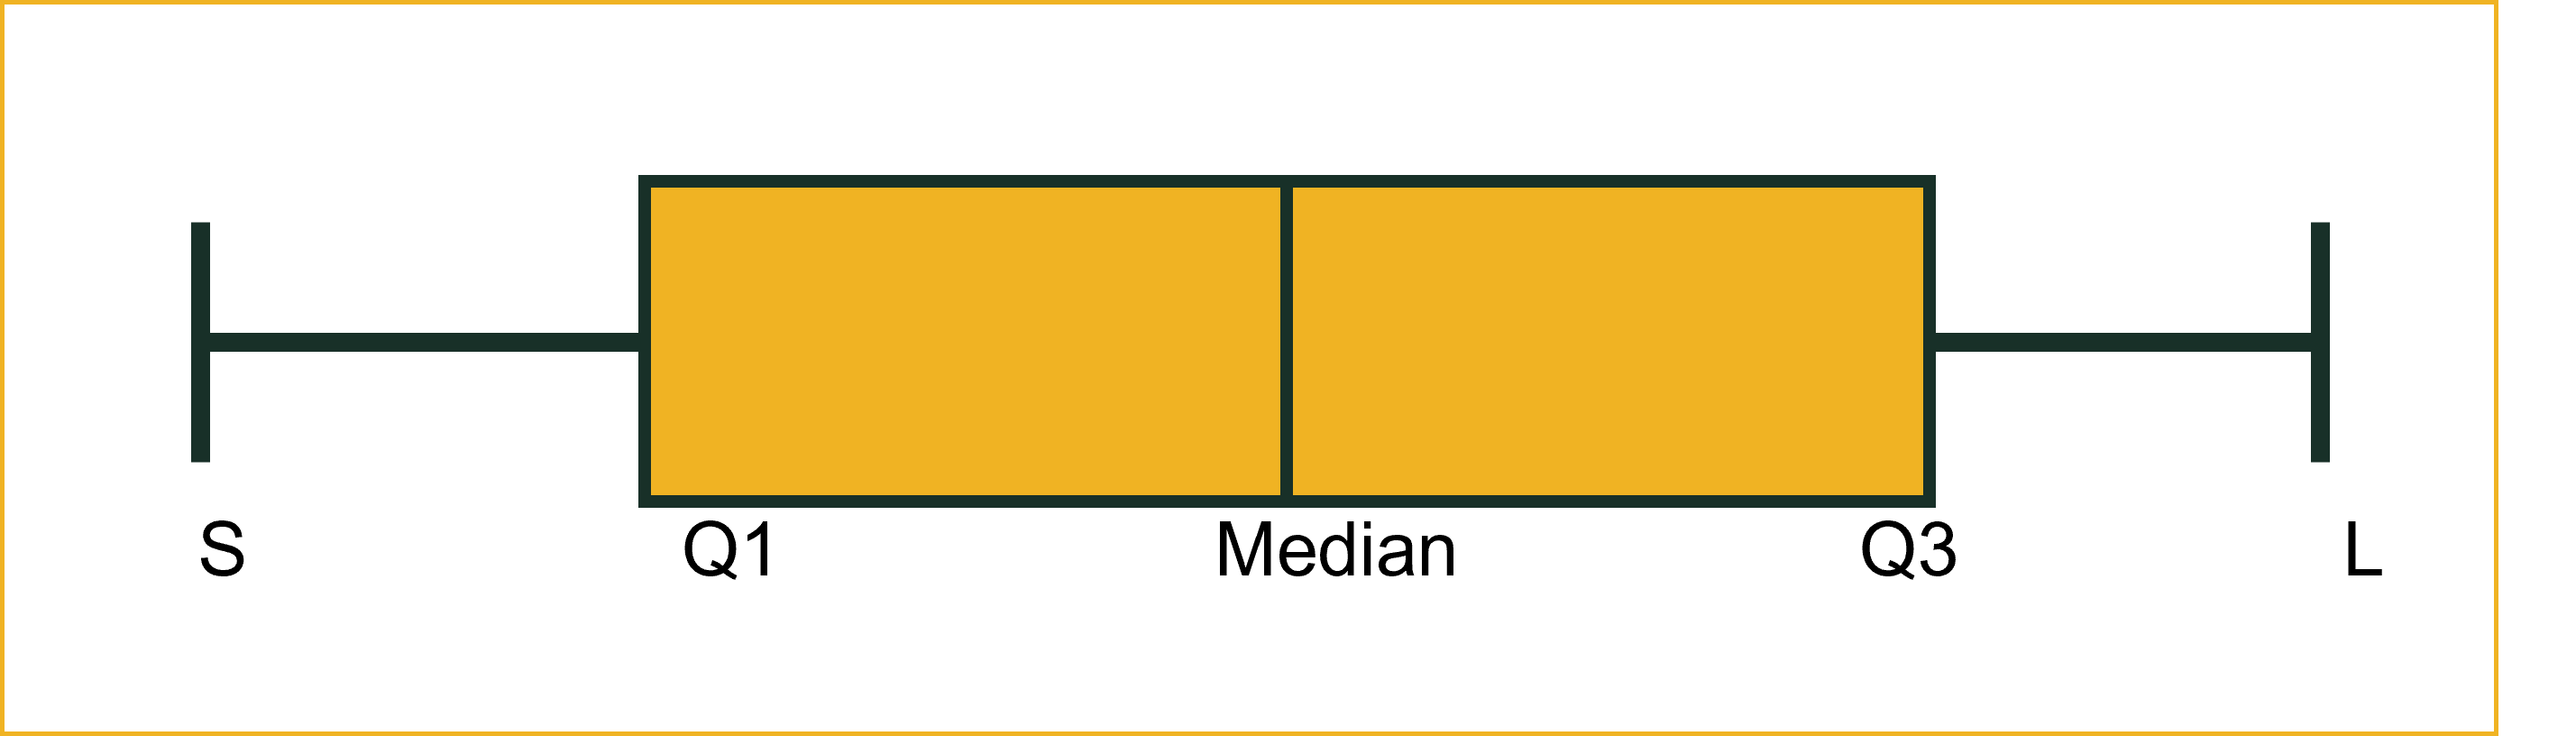
\includegraphics{Pictures/Ch3/Boxplot2.png}

}

\caption{A Boxplot with No Outliers}

\end{figure}%

\begin{itemize}
\tightlist
\item
  This boxplot above displays 5 summary values:

  \begin{itemize}
  \tightlist
  \item
    S = smallest value.
  \item
    L = largest value.
  \item
    Q1 = first quantile = 25th percentile.
  \item
    Q2 = median = second quantile = 50th percentile.
  \item
    Q3 = third quantile = 75th percentile.
  \end{itemize}
\item
  For example, use the GrowthFund Vector from the last lesson. It is
  executed again below.
\end{itemize}

\begin{Shaded}
\begin{Highlighting}[]
\NormalTok{GrowthFund }\OtherTok{\textless{}{-}} \FunctionTok{c}\NormalTok{(}\SpecialCharTok{{-}}\FloatTok{38.32}\NormalTok{, }\FloatTok{1.71}\NormalTok{, }\FloatTok{3.17}\NormalTok{, }\FloatTok{5.99}\NormalTok{, }\FloatTok{12.56}\NormalTok{, }\FloatTok{13.47}\NormalTok{, }\FloatTok{16.89}\NormalTok{, }\FloatTok{16.96}\NormalTok{, }\FloatTok{32.16}\NormalTok{,}
    \FloatTok{36.29}\NormalTok{)}
\NormalTok{GrowthFund }\OtherTok{\textless{}{-}} \FunctionTok{as.data.frame}\NormalTok{(GrowthFund)}
\end{Highlighting}
\end{Shaded}

\begin{itemize}
\tightlist
\item
  The quantile() function returns the five point summary when no
  arguments are specified.
\end{itemize}

\begin{Shaded}
\begin{Highlighting}[]
\NormalTok{QuanData }\OtherTok{\textless{}{-}} \FunctionTok{quantile}\NormalTok{(GrowthFund}\SpecialCharTok{$}\NormalTok{GrowthFund)}
\NormalTok{QuanData}
\end{Highlighting}
\end{Shaded}

\begin{verbatim}
      0%      25%      50%      75%     100% 
-38.3200   3.8750  13.0150  16.9425  36.2900 
\end{verbatim}

\section{Detecting Outliers}\label{detecting-outliers}

\begin{itemize}
\tightlist
\item
  We see an outlier visually, but without the tool available, we can
  detect them through the statistics. First we calculate the IQR, which
  is just quarter 3 minus quarter 1.
\end{itemize}

\begin{Shaded}
\begin{Highlighting}[]
\FunctionTok{summary}\NormalTok{(GrowthFund}\SpecialCharTok{$}\NormalTok{GrowthFund)}
\end{Highlighting}
\end{Shaded}

\begin{verbatim}
   Min. 1st Qu.  Median    Mean 3rd Qu.    Max. 
-38.320   3.875  13.015  10.088  16.942  36.290 
\end{verbatim}

\begin{Shaded}
\begin{Highlighting}[]
\NormalTok{IQRvalue }\OtherTok{\textless{}{-}} \FloatTok{16.9425} \SpecialCharTok{{-}} \FloatTok{3.875}
\NormalTok{IQRvalue}
\end{Highlighting}
\end{Shaded}

\begin{verbatim}
[1] 13.0675
\end{verbatim}

\begin{Shaded}
\begin{Highlighting}[]
\NormalTok{IQRvalue }\OtherTok{\textless{}{-}} \FunctionTok{IQR}\NormalTok{(GrowthFund}\SpecialCharTok{$}\NormalTok{GrowthFund)}
\NormalTok{IQRvalue}
\end{Highlighting}
\end{Shaded}

\begin{verbatim}
[1] 13.0675
\end{verbatim}

\begin{itemize}
\tightlist
\item
  Then, multiply the IQR by 1.5.
\end{itemize}

\begin{Shaded}
\begin{Highlighting}[]
\NormalTok{OutlierValue }\OtherTok{\textless{}{-}}\NormalTok{ IQRvalue }\SpecialCharTok{*} \FloatTok{1.5}
\NormalTok{OutlierValue}
\end{Highlighting}
\end{Shaded}

\begin{verbatim}
[1] 19.60125
\end{verbatim}

\begin{itemize}
\tightlist
\item
  Finally conduct 2 checks to determine if outliers are past the low
  whisker and/or high whisker.

  \begin{itemize}
  \tightlist
  \item
    A TRUE value indicates that at least one outlier is present at the
    small end of the distribution.
  \item
    A FALSE value indicates that no outliers are at the high end of the
    distribution.
  \end{itemize}
\end{itemize}

\begin{Shaded}
\begin{Highlighting}[]
\NormalTok{QuanData}
\end{Highlighting}
\end{Shaded}

\begin{verbatim}
      0%      25%      50%      75%     100% 
-38.3200   3.8750  13.0150  16.9425  36.2900 
\end{verbatim}

\begin{Shaded}
\begin{Highlighting}[]
\NormalTok{QuanData[}\DecValTok{2}\NormalTok{] }\SpecialCharTok{{-}}\NormalTok{ QuanData[}\DecValTok{1}\NormalTok{] }\SpecialCharTok{\textgreater{}}\NormalTok{ OutlierValue}
\end{Highlighting}
\end{Shaded}

\begin{verbatim}
 25% 
TRUE 
\end{verbatim}

\begin{Shaded}
\begin{Highlighting}[]
\CommentTok{\# True indicating an outlier to the left}
\FloatTok{3.875} \SpecialCharTok{{-}} \SpecialCharTok{{-}}\FloatTok{38.32}  \CommentTok{\#42.195}
\end{Highlighting}
\end{Shaded}

\begin{verbatim}
[1] 42.195
\end{verbatim}

\begin{Shaded}
\begin{Highlighting}[]
\FloatTok{42.195} \SpecialCharTok{\textgreater{}} \FloatTok{19.60125}  \CommentTok{\#TRUE}
\end{Highlighting}
\end{Shaded}

\begin{verbatim}
[1] TRUE
\end{verbatim}

\begin{Shaded}
\begin{Highlighting}[]
\NormalTok{QuanData[}\DecValTok{4}\NormalTok{] }\SpecialCharTok{{-}}\NormalTok{ QuanData[}\DecValTok{5}\NormalTok{] }\SpecialCharTok{\textgreater{}}\NormalTok{ OutlierValue}
\end{Highlighting}
\end{Shaded}

\begin{verbatim}
  75% 
FALSE 
\end{verbatim}

\begin{Shaded}
\begin{Highlighting}[]
\CommentTok{\# False indicating no outlier to the right.}
\FloatTok{16.9425} \SpecialCharTok{{-}} \FloatTok{36.29}  \CommentTok{\#{-}19.3475}
\end{Highlighting}
\end{Shaded}

\begin{verbatim}
[1] -19.3475
\end{verbatim}

\begin{Shaded}
\begin{Highlighting}[]
\SpecialCharTok{{-}}\FloatTok{19.3475} \SpecialCharTok{\textgreater{}} \FloatTok{19.60125}  \CommentTok{\#FALSE }
\end{Highlighting}
\end{Shaded}

\begin{verbatim}
[1] FALSE
\end{verbatim}

\subsection{Boxplot}\label{boxplot-1}

\begin{itemize}
\tightlist
\item
  We can use ggplot to retrieve our graph and associated numbers.
\item
  The outlier is visually depicted on the graph as -38.32.
\end{itemize}

\begin{Shaded}
\begin{Highlighting}[]
\FunctionTok{ggplot}\NormalTok{(GrowthFund, }\FunctionTok{aes}\NormalTok{(GrowthFund)) }\SpecialCharTok{+} \FunctionTok{geom\_boxplot}\NormalTok{()}
\end{Highlighting}
\end{Shaded}

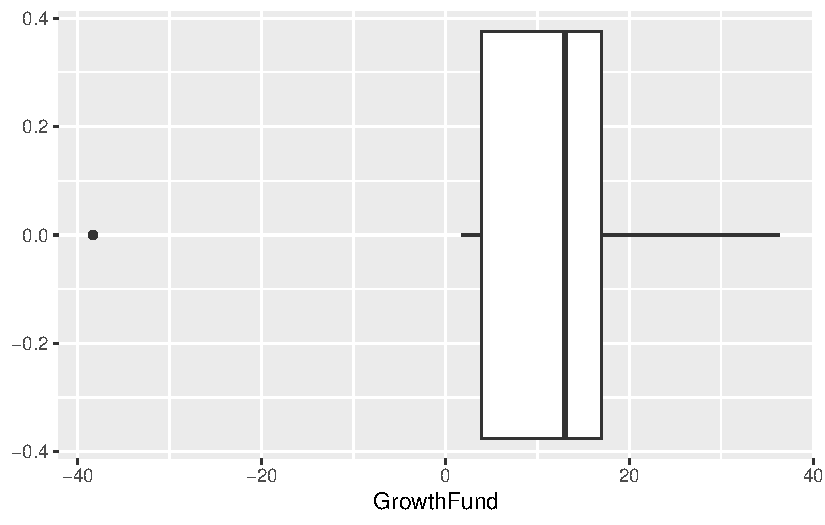
\includegraphics{dataviz_files/figure-pdf/unnamed-chunk-30-1.pdf}

\begin{itemize}
\tightlist
\item
  We can add a little color to the plot with the fill parameter, but
  then we also need to be sure to turn off the legends in the
  geom\_boxplot.
\end{itemize}

\begin{Shaded}
\begin{Highlighting}[]
\FunctionTok{ggplot}\NormalTok{(GrowthFund, }\FunctionTok{aes}\NormalTok{(GrowthFund, }\AttributeTok{fill =} \StringTok{"red"}\NormalTok{)) }\SpecialCharTok{+} \FunctionTok{geom\_boxplot}\NormalTok{(}\AttributeTok{show.legend =} \ConstantTok{FALSE}\NormalTok{)}
\end{Highlighting}
\end{Shaded}

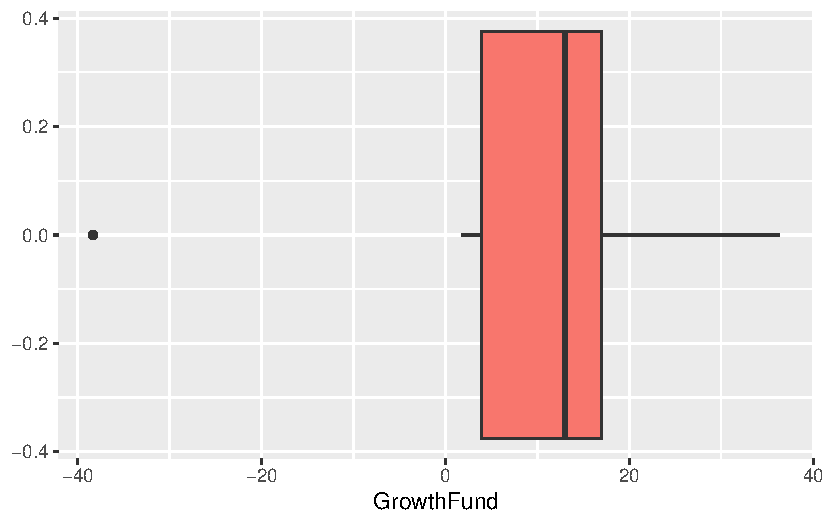
\includegraphics{dataviz_files/figure-pdf/unnamed-chunk-31-1.pdf}

\begin{itemize}
\tightlist
\item
  You can add parameters to make this visualization more professional,
  but this gets you started. Be sure to look at some examples in the R
  community or on ChatGPT.
\end{itemize}

\subsection{mtcars Example}\label{mtcars-example}

\begin{itemize}
\tightlist
\item
  We can also view mpg from the mtcars data set as a boxplot.
\item
  In this example, there is one outlier to the right.
\end{itemize}

\begin{Shaded}
\begin{Highlighting}[]
\FunctionTok{data}\NormalTok{(}\StringTok{"mtcars"}\NormalTok{)}
\FunctionTok{ggplot}\NormalTok{(mtcars, }\FunctionTok{aes}\NormalTok{(mpg)) }\SpecialCharTok{+} \FunctionTok{geom\_boxplot}\NormalTok{(}\AttributeTok{color=}\StringTok{"\#AAAAAA"}\NormalTok{, }\AttributeTok{fill=}\StringTok{"\#AAA3F3"}\NormalTok{) }\SpecialCharTok{+} \FunctionTok{theme\_minimal}\NormalTok{()}
\end{Highlighting}
\end{Shaded}

\includegraphics{dataviz_files/figure-pdf/unnamed-chunk-32-1.pdf}

\begin{itemize}
\tightlist
\item
  Let's get some summary statistics to check for outliers, skewness, and
  kurtosis to see how our visual aids help us in understanding those
  results.
\end{itemize}

\begin{Shaded}
\begin{Highlighting}[]
\NormalTok{IQRvalue }\OtherTok{\textless{}{-}} \FunctionTok{IQR}\NormalTok{(mtcars}\SpecialCharTok{$}\NormalTok{mpg)}
\NormalTok{OutlierValue }\OtherTok{\textless{}{-}}\NormalTok{ IQRvalue }\SpecialCharTok{*} \FloatTok{1.5}
\NormalTok{OutlierValue}
\end{Highlighting}
\end{Shaded}

\begin{verbatim}
[1] 11.0625
\end{verbatim}

\begin{Shaded}
\begin{Highlighting}[]
\NormalTok{QuanData }\OtherTok{\textless{}{-}} \FunctionTok{quantile}\NormalTok{(mtcars}\SpecialCharTok{$}\NormalTok{mpg)}
\NormalTok{QuanData}
\end{Highlighting}
\end{Shaded}

\begin{verbatim}
    0%    25%    50%    75%   100% 
10.400 15.425 19.200 22.800 33.900 
\end{verbatim}

\begin{Shaded}
\begin{Highlighting}[]
\NormalTok{QuanData[}\DecValTok{2}\NormalTok{] }\SpecialCharTok{{-}}\NormalTok{ QuanData[}\DecValTok{1}\NormalTok{] }\SpecialCharTok{\textgreater{}}\NormalTok{ OutlierValue}
\end{Highlighting}
\end{Shaded}

\begin{verbatim}
  25% 
FALSE 
\end{verbatim}

\begin{Shaded}
\begin{Highlighting}[]
\CommentTok{\# False indicating no outlier to the left}
\NormalTok{QuanData[}\DecValTok{4}\NormalTok{] }\SpecialCharTok{{-}}\NormalTok{ QuanData[}\DecValTok{5}\NormalTok{] }\SpecialCharTok{\textgreater{}}\NormalTok{ OutlierValue}
\end{Highlighting}
\end{Shaded}

\begin{verbatim}
  75% 
FALSE 
\end{verbatim}

\begin{Shaded}
\begin{Highlighting}[]
\CommentTok{\# False indicating no outlier to the right.}
\NormalTok{semTools}\SpecialCharTok{::}\FunctionTok{skew}\NormalTok{(mtcars}\SpecialCharTok{$}\NormalTok{mpg)}
\end{Highlighting}
\end{Shaded}

\begin{verbatim}
skew (g1)        se         z         p 
0.6723771 0.4330127 1.5527885 0.1204737 
\end{verbatim}

\begin{Shaded}
\begin{Highlighting}[]
\NormalTok{semTools}\SpecialCharTok{::}\FunctionTok{kurtosis}\NormalTok{(mtcars}\SpecialCharTok{$}\NormalTok{mpg)}
\end{Highlighting}
\end{Shaded}

\begin{verbatim}
Excess Kur (g2)              se               z               p 
    -0.02200629      0.86602540     -0.02541068      0.97972740 
\end{verbatim}

\begin{itemize}
\item
  Looks like the mpg variable is quite normal with no signs of outliers,
  skewness, or kurtosis. In the boxplot, it looks like there might be an
  outlier to the right, but it is not problematic to the dataset as
  indicated by the manual calculations.
\item
  We can also get a histogram of mpg and are able to make the same
  claims towards normality. You can see a slight pull to the right, but
  it is seemingly normal.
\end{itemize}

\begin{Shaded}
\begin{Highlighting}[]
\FunctionTok{ggplot}\NormalTok{(mtcars, }\FunctionTok{aes}\NormalTok{(mpg)) }\SpecialCharTok{+} \FunctionTok{geom\_histogram}\NormalTok{(}\AttributeTok{binwidth =} \DecValTok{5}\NormalTok{, }\AttributeTok{color =} \StringTok{"black"}\NormalTok{,}
    \AttributeTok{fill =} \StringTok{"green"}\NormalTok{)}
\end{Highlighting}
\end{Shaded}

\includegraphics{dataviz_files/figure-pdf/unnamed-chunk-34-1.pdf}

\bookmarksetup{startatroot}

\chapter{Graphs for Two Variables At
Once}\label{graphs-for-two-variables-at-once}

\begin{itemize}
\tightlist
\item
  Combinations of 2 Variable Types for Graphing

  \begin{itemize}
  \tightlist
  \item
    Two categorical/ factor.
  \item
    One categorical/ factor and one continuous/ numeric.
  \item
    Two continuous/ numeric.
  \end{itemize}
\end{itemize}

\section{Bar Graphs for Two Categorical
Variables}\label{bar-graphs-for-two-categorical-variables}

\begin{itemize}
\tightlist
\item
  There are two formats available for bar charts:

  \begin{itemize}
  \tightlist
  \item
    Grouped
  \item
    Stacked
  \end{itemize}
\end{itemize}

\begin{verbatim}
# A tibble: 6 x 3
# Groups:   vs, gear [6]
     vs  gear     n
  <dbl> <dbl> <int>
1     0     3    12
2     0     4     2
3     0     5     4
4     1     3     3
5     1     4    10
6     1     5     1
\end{verbatim}

\includegraphics{dataviz_files/figure-pdf/unnamed-chunk-35-1.pdf}

\includegraphics{dataviz_files/figure-pdf/unnamed-chunk-35-2.pdf}

\subsection{Grouped Bar Graph}\label{grouped-bar-graph}

\begin{itemize}
\tightlist
\item
  Grouped bar graph allow comparison of multiple sets of data items,
  with a single color used to denote a specific series across all sets.
\item
  For example, we can look at both the vs and gear variables in the
  ggplot command.

  \begin{itemize}
  \tightlist
  \item
    We did a little grouping and counting before we began to generate a
    new table with frequencies based on vs and gear variables.
  \item
    Once the dataset was made, we can make the graph with the geom\_bar
    layer.
  \item
    Since there are two variables, we need to set the position to dodge.
  \item
    (stat = ``identity'') tells ggplot that the y values are already
    computed and should be used as-is for the heights of the bars. In
    this case, they are frequencies calculated in the countsDF dataset.
  \end{itemize}
\end{itemize}

\begin{Shaded}
\begin{Highlighting}[]
\NormalTok{mtcars }\OtherTok{\textless{}{-}}\NormalTok{ mtcars }\SpecialCharTok{\%\textgreater{}\%}
    \FunctionTok{mutate}\NormalTok{(}\AttributeTok{vs =} \FunctionTok{as.factor}\NormalTok{(vs)) }\SpecialCharTok{\%\textgreater{}\%}
    \FunctionTok{mutate}\NormalTok{(}\AttributeTok{gear =} \FunctionTok{as.factor}\NormalTok{(gear))}


\NormalTok{countsDF }\OtherTok{\textless{}{-}}\NormalTok{ mtcars }\SpecialCharTok{\%\textgreater{}\%}
    \FunctionTok{group\_by}\NormalTok{(vs, gear) }\SpecialCharTok{\%\textgreater{}\%}
    \FunctionTok{count}\NormalTok{()}

\FunctionTok{summary}\NormalTok{(countsDF)}
\end{Highlighting}
\end{Shaded}

\begin{verbatim}
 vs    gear        n         
 0:3   3:2   Min.   : 1.000  
 1:3   4:2   1st Qu.: 2.250  
       5:2   Median : 3.500  
             Mean   : 5.333  
             3rd Qu.: 8.500  
             Max.   :12.000  
\end{verbatim}

\begin{Shaded}
\begin{Highlighting}[]
\FunctionTok{ggplot}\NormalTok{(countsDF, }\FunctionTok{aes}\NormalTok{(}\AttributeTok{x =}\NormalTok{ gear, }\AttributeTok{y =}\NormalTok{ n, }\AttributeTok{fill =}\NormalTok{ vs)) }\SpecialCharTok{+} \FunctionTok{geom\_bar}\NormalTok{(}\AttributeTok{stat =} \StringTok{"identity"}\NormalTok{,}
    \AttributeTok{position =} \StringTok{"dodge"}\NormalTok{) }\SpecialCharTok{+} \FunctionTok{labs}\NormalTok{(}\AttributeTok{title =} \StringTok{"Grouped Car Distribution by Gears and VS"}\NormalTok{,}
    \AttributeTok{x =} \StringTok{"Number of Gears"}\NormalTok{, }\AttributeTok{y =} \StringTok{"Count"}\NormalTok{) }\SpecialCharTok{+} \FunctionTok{theme\_minimal}\NormalTok{()}
\end{Highlighting}
\end{Shaded}

\includegraphics{dataviz_files/figure-pdf/unnamed-chunk-36-1.pdf}

\subsection{Stacked Bar Graph}\label{stacked-bar-graph}

\begin{itemize}
\tightlist
\item
  A Stacked bar graph extends the standard bar graph from looking at
  numeric values across one categorical variable to two. Each bar in a
  standard bar graph is divided into a number of sub-bars stacked end to
  end, each one corresponding to a level of the second categorical
  variable.
\item
  Using ggplot, we can also stack these charts by removing the position
  = dodge statement.
\end{itemize}

\begin{Shaded}
\begin{Highlighting}[]
\FunctionTok{ggplot}\NormalTok{(countsDF, }\FunctionTok{aes}\NormalTok{(}\AttributeTok{x =}\NormalTok{ gear, }\AttributeTok{y =}\NormalTok{ n, }\AttributeTok{fill =}\NormalTok{ vs)) }\SpecialCharTok{+}
  \FunctionTok{geom\_bar}\NormalTok{(}\AttributeTok{stat =} \StringTok{"identity"}\NormalTok{, }\AttributeTok{position =} \StringTok{"dodge"}\NormalTok{) }\SpecialCharTok{+}
  \FunctionTok{labs}\NormalTok{(}\AttributeTok{title =} \StringTok{"Stacked Car Distribution"}\NormalTok{,}
       \AttributeTok{x =} \StringTok{"Number of Gears"}\NormalTok{,}
       \AttributeTok{y =} \StringTok{"Count"}\NormalTok{) }\SpecialCharTok{+}
  \FunctionTok{theme\_minimal}\NormalTok{()}
\end{Highlighting}
\end{Shaded}

\includegraphics{dataviz_files/figure-pdf/unnamed-chunk-37-1.pdf}

\section{Bar Graph for Continuous Across
Groups}\label{bar-graph-for-continuous-across-groups}

\begin{itemize}
\item
  In comparison to a bar graph for a single categorical variable, a bar
  chart for a continuous variable across groups includes both a x and y
  axis. The continuous variable is put on the y axis, and the
  categorical (factor) variable is placed on the x axis showing the
  groups.
\item
  Therefore, instead of counting data based on group, we can see another
  continuous variable based on group data.
\item
  The frequency data (i.e., counts) can be replaced with another
  numerical variable like mean.
\item
  In the below example, instead of counting observations per group,
  here, we took the average mpg (a continuous variable) based on groups
  of gear and vs and summarized the data into a variable avg\_mpg. We
  then used that variable in a ggplot() command to create a unique chart
  to that above.
\end{itemize}

\begin{Shaded}
\begin{Highlighting}[]
\NormalTok{avg\_mpg }\OtherTok{\textless{}{-}}\NormalTok{ mtcars }\SpecialCharTok{\%\textgreater{}\%}
    \FunctionTok{group\_by}\NormalTok{(gear, vs) }\SpecialCharTok{\%\textgreater{}\%}
    \FunctionTok{summarise}\NormalTok{(}\AttributeTok{mpg =} \FunctionTok{mean}\NormalTok{(mpg, }\AttributeTok{na.rm =} \ConstantTok{TRUE}\NormalTok{))}
\end{Highlighting}
\end{Shaded}

\begin{Shaded}
\begin{Highlighting}[]
\FunctionTok{ggplot}\NormalTok{(avg\_mpg, }\FunctionTok{aes}\NormalTok{(gear,}
\NormalTok{  mpg, }\AttributeTok{fill =}\NormalTok{ vs)) }\SpecialCharTok{+}
  \FunctionTok{geom\_bar}\NormalTok{(}\AttributeTok{stat =} \StringTok{"identity"}\NormalTok{, }\AttributeTok{position =} \StringTok{"dodge"}\NormalTok{) }\SpecialCharTok{+}
  \FunctionTok{ggtitle}\NormalTok{(}\StringTok{"Average MPG by VS and Gear"}\NormalTok{)}
\end{Highlighting}
\end{Shaded}

\includegraphics{dataviz_files/figure-pdf/unnamed-chunk-39-1.pdf}

\begin{itemize}
\tightlist
\item
  We can add color using the scale\_fill\_manual. Since there are two
  colors, we use the c() command to combine them together inside the
  layer.

  \begin{itemize}
  \tightlist
  \item
    scale\_fill\_manual() is a function used to manually set the colors
    for filled areas (like bars, areas in geom\_area, etc.) in a plot.
    Here, values argument takes our custom color palette of yellow and
    brown.
  \end{itemize}
\end{itemize}

\begin{Shaded}
\begin{Highlighting}[]
\FunctionTok{ggplot}\NormalTok{(avg\_mpg, }\FunctionTok{aes}\NormalTok{(gear, mpg, }\AttributeTok{fill =}\NormalTok{ vs)) }\SpecialCharTok{+} \FunctionTok{geom\_bar}\NormalTok{(}\AttributeTok{stat =} \StringTok{"identity"}\NormalTok{,}
    \AttributeTok{position =} \StringTok{"dodge"}\NormalTok{, }\AttributeTok{color =} \StringTok{"black"}\NormalTok{) }\SpecialCharTok{+} \FunctionTok{ggtitle}\NormalTok{(}\StringTok{"Average MPG by VS and Gear"}\NormalTok{) }\SpecialCharTok{+}
    \FunctionTok{scale\_fill\_manual}\NormalTok{(}\AttributeTok{values =} \FunctionTok{c}\NormalTok{(}\StringTok{"yellow"}\NormalTok{, }\StringTok{"brown"}\NormalTok{))}
\end{Highlighting}
\end{Shaded}

\includegraphics{dataviz_files/figure-pdf/unnamed-chunk-40-1.pdf}

\subsection{Boxplot for Continuous Across
Groups}\label{boxplot-for-continuous-across-groups}

\begin{itemize}
\item
  A boxplot requires one continuous variable (like we did above). When
  we include an additional grouping variable, we get multiple boxplots,
  one for each group. This allows us to directly compare distributions.
\item
  The categorical variable should correctly be a factor data type before
  you begin.
\item
  In the example below, mpg is the continuous variable, and gear is the
  categorical variable.
\item
  We see 3 boxplots for three values of gear (3, 4, 5). ggplot() and
  geom\_boxplot() are required components of the command. The
  scale\_fill\_manual() and theme\_minimal() layers are optional ways to
  change the style and color.
\end{itemize}

\begin{Shaded}
\begin{Highlighting}[]
\NormalTok{mtcars }\SpecialCharTok{\%\textgreater{}\%}
  \FunctionTok{ggplot}\NormalTok{(}\FunctionTok{aes}\NormalTok{(}\AttributeTok{x =}\NormalTok{ gear, }\AttributeTok{y =}\NormalTok{ mpg)) }\SpecialCharTok{+}
  \FunctionTok{geom\_boxplot}\NormalTok{(}\FunctionTok{aes}\NormalTok{(}\AttributeTok{fill =}\NormalTok{ gear)) }\SpecialCharTok{+}
  \FunctionTok{scale\_fill\_manual}\NormalTok{(}\AttributeTok{values =} \FunctionTok{c}\NormalTok{(}\StringTok{"gray"}\NormalTok{, }\StringTok{"red"}\NormalTok{, }\StringTok{"blue"}\NormalTok{)) }\SpecialCharTok{+}
  \FunctionTok{theme\_minimal}\NormalTok{()}
\end{Highlighting}
\end{Shaded}

\includegraphics{dataviz_files/figure-pdf/unnamed-chunk-41-1.pdf}

\begin{itemize}
\tightlist
\item
  Lets alter the functions above to depict mpg based on vs with
  categorical states 0 and 1.
\end{itemize}

\begin{Shaded}
\begin{Highlighting}[]
\NormalTok{mtcars }\SpecialCharTok{\%\textgreater{}\%}
    \FunctionTok{ggplot}\NormalTok{(}\FunctionTok{aes}\NormalTok{(}\AttributeTok{x =}\NormalTok{ vs, }\AttributeTok{y =}\NormalTok{ mpg)) }\SpecialCharTok{+} \FunctionTok{geom\_boxplot}\NormalTok{(}\FunctionTok{aes}\NormalTok{(}\AttributeTok{fill =}\NormalTok{ vs), }\AttributeTok{show.legend =} \ConstantTok{FALSE}\NormalTok{) }\SpecialCharTok{+}
    \FunctionTok{scale\_fill\_manual}\NormalTok{(}\AttributeTok{values =} \FunctionTok{c}\NormalTok{(}\StringTok{"gray"}\NormalTok{, }\StringTok{"red"}\NormalTok{)) }\SpecialCharTok{+} \FunctionTok{theme\_minimal}\NormalTok{()}
\end{Highlighting}
\end{Shaded}

\includegraphics{dataviz_files/figure-pdf/unnamed-chunk-42-1.pdf}

\section{Graphs for Two Continuous
Variables}\label{graphs-for-two-continuous-variables}

\subsection{Scatterplots}\label{scatterplots}

\begin{itemize}
\tightlist
\item
  A scatterplot is used to determine if two continuous variables are
  related.

  \begin{itemize}
  \tightlist
  \item
    Each point is a pairing: \((x_1, y_1),(x_2, y_2),\) etc.
  \end{itemize}
\item
  Our goal with a scatterplot is to characterize the relationship by
  visual inspection. This includes determining if the relationship looks
  positive, negative, or not existent.
\end{itemize}

\begin{figure}[H]

{\centering \includegraphics{Pictures/Ch3/Scatter.png}

}

\caption{ScatterPlot Results}

\end{figure}%

\begin{itemize}
\item
  Sometimes, it is really clear how to characterize the relationship.
  Other times, additional statistical tests are needed to confirm the
  relationship (which we will go over in later lessons). This is true
  especially with big data, where the plot window can look like a giant
  blog of observations.
\item
  Let's work a clean example examining the relationship between income
  and the years of education one has had.
\item
  This plot has a clear positive trend, meaning that as one has more
  years of education, we see higher income. And similarly, as we see
  higher income, we also see more years of education. This means that a
  scatter can help characterize the relationship, and does \emph{not}
  state that one variable is causing another to occur.
\end{itemize}

\begin{Shaded}
\begin{Highlighting}[]
\NormalTok{Edu }\OtherTok{\textless{}{-}} \FunctionTok{read.csv}\NormalTok{(}\StringTok{"data/education.csv"}\NormalTok{)}
\FunctionTok{plot}\NormalTok{(Edu}\SpecialCharTok{$}\NormalTok{Income }\SpecialCharTok{\textasciitilde{}}\NormalTok{ Edu}\SpecialCharTok{$}\NormalTok{Education, }\AttributeTok{ylab =} \StringTok{"Income"}\NormalTok{, }\AttributeTok{xlab =} \StringTok{"Education"}\NormalTok{)}
\end{Highlighting}
\end{Shaded}

\includegraphics{dataviz_files/figure-pdf/unnamed-chunk-44-1.pdf}

\begin{itemize}
\tightlist
\item
  Working with ggplot instead of base R, we would use the following
  code.

  \begin{itemize}
  \tightlist
  \item
    Layer 1: ggplot() command with aes() command directly inside of it
    pointing to x and y variables.
  \item
    Layer 2: geom\_point() command to add the observations as indicators
    in the chart.
  \item
    Layer 3 or more: many other optional additions like labs (for
    labels) as shown below.
  \end{itemize}
\end{itemize}

\begin{Shaded}
\begin{Highlighting}[]
\FunctionTok{ggplot}\NormalTok{(Edu, }\FunctionTok{aes}\NormalTok{(}\AttributeTok{x =}\NormalTok{ Education, }\AttributeTok{y =}\NormalTok{ Income)) }\SpecialCharTok{+} \FunctionTok{geom\_point}\NormalTok{() }\SpecialCharTok{+} \FunctionTok{labs}\NormalTok{(}\AttributeTok{y =} \StringTok{"Income"}\NormalTok{,}
    \AttributeTok{x =} \StringTok{"Education"}\NormalTok{)}
\end{Highlighting}
\end{Shaded}

\includegraphics{dataviz_files/figure-pdf/unnamed-chunk-45-1.pdf}

\begin{itemize}
\tightlist
\item
  geom\_point() has some parameters you can change like shape = where
  you can add depth to your chart. Some common shapes of geom\_point are
  as follows.
\end{itemize}

\begin{Shaded}
\begin{Highlighting}[]
\CommentTok{\# shape = 0, square shape = 1, circle shape = 2, triangle point up}
\CommentTok{\# shape = 3, plus shape = 4, cross shape = 5, diamond shape = 6,}
\CommentTok{\# triangle point down shape = 7, square cross shape = 8, star shape =}
\CommentTok{\# 9, diamond plus shape = 10, circle plus shape = 11, triangles up}
\CommentTok{\# and down shape = 12, square plus shape = 13, circle cross shape =}
\CommentTok{\# 14, square and triangle down shape = 15, filled square shape = 16,}
\CommentTok{\# filled circle shape = 17, filled triangle point{-}up shape = 18,}
\CommentTok{\# filled diamond}
\end{Highlighting}
\end{Shaded}

\begin{itemize}
\tightlist
\item
  For instance, the code below changes the color, shape, and size of the
  geom\_point().
\end{itemize}

\begin{Shaded}
\begin{Highlighting}[]
\FunctionTok{ggplot}\NormalTok{(Edu, }\FunctionTok{aes}\NormalTok{(}\AttributeTok{x =}\NormalTok{ Education, }\AttributeTok{y =}\NormalTok{ Income)) }\SpecialCharTok{+} \FunctionTok{geom\_point}\NormalTok{(}\AttributeTok{color =} \StringTok{"\#183028"}\NormalTok{,}
    \AttributeTok{shape =} \DecValTok{18}\NormalTok{, }\AttributeTok{size =} \DecValTok{10}\NormalTok{) }\SpecialCharTok{+} \FunctionTok{labs}\NormalTok{(}\AttributeTok{y =} \StringTok{"Income"}\NormalTok{, }\AttributeTok{x =} \StringTok{"Education"}\NormalTok{)}
\end{Highlighting}
\end{Shaded}

\includegraphics{dataviz_files/figure-pdf/unnamed-chunk-47-1.pdf}

\begin{itemize}
\tightlist
\item
  ggplot allows us to add a geom\_line, which is helpful in drawing a
  line through the data. Here, I am also resetting the color off of the
  default value. You see this a lot on time series models like stock
  charts.
\end{itemize}

\begin{Shaded}
\begin{Highlighting}[]
\FunctionTok{ggplot}\NormalTok{(Edu, }\FunctionTok{aes}\NormalTok{(}\AttributeTok{x =}\NormalTok{ Education, }\AttributeTok{y =}\NormalTok{ Income)) }\SpecialCharTok{+} \FunctionTok{geom\_point}\NormalTok{(}\AttributeTok{color =} \StringTok{"\#183028"}\NormalTok{,}
    \AttributeTok{shape =} \DecValTok{18}\NormalTok{, }\AttributeTok{size =} \DecValTok{4}\NormalTok{) }\SpecialCharTok{+} \FunctionTok{labs}\NormalTok{(}\AttributeTok{y =} \StringTok{"Income"}\NormalTok{, }\AttributeTok{x =} \StringTok{"Education"}\NormalTok{) }\SpecialCharTok{+} \FunctionTok{geom\_line}\NormalTok{(}\AttributeTok{color =} \StringTok{"\#789F90"}\NormalTok{)}
\end{Highlighting}
\end{Shaded}

\includegraphics{dataviz_files/figure-pdf/unnamed-chunk-48-1.pdf}

\begin{itemize}
\tightlist
\item
  Another way to do this is to add a stat\_smooth line, which is
  considered a trendline to help us visualize the relationship between
  the variables.
\end{itemize}

\begin{Shaded}
\begin{Highlighting}[]
\FunctionTok{ggplot}\NormalTok{(Edu, }\FunctionTok{aes}\NormalTok{(}\AttributeTok{x =}\NormalTok{ Education, }\AttributeTok{y =}\NormalTok{ Income)) }\SpecialCharTok{+} \FunctionTok{geom\_point}\NormalTok{(}\AttributeTok{color =} \StringTok{"\#183028"}\NormalTok{,}
    \AttributeTok{shape =} \DecValTok{18}\NormalTok{, }\AttributeTok{size =} \DecValTok{4}\NormalTok{) }\SpecialCharTok{+} \FunctionTok{labs}\NormalTok{(}\AttributeTok{y =} \StringTok{"Income"}\NormalTok{, }\AttributeTok{x =} \StringTok{"Education"}\NormalTok{) }\SpecialCharTok{+} \FunctionTok{stat\_smooth}\NormalTok{(}\AttributeTok{color =} \StringTok{"\#789F90"}\NormalTok{)}
\end{Highlighting}
\end{Shaded}

\includegraphics{dataviz_files/figure-pdf/unnamed-chunk-49-1.pdf}

\begin{itemize}
\tightlist
\item
  We can change the type of trendline. The most common is the to develop
  the trendline using the lm method, which stands for the linear method
  that we are going to learn in Chapter 9. For now, lets insert
  \_method=``lm'' into our stat\_smooth later to see the change.
\end{itemize}

\begin{Shaded}
\begin{Highlighting}[]
\FunctionTok{ggplot}\NormalTok{(Edu, }\FunctionTok{aes}\NormalTok{(}\AttributeTok{x =}\NormalTok{ Education, }\AttributeTok{y =}\NormalTok{ Income)) }\SpecialCharTok{+} \FunctionTok{geom\_point}\NormalTok{() }\SpecialCharTok{+} \FunctionTok{labs}\NormalTok{(}\AttributeTok{y =} \StringTok{"Income"}\NormalTok{,}
    \AttributeTok{x =} \StringTok{"Education"}\NormalTok{) }\SpecialCharTok{+} \FunctionTok{stat\_smooth}\NormalTok{(}\AttributeTok{method =} \StringTok{"lm"}\NormalTok{, }\AttributeTok{color =} \StringTok{"\#789F90"}\NormalTok{)}
\end{Highlighting}
\end{Shaded}

\includegraphics{dataviz_files/figure-pdf/unnamed-chunk-50-1.pdf}

\begin{itemize}
\tightlist
\item
  Let's look at a few more examples and see if the relationship is
  considered positive, negative, or not existent.
\item
  Below, we see a negative trend.
\end{itemize}

\begin{Shaded}
\begin{Highlighting}[]
\FunctionTok{ggplot}\NormalTok{(mtcars, }\FunctionTok{aes}\NormalTok{(}\AttributeTok{x =}\NormalTok{ disp, }\AttributeTok{y =}\NormalTok{ mpg)) }\SpecialCharTok{+} \FunctionTok{geom\_point}\NormalTok{() }\SpecialCharTok{+} \FunctionTok{stat\_smooth}\NormalTok{(}\AttributeTok{method =} \StringTok{"lm"}\NormalTok{,}
    \AttributeTok{color =} \StringTok{"\#789F90"}\NormalTok{)}
\end{Highlighting}
\end{Shaded}

\includegraphics{dataviz_files/figure-pdf/unnamed-chunk-51-1.pdf}

\begin{itemize}
\tightlist
\item
  In regards to hp, below, we see another negative trend.
\end{itemize}

\begin{Shaded}
\begin{Highlighting}[]
\FunctionTok{ggplot}\NormalTok{(mtcars, }\FunctionTok{aes}\NormalTok{(}\AttributeTok{x =}\NormalTok{ hp, }\AttributeTok{y =}\NormalTok{ mpg)) }\SpecialCharTok{+} \FunctionTok{geom\_point}\NormalTok{() }\SpecialCharTok{+} \FunctionTok{stat\_smooth}\NormalTok{(}\AttributeTok{method =} \StringTok{"lm"}\NormalTok{,}
    \AttributeTok{color =} \StringTok{"\#789F90"}\NormalTok{)}
\end{Highlighting}
\end{Shaded}

\includegraphics{dataviz_files/figure-pdf/unnamed-chunk-52-1.pdf}

\begin{itemize}
\tightlist
\item
  In regards to qsec, below, we see a weak positive trend. This
  relationship would need to verified later on.
\end{itemize}

\begin{Shaded}
\begin{Highlighting}[]
\FunctionTok{ggplot}\NormalTok{(mtcars, }\FunctionTok{aes}\NormalTok{(}\AttributeTok{x =}\NormalTok{ qsec, }\AttributeTok{y =}\NormalTok{ mpg)) }\SpecialCharTok{+} \FunctionTok{geom\_point}\NormalTok{() }\SpecialCharTok{+} \FunctionTok{stat\_smooth}\NormalTok{(}\AttributeTok{method =} \StringTok{"lm"}\NormalTok{,}
    \AttributeTok{color =} \StringTok{"\#789F90"}\NormalTok{)}
\end{Highlighting}
\end{Shaded}

\includegraphics{dataviz_files/figure-pdf/unnamed-chunk-53-1.pdf}

\begin{itemize}
\tightlist
\item
  The plot() command also works when you do not have 2 continuous
  variables, and instead have one categorical variable paired with one
  continuous variable. However, the plot is not as adequate as others
  are in inferring the relationship from the variables.
\item
  For example, the plot below would be better served as a boxplot.
\end{itemize}

\begin{Shaded}
\begin{Highlighting}[]
\FunctionTok{plot}\NormalTok{(mtcars}\SpecialCharTok{$}\NormalTok{mpg }\SpecialCharTok{\textasciitilde{}}\NormalTok{ mtcars}\SpecialCharTok{$}\NormalTok{vs)}
\FunctionTok{boxplot}\NormalTok{(mtcars}\SpecialCharTok{$}\NormalTok{mpg }\SpecialCharTok{\textasciitilde{}}\NormalTok{ mtcars}\SpecialCharTok{$}\NormalTok{vs)}
\end{Highlighting}
\end{Shaded}

\includegraphics{dataviz_files/figure-pdf/unnamed-chunk-54-1.pdf}

\begin{itemize}
\tightlist
\item
  Using ggplot, we would have the same issue. Since vs is categorical,
  it does not look right when we use the geom\_point() later.
\end{itemize}

\begin{Shaded}
\begin{Highlighting}[]
\FunctionTok{ggplot}\NormalTok{(mtcars, }\FunctionTok{aes}\NormalTok{(}\AttributeTok{x =}\NormalTok{ vs, }\AttributeTok{y =}\NormalTok{ mpg)) }\SpecialCharTok{+} \FunctionTok{geom\_point}\NormalTok{() }\SpecialCharTok{+} \FunctionTok{stat\_smooth}\NormalTok{(}\AttributeTok{method =} \StringTok{"lm"}\NormalTok{)}
\end{Highlighting}
\end{Shaded}

\includegraphics{dataviz_files/figure-pdf/unnamed-chunk-55-1.pdf}

\begin{itemize}
\tightlist
\item
  Instead, we would want the geom\_boxplot layer like shown below. The
  stat\_smooth() is also not an applicable layer to a boxplot and would
  need to be removed.
\end{itemize}

\begin{Shaded}
\begin{Highlighting}[]
\FunctionTok{ggplot}\NormalTok{(mtcars, }\FunctionTok{aes}\NormalTok{(}\AttributeTok{x =}\NormalTok{ vs, }\AttributeTok{y =}\NormalTok{ mpg)) }\SpecialCharTok{+} \FunctionTok{geom\_boxplot}\NormalTok{()}
\end{Highlighting}
\end{Shaded}

\includegraphics{dataviz_files/figure-pdf/unnamed-chunk-56-1.pdf}

\subsection{Try to Recreate}\label{try-to-recreate}

\begin{itemize}
\tightlist
\item
  You try examples of scatterplots using the UScrime data set that is
  part of the MASS package to examine a few relationships using ggplot2.
  A few examples are below.
\end{itemize}

\includegraphics{dataviz_files/figure-pdf/unnamed-chunk-57-1.pdf}

\includegraphics{dataviz_files/figure-pdf/unnamed-chunk-57-2.pdf}

\includegraphics{dataviz_files/figure-pdf/unnamed-chunk-57-3.pdf}

\includegraphics{dataviz_files/figure-pdf/unnamed-chunk-57-4.pdf}

\begin{itemize}
\tightlist
\item
  See what information you can take away from the scatterplots above and
  create some more to practice.
\end{itemize}

\bookmarksetup{startatroot}

\chapter{Full Example Using nhanes
Dataset}\label{full-example-using-nhanes-dataset}

\begin{itemize}
\tightlist
\item
  A big example of where charts are helpful is to explore the nhanes
  dataset, which is actually a dataset related to auditory issues, in
  which the number of guns fired is a variable.
\item
  Specifically, AUQ060 refers to ``Hear a whisper from across a quiet
  room?'' AUQ070 refers to ``Hear normal voice across a quiet room?''
  and AUQ080 refers to ``Hear a shout from across a quiet room?'' While
  AUQ300 refers to ``Ever used firearms for any reason? AUQ310 refers
  to''How many total rounds ever fired?'' and AUQ320 refers to ``Wear
  hearing protection when shooting?'' I got these references in the
  nhanes\_auditory\_2012\_codebook.html file.
\item
  It would be interesting to determine whether there is a relationship
  between hearing loss and gun use. Below, I clean the data set and make
  some charts. All variables are categorical, and I only look at 2
  categorical variables at a time - one auditory related (AUQ 060, 070,
  080) and one gun related (AUQ 300, 310, 320).
\item
  The first step is data cleaning, and in particular recoding the
  variables of interest. We did some of these before. Let's also filter
  out the unused variables using the select statement.\\
\item
  The select statement in dplyr has a conflict with the select statement
  in MASS. Since we used MASS earlier, we have to specify which package
  we want to use select from. We want to use select from dplyr, so we
  add dplyr:: before the function.
\end{itemize}

\begin{Shaded}
\begin{Highlighting}[]
\NormalTok{nhanes }\OtherTok{\textless{}{-}} \FunctionTok{read.csv}\NormalTok{(}\StringTok{"data/nhanes2012.csv"}\NormalTok{)}
\CommentTok{\# summary(nhanes)}

\NormalTok{nhanes.clean }\OtherTok{\textless{}{-}}\NormalTok{ nhanes }\SpecialCharTok{\%\textgreater{}\%}
\NormalTok{    dplyr}\SpecialCharTok{::}\FunctionTok{select}\NormalTok{(AUQ300, AUQ310, AUQ320, AUQ060, AUQ070, AUQ080) }\SpecialCharTok{\%\textgreater{}\%}
    \FunctionTok{mutate}\NormalTok{(}\AttributeTok{AUQ300 =} \FunctionTok{recode\_factor}\NormalTok{(AUQ300, }\StringTok{\textasciigrave{}}\AttributeTok{1}\StringTok{\textasciigrave{}} \OtherTok{=} \StringTok{"Yes"}\NormalTok{, }\StringTok{\textasciigrave{}}\AttributeTok{2}\StringTok{\textasciigrave{}} \OtherTok{=} \StringTok{"No"}\NormalTok{)) }\SpecialCharTok{\%\textgreater{}\%}
    \FunctionTok{mutate}\NormalTok{(}\AttributeTok{AUQ310 =} \FunctionTok{recode\_factor}\NormalTok{(AUQ310, }\StringTok{\textasciigrave{}}\AttributeTok{1}\StringTok{\textasciigrave{}} \OtherTok{=} \StringTok{"1 to less than 100"}\NormalTok{, }\StringTok{\textasciigrave{}}\AttributeTok{2}\StringTok{\textasciigrave{}} \OtherTok{=} \StringTok{"100 to less than 1000"}\NormalTok{,}
        \StringTok{\textasciigrave{}}\AttributeTok{3}\StringTok{\textasciigrave{}} \OtherTok{=} \StringTok{"1000 to less than 10k"}\NormalTok{, }\StringTok{\textasciigrave{}}\AttributeTok{4}\StringTok{\textasciigrave{}} \OtherTok{=} \StringTok{"10k to less than 50k"}\NormalTok{, }\StringTok{\textasciigrave{}}\AttributeTok{5}\StringTok{\textasciigrave{}} \OtherTok{=} \StringTok{"50k or more"}\NormalTok{,}
        \StringTok{\textasciigrave{}}\AttributeTok{7}\StringTok{\textasciigrave{}} \OtherTok{=} \StringTok{"Refused"}\NormalTok{, }\StringTok{\textasciigrave{}}\AttributeTok{9}\StringTok{\textasciigrave{}} \OtherTok{=} \StringTok{"Don\textquotesingle{}t know"}\NormalTok{)) }\SpecialCharTok{\%\textgreater{}\%}
    \FunctionTok{mutate}\NormalTok{(}\AttributeTok{AUQ060 =} \FunctionTok{recode\_factor}\NormalTok{(AUQ060, }\StringTok{\textasciigrave{}}\AttributeTok{1}\StringTok{\textasciigrave{}} \OtherTok{=} \StringTok{"Yes"}\NormalTok{, }\StringTok{\textasciigrave{}}\AttributeTok{2}\StringTok{\textasciigrave{}} \OtherTok{=} \StringTok{"No"}\NormalTok{)) }\SpecialCharTok{\%\textgreater{}\%}
    \FunctionTok{mutate}\NormalTok{(}\AttributeTok{AUQ070 =} \FunctionTok{recode\_factor}\NormalTok{(AUQ070, }\StringTok{\textasciigrave{}}\AttributeTok{1}\StringTok{\textasciigrave{}} \OtherTok{=} \StringTok{"Yes"}\NormalTok{, }\StringTok{\textasciigrave{}}\AttributeTok{2}\StringTok{\textasciigrave{}} \OtherTok{=} \StringTok{"No"}\NormalTok{)) }\SpecialCharTok{\%\textgreater{}\%}
    \FunctionTok{mutate}\NormalTok{(}\AttributeTok{AUQ080 =} \FunctionTok{recode\_factor}\NormalTok{(AUQ080, }\StringTok{\textasciigrave{}}\AttributeTok{1}\StringTok{\textasciigrave{}} \OtherTok{=} \StringTok{"Yes"}\NormalTok{, }\StringTok{\textasciigrave{}}\AttributeTok{2}\StringTok{\textasciigrave{}} \OtherTok{=} \StringTok{"No"}\NormalTok{)) }\SpecialCharTok{\%\textgreater{}\%}
    \FunctionTok{mutate}\NormalTok{(}\AttributeTok{AUQ320 =} \FunctionTok{recode\_factor}\NormalTok{(AUQ320, }\StringTok{\textasciigrave{}}\AttributeTok{1}\StringTok{\textasciigrave{}} \OtherTok{=} \StringTok{"Always"}\NormalTok{, }\StringTok{\textasciigrave{}}\AttributeTok{2}\StringTok{\textasciigrave{}} \OtherTok{=} \StringTok{"Usually"}\NormalTok{,}
        \StringTok{\textasciigrave{}}\AttributeTok{3}\StringTok{\textasciigrave{}} \OtherTok{=} \StringTok{"About half the time"}\NormalTok{, }\StringTok{\textasciigrave{}}\AttributeTok{4}\StringTok{\textasciigrave{}} \OtherTok{=} \StringTok{"Seldom"}\NormalTok{, }\StringTok{\textasciigrave{}}\AttributeTok{5}\StringTok{\textasciigrave{}} \OtherTok{=} \StringTok{"Never"}\NormalTok{))}
\FunctionTok{summary}\NormalTok{(nhanes.clean)}
\end{Highlighting}
\end{Shaded}

\begin{verbatim}
  AUQ300                       AUQ310                     AUQ320    
 Yes :1613   1 to less than 100   : 701   Always             : 583  
 No  :3061   100 to less than 1000: 423   Usually            : 152  
 NA's:4690   1000 to less than 10k: 291   About half the time: 123  
             10k to less than 50k : 106   Seldom             : 110  
             50k or more          :  66   Never              : 642  
             Don't know           :  26   NA's               :7754  
             NA's                 :7751                             
  AUQ060      AUQ070      AUQ080    
 Yes :2128   Yes : 564   Yes : 159  
 No  : 745   No  : 210   No  :  53  
 NA's:6491   NA's:8590   NA's:9152  
                                    
                                    
                                    
                                    
\end{verbatim}

\begin{itemize}
\tightlist
\item
  From here, NA's are an issue, but we don't want to broadly omit
  because it would slice down our dataset too much. I am going to leave
  them in and handle it on a chart by chart basis.
\item
  The most applicable chart to graph 2 categorical variables is a
  barchart. This requires calculating frequencies, and then graphing.
  Using ggplot, the frequencies are calculated automatically.
\end{itemize}

\begin{Shaded}
\begin{Highlighting}[]
\NormalTok{nhanes.clean }\SpecialCharTok{\%\textgreater{}\%}
    \FunctionTok{drop\_na}\NormalTok{(AUQ310) }\SpecialCharTok{\%\textgreater{}\%}
    \FunctionTok{drop\_na}\NormalTok{(AUQ060) }\SpecialCharTok{\%\textgreater{}\%}
    \FunctionTok{ggplot}\NormalTok{(}\FunctionTok{aes}\NormalTok{(}\AttributeTok{x =}\NormalTok{ AUQ310, }\AttributeTok{fill =}\NormalTok{ AUQ060)) }\SpecialCharTok{+} \FunctionTok{geom\_bar}\NormalTok{(}\AttributeTok{position =} \StringTok{"dodge"}\NormalTok{) }\SpecialCharTok{+}
    \FunctionTok{labs}\NormalTok{(}\AttributeTok{x =} \StringTok{"How many rounds have you fired"}\NormalTok{, }\AttributeTok{title =} \StringTok{"Hearing Whisper Across Room vs. Num Rounds Fired"}\NormalTok{,}
        \AttributeTok{y =} \StringTok{"Frequency"}\NormalTok{)}
\end{Highlighting}
\end{Shaded}

\includegraphics{dataviz_files/figure-pdf/unnamed-chunk-59-1.pdf}

\begin{Shaded}
\begin{Highlighting}[]
\NormalTok{nhanes.clean }\SpecialCharTok{\%\textgreater{}\%}
    \FunctionTok{drop\_na}\NormalTok{(AUQ310) }\SpecialCharTok{\%\textgreater{}\%}
    \FunctionTok{drop\_na}\NormalTok{(AUQ070) }\SpecialCharTok{\%\textgreater{}\%}
    \FunctionTok{ggplot}\NormalTok{(}\FunctionTok{aes}\NormalTok{(}\AttributeTok{x =}\NormalTok{ AUQ310, }\AttributeTok{fill =}\NormalTok{ AUQ070)) }\SpecialCharTok{+} \FunctionTok{geom\_bar}\NormalTok{(}\AttributeTok{position =} \StringTok{"dodge"}\NormalTok{) }\SpecialCharTok{+}
    \FunctionTok{labs}\NormalTok{(}\AttributeTok{x =} \StringTok{"How many rounds have you fired"}\NormalTok{, }\AttributeTok{title =} \StringTok{"Hearing Normal Across Room vs. Num Rounds Fired"}\NormalTok{,}
        \AttributeTok{y =} \StringTok{"Frequency"}\NormalTok{)}
\end{Highlighting}
\end{Shaded}

\includegraphics{dataviz_files/figure-pdf/unnamed-chunk-59-2.pdf}

\begin{Shaded}
\begin{Highlighting}[]
\NormalTok{nhanes.clean }\SpecialCharTok{\%\textgreater{}\%}
    \FunctionTok{drop\_na}\NormalTok{(AUQ310) }\SpecialCharTok{\%\textgreater{}\%}
    \FunctionTok{drop\_na}\NormalTok{(AUQ080) }\SpecialCharTok{\%\textgreater{}\%}
    \FunctionTok{ggplot}\NormalTok{(}\FunctionTok{aes}\NormalTok{(}\AttributeTok{x =}\NormalTok{ AUQ310, }\AttributeTok{fill =}\NormalTok{ AUQ080)) }\SpecialCharTok{+} \FunctionTok{geom\_bar}\NormalTok{(}\AttributeTok{position =} \StringTok{"dodge"}\NormalTok{) }\SpecialCharTok{+}
    \FunctionTok{labs}\NormalTok{(}\AttributeTok{x =} \StringTok{"How many rounds have you fired"}\NormalTok{, }\AttributeTok{title =} \StringTok{"Hearing Shout Across Room vs. Num Rounds Fired"}\NormalTok{,}
        \AttributeTok{y =} \StringTok{"Frequency"}\NormalTok{)}
\end{Highlighting}
\end{Shaded}

\includegraphics{dataviz_files/figure-pdf/unnamed-chunk-59-3.pdf}

\begin{Shaded}
\begin{Highlighting}[]
\DocumentationTok{\#\#\#\#\#\#\#\#\#\#\#\#\# Wear hearing protection when shooting}
\NormalTok{nhanes.clean }\SpecialCharTok{\%\textgreater{}\%}
    \FunctionTok{drop\_na}\NormalTok{(AUQ320) }\SpecialCharTok{\%\textgreater{}\%}
    \FunctionTok{drop\_na}\NormalTok{(AUQ060) }\SpecialCharTok{\%\textgreater{}\%}
    \FunctionTok{ggplot}\NormalTok{(}\FunctionTok{aes}\NormalTok{(}\AttributeTok{x =}\NormalTok{ AUQ320, }\AttributeTok{fill =}\NormalTok{ AUQ060)) }\SpecialCharTok{+} \FunctionTok{geom\_bar}\NormalTok{(}\AttributeTok{position =} \StringTok{"dodge"}\NormalTok{) }\SpecialCharTok{+}
    \FunctionTok{labs}\NormalTok{(}\AttributeTok{x =} \StringTok{"Wear hearing protection when shooting"}\NormalTok{, }\AttributeTok{title =} \StringTok{"Hearing Whisper Across Room vs. Use of Hearing Protection"}\NormalTok{,}
        \AttributeTok{y =} \StringTok{"Frequency"}\NormalTok{)}
\end{Highlighting}
\end{Shaded}

\includegraphics{dataviz_files/figure-pdf/unnamed-chunk-59-4.pdf}

\begin{Shaded}
\begin{Highlighting}[]
\NormalTok{nhanes.clean }\SpecialCharTok{\%\textgreater{}\%}
    \FunctionTok{drop\_na}\NormalTok{(AUQ320) }\SpecialCharTok{\%\textgreater{}\%}
    \FunctionTok{drop\_na}\NormalTok{(AUQ070) }\SpecialCharTok{\%\textgreater{}\%}
    \FunctionTok{ggplot}\NormalTok{(}\FunctionTok{aes}\NormalTok{(}\AttributeTok{x =}\NormalTok{ AUQ320, }\AttributeTok{fill =}\NormalTok{ AUQ070)) }\SpecialCharTok{+} \FunctionTok{geom\_bar}\NormalTok{(}\AttributeTok{position =} \StringTok{"dodge"}\NormalTok{) }\SpecialCharTok{+}
    \FunctionTok{labs}\NormalTok{(}\AttributeTok{x =} \StringTok{"Wear hearing protection when shooting"}\NormalTok{, }\AttributeTok{title =} \StringTok{"Hearing Normal Across Room vs. Use of Hearing Protection"}\NormalTok{,}
        \AttributeTok{y =} \StringTok{"Frequency"}\NormalTok{)}
\end{Highlighting}
\end{Shaded}

\includegraphics{dataviz_files/figure-pdf/unnamed-chunk-59-5.pdf}

\begin{Shaded}
\begin{Highlighting}[]
\NormalTok{nhanes.clean }\SpecialCharTok{\%\textgreater{}\%}
    \FunctionTok{drop\_na}\NormalTok{(AUQ310) }\SpecialCharTok{\%\textgreater{}\%}
    \FunctionTok{drop\_na}\NormalTok{(AUQ080) }\SpecialCharTok{\%\textgreater{}\%}
    \FunctionTok{ggplot}\NormalTok{(}\FunctionTok{aes}\NormalTok{(}\AttributeTok{x =}\NormalTok{ AUQ310, }\AttributeTok{fill =}\NormalTok{ AUQ080)) }\SpecialCharTok{+} \FunctionTok{geom\_bar}\NormalTok{(}\AttributeTok{position =} \StringTok{"dodge"}\NormalTok{) }\SpecialCharTok{+}
    \FunctionTok{labs}\NormalTok{(}\AttributeTok{x =} \StringTok{"Wear hearing protection when shooting"}\NormalTok{, }\AttributeTok{title =} \StringTok{"Hearing Shout Across Room vs. Use of Hearing Protection"}\NormalTok{,}
        \AttributeTok{y =} \StringTok{"Frequency"}\NormalTok{)}
\end{Highlighting}
\end{Shaded}

\includegraphics{dataviz_files/figure-pdf/unnamed-chunk-59-6.pdf}

\begin{itemize}
\tightlist
\item
  That is a few of the charts. See if you can determine any thing from
  them and try to run the other combinations. You will see that it is
  easier to see with less categories when you have multiple variables
  like this.
\end{itemize}

\bookmarksetup{startatroot}

\chapter{Summary}\label{summary-4}

\begin{itemize}
\tightlist
\item
  Practice many more examples with the help of ChatGPT and work towards
  constructing high-quality charts and graphs.
\end{itemize}

\bookmarksetup{startatroot}

\chapter{Probability and Probability
Distributions}\label{probability-and-probability-distributions}

\begin{itemize}
\tightlist
\item
  The goal of this lesson is to teach you how to apply the basic rules
  of probability and discuss some probability distributions. You will
  also learn how to transform data via tidyverse alongside the power of
  the central limit theorem.
\end{itemize}

\begin{Shaded}
\begin{Highlighting}[]
\DocumentationTok{\#\#\#\#\#\#\#\#\#\#\#\#\#\#\#\#\#\#\#\#\#\#\#\#\#\#\#\#\#\#\#\#\#\#\#\#}
\CommentTok{\# Project name: Probability Distributions}
\CommentTok{\# Data used: defects.csv, pdmp\_2017.csv, opioidFacility.csv,}
\CommentTok{\# brfss.csv from Blackboard}
\CommentTok{\# Libraries used: tidyverse, gridExtra}
\DocumentationTok{\#\#\#\#\#\#\#\#\#\#\#\#\#\#\#\#\#\#\#\#\#\#\#\#\#\#\#\#\#\#\#\#\#\#\#\#}
\end{Highlighting}
\end{Shaded}

\section{At a Glance}\label{at-a-glance-3}

\begin{itemize}
\tightlist
\item
  In order to succeed in this lesson, you will need to learn the basic
  rules behind random events including how to calculate probability
  based on distribution. We focus on learning these skills with regards
  to the binomial distribution and the normal distribution, and in doing
  so move from learning about descriptive statistic to learning about
  inferential statistics. We will also learn the limitations of having a
  variable that is not normal, and how to transform it to be normal so
  that we can calculate probability using the same algorithms. In your
  homework assignment for this chapter, you will put these skills into
  practice.
\end{itemize}

\section{Lesson Objectives}\label{lesson-objectives-4}

\begin{itemize}
\tightlist
\item
  Define and use probability distributions to infer from a sample.
\item
  Compute and interpret z-scores to compare observations to groups.
\item
  Estimate population means from sample means using the normal
  distribution.
\end{itemize}

\section{Consider While Reading}\label{consider-while-reading-4}

\begin{itemize}
\tightlist
\item
  As you engage with the lesson, pay attention to the key concepts and
  how those concepts are applied. There are rules for calculating and
  combining probabilities that are important for you to know to solve
  the problem sets and to solve real-life problems. Take note of the
  applicability of the normal distribution, which is a major cornerstone
  for statistical analysis.
\item
  In this lesson, we move from simply describing data to making
  inferences. There are so many ways to calculate probability. The
  assigned readings focus on helping you learn and understand two of the
  most common distributions: the binomial distribution and the normal
  distribution. In doing so, we learn about random variables, sampling,
  and the importance of setting the seed. We also find z-scores, which
  will turn out to be very important for our future studies. Next, we
  focus on the utility of the transformation section, which allows us to
  use the rules and practices regarding a normal distribution, assuming
  that at least one transformation was successful into reshaping the
  quantitative variable into a normally-shaped distribution.
\end{itemize}

\bookmarksetup{startatroot}

\chapter{Some Common Statistics
Terms}\label{some-common-statistics-terms}

\begin{itemize}
\item
  \emph{Statistical inference} is one of the foundational ideas in
  statistics. Since it is often impossible to collect information on
  every single person or organization, scientists take samples of people
  or organizations and examine the observations in the sample.
  Inferential statistics are then used to take the information from the
  sample and use it to understand (or infer to) the population. In
  conducting probability calculations, we can make inferences to
  understand the probability associated with the population.
\item
  Researchers often work with \emph{samples} instead of
  \emph{populations}, where samples are subsets of different
  populations. In the case of the state data on opioid policies that
  your book discusses, all states are included, so this is the entire
  population of states. Statisticians sample from the population to
  understand the probabilities associated with it.
\item
  When selecting a sample, we hope to select a \emph{representative
  sample} from the population, and use properties of the normal
  distribution to understand what is likely happening in the whole
  population. A \emph{normal distribution} is one of the most
  fundamental distributions to use in calculating probabilities. We will
  look at both discrete and normal distributions, but also seek to
  understand how a normal distribution and the central limit theorem can
  help us shed light on many statistics we are inferring.
\end{itemize}

\bookmarksetup{startatroot}

\chapter{Probability Distribution}\label{probability-distribution}

\begin{itemize}
\item
  A probability distribution is the numeric or visual representation of
  the set of probabilities that each value or range of values of a
  variable occurs.
\item
  Two important characteristics:

  \begin{enumerate}
  \def\labelenumi{\arabic{enumi}.}
  \tightlist
  \item
    The probability of each real value of some variable is non-negative.
    Instead, it is either 0 or positive. More specifically, the
    probability of each value x is a value between 0 and 1. Or
    equivalently. \(0 <= P(X=x) <= 1\).
  \item
    The sum of the probabilities of all possible values of a variable is
    1.
  \end{enumerate}
\item
  Consider the probability distribution that reflects the number of
  credit cards that a bank's customers carry.
\end{itemize}

\begin{verbatim}
  NumberOfCards Percentage
1             0       2.5%
2             1       9.8%
3             2      16.6%
4             3      16.5%
5     4 or more       54.6
\end{verbatim}

\begin{itemize}
\tightlist
\item
  Given the characteristics of a probability distribution, we can ask
  whether this is a valid probability distribution.

  \begin{itemize}
  \tightlist
  \item
    Yes, because \(0 <= P(X=x) <= 1\) and the sum of the percentages is
    1.
  \end{itemize}
\end{itemize}

\begin{Shaded}
\begin{Highlighting}[]
\FloatTok{0.025} \SpecialCharTok{+} \FloatTok{0.098} \SpecialCharTok{+} \FloatTok{0.166} \SpecialCharTok{+} \FloatTok{0.165} \SpecialCharTok{+} \FloatTok{0.546}
\end{Highlighting}
\end{Shaded}

\begin{verbatim}
[1] 1
\end{verbatim}

\begin{itemize}
\item
  Second, with the information in the table, we can calculate a number
  of things, like the probability that a reader carries no credit cards.

  \begin{itemize}
  \tightlist
  \item
    \(P(X=0)= .025\)
  \end{itemize}
\item
  The probability that a reader carries fewer than two credit cards.

  \begin{itemize}
  \tightlist
  \item
    \(P(X<2)= P(X=0)+P(X=1)= .025 +.098= .123\)
  \end{itemize}
\item
  The probability that a reader carries at least two credit cards.

  \begin{itemize}
  \tightlist
  \item
    \(P(X>=2) = P(X=2)+P(X=3)+P(X=4)  = .166+.165+.546= .877\)
  \item
    Or \(1-P(X<2) = 1-.123 = .877\)
  \end{itemize}
\item
  Because of the 2 characteristics of a probability distribution,
  sometimes there are a couple ways to calculate the correct answer,
  like we did above with either calculating probabilities associated
  with above a value, or beneath and equal to a value knowing that the
  total sum of all probabilities is 1.
\item
  When you produce a percentage, you multiple the calculated probability
  by 100, so instead of finding a value between 0 and 1, you find a
  percentage between 0\% and 100\%. This means that if you use the pnorm
  function to calculate a probability, you can multiple that probability
  by 100 to get the percentage.
\item
  When you produce the value given a probability calculation, you
  multiply the probability calculated by the sample size (n).
\end{itemize}

\section{Random Variables}\label{random-variables}

\begin{itemize}
\item
  A Random Variable is a function that assigns numerical values to the
  outcomes of a random experiment.
\item
  Denoted by uppercase letters (e.g., \(X\) ).
\item
  Corresponding values of the random variable: \(x_1,x_2, x_3,...\)
\item
  Random variables may be classified as:

  \begin{enumerate}
  \def\labelenumi{\arabic{enumi}.}
  \tightlist
  \item
    Discrete - The random variable assumes a countable number of
    distinct values.
  \end{enumerate}

  \begin{itemize}
  \tightlist
  \item
    Discrete probability distributions show probabilities for variables
    that can only have certain values, which includes categorical
    variables and variables that must be measured in whole numbers like
    number of people texting during class.
  \item
    The Binomial Distribution is a discrete distribution that evaluates
    the probability of a ``yes'' or ``no'' outcome occurring over a
    given number of trials
  \end{itemize}

  \begin{enumerate}
  \def\labelenumi{\arabic{enumi}.}
  \setcounter{enumi}{1}
  \tightlist
  \item
    Continuous - The random variable is characterized by (infinitely)
    uncountable values within any interval.
  \end{enumerate}

  \begin{itemize}
  \tightlist
  \item
    Continuous probability distributions show probabilities for values,
    or ranges of values, of a continuous variable that can take any
    value in some range.
  \item
    The Normal Distribution is a continuous distribution and is the most
    important of all probability distributions. Its graph is bell-shaped
    and this bell-shaped curve is used in almost all disciplines.
  \end{itemize}
\item
  For example, consider an experiment in which two shirts are selected
  from the production line and each is either defective (D) or
  non-defective (N).

  \begin{itemize}
  \tightlist
  \item
    Since only 2 shirts are selected, here is the sample space, which
    are all the available options: \({(D,D), (D,N), (N,D), (N,N)}\)
  \item
    The random variable X is the number of defective shirts.
  \item
    The possible number of defective shirts is the set \(X={0,1,2}\),
  \item
    Since these are the only countable number of possible outcomes, this
    is a discrete random variable.
  \end{itemize}
\end{itemize}

\section{Useful Commands for Random
Variables}\label{useful-commands-for-random-variables}

\begin{itemize}
\tightlist
\item
  set.seed() command is useful when conducting random sampling since it
  will result in the same sample to be taken each time the code is run,
  which makes sampling more reproducible.

  \begin{itemize}
  \tightlist
  \item
    We briefly looked at this when making our density plot with random
    normal data using the rnorm() command.
  \end{itemize}
\item
  sample\_n() command can be used to take a sample. The arguments for
  sample\_n() are size = which is where to put the size of the sample to
  take and replace = which is where you choose whether or not you want R
  to sample with replacement (replacing each value into the population
  after selection, so that it could be selected again) or without
  replacement (leaving a value out of the sampling after selection).
\item
  Let's look at an example using the pdmp\_2017.csv file.
\end{itemize}

\begin{Shaded}
\begin{Highlighting}[]
\CommentTok{\# Load tidyverse}
\FunctionTok{library}\NormalTok{(tidyverse)}
\end{Highlighting}
\end{Shaded}

\begin{itemize}
\tightlist
\item
  Below, I am using the read.csv() command to read in the data set and
  use strings as factors = TRUE to ensure character variables are
  coerced as factors. This helps bypass the need to coerce later on. We
  do need to note that it will change all string variables to factors
  with the TRUE parameter.
\end{itemize}

\begin{Shaded}
\begin{Highlighting}[]
\NormalTok{opioidpolicy  }\OtherTok{\textless{}{-}} \FunctionTok{read.csv}\NormalTok{(}\StringTok{"data/pdmp\_2017.csv"}\NormalTok{, }\AttributeTok{stringsAsFactors =} \ConstantTok{TRUE}\NormalTok{) }
\CommentTok{\# Set a starting value for sampling}
\FunctionTok{set.seed}\NormalTok{(}\DecValTok{3}\NormalTok{)}
\CommentTok{\# Sample 25 states and save as sample and check summary}
\NormalTok{Sample }\OtherTok{\textless{}{-}} \FunctionTok{sample\_n}\NormalTok{(opioidpolicy, }\AttributeTok{size=}\DecValTok{25}\NormalTok{, }\AttributeTok{replace=}\ConstantTok{FALSE}\NormalTok{) }
\FunctionTok{summary}\NormalTok{(Sample}\SpecialCharTok{$}\NormalTok{Required.Use.of.Prescription.Drug.Monitoring.Programs)}
\end{Highlighting}
\end{Shaded}

\begin{verbatim}
 No Yes 
  8  17 
\end{verbatim}

\begin{itemize}
\tightlist
\item
  You should have the same answers as I do above (8 No's, and 17 Yes's)
  because we set the same seed. If you don't, I mention the reason below
  at the end of this short sampling experiment.
\end{itemize}

\begin{Shaded}
\begin{Highlighting}[]
\CommentTok{\# Sample another 25 states and check summary.}
\CommentTok{\# Note the different answer than above. }
\NormalTok{Sample }\OtherTok{\textless{}{-}} \FunctionTok{sample\_n}\NormalTok{(opioidpolicy, }\AttributeTok{size=}\DecValTok{25}\NormalTok{, }\AttributeTok{replace=}\ConstantTok{FALSE}\NormalTok{) }
\FunctionTok{summary}\NormalTok{(Sample}\SpecialCharTok{$}\NormalTok{Required.Use.of.Prescription.Drug.Monitoring.Programs)}
\end{Highlighting}
\end{Shaded}

\begin{verbatim}
 No Yes 
 14  11 
\end{verbatim}

\begin{Shaded}
\begin{Highlighting}[]
\CommentTok{\# Sample another 25 states and check summary}
\CommentTok{\# Again, note the differences in numbers each time. }
\NormalTok{Sample }\OtherTok{\textless{}{-}} \FunctionTok{sample\_n}\NormalTok{(opioidpolicy, }\AttributeTok{size=}\DecValTok{25}\NormalTok{, }\AttributeTok{replace=}\ConstantTok{FALSE}\NormalTok{) }
\FunctionTok{summary}\NormalTok{(Sample}\SpecialCharTok{$}\NormalTok{Required.Use.of.Prescription.Drug.Monitoring.Programs)}
\end{Highlighting}
\end{Shaded}

\begin{verbatim}
 No Yes 
 12  13 
\end{verbatim}

\begin{Shaded}
\begin{Highlighting}[]
\CommentTok{\# Sample another 25 states and check summary using same set seed as our first run (3). }
\FunctionTok{set.seed}\NormalTok{(}\DecValTok{3}\NormalTok{)}
\NormalTok{Sample }\OtherTok{\textless{}{-}} \FunctionTok{sample\_n}\NormalTok{(opioidpolicy, }\AttributeTok{size=}\DecValTok{25}\NormalTok{, }\AttributeTok{replace=}\ConstantTok{FALSE}\NormalTok{) }
\FunctionTok{summary}\NormalTok{(Sample}\SpecialCharTok{$}\NormalTok{Required.Use.of.Prescription.Drug.Monitoring.Programs)}
\end{Highlighting}
\end{Shaded}

\begin{verbatim}
 No Yes 
  8  17 
\end{verbatim}

\begin{itemize}
\tightlist
\item
  Again, you should have the same numbers as I do above, and these
  numbers should be equivalent to our first run (8 No's, and 17 Yes's).
  If you don't have the same numbers as me is possible that your random
  number generator is on a different setting. Post R version 3.6.0 or
  later, we should be on Rejection sample.kind. The next line sets the
  RNGkind().
\end{itemize}

\begin{Shaded}
\begin{Highlighting}[]
\FunctionTok{RNGkind}\NormalTok{(}\AttributeTok{sample.kind =} \StringTok{"Rejection"}\NormalTok{)}
\CommentTok{\# Run the same code again as above for replication results}
\FunctionTok{set.seed}\NormalTok{(}\DecValTok{3}\NormalTok{)}
\NormalTok{Sample }\OtherTok{\textless{}{-}} \FunctionTok{sample\_n}\NormalTok{(opioidpolicy, }\AttributeTok{size=}\DecValTok{25}\NormalTok{, }\AttributeTok{replace=}\ConstantTok{FALSE}\NormalTok{) }
\FunctionTok{summary}\NormalTok{(Sample}\SpecialCharTok{$}\NormalTok{Required.Use.of.Prescription.Drug.Monitoring.Programs)}
\end{Highlighting}
\end{Shaded}

\begin{verbatim}
 No Yes 
  8  17 
\end{verbatim}

\section{Summary Measures for a Random
Variable}\label{summary-measures-for-a-random-variable}

\subsection{Expected Value}\label{expected-value}

\begin{itemize}
\tightlist
\item
  We can calculate the expected value, or value we think is going to
  occur based on the type of distribution.

  \begin{itemize}
  \tightlist
  \item
    Expected value is also known as the population mean \(\mu\), and is
    the weighted average of all possible values of \(X\).
  \item
    More specifically, \(E(X)\) is the long-run average value of the
    random variable over infinitely many independent repetitions of an
    experiment.
  \item
    For a discrete random variable \(X\) with values
    \(x_1, x_2, x_3, ...\) that occur with probabilities \(P(X=x_i)\),
    the expected value of \(X\) is the probability weighted average of
    the values. In the case of one random variable, that means:
    \(E(X) = \mu = \sum{x_iP(X=x_i)}\)
  \end{itemize}
\end{itemize}

\subsection{Variance}\label{variance}

\begin{itemize}
\tightlist
\item
  Variance of a random variable is the average of the squared
  differences from the mean.

  \begin{itemize}
  \tightlist
  \item
    For a discrete random variable \(X\) with values
    \(x_1, x_2, x_3, ...\) that occur with probabilities \(P(X=x_i)\),
    the variance is defined as:
    \(Var(X) = \sigma^2 = \sum{(x_i-\mu)^2*P(X=x_i)}\)
  \end{itemize}
\end{itemize}

\subsection{Standard Deviation}\label{standard-deviation}

\begin{itemize}
\tightlist
\item
  Standard deviation is consistently the square root of the variance.
  \(SD(X) = \sigma = \sqrt{\sigma^2} = \sqrt{\sum{(x_i-\mu)^2*P(X=x_i)}}\)
\end{itemize}

\bookmarksetup{startatroot}

\chapter{Example of Summary Measures for a Random
Variable}\label{example-of-summary-measures-for-a-random-variable}

\begin{Shaded}
\begin{Highlighting}[]
\NormalTok{defectdata }\OtherTok{\textless{}{-}} \FunctionTok{read.csv}\NormalTok{(}\StringTok{"data/defects.csv"}\NormalTok{)}
\FunctionTok{head}\NormalTok{(defectdata)}
\end{Highlighting}
\end{Shaded}

\begin{verbatim}
  SerialNumber NumDefects
1            1          6
2            2          6
3            3          0
4            4          1
5            5          6
6            6          6
\end{verbatim}

\begin{Shaded}
\begin{Highlighting}[]
\FunctionTok{str}\NormalTok{(defectdata)}
\end{Highlighting}
\end{Shaded}

\begin{verbatim}
'data.frame':   500 obs. of  2 variables:
 $ SerialNumber: int  1 2 3 4 5 6 7 8 9 10 ...
 $ NumDefects  : int  6 6 0 1 6 6 7 0 3 2 ...
\end{verbatim}

\begin{Shaded}
\begin{Highlighting}[]
\CommentTok{\# Calculate the probability of the defective pixels per monitor for}
\CommentTok{\# each member of the sample space [0, 1, 2, 3, 4, 5, 6, 7].}
\NormalTok{sampleSpace }\OtherTok{\textless{}{-}} \DecValTok{0}\SpecialCharTok{:}\DecValTok{7}
\NormalTok{frequency }\OtherTok{\textless{}{-}} \FunctionTok{table}\NormalTok{(defectdata}\SpecialCharTok{$}\NormalTok{NumDefects)}
\NormalTok{frequency}
\end{Highlighting}
\end{Shaded}

\begin{verbatim}

 0  1  2  3  4  5  6  7 
49 47 62 83 60 65 66 68 
\end{verbatim}

\begin{Shaded}
\begin{Highlighting}[]
\NormalTok{proportions }\OtherTok{\textless{}{-}} \FunctionTok{prop.table}\NormalTok{(frequency)}
\NormalTok{proportions}
\end{Highlighting}
\end{Shaded}

\begin{verbatim}

    0     1     2     3     4     5     6     7 
0.098 0.094 0.124 0.166 0.120 0.130 0.132 0.136 
\end{verbatim}

\begin{Shaded}
\begin{Highlighting}[]
\NormalTok{cumulativeproportions }\OtherTok{\textless{}{-}} \FunctionTok{cumsum}\NormalTok{(}\FunctionTok{prop.table}\NormalTok{(proportions))}
\NormalTok{cumulativeproportions}
\end{Highlighting}
\end{Shaded}

\begin{verbatim}
    0     1     2     3     4     5     6     7 
0.098 0.192 0.316 0.482 0.602 0.732 0.864 1.000 
\end{verbatim}

\begin{itemize}
\tightlist
\item
  Once we calculate vectors for the frequency table, we bind them
  together and transpose them into columns and combine them into a data
  frame.
\end{itemize}

\begin{Shaded}
\begin{Highlighting}[]
\NormalTok{Defects }\OtherTok{\textless{}{-}} \FunctionTok{t}\NormalTok{(}\FunctionTok{rbind}\NormalTok{(sampleSpace, frequency, proportions, cumulativeproportions))}
\NormalTok{Defects }\OtherTok{\textless{}{-}} \FunctionTok{as.data.frame}\NormalTok{(Defects)}
\FunctionTok{str}\NormalTok{(Defects)}
\end{Highlighting}
\end{Shaded}

\begin{verbatim}
'data.frame':   8 obs. of  4 variables:
 $ sampleSpace          : num  0 1 2 3 4 5 6 7
 $ frequency            : num  49 47 62 83 60 65 66 68
 $ proportions          : num  0.098 0.094 0.124 0.166 0.12 0.13 0.132 0.136
 $ cumulativeproportions: num  0.098 0.192 0.316 0.482 0.602 0.732 0.864 1
\end{verbatim}

\begin{itemize}
\tightlist
\item
  Next, we calculate summary statistics based on the formulas above.
\end{itemize}

\begin{Shaded}
\begin{Highlighting}[]
\CommentTok{\# How many defects should the manufacturer expect per monitor? E(X)?}
\NormalTok{ExDefects }\OtherTok{\textless{}{-}} \FunctionTok{sum}\NormalTok{(Defects}\SpecialCharTok{$}\NormalTok{sampleSpace }\SpecialCharTok{*}\NormalTok{ Defects}\SpecialCharTok{$}\NormalTok{proportions)}
\NormalTok{ExDefects  }\CommentTok{\#3.714}
\end{Highlighting}
\end{Shaded}

\begin{verbatim}
[1] 3.714
\end{verbatim}

\begin{Shaded}
\begin{Highlighting}[]
\CommentTok{\# Variance of the number of defects per monitor?}
\NormalTok{deviations }\OtherTok{\textless{}{-}}\NormalTok{ (Defects}\SpecialCharTok{$}\NormalTok{sampleSpace }\SpecialCharTok{{-}}\NormalTok{ ExDefects)}\SpecialCharTok{\^{}}\DecValTok{2} \SpecialCharTok{*}\NormalTok{ Defects}\SpecialCharTok{$}\NormalTok{proportions}
\NormalTok{deviations}
\end{Highlighting}
\end{Shaded}

\begin{verbatim}
[1] 1.35179201 0.69238482 0.36428670 0.08462614 0.00981552 0.21499348 0.68980507
[8] 1.46850026
\end{verbatim}

\begin{Shaded}
\begin{Highlighting}[]
\NormalTok{varDefects }\OtherTok{\textless{}{-}} \FunctionTok{sum}\NormalTok{(deviations)}
\NormalTok{varDefects  }\CommentTok{\#4.876204}
\end{Highlighting}
\end{Shaded}

\begin{verbatim}
[1] 4.876204
\end{verbatim}

\begin{Shaded}
\begin{Highlighting}[]
\CommentTok{\# Standard deviation of the number of defects per monitor?}
\NormalTok{stDefects }\OtherTok{\textless{}{-}} \FunctionTok{sqrt}\NormalTok{(varDefects)}
\NormalTok{stDefects  }\CommentTok{\#2.208213}
\end{Highlighting}
\end{Shaded}

\begin{verbatim}
[1] 2.208213
\end{verbatim}

\bookmarksetup{startatroot}

\chapter{The Binomial Distribution}\label{the-binomial-distribution}

\begin{itemize}
\item
  The binomial distribution is a discrete probability distribution and
  applies to probability for binary categorical variables with specific
  characteristics.
\item
  Properties of a binomial random variable:

  \begin{itemize}
  \tightlist
  \item
    A variable is measured in the same way \(n\) times, signifying that
    \(n\) is the sample size.
  \item
    There are only two possible values of the variable, often called
    ``success'' and ``failure''
  \item
    Each observed value is independent of the others.
  \item
    The probability of ``success'', \(p\), and the probability of
    ``failure'', \(1-p\), is the same for each observation, so each time
    the trial is repeated, the probabilities of success and failure
    remain the same.
  \item
    The random variable is the number of successes in \(n\)
    measurements.
  \end{itemize}
\end{itemize}

\section{Summary Measures for a Binomial Random
Variable}\label{summary-measures-for-a-binomial-random-variable}

\begin{itemize}
\item
  Expected value, variance, and standard deviation were introduced and
  defined in section 2. We can take derivatives of the formulas to
  simplify our calculations given knowing a \(n\) and \(p\).
\item
  The formula for the expected value of a binomial random variable
  expands from \(\sum{x_iP(X=x_i)}\) to \(= n*p\).
\item
  The variance of a binomial random variable expands from
  \(\sum{(x_i-\mu)^2*P(X=x_i)}\) to \(= n*p*(1-p)\)
\item
  The standard deviation a binomial random variable expands from
  \(\sqrt{\sum{(x_i-\mu)^2*P(X=x_i)}}\) to \(= \sqrt{np*(1-p)}\)
\item
  Example summary statistics of a binomial random variable

  \begin{itemize}
  \tightlist
  \item
    A current WM student has a career free-throw percentage of 89.4\%.
    Suppose he shoots six free throws in tonight's game. What is the
    expected number of free throws that he will make?
  \end{itemize}
\end{itemize}

\begin{Shaded}
\begin{Highlighting}[]
\NormalTok{ex }\OtherTok{\textless{}{-}} \DecValTok{6} \SpecialCharTok{*} \FloatTok{0.894}
\NormalTok{ex}
\end{Highlighting}
\end{Shaded}

\begin{verbatim}
[1] 5.364
\end{verbatim}

\begin{Shaded}
\begin{Highlighting}[]
\NormalTok{varx }\OtherTok{\textless{}{-}} \DecValTok{6} \SpecialCharTok{*} \FloatTok{0.894} \SpecialCharTok{*}\NormalTok{ (}\DecValTok{1} \SpecialCharTok{{-}} \FloatTok{0.894}\NormalTok{)}
\NormalTok{varx}
\end{Highlighting}
\end{Shaded}

\begin{verbatim}
[1] 0.568584
\end{verbatim}

\begin{Shaded}
\begin{Highlighting}[]
\NormalTok{sdx }\OtherTok{\textless{}{-}} \FunctionTok{sqrt}\NormalTok{(varx)}
\NormalTok{sdx}
\end{Highlighting}
\end{Shaded}

\begin{verbatim}
[1] 0.7540451
\end{verbatim}

\begin{itemize}
\tightlist
\item
  If the student shoots 6 free throws and typically makes 89.4\% of
  them, we can multiply those two values together for the expected
  value, 5.364. We also find that this data has a variance of .568584
  and standard deviation of .754051.
\end{itemize}

\section{The Probability Mass
Function}\label{the-probability-mass-function}

\begin{itemize}
\tightlist
\item
  \emph{The Probability Mass Function} for a discrete random variable X
  is a list of the values of X with the associated probabilities, that
  is, the list of all possible pairs: \((X, P(X=x))\)

  \begin{itemize}
  \tightlist
  \item
    A probability mass function computes the probability that an exact
    number of successes happens for a discrete random variable, given
    \(n\) and \(p\) defined above.
  \item
    Distribution of probabilities of different numbers of successes.
  \item
    A probability mass function is used to describe discrete random
    variables in a binomial distribution.
  \item
    Every random variable is associated with a probability distribution
    that describes the variable completely.
  \item
    Uses dbinom() command to calculate in R.
  \end{itemize}
\item
  Example using the probability mass function: Approximately 20\% of
  U.S. workers are afraid that they will never be able to retire.
  Suppose 10 workers are randomly selected. What is the probability that
  none of the workers is afraid that they will never be able to retire?
\item
  Again, we can use the dbinom() command to calculate this in R given x
  = none or 0, size = 10 workers, or just 10, and prob = 20\% or .2. We
  write this command as listed below.
\end{itemize}

\begin{Shaded}
\begin{Highlighting}[]
\CommentTok{\# P(X=0)}
\FunctionTok{dbinom}\NormalTok{(}\DecValTok{0}\NormalTok{, }\DecValTok{10}\NormalTok{, }\FloatTok{0.2}\NormalTok{)}
\end{Highlighting}
\end{Shaded}

\begin{verbatim}
[1] 0.1073742
\end{verbatim}

\begin{itemize}
\tightlist
\item
  The answer suggests that there is a .107 or 10.737\% chance that no
  workers think they won't be able to retire.
\end{itemize}

\section{Cumulative Distribution
Function}\label{cumulative-distribution-function}

\begin{itemize}
\tightlist
\item
  Another way to look at a probability distribution is to examine its
  cumulative probability distribution. Here, you can determine the
  probability of getting some range of values, which is often more
  useful than finding the probability of one specific number of
  successes.
\item
  A cumulative distribution function may be used to describe either
  discrete or continuous random variables.

  \begin{itemize}
  \tightlist
  \item
    The cumulative distribution function for X is defined as:
    \(P(X<=x)\)
  \item
    The less than and equal to sign is the standard way to look at the
    cumulative distribution function. You can calculate \textgreater,
    \textgreater=, \textless{} from \(P(X<=x)\) given the two rules of
    probability discussed above.

    \begin{enumerate}
    \def\labelenumi{\arabic{enumi}.}
    \tightlist
    \item
      \(0 <= P(X=x) <= 1\)
    \item
      The sum of the probabilities of all possible values of a variable
      is 1
    \end{enumerate}
  \item
    Uses pbinom() command to calculate in R with the default value of
    lower.tail = TRUE is for n or fewer successes
  \item
    Can change lower.tail parameter to lower.tail = FALSE is computing
    higher than n rather than n or higher.
  \end{itemize}
\item
  Example using the cumulative distribution function, Approximately 20\%
  of U.S. workers are afraid that they will never be able to retire.
  Suppose 10 workers are randomly selected. What is the probability that
  less than 3 of the workers are afraid that they will never be able to
  retire?
\item
  We can use the pbinom() command to calculate this in R given q = less
  than 3 or \textless=2, size = 10 workers, or just 10, and prob = 20\%
  or .2. We write this command as listed below.
\end{itemize}

\begin{Shaded}
\begin{Highlighting}[]
\CommentTok{\# P(X\textless{}3) or P(X\textless{}=2)}
\FunctionTok{pbinom}\NormalTok{(}\DecValTok{2}\NormalTok{, }\DecValTok{10}\NormalTok{, }\FloatTok{0.2}\NormalTok{)}
\end{Highlighting}
\end{Shaded}

\begin{verbatim}
[1] 0.6777995
\end{verbatim}

\begin{itemize}
\tightlist
\item
  Or likewise, we could use multiple dbinom() commands to get individual
  probabilities and add them up. This statement is much longer, but does
  give you the same answer. Examine the figure below to see why.
\end{itemize}

\begin{Shaded}
\begin{Highlighting}[]
\FunctionTok{dbinom}\NormalTok{(}\DecValTok{0}\NormalTok{, }\DecValTok{10}\NormalTok{, }\FloatTok{0.2}\NormalTok{) }\SpecialCharTok{+} \FunctionTok{dbinom}\NormalTok{(}\DecValTok{1}\NormalTok{, }\DecValTok{10}\NormalTok{, }\FloatTok{0.2}\NormalTok{) }\SpecialCharTok{+} \FunctionTok{dbinom}\NormalTok{(}\DecValTok{2}\NormalTok{, }\DecValTok{10}\NormalTok{, }\FloatTok{0.2}\NormalTok{)}
\end{Highlighting}
\end{Shaded}

\begin{verbatim}
[1] 0.6777995
\end{verbatim}

\begin{figure}[H]

{\centering \includegraphics{Pictures/Ch4/HistEx.png}

}

\caption{Visual of Binomial Distribution Example}

\end{figure}%

\section{Variations in binom()
Command}\label{variations-in-binom-command}

\begin{itemize}
\tightlist
\item
  In order to find \(P(X = 70)\) given 100 trials and .68 probability of
  success, we enter:
\end{itemize}

\begin{Shaded}
\begin{Highlighting}[]
\CommentTok{\# P(X = 70)}
\FunctionTok{dbinom}\NormalTok{(}\DecValTok{70}\NormalTok{, }\DecValTok{100}\NormalTok{, }\FloatTok{0.68}\NormalTok{)}
\end{Highlighting}
\end{Shaded}

\begin{verbatim}
[1] 0.07907911
\end{verbatim}

\begin{itemize}
\tightlist
\item
  In order to find \(P(X <= 70)\), given 100 trials and .68 probability
  of success, we enter:
\end{itemize}

\begin{Shaded}
\begin{Highlighting}[]
\CommentTok{\# P(X \textless{}= 70)}
\FunctionTok{pbinom}\NormalTok{(}\DecValTok{70}\NormalTok{, }\DecValTok{100}\NormalTok{, }\FloatTok{0.68}\NormalTok{)}
\end{Highlighting}
\end{Shaded}

\begin{verbatim}
[1] 0.7006736
\end{verbatim}

\begin{itemize}
\tightlist
\item
  In order to find \(P(X < 70)\), given 100 trials and .68 probability
  of success, we enter:
\end{itemize}

\begin{Shaded}
\begin{Highlighting}[]
\CommentTok{\# P(X \textless{} 70)}
\FunctionTok{pbinom}\NormalTok{(}\DecValTok{69}\NormalTok{, }\DecValTok{100}\NormalTok{, }\FloatTok{0.68}\NormalTok{)}
\end{Highlighting}
\end{Shaded}

\begin{verbatim}
[1] 0.6215945
\end{verbatim}

\begin{itemize}
\tightlist
\item
  In order to find \(P(X > 70)\), given 100 trials and .68 probability
  of success, we enter:
\end{itemize}

\begin{Shaded}
\begin{Highlighting}[]
\CommentTok{\# P(X \textgreater{} 70)}
\FunctionTok{pbinom}\NormalTok{(}\DecValTok{70}\NormalTok{, }\DecValTok{100}\NormalTok{, }\FloatTok{0.68}\NormalTok{, }\AttributeTok{lower.tail =} \ConstantTok{FALSE}\NormalTok{)}
\end{Highlighting}
\end{Shaded}

\begin{verbatim}
[1] 0.2993264
\end{verbatim}

\begin{itemize}
\tightlist
\item
  In order to find \(P(X >= 70)\), given 100 trials and .68 probability
  of success, we enter:
\end{itemize}

\begin{Shaded}
\begin{Highlighting}[]
\CommentTok{\# P(X \textgreater{}= 70)}
\FunctionTok{pbinom}\NormalTok{(}\DecValTok{69}\NormalTok{, }\DecValTok{100}\NormalTok{, }\FloatTok{0.68}\NormalTok{, }\AttributeTok{lower.tail =} \ConstantTok{FALSE}\NormalTok{)  }\CommentTok{\#Or}
\end{Highlighting}
\end{Shaded}

\begin{verbatim}
[1] 0.3784055
\end{verbatim}

\begin{Shaded}
\begin{Highlighting}[]
\DecValTok{1} \SpecialCharTok{{-}} \FunctionTok{pbinom}\NormalTok{(}\DecValTok{69}\NormalTok{, }\DecValTok{100}\NormalTok{, }\FloatTok{0.68}\NormalTok{)}
\end{Highlighting}
\end{Shaded}

\begin{verbatim}
[1] 0.3784055
\end{verbatim}

\begin{itemize}
\tightlist
\item
  Examples of binomial distribution calculations in a word problems: A
  current WM student has a career free-throw percentage of 90.3\%.
  Suppose he shoots five free throws in tonight's game. What is the
  probability that he makes all five free throws?
\end{itemize}

\begin{Shaded}
\begin{Highlighting}[]
\CommentTok{\# P(X=5)}
\FunctionTok{dbinom}\NormalTok{(}\DecValTok{5}\NormalTok{, }\DecValTok{5}\NormalTok{, }\FloatTok{0.903}\NormalTok{)}
\end{Highlighting}
\end{Shaded}

\begin{verbatim}
[1] 0.6003973
\end{verbatim}

\begin{itemize}
\tightlist
\item
  What is the percentage that he makes all five free throws?
\end{itemize}

\begin{Shaded}
\begin{Highlighting}[]
\CommentTok{\# P(X=5)}
\FunctionTok{dbinom}\NormalTok{(}\DecValTok{5}\NormalTok{, }\DecValTok{5}\NormalTok{, }\FloatTok{0.903}\NormalTok{) }\SpecialCharTok{*} \DecValTok{100}  \CommentTok{\#60.04\%}
\end{Highlighting}
\end{Shaded}

\begin{verbatim}
[1] 60.03973
\end{verbatim}

\begin{itemize}
\tightlist
\item
  A current WM student has a career free-throw percentage of 80.5\%.
  Suppose he shoots six free throws in tonight's game. What is the
  probability that he makes five or more of his free throws?
\end{itemize}

\begin{Shaded}
\begin{Highlighting}[]
\CommentTok{\# P(X\textgreater{}=5)}
\FunctionTok{pbinom}\NormalTok{(}\DecValTok{4}\NormalTok{, }\DecValTok{6}\NormalTok{, }\FloatTok{0.805}\NormalTok{, }\AttributeTok{lower.tail =} \ConstantTok{FALSE}\NormalTok{)}
\end{Highlighting}
\end{Shaded}

\begin{verbatim}
[1] 0.6676464
\end{verbatim}

\begin{Shaded}
\begin{Highlighting}[]
\CommentTok{\# Or}
\FunctionTok{dbinom}\NormalTok{(}\DecValTok{5}\NormalTok{, }\DecValTok{6}\NormalTok{, }\FloatTok{0.805}\NormalTok{) }\SpecialCharTok{+} \FunctionTok{dbinom}\NormalTok{(}\DecValTok{6}\NormalTok{, }\DecValTok{6}\NormalTok{, }\FloatTok{0.805}\NormalTok{)}
\end{Highlighting}
\end{Shaded}

\begin{verbatim}
[1] 0.6676464
\end{verbatim}

\begin{itemize}
\tightlist
\item
  What is the percentage that he makes five or more of his free throws?
\end{itemize}

\begin{Shaded}
\begin{Highlighting}[]
\CommentTok{\# P(X\textgreater{}=5)}
\FunctionTok{pbinom}\NormalTok{(}\DecValTok{4}\NormalTok{, }\DecValTok{6}\NormalTok{, }\FloatTok{0.805}\NormalTok{, }\AttributeTok{lower.tail =} \ConstantTok{FALSE}\NormalTok{) }\SpecialCharTok{*} \DecValTok{100}  \CommentTok{\# 66.76\%}
\end{Highlighting}
\end{Shaded}

\begin{verbatim}
[1] 66.76464
\end{verbatim}

\begin{itemize}
\tightlist
\item
  Thirty five percent of consumers with credit cards carry balances from
  month to month. Six consumers with credit cards are randomly selected.
  What is the probability that fewer than two consumers carry a credit
  card balance?
\end{itemize}

\begin{Shaded}
\begin{Highlighting}[]
\CommentTok{\# P(X\textless{}=2)}
\FunctionTok{dbinom}\NormalTok{(}\DecValTok{0}\NormalTok{, }\DecValTok{6}\NormalTok{, }\FloatTok{0.35}\NormalTok{) }\SpecialCharTok{+} \FunctionTok{dbinom}\NormalTok{(}\DecValTok{1}\NormalTok{, }\DecValTok{6}\NormalTok{, }\FloatTok{0.35}\NormalTok{)}
\end{Highlighting}
\end{Shaded}

\begin{verbatim}
[1] 0.3190799
\end{verbatim}

\begin{Shaded}
\begin{Highlighting}[]
\CommentTok{\# Or}
\FunctionTok{pbinom}\NormalTok{(}\DecValTok{1}\NormalTok{, }\DecValTok{6}\NormalTok{, }\FloatTok{0.35}\NormalTok{)}
\end{Highlighting}
\end{Shaded}

\begin{verbatim}
[1] 0.3190799
\end{verbatim}

\begin{itemize}
\tightlist
\item
  What is the percentage that fewer than two consumers carry a credit
  card balance?
\end{itemize}

\begin{Shaded}
\begin{Highlighting}[]
\FunctionTok{pbinom}\NormalTok{(}\DecValTok{1}\NormalTok{, }\DecValTok{6}\NormalTok{, }\FloatTok{0.35}\NormalTok{) }\SpecialCharTok{*} \DecValTok{100}  \CommentTok{\#31.9\%}
\end{Highlighting}
\end{Shaded}

\begin{verbatim}
[1] 31.90799
\end{verbatim}

\bookmarksetup{startatroot}

\chapter{The Continuous Distribution}\label{the-continuous-distribution}

\begin{itemize}
\tightlist
\item
  Properties of a Continuous Random Variable

  \begin{itemize}
  \tightlist
  \item
    The random variable is characterized by (infinitely) uncountable
    values within any interval.
  \item
    Because of the definition \emph{infinite uncountable}, When
    computing probabilities for a continuous random variable,
    \(P(X=x)=0\)
  \item
    Therefore, we cannot assign a nonzero probability to each infinitely
    uncountable value and still have the probabilities sum to one.
  \item
    Thus, \(P(X=a)\) and \(P(X=b)\) both equal zero, and the following
    holds for continuous random variables:
    \(P(a <= X <= b) = P(a < X < b) = P(a <= X < b) = P(a < X <= b)\).
  \end{itemize}
\item
  This is important to consider and compare to discrete probability.
\end{itemize}

\section{Density Functions for Continuous
Distributions}\label{density-functions-for-continuous-distributions}

\subsection{Probability Density
Function}\label{probability-density-function}

\begin{itemize}
\tightlist
\item
  The Probability Density Function is used to describe continuous random
  variables.
\item
  Probability Density Function \(f(x)\) of a continuous random variable
  X describes the relative likelihood that \(X\) assumes a value within
  a given interval (e.g., \(P(a<=X<=b)\), where \(f(x)>=0\) for all
  possible values of \(X\) and the area under \(f(x)\) over all values
  of \(x\) equals one.
\end{itemize}

\subsection{Cumulative Density
Function}\label{cumulative-density-function}

\begin{itemize}
\item
  The Cumulative Density Function \(F(x)\) of a continuous random
  variable X suggests that for any value x of the random variable X, the
  cumulative distribution function \(F(x)\) is computed as,
  \(F(x) = P(X <= x)\) as a result, \(P(a<=X<=b) = F(b)- F(a)\).
\item
  The goal of cumulative distributions is to find the area under the
  curve.

  \begin{itemize}
  \tightlist
  \item
    Uses the pnorm() command.
  \item
    Three arguments of the command:
  \end{itemize}

  \begin{enumerate}
  \def\labelenumi{\arabic{enumi}.}
  \tightlist
  \item
    q is the value of interest;
  \item
    The mean (mean);
  \item
    The standard deviation (sd);
  \end{enumerate}
\item
  Also an optional lower.tail parameter, which is defaulted to TRUE
  signifying \textless{} or \textless=.
\item
  We can also work backwards to find a value given a probability.

  \begin{itemize}
  \tightlist
  \item
    Uses the qnorm() command.
  \item
    Three arguments of the command:
  \end{itemize}

  \begin{enumerate}
  \def\labelenumi{\arabic{enumi}.}
  \tightlist
  \item
    p is the cumulative probability;
  \item
    The mean (mean);
  \item
    The standard deviation (sd);
  \end{enumerate}
\item
  Also an optional lower.tail parameter, which is defaulted to TRUE
  signifying \textless{} or \textless=.
\end{itemize}

\section{The Normal Distribution}\label{the-normal-distribution}

\begin{itemize}
\item
  The normal distribution serves as the cornerstone of statistical
  inference.
\item
  Data is symmetric about its mean.
\item
  Mean=Median=Mode.
\item
  The distribution is bell-shaped.
\item
  The distribution is asymptotic, which means that the tails get closer
  and closer to the horizontal axis, but never touch it.
\item
  Closely approximates the probability distribution of a wide range of
  random variables, such as the following:

  \begin{itemize}
  \tightlist
  \item
    Heights and weights of newborn babies.
  \item
    Scores on SAT.
  \item
    Cumulative debt of college graduates.
  \end{itemize}
\item
  The normal distribution is completely described by two parameters:
  population mean \(\mu\), which describes the central location of the
  distribution,and population variance \(\sigma^2\), which describes the
  dispersion of the distribution.
\end{itemize}

\begin{figure}[H]

{\centering \includegraphics{Pictures/Ch4/NormalDist.png}

}

\caption{Normal Distribution}

\end{figure}%

\begin{itemize}
\tightlist
\item
  A special case of the normal distribution:

  \begin{itemize}
  \tightlist
  \item
    Mean is equal to zero (E(Z) = 0).
  \item
    Standard deviation is equal to one (SD(Z) = 1).
  \end{itemize}
\end{itemize}

\begin{Shaded}
\begin{Highlighting}[]
\CommentTok{\# Solving the figure above using the pnorm() command in R.  P(X\textless{}=0)}
\FunctionTok{pnorm}\NormalTok{(}\AttributeTok{q =} \DecValTok{0}\NormalTok{, }\AttributeTok{mean =} \DecValTok{0}\NormalTok{, }\AttributeTok{sd =} \DecValTok{1}\NormalTok{)}
\end{Highlighting}
\end{Shaded}

\begin{verbatim}
[1] 0.5
\end{verbatim}

\begin{Shaded}
\begin{Highlighting}[]
\CommentTok{\# Or the following because the default value of the mean and sd are 0}
\CommentTok{\# and 1.}
\FunctionTok{pnorm}\NormalTok{(}\DecValTok{0}\NormalTok{)}
\end{Highlighting}
\end{Shaded}

\begin{verbatim}
[1] 0.5
\end{verbatim}

\begin{itemize}
\item
  If we assume a mean of 0 and a standard deviation of 1, and we are
  looking for the probability when the mean is 0, we will get a .5
  probability or 50 percent (.5*100). This is because the curve is
  normal with identical sides.
\item
  We can also solve this backwards. Below is the qnorm() command, which
  solves the figure above looking at probability instead of values.
\end{itemize}

\begin{Shaded}
\begin{Highlighting}[]
\CommentTok{\# P(Z \textgreater{}= z) = .5}
\FunctionTok{qnorm}\NormalTok{(}\FloatTok{0.5}\NormalTok{, }\DecValTok{0}\NormalTok{, }\DecValTok{1}\NormalTok{)}
\end{Highlighting}
\end{Shaded}

\begin{verbatim}
[1] 0
\end{verbatim}

\begin{Shaded}
\begin{Highlighting}[]
\CommentTok{\# Or}
\FunctionTok{qnorm}\NormalTok{(}\FloatTok{0.5}\NormalTok{)}
\end{Highlighting}
\end{Shaded}

\begin{verbatim}
[1] 0
\end{verbatim}

\section{Empirical Rule}\label{empirical-rule}

\begin{itemize}
\item
  Chevyshev's Theorem states that at least \(1 - 1/z^2\)\% of the data
  lies between \(z\) standard deviations from the mean. This result does
  not depend on the shape of the distribution.
\item
  With a normal distribution, we can assume approximately the following
  under the empirical rule:

  \begin{itemize}
  \tightlist
  \item
    68\% of values within one SD of the mean;
  \item
    95\% of values within two SD of the mean;
  \item
    99.7\% of values within three SD of the mean.
  \end{itemize}
\end{itemize}

\begin{figure}[H]

{\centering \includegraphics{Pictures/Ch4/EmpiricalRule.png}

}

\caption{Empirical Rule}

\end{figure}%

\section{Calculating z-scores}\label{calculating-z-scores}

\begin{itemize}
\item
  A z-score allows description and comparison of where an observation
  falls compared to the other observations for a normally distributed
  variable.
\item
  A z-score is calculated as the number of standard deviations an
  observation is away from the mean.
\item
  A normally distributed variable can be used to create z-scores.
\item
  The \(x_i\) represents the value of variable \(x\) for a single
  observation, \(\mu_x\) is the mean of the \(x\) variable, \(\sigma_x\)
  is the standard deviation of the \(x\) variable. So, \(z_i\) is the
  difference between the observation value and the mean value for a
  variable and is converted by the denominator into standard deviations.
  The final z-score for an observation is the number of standard
  deviations it is from the mean. \[z_i = (x_i - \mu_x)/\sigma_x\].
\item
  A z score or z value specifies by how many standard deviations the
  corresponding x value falls above (z \textgreater{} 0) or below (z
  \textless{} 0) the mean.

  \begin{itemize}
  \tightlist
  \item
    A positive z indicates by how many standard deviations the
    corresponding x lies above mean.
  \item
    A zero z indicates that the corresponding x equals mean.
  \item
    A negative z indicates by how many standard deviations the
    corresponding x lies below mean.
  \end{itemize}
\item
  Example of a z-score calculation: Scores on a management aptitude exam
  are normally distributed with a mean of 72 and a standard deviation of
  8.

  \begin{itemize}
  \tightlist
  \item
    What is the probability that a randomly selected manager will score
    above 60?
  \item
    First, we could transform the random variable X to Z score using the
    transformation formula:
  \end{itemize}
\end{itemize}

\begin{Shaded}
\begin{Highlighting}[]
\NormalTok{(}\DecValTok{60} \SpecialCharTok{{-}} \DecValTok{72}\NormalTok{)}\SpecialCharTok{/}\DecValTok{8}
\end{Highlighting}
\end{Shaded}

\begin{verbatim}
[1] -1.5
\end{verbatim}

\begin{itemize}
\tightlist
\item
  Then, you can calculate the probability using the standard normal
  distribution, which has a mean of 0 and a standard deviation of 1.
\end{itemize}

\begin{Shaded}
\begin{Highlighting}[]
\CommentTok{\# P(Z \textgreater{} {-}1.5)}
\FunctionTok{pnorm}\NormalTok{(}\SpecialCharTok{{-}}\FloatTok{1.5}\NormalTok{, }\DecValTok{0}\NormalTok{, }\DecValTok{1}\NormalTok{, }\AttributeTok{lower.tail =} \ConstantTok{FALSE}\NormalTok{)}
\end{Highlighting}
\end{Shaded}

\begin{verbatim}
[1] 0.9331928
\end{verbatim}

\begin{Shaded}
\begin{Highlighting}[]
\CommentTok{\# Or similarly, we could use the line below because of the default}
\CommentTok{\# values associated with the pnorm() command}
\FunctionTok{pnorm}\NormalTok{(}\SpecialCharTok{{-}}\FloatTok{1.5}\NormalTok{, }\AttributeTok{lower.tail =} \ConstantTok{FALSE}\NormalTok{)}
\end{Highlighting}
\end{Shaded}

\begin{verbatim}
[1] 0.9331928
\end{verbatim}

\begin{itemize}
\tightlist
\item
  Also, because R handles the standard normal transformation on our
  behalf with its inclusion of parameters, we can use the pnorm()
  command with the mean and standard deviation provided above to
  calculate the probability in less steps.
\end{itemize}

\begin{Shaded}
\begin{Highlighting}[]
\CommentTok{\# Note the same answer as above.  P(X \textgreater{} 60)}
\FunctionTok{pnorm}\NormalTok{(}\DecValTok{60}\NormalTok{, }\DecValTok{72}\NormalTok{, }\DecValTok{8}\NormalTok{, }\AttributeTok{lower.tail =} \ConstantTok{FALSE}\NormalTok{)}
\end{Highlighting}
\end{Shaded}

\begin{verbatim}
[1] 0.9331928
\end{verbatim}

\begin{itemize}
\item
  To answer the question, there is a 0.933 probability or a 93.3\%
  chance that a randomly selected manager will score above a 60 on the
  managerial aptitude exam.
\item
  In order to get the percentage in R, we simply multiply the answer by
  100.
\end{itemize}

\begin{Shaded}
\begin{Highlighting}[]
\FunctionTok{pnorm}\NormalTok{(}\DecValTok{60}\NormalTok{, }\DecValTok{72}\NormalTok{, }\DecValTok{8}\NormalTok{, }\AttributeTok{lower.tail =} \ConstantTok{FALSE}\NormalTok{) }\SpecialCharTok{*} \DecValTok{100}
\end{Highlighting}
\end{Shaded}

\begin{verbatim}
[1] 93.31928
\end{verbatim}

\section{Finding Utility in Calculating
Probability}\label{finding-utility-in-calculating-probability}

\begin{itemize}
\tightlist
\item
  Example using pnorm() with Word Problems: Suppose the life of a
  particular brand of laptop battery is normally distributed with a mean
  of 6 hours and a standard deviation of 0.9 hours. Use R to calculate
  the probability that the battery will last more than 8 hours before
  running out of power and document that probability below.
\end{itemize}

\begin{Shaded}
\begin{Highlighting}[]
\CommentTok{\# P(X \textgreater{} 8)}
\FunctionTok{pnorm}\NormalTok{(}\DecValTok{8}\NormalTok{, }\DecValTok{6}\NormalTok{, }\FloatTok{0.9}\NormalTok{, }\AttributeTok{lower.tail =} \ConstantTok{FALSE}\NormalTok{)}
\end{Highlighting}
\end{Shaded}

\begin{verbatim}
[1] 0.01313415
\end{verbatim}

\begin{itemize}
\tightlist
\item
  The time for a professor to grade a student's homework in business
  statistics is normally distributed with a mean of 15 minutes and a
  standard deviation of 3.5 minutes. What is the probability that
  randomly selected homework will require less than 16 minutes to grade?
\end{itemize}

\begin{Shaded}
\begin{Highlighting}[]
\CommentTok{\# P(X \textless{} 16)}
\FunctionTok{pnorm}\NormalTok{(}\DecValTok{16}\NormalTok{, }\DecValTok{15}\NormalTok{, }\FloatTok{3.5}\NormalTok{)}
\end{Highlighting}
\end{Shaded}

\begin{verbatim}
[1] 0.6124515
\end{verbatim}

\begin{itemize}
\tightlist
\item
  What percentage of randomly selected homeworks will require less than
  16 minutes to grade?
\end{itemize}

\begin{Shaded}
\begin{Highlighting}[]
\FunctionTok{pnorm}\NormalTok{(}\DecValTok{16}\NormalTok{, }\DecValTok{15}\NormalTok{, }\FloatTok{3.5}\NormalTok{) }\SpecialCharTok{*} \DecValTok{100}
\end{Highlighting}
\end{Shaded}

\begin{verbatim}
[1] 61.24515
\end{verbatim}

\section{Finding Probability Between Two
Values}\label{finding-probability-between-two-values}

\begin{itemize}
\tightlist
\item
  We mentioned above that in order to find probability between 2 values
  a and b, we could use the following equation:
  \(P(a<=X<=b) = F(b)- F(a)\).
\item
  To use this formula, find P(−1.52 \textless= Z \textless= 1.96). This
  would equal P(Z\textless=1.96)−P(Z\textless=−1.52) given a standard
  normal random variable Z we get the commands below.
\end{itemize}

\begin{Shaded}
\begin{Highlighting}[]
\CommentTok{\# P(Z \textless{}= 1.96) {-} P(Z \textless{}= {-}1.52)}
\FunctionTok{pnorm}\NormalTok{(}\FloatTok{1.96}\NormalTok{, }\DecValTok{0}\NormalTok{, }\DecValTok{1}\NormalTok{) }\SpecialCharTok{{-}} \FunctionTok{pnorm}\NormalTok{(}\SpecialCharTok{{-}}\FloatTok{1.52}\NormalTok{, }\DecValTok{0}\NormalTok{, }\DecValTok{1}\NormalTok{)}
\end{Highlighting}
\end{Shaded}

\begin{verbatim}
[1] 0.9107466
\end{verbatim}

\section{Finding Value Given a
Probability}\label{finding-value-given-a-probability}

\begin{itemize}
\tightlist
\item
  We use R's pnorm() and qnorm() commands to solve problems associated
  with the normal distribution.
\item
  If we want to find a particular x value for a given cumulative
  probability (p), then we enter ``qnorm(p, μ, σ)''.
\end{itemize}

\begin{Shaded}
\begin{Highlighting}[]
\CommentTok{\# P(X \textgreater{} x) = 0.10}
\FunctionTok{qnorm}\NormalTok{(}\FloatTok{0.9}\NormalTok{, }\FloatTok{7.49}\NormalTok{, }\FloatTok{6.41}\NormalTok{)}
\end{Highlighting}
\end{Shaded}

\begin{verbatim}
[1] 15.70475
\end{verbatim}

\begin{Shaded}
\begin{Highlighting}[]
\CommentTok{\# or}
\FunctionTok{qnorm}\NormalTok{(}\FloatTok{0.1}\NormalTok{, }\FloatTok{7.49}\NormalTok{, }\FloatTok{6.41}\NormalTok{, }\AttributeTok{lower.tail =} \ConstantTok{FALSE}\NormalTok{)}
\end{Highlighting}
\end{Shaded}

\begin{verbatim}
[1] 15.70475
\end{verbatim}

\section{Finding Utility in Calculating Values from
Probability}\label{finding-utility-in-calculating-values-from-probability}

\begin{itemize}
\tightlist
\item
  Example of qnorm() with Word Problems: The stock price of a particular
  asset has a mean and standard deviation of \$58.50 and \$8.25,
  respectively. What is the 95th percentile of this stock price?
\end{itemize}

\begin{Shaded}
\begin{Highlighting}[]
\CommentTok{\# P(X\textless{}=x) =.95}
\FunctionTok{qnorm}\NormalTok{(}\FloatTok{0.95}\NormalTok{, }\FloatTok{58.5}\NormalTok{, }\FloatTok{8.25}\NormalTok{)}
\end{Highlighting}
\end{Shaded}

\begin{verbatim}
[1] 72.07004
\end{verbatim}

\begin{itemize}
\tightlist
\item
  The salary of teachers in a particular school district is normally
  distributed with a mean of \$50,000 and a standard deviation of
  \$2,500. Due to budget limitations, it has been decided that the
  teachers who are in the top 2.5\% of the salaries would not get a
  raise. What is the salary level that divides the teachers into one
  group that gets a raise and one that does not?
\end{itemize}

\begin{Shaded}
\begin{Highlighting}[]
\CommentTok{\# P(X\textgreater{}=x) =.025}
\FunctionTok{qnorm}\NormalTok{(}\FloatTok{0.025}\NormalTok{, }\DecValTok{50000}\NormalTok{, }\DecValTok{2500}\NormalTok{, }\AttributeTok{lower.tail =} \ConstantTok{FALSE}\NormalTok{)}
\end{Highlighting}
\end{Shaded}

\begin{verbatim}
[1] 54899.91
\end{verbatim}

\begin{itemize}
\tightlist
\item
  You are planning a May camping trip to a National Park in Alaska and
  want to make sure your sleeping bag is warm enough. The average low
  temperature in the park for May follows a normal distribution with a
  mean of 32°F and a standard deviation of 8°F. Above what temperature
  must the sleeping bag be suited such that the temperature will be too
  cold only 5\% of the time?
\end{itemize}

\begin{Shaded}
\begin{Highlighting}[]
\CommentTok{\# P(X\textless{}=x) =.05}
\FunctionTok{qnorm}\NormalTok{(}\FloatTok{0.05}\NormalTok{, }\DecValTok{32}\NormalTok{, }\DecValTok{8}\NormalTok{)}
\end{Highlighting}
\end{Shaded}

\begin{verbatim}
[1] 18.84117
\end{verbatim}

\bookmarksetup{startatroot}

\chapter{Central Limit Theorem (CLT)}\label{central-limit-theorem-clt}

\begin{itemize}
\item
  CLT refers to the fact that, in many situations, when independent
  random variables are summed up, their properly normalized sum tends
  toward a normal distribution even if the original variables themselves
  are not normally distributed. Therefore, CLT suggests that for any
  population X with expected value \(\mu\) and standard deviation
  \(\sigma\) the sampling distribution of \(X\) will be approximately
  normal if the sample size \(n\) is sufficiently large.
\item
  CLT holds true for continuous variables that are normally distributed
  and those that not normally distributed.
\item
  As a general guideline, the normal distribution approximation is
  justified based on sample size, specifically when n ≥ 30.
\item
  As before, if \(\bar{X}\) is approximately normal, then we can
  transform it to \(𝑍=(𝑋- \mu)/(\sigma/\sqrt(n))\)
\item
  The standard deviation of the sample means can be estimated using the
  population standard deviation and the size of the samples that make up
  the distribution.

  \begin{itemize}
  \tightlist
  \item
    sd() will not work to compute \(\sigma\): Underlying calculations
    for sd() include n - 1 in the denominator.
  \item
    Bessel correction: The n -- 1 is called the Bessel correction (Upton
    \& Cook, 2014), and when calculating the population standard
    deviation it is not needed.
  \end{itemize}
\item
  The rnorm() command pulls random data from a normal distribution.
  However, even when the sample is small, it can appear not normal -
  even though it is from a normal distribution.
\end{itemize}

\begin{Shaded}
\begin{Highlighting}[]
\FunctionTok{set.seed}\NormalTok{(}\DecValTok{1}\NormalTok{)}
\CommentTok{\# Sample of n = 10}
\FunctionTok{hist}\NormalTok{(}\FunctionTok{rnorm}\NormalTok{(}\DecValTok{10}\NormalTok{), }\AttributeTok{xlim =} \FunctionTok{c}\NormalTok{(}\SpecialCharTok{{-}}\DecValTok{3}\NormalTok{, }\DecValTok{3}\NormalTok{))}
\end{Highlighting}
\end{Shaded}

\includegraphics{probability_files/figure-pdf/unnamed-chunk-42-1.pdf}

\begin{itemize}
\tightlist
\item
  If we increase the sample size, we should all see a nice normal bell
  shape distribution like the one below.
\end{itemize}

\begin{Shaded}
\begin{Highlighting}[]
\FunctionTok{set.seed}\NormalTok{(}\DecValTok{1}\NormalTok{)}
\CommentTok{\# Sample of n = 1000}
\FunctionTok{hist}\NormalTok{(}\FunctionTok{rnorm}\NormalTok{(}\DecValTok{1000}\NormalTok{), }\AttributeTok{xlim =} \FunctionTok{c}\NormalTok{(}\SpecialCharTok{{-}}\DecValTok{3}\NormalTok{, }\DecValTok{3}\NormalTok{))}
\end{Highlighting}
\end{Shaded}

\includegraphics{probability_files/figure-pdf/unnamed-chunk-43-1.pdf}

\begin{itemize}
\item
  The x limits are set from -3 to 3 because a normal distribution
  follows the empirical rule discussed above (almost all data is within
  3 sd of the mean).
\item
  Relating this to the CLT, the CLT states that the sum or mean of a
  large number of independent observations from the same underlying
  distribution has an approximate normal distribution. If we were to
  take a 6 sided dice, in any given roll, we would expect the average.
  This means that the expected value E(X) will be the mean as discussed
  above.
\end{itemize}

\begin{Shaded}
\begin{Highlighting}[]
\CommentTok{\# Creating a sample}
\NormalTok{d }\OtherTok{\textless{}{-}} \FunctionTok{c}\NormalTok{(}\DecValTok{1}\NormalTok{, }\DecValTok{2}\NormalTok{, }\DecValTok{3}\NormalTok{, }\DecValTok{4}\NormalTok{, }\DecValTok{5}\NormalTok{, }\DecValTok{6}\NormalTok{)}
\CommentTok{\# Calculating the expected value E(X)}
\FunctionTok{mean}\NormalTok{(d)}
\end{Highlighting}
\end{Shaded}

\begin{verbatim}
[1] 3.5
\end{verbatim}

\begin{itemize}
\tightlist
\item
  Rolling a dice only one time would not give us enough data to assume a
  normal distribution under the CLT. However, if we were to roll a
  higher number of times, and repeat that experiment \(n\) number of
  times, we would expect that as \(n\) grows, we would approach a normal
  distribution.
\end{itemize}

\begin{Shaded}
\begin{Highlighting}[]
\CommentTok{\# First, let\textquotesingle{}s roll the dice 1000 times.  We would expect the average}
\CommentTok{\# like shown below.}
\FunctionTok{set.seed}\NormalTok{(}\DecValTok{1}\NormalTok{)}
\NormalTok{NumberofRolls }\OtherTok{\textless{}{-}} \DecValTok{1000}
\NormalTok{x }\OtherTok{\textless{}{-}} \FunctionTok{sample}\NormalTok{(d, NumberofRolls, }\AttributeTok{replace =} \ConstantTok{TRUE}\NormalTok{)}
\CommentTok{\# The mean(x) is 3.514 and our mean of 1 through 6 is 3.5.  We}
\CommentTok{\# estimated about the average.}
\FunctionTok{mean}\NormalTok{(x)}
\end{Highlighting}
\end{Shaded}

\begin{verbatim}
[1] 3.514
\end{verbatim}

\begin{Shaded}
\begin{Highlighting}[]
\FunctionTok{hist}\NormalTok{(x)}
\end{Highlighting}
\end{Shaded}

\includegraphics{probability_files/figure-pdf/unnamed-chunk-45-1.pdf}

\begin{itemize}
\tightlist
\item
  Next, if we repeat the dice roll experiment that we ran 1,000 times
  above, we can see the normal distribution start to take shape. The
  example below has a loop for simulation purposes. This loop rolls x
  with allowed values 1 to 6 - 1,000 times - and then does that 100
  times. The more we do this, the closer we get to approximating the
  mean (3.5) as our histogram starts to get more narrow.
\end{itemize}

\begin{Shaded}
\begin{Highlighting}[]
\FunctionTok{set.seed}\NormalTok{(}\DecValTok{1}\NormalTok{)}
\NormalTok{t }\OtherTok{\textless{}{-}} \DecValTok{0}
\ControlFlowTok{for}\NormalTok{ (i }\ControlFlowTok{in} \DecValTok{1}\SpecialCharTok{:}\DecValTok{100}\NormalTok{) \{}
\NormalTok{    NumberofRolls }\OtherTok{\textless{}{-}} \DecValTok{1000}
\NormalTok{    x }\OtherTok{\textless{}{-}} \FunctionTok{sample}\NormalTok{(d, NumberofRolls, }\AttributeTok{replace =} \ConstantTok{TRUE}\NormalTok{)}
\NormalTok{    t[i] }\OtherTok{\textless{}{-}} \FunctionTok{mean}\NormalTok{(x)}
\NormalTok{\}}
\FunctionTok{hist}\NormalTok{(t, }\AttributeTok{xlim =} \FunctionTok{c}\NormalTok{(}\DecValTok{3}\NormalTok{, }\DecValTok{4}\NormalTok{))}
\end{Highlighting}
\end{Shaded}

\includegraphics{probability_files/figure-pdf/unnamed-chunk-46-1.pdf}

\begin{itemize}
\tightlist
\item
  Important to note that for any sample size \(n\), the sampling
  distribution of \(\bar{x}\) is normal if the population X from which
  the sample is drawn is normally distributed, meaning, there is no need
  to use CLT.
\end{itemize}

\bookmarksetup{startatroot}

\chapter{Standard Error (SE)}\label{standard-error-se}

\begin{itemize}
\item
  The \(SE\) is the standard deviation of the sampling distribution for
  all samples of size \(n\).
\item
  It is unusual to have the entire population for computing the
  population standard deviation, and it is also unusual to have a large
  number of samples from one population. A close approximation to this
  value is called the standard error of the mean. \(SE=sd/\sqrt(n)\).
\item
  Standard Deviation vs.~Standard Error

  \begin{itemize}
  \tightlist
  \item
    SD: Measure of variability in the sample.
  \item
    SE: Estimate of how closely the sample represents the population.
  \end{itemize}
\item
  Example using SD: Given that \(\mu\) = 16 inches and \(\sigma\) = 0.8
  inches, determine the following: What is the probability that a
  randomly selected pizza is less than 15.5 inches?
\end{itemize}

\begin{Shaded}
\begin{Highlighting}[]
\CommentTok{\# P(X \textless{} 15.5)}
\FunctionTok{pnorm}\NormalTok{(}\FloatTok{15.5}\NormalTok{, }\DecValTok{16}\NormalTok{, }\FloatTok{0.8}\NormalTok{)}
\end{Highlighting}
\end{Shaded}

\begin{verbatim}
[1] 0.2659855
\end{verbatim}

\begin{itemize}
\tightlist
\item
  Example using SE: What is the probability that 2 randomly selected
  pizzas average less than 15.5 inches?

  \begin{itemize}
  \tightlist
  \item
    \(P(\bar{X} < 15.5)\)
  \end{itemize}
\end{itemize}

\begin{Shaded}
\begin{Highlighting}[]
\FunctionTok{pnorm}\NormalTok{(}\FloatTok{15.5}\NormalTok{, }\DecValTok{16}\NormalTok{, }\FloatTok{0.8}\SpecialCharTok{/}\FunctionTok{sqrt}\NormalTok{(}\DecValTok{2}\NormalTok{))}
\end{Highlighting}
\end{Shaded}

\begin{verbatim}
[1] 0.1883796
\end{verbatim}

\begin{itemize}
\tightlist
\item
  Additional Examples using SE:

  \begin{itemize}
  \tightlist
  \item
    Anne wants to determine if the marketing campaign has had a
    lingering effect on the amount of money customers spend on coffee.
    Before the campaign, \(\mu\) = \$4.18 and \(\sigma\) = \$0.84. Based
    on 50 customers sampled after the campaign, \(\mu\) = \$4.26.
  \item
    \(P(\bar{X} > 4.26)\)
  \end{itemize}
\end{itemize}

\begin{Shaded}
\begin{Highlighting}[]
\FunctionTok{pnorm}\NormalTok{(}\FloatTok{4.26}\NormalTok{, }\FloatTok{4.18}\NormalTok{, }\FloatTok{0.84}\SpecialCharTok{/}\FunctionTok{sqrt}\NormalTok{(}\DecValTok{50}\NormalTok{), }\AttributeTok{lower.tail =} \ConstantTok{FALSE}\NormalTok{)}
\end{Highlighting}
\end{Shaded}

\begin{verbatim}
[1] 0.2503353
\end{verbatim}

\begin{itemize}
\tightlist
\item
  Over the entire six years that students attend an Ohio elementary
  school, they are absent, on average, 28 days due to influenza. Assume
  that the standard deviation over this time period is \(\sigma\) = 9
  days. Upon graduation from elementary school, a random sample of 36
  students is taken and asked how many days of school they missed due to
  influenza. What is the probability that the sample mean is between 25
  and 30 school days?
\item
  \(P(\bar{X} < 30)-P(\bar{X} < 25)\)
\end{itemize}

\begin{Shaded}
\begin{Highlighting}[]
\FunctionTok{pnorm}\NormalTok{(}\DecValTok{30}\NormalTok{, }\DecValTok{28}\NormalTok{, }\DecValTok{9}\SpecialCharTok{/}\FunctionTok{sqrt}\NormalTok{(}\DecValTok{36}\NormalTok{)) }\SpecialCharTok{{-}} \FunctionTok{pnorm}\NormalTok{(}\DecValTok{25}\NormalTok{, }\DecValTok{28}\NormalTok{, }\DecValTok{9}\SpecialCharTok{/}\FunctionTok{sqrt}\NormalTok{(}\DecValTok{36}\NormalTok{))}
\end{Highlighting}
\end{Shaded}

\begin{verbatim}
[1] 0.8860386
\end{verbatim}

\begin{itemize}
\tightlist
\item
  According to the Bureau of Labor Statistics, it takes an average of 22
  weeks for someone over 55 to find a new job. Assume that the
  probability distribution is normal and that the standard deviation is
  two weeks. What is the probability that eight workers over the age of
  55 take an average of more than 20 weeks to find a job?
\item
  \(P(\bar{X} >20)\)
\end{itemize}

\begin{Shaded}
\begin{Highlighting}[]
\FunctionTok{pnorm}\NormalTok{(}\DecValTok{20}\NormalTok{, }\DecValTok{22}\NormalTok{, }\DecValTok{2}\SpecialCharTok{/}\FunctionTok{sqrt}\NormalTok{(}\DecValTok{8}\NormalTok{), }\AttributeTok{lower.tail =} \ConstantTok{FALSE}\NormalTok{)}
\end{Highlighting}
\end{Shaded}

\begin{verbatim}
[1] 0.9976611
\end{verbatim}

\bookmarksetup{startatroot}

\chapter{Sampling Distribution of the Sample
Proportion}\label{sampling-distribution-of-the-sample-proportion}

\begin{itemize}
\tightlist
\item
  Estimator Sample proportion \(\bar{P}\) is used to estimate the
  population parameter \(p\).
\item
  Estimate: A particular value of the estimator \(\bar{p}\).
\item
  The expected value of \(\bar{P}=E(\bar{P})=𝑝\).
\item
  The standard deviation of \(\bar{P}\) is referred to as the standard
  error of the sample proportion, which equals
  \(se(\bar{P}) = \sqrt(p*(1-p)/n\).

  \begin{itemize}
  \tightlist
  \item
    The Central Limit Theorem for the Sample Proportion.
  \item
    For any population proportion \(p\), the sampling \(\bar{P}\) is
    approximately normal if the sample size \(n\) is sufficiently large.
  \item
    As a general guideline, the normal distribution approximation is
    justified when \(n*p>=5\) and \(n((1-p)>=5\).
  \item
    If \(\bar{P}\) is normal, we can transform it into the standard
    normal random variable as \(Z=(\bar{P}-E(\bar{P})/se(\bar{P})\) =
    \((\bar{P}-p)/(\sqrt(p*(1-p)/n))\).
  \end{itemize}
\end{itemize}

\section{Examples using Proportions}\label{examples-using-proportions}

\begin{itemize}
\tightlist
\item
  Anne wants to determine if the marketing campaign has had a lingering
  effect on the proportion of customers who are women and teenage girls.
  Before the campaign, p = 0.43 for women and p = 0.21 for teenage
  girls. Based on 50 women and 50 teenage girls sampled after the
  campaign, p = 0.46 and p = 0.34, respectively.
\item
  To calculate the probability that the marketing campaign had a
  lingering effect on women, we use \(P(\hat{P} >= .46)\).
\end{itemize}

\begin{Shaded}
\begin{Highlighting}[]
\FunctionTok{pnorm}\NormalTok{(}\FloatTok{0.46}\NormalTok{, }\FloatTok{0.43}\NormalTok{, }\FunctionTok{sqrt}\NormalTok{(}\FloatTok{0.43} \SpecialCharTok{*}\NormalTok{ (}\DecValTok{1} \SpecialCharTok{{-}} \FloatTok{0.43}\NormalTok{)}\SpecialCharTok{/}\DecValTok{50}\NormalTok{), }\AttributeTok{lower.tail =} \ConstantTok{FALSE}\NormalTok{)}
\end{Highlighting}
\end{Shaded}

\begin{verbatim}
[1] 0.3341494
\end{verbatim}

\begin{itemize}
\tightlist
\item
  To calculate the probability that the marketing campaign had a
  lingering effect on teenage girls, we use \(P(\hat{P} >= .34)\).
\end{itemize}

\begin{Shaded}
\begin{Highlighting}[]
\FunctionTok{pnorm}\NormalTok{(}\FloatTok{0.34}\NormalTok{, }\FloatTok{0.21}\NormalTok{, }\FunctionTok{sqrt}\NormalTok{(}\FloatTok{0.21} \SpecialCharTok{*}\NormalTok{ (}\DecValTok{1} \SpecialCharTok{{-}} \FloatTok{0.21}\NormalTok{)}\SpecialCharTok{/}\DecValTok{50}\NormalTok{), }\AttributeTok{lower.tail =} \ConstantTok{FALSE}\NormalTok{)}
\end{Highlighting}
\end{Shaded}

\begin{verbatim}
[1] 0.01200832
\end{verbatim}

\begin{itemize}
\item
  The marketing campaign had a much stronger effect on women (.334),
  with basically zero effect on teenage girls (.012).
\item
  The labor force participation rate is the number of people in the
  labor force divided by the number of people in the country who are of
  working age and not institutionalized. The BLS reported in February
  2012 that the labor force participation rate in the United States was
  63.7\%. A marketing company asks 120 working-age people if they either
  have a job or are looking for a job, or, in other words, whether they
  are in the labor force. What is the probability that between 60\% and
  62.5\% of those surveyed are members of the labor force?
\item
  Here we find \(P(\hat{P} <= .625)-P(\hat{P} <= .6)\).
\end{itemize}

\begin{Shaded}
\begin{Highlighting}[]
\FunctionTok{pnorm}\NormalTok{(}\FloatTok{0.625}\NormalTok{, }\FloatTok{0.637}\NormalTok{, }\FunctionTok{sqrt}\NormalTok{(}\FloatTok{0.637} \SpecialCharTok{*}\NormalTok{ (}\DecValTok{1} \SpecialCharTok{{-}} \FloatTok{0.637}\NormalTok{)}\SpecialCharTok{/}\DecValTok{120}\NormalTok{)) }\SpecialCharTok{{-}} \FunctionTok{pnorm}\NormalTok{(}\FloatTok{0.6}\NormalTok{, }\FloatTok{0.637}\NormalTok{,}
    \FunctionTok{sqrt}\NormalTok{(}\FloatTok{0.637} \SpecialCharTok{*}\NormalTok{ (}\DecValTok{1} \SpecialCharTok{{-}} \FloatTok{0.637}\NormalTok{)}\SpecialCharTok{/}\DecValTok{120}\NormalTok{))}
\end{Highlighting}
\end{Shaded}

\begin{verbatim}
[1] 0.192639
\end{verbatim}

\begin{itemize}
\item
  There is a 19.26\% chance that 60\% to 62.5\% of those surveyed are
  members of the labor force.
\item
  Sometimes it is helpful to assign variables so that you can use the
  consistent functions. The example below does that.
\end{itemize}

\begin{Shaded}
\begin{Highlighting}[]
\DocumentationTok{\#\# Between .625 and .6 {-} given sample size of 120 and a p of .637}
\NormalTok{p }\OtherTok{\textless{}{-}} \FloatTok{0.637}
\NormalTok{n }\OtherTok{\textless{}{-}} \DecValTok{120}
\NormalTok{phat1 }\OtherTok{\textless{}{-}} \FloatTok{0.625}
\NormalTok{phat2 }\OtherTok{\textless{}{-}} \FloatTok{0.6}
\NormalTok{Q1 }\OtherTok{\textless{}{-}} \FunctionTok{pnorm}\NormalTok{(phat1, p, }\FunctionTok{sqrt}\NormalTok{(p }\SpecialCharTok{*}\NormalTok{ (}\DecValTok{1} \SpecialCharTok{{-}}\NormalTok{ p)}\SpecialCharTok{/}\NormalTok{n)) }\SpecialCharTok{{-}} \FunctionTok{pnorm}\NormalTok{(phat2, p, }\FunctionTok{sqrt}\NormalTok{(p }\SpecialCharTok{*}\NormalTok{ (}\DecValTok{1} \SpecialCharTok{{-}}
\NormalTok{    p)}\SpecialCharTok{/}\NormalTok{n))}
\NormalTok{Q1  }\CommentTok{\#0.192639}
\end{Highlighting}
\end{Shaded}

\begin{verbatim}
[1] 0.192639
\end{verbatim}

\bookmarksetup{startatroot}

\chapter{Transformations of
Variables}\label{transformations-of-variables}

\begin{itemize}
\item
  If data is not normally distributed, we need to conduct a
  transformation. When we transform a variable, we hope to change the
  shape to normal so that we can continue to calculate under the rules
  of the normal distribution. For variables that are right skewed, a few
  transformations that could work to make the variable more normally
  distributed are: square root, cube root, reciprocal, and log.
\item
  Let's do an example with the opioid data set discussed earlier, this
  time using opioidFacility.csv.
\item
  First, read in the opioid data set from Chapter 4 so we can see a
  variable that is considered not normal.
\end{itemize}

\begin{Shaded}
\begin{Highlighting}[]
\CommentTok{\# Distance to substance abuse facility with medication{-}assisted}
\CommentTok{\# treatment}
\NormalTok{dist.mat }\OtherTok{\textless{}{-}} \FunctionTok{read.csv}\NormalTok{(}\StringTok{"data/opioidFacility.csv"}\NormalTok{)}
\CommentTok{\# Review the data}
\FunctionTok{summary}\NormalTok{(dist.mat)}
\end{Highlighting}
\end{Shaded}

\begin{verbatim}
    STATEFP         COUNTYFP          YEAR       INDICATOR        
 Min.   : 1.00   Min.   :  1.0   Min.   :2017   Length:3214       
 1st Qu.:19.00   1st Qu.: 35.0   1st Qu.:2017   Class :character  
 Median :30.00   Median : 79.0   Median :2017   Mode  :character  
 Mean   :31.25   Mean   :101.9   Mean   :2017                     
 3rd Qu.:46.00   3rd Qu.:133.0   3rd Qu.:2017                     
 Max.   :72.00   Max.   :840.0   Max.   :2017                     
     VALUE           STATE           STATEABBREVIATION     COUNTY         
 Min.   :  0.00   Length:3214        Length:3214        Length:3214       
 1st Qu.:  9.25   Class :character   Class :character   Class :character  
 Median : 18.17   Mode  :character   Mode  :character   Mode  :character  
 Mean   : 24.04                                                           
 3rd Qu.: 31.00                                                           
 Max.   :414.86                                                           
\end{verbatim}

\begin{Shaded}
\begin{Highlighting}[]
\CommentTok{\# Graph the distance variable which is called Value but represents}
\CommentTok{\# miles.  Note that this graph does not look normal {-} instead, it}
\CommentTok{\# looks right or positive skewed.}
\NormalTok{dist.mat }\SpecialCharTok{\%\textgreater{}\%}
    \FunctionTok{ggplot}\NormalTok{(}\FunctionTok{aes}\NormalTok{(VALUE)) }\SpecialCharTok{+} \FunctionTok{geom\_histogram}\NormalTok{(}\AttributeTok{fill =} \StringTok{"\#7463AC"}\NormalTok{, }\AttributeTok{color =} \StringTok{"white"}\NormalTok{) }\SpecialCharTok{+}
    \FunctionTok{theme\_minimal}\NormalTok{() }\SpecialCharTok{+} \FunctionTok{labs}\NormalTok{(}\AttributeTok{x =} \StringTok{"Miles to nearest substance abuse facility"}\NormalTok{,}
    \AttributeTok{y =} \StringTok{"Number of counties"}\NormalTok{)}
\end{Highlighting}
\end{Shaded}

\includegraphics{probability_files/figure-pdf/unnamed-chunk-57-1.pdf}

\begin{itemize}
\tightlist
\item
  Next, transform the variable to the 4 recommended transformations to
  see which one works best. We cannot see that result yet until we graph
  these results.

  \begin{itemize}
  \tightlist
  \item
    This requires 4 separate calculations using mutate() commands.
  \end{itemize}
\end{itemize}

\begin{Shaded}
\begin{Highlighting}[]
\NormalTok{dist.mat.cleaned }\OtherTok{\textless{}{-}}\NormalTok{ dist.mat }\SpecialCharTok{\%\textgreater{}\%}
    \FunctionTok{mutate}\NormalTok{(}\AttributeTok{miles.cube.root =}\NormalTok{ VALUE}\SpecialCharTok{\^{}}\NormalTok{(}\DecValTok{1}\SpecialCharTok{/}\DecValTok{3}\NormalTok{)) }\SpecialCharTok{\%\textgreater{}\%}
    \FunctionTok{mutate}\NormalTok{(}\AttributeTok{miles.log =} \FunctionTok{log}\NormalTok{(}\AttributeTok{x =}\NormalTok{ VALUE)) }\SpecialCharTok{\%\textgreater{}\%}
    \FunctionTok{mutate}\NormalTok{(}\AttributeTok{miles.inverse =} \DecValTok{1}\SpecialCharTok{/}\NormalTok{VALUE) }\SpecialCharTok{\%\textgreater{}\%}
    \FunctionTok{mutate}\NormalTok{(}\AttributeTok{miles.sqrt =} \FunctionTok{sqrt}\NormalTok{(}\AttributeTok{x =}\NormalTok{ VALUE))}
\end{Highlighting}
\end{Shaded}

\begin{itemize}
\tightlist
\item
  Now, graph the variable with the 4 recommended transformations to see
  which is most normal (bell shaped).
\end{itemize}

\begin{Shaded}
\begin{Highlighting}[]
\NormalTok{cuberoot }\OtherTok{\textless{}{-}}\NormalTok{ dist.mat.cleaned }\SpecialCharTok{\%\textgreater{}\%}
    \FunctionTok{ggplot}\NormalTok{(}\FunctionTok{aes}\NormalTok{(}\AttributeTok{x =}\NormalTok{ miles.cube.root)) }\SpecialCharTok{+} \FunctionTok{geom\_histogram}\NormalTok{(}\AttributeTok{fill =} \StringTok{"\#7463AC"}\NormalTok{,}
    \AttributeTok{color =} \StringTok{"white"}\NormalTok{) }\SpecialCharTok{+} \FunctionTok{theme\_minimal}\NormalTok{() }\SpecialCharTok{+} \FunctionTok{labs}\NormalTok{(}\AttributeTok{x =} \StringTok{"Cube root of miles to nearest facility"}\NormalTok{,}
    \AttributeTok{y =} \StringTok{"Number of counties"}\NormalTok{)}

\NormalTok{logged }\OtherTok{\textless{}{-}}\NormalTok{ dist.mat.cleaned }\SpecialCharTok{\%\textgreater{}\%}
    \FunctionTok{ggplot}\NormalTok{(}\FunctionTok{aes}\NormalTok{(}\AttributeTok{x =}\NormalTok{ miles.log)) }\SpecialCharTok{+} \FunctionTok{geom\_histogram}\NormalTok{(}\AttributeTok{fill =} \StringTok{"\#7463AC"}\NormalTok{, }\AttributeTok{color =} \StringTok{"white"}\NormalTok{) }\SpecialCharTok{+}
    \FunctionTok{theme\_minimal}\NormalTok{() }\SpecialCharTok{+} \FunctionTok{labs}\NormalTok{(}\AttributeTok{x =} \StringTok{"Log of miles to nearest facility"}\NormalTok{, }\AttributeTok{y =} \StringTok{""}\NormalTok{)}

\NormalTok{inversed }\OtherTok{\textless{}{-}}\NormalTok{ dist.mat.cleaned }\SpecialCharTok{\%\textgreater{}\%}
    \FunctionTok{ggplot}\NormalTok{(}\FunctionTok{aes}\NormalTok{(}\AttributeTok{x =}\NormalTok{ miles.inverse)) }\SpecialCharTok{+} \FunctionTok{geom\_histogram}\NormalTok{(}\AttributeTok{fill =} \StringTok{"\#7463AC"}\NormalTok{, }\AttributeTok{color =} \StringTok{"white"}\NormalTok{) }\SpecialCharTok{+}
    \FunctionTok{theme\_minimal}\NormalTok{() }\SpecialCharTok{+} \FunctionTok{xlim}\NormalTok{(}\DecValTok{0}\NormalTok{, }\DecValTok{1}\NormalTok{) }\SpecialCharTok{+} \FunctionTok{labs}\NormalTok{(}\AttributeTok{x =} \StringTok{"Inverse of miles to nearest facility"}\NormalTok{,}
    \AttributeTok{y =} \StringTok{"Number of counties"}\NormalTok{)}

\NormalTok{squareroot }\OtherTok{\textless{}{-}}\NormalTok{ dist.mat.cleaned }\SpecialCharTok{\%\textgreater{}\%}
    \FunctionTok{ggplot}\NormalTok{(}\FunctionTok{aes}\NormalTok{(}\AttributeTok{x =}\NormalTok{ miles.sqrt)) }\SpecialCharTok{+} \FunctionTok{geom\_histogram}\NormalTok{(}\AttributeTok{fill =} \StringTok{"\#7463AC"}\NormalTok{, }\AttributeTok{color =} \StringTok{"white"}\NormalTok{) }\SpecialCharTok{+}
    \FunctionTok{theme\_minimal}\NormalTok{() }\SpecialCharTok{+} \FunctionTok{labs}\NormalTok{(}\AttributeTok{x =} \StringTok{"Square root of miles to nearest facility"}\NormalTok{,}
    \AttributeTok{y =} \StringTok{""}\NormalTok{)}
\end{Highlighting}
\end{Shaded}

\begin{itemize}
\tightlist
\item
  We can show all 4 graphs at one time to directly compare. Ensure your
  plot window is large enough to see this.
\end{itemize}

\begin{Shaded}
\begin{Highlighting}[]
\NormalTok{gridExtra}\SpecialCharTok{::}\FunctionTok{grid.arrange}\NormalTok{(cuberoot, logged, inversed, squareroot)}
\end{Highlighting}
\end{Shaded}

\includegraphics{probability_files/figure-pdf/unnamed-chunk-60-1.pdf}

\begin{itemize}
\item
  Finally, determine if any of the transformations help. In this
  example, we determined that the cuberoot had the most normal
  transformation. The cube root graph contains a nice bell shape curve.
\item
  Let's use that new variable in the analysis. Start by summarizing the
  descriptive statistics, including retrieving the mean and standard
  deviation for cube root of miles, which are values that are required
  in the probability calculations.
\end{itemize}

\begin{Shaded}
\begin{Highlighting}[]
\NormalTok{dist.mat.cleaned }\SpecialCharTok{\%\textgreater{}\%}
    \FunctionTok{drop\_na}\NormalTok{(miles.cube.root) }\SpecialCharTok{\%\textgreater{}\%}
    \FunctionTok{summarize}\NormalTok{(}\AttributeTok{mean.tran.dist =} \FunctionTok{mean}\NormalTok{(}\AttributeTok{x =}\NormalTok{ miles.cube.root), }\AttributeTok{sd.tran.dist =} \FunctionTok{sd}\NormalTok{(}\AttributeTok{x =}\NormalTok{ miles.cube.root))}
\end{Highlighting}
\end{Shaded}

\begin{verbatim}
  mean.tran.dist sd.tran.dist
1       2.662915    0.7923114
\end{verbatim}

\begin{itemize}
\tightlist
\item
  2.66 and .79 are the values we pulled for mean and standard deviation.
  We can use that information to calculate probabilities based on the
  functions we mentioned above.
\item
  So, what happens if the cuberoot of X \textless{} 3 or less than 27
  miles from the facility?
\item
  We estimate that about 66\% of counties fall in the shaded area,
  having to travel \textgreater{} 21 miles to nearest facility (27 =
  3\^{}3).
\item
  This means that (1- 0.6665403)*100 is the percentage of countries
  having to travel less than 21 miles to the nearest facility.
\end{itemize}

\begin{Shaded}
\begin{Highlighting}[]
\DecValTok{4}\SpecialCharTok{\^{}}\DecValTok{3}
\end{Highlighting}
\end{Shaded}

\begin{verbatim}
[1] 64
\end{verbatim}

\begin{Shaded}
\begin{Highlighting}[]
\CommentTok{\# P(X \textless{} 3)}
\FunctionTok{pnorm}\NormalTok{(}\DecValTok{3}\NormalTok{, }\FloatTok{2.66}\NormalTok{, }\FloatTok{0.79}\NormalTok{)  }\DocumentationTok{\#\#about 66\%}
\end{Highlighting}
\end{Shaded}

\begin{verbatim}
[1] 0.6665403
\end{verbatim}

\begin{Shaded}
\begin{Highlighting}[]
\CommentTok{\# P(X \textgreater{} 3) \#about 33 \% likely}
\FunctionTok{pnorm}\NormalTok{(}\DecValTok{3}\NormalTok{, }\FloatTok{2.66}\NormalTok{, }\FloatTok{0.79}\NormalTok{, }\AttributeTok{lower.tail =} \ConstantTok{FALSE}\NormalTok{)}
\end{Highlighting}
\end{Shaded}

\begin{verbatim}
[1] 0.3334597
\end{verbatim}

\begin{Shaded}
\begin{Highlighting}[]
\DecValTok{1} \SpecialCharTok{{-}} \FunctionTok{pnorm}\NormalTok{(}\DecValTok{3}\NormalTok{, }\FloatTok{2.66}\NormalTok{, }\FloatTok{0.79}\NormalTok{)}
\end{Highlighting}
\end{Shaded}

\begin{verbatim}
[1] 0.3334597
\end{verbatim}

\begin{itemize}
\tightlist
\item
  We estimate that about 20\% of counties fall in the shaded area,
  having to travel \textless{} 8 miles to nearest facility (8 = 2\^{}3).
\end{itemize}

\begin{Shaded}
\begin{Highlighting}[]
\FunctionTok{pnorm}\NormalTok{(}\DecValTok{2}\NormalTok{, }\FloatTok{2.66}\NormalTok{, }\FloatTok{0.79}\NormalTok{)}
\end{Highlighting}
\end{Shaded}

\begin{verbatim}
[1] 0.2017342
\end{verbatim}

\begin{itemize}
\tightlist
\item
  We can use the equation to calculate the z-score for a county where
  you have to drive 15 miles to a facility.
\end{itemize}

\begin{Shaded}
\begin{Highlighting}[]
\NormalTok{(}\DecValTok{15}\SpecialCharTok{\^{}}\NormalTok{(}\DecValTok{1}\SpecialCharTok{/}\DecValTok{3}\NormalTok{) }\SpecialCharTok{{-}} \FloatTok{2.66}\NormalTok{)}\SpecialCharTok{/}\FloatTok{0.79}
\end{Highlighting}
\end{Shaded}

\begin{verbatim}
[1] -0.2453012
\end{verbatim}

\begin{itemize}
\item
  The transformed distance of a facility 15 miles away is .24 standard
  deviations LOWER than the mean transformed distance.
\item
  Next, we can calculate z for a county with residents who have to
  travel 50 miles to the nearest facility. In the transformed miles
  variable, this would be the cube root of 50, or a value of 3.68.
\end{itemize}

\begin{Shaded}
\begin{Highlighting}[]
\NormalTok{(}\DecValTok{50}\SpecialCharTok{\^{}}\NormalTok{(}\DecValTok{1}\SpecialCharTok{/}\DecValTok{3}\NormalTok{) }\SpecialCharTok{{-}} \FloatTok{2.66}\NormalTok{)}\SpecialCharTok{/}\FloatTok{0.79}
\end{Highlighting}
\end{Shaded}

\begin{verbatim}
[1] 1.296242
\end{verbatim}

\begin{itemize}
\tightlist
\item
  This indicated that the transformed distance to a facility with MAT
  for this example county was 1.29 standard deviations above the mean
  transformed distance from a county to a facility with MAT.
\end{itemize}

\section{Transformation Second
Example}\label{transformation-second-example}

\begin{itemize}
\tightlist
\item
  Taking a second example, let us look at the PHYSHLTH variable from the
  gender dataset (brfss.csv). We worked with this dataset in an earlier
  lesson. In doing so, we cleaned the data.
\item
  I copied over that data preparation code in regards to the variable of
  interest (PHYSHLTH), and tidied it up for one example. To remind
  ourselves, the question being asked was the following, ``Now thinking
  about your physical health, which includes physical illness and
  injury, for how many days during the past 30 days was your physical
  health not good?''
\item
  If ever you are using the MASS package and dplyr, the select function
  may have a conflict where R does not know which to use. If you get an
  error when using select, add dplyr:: in front of the statement to
  ensure you are using select from dplyr to select variables.
\end{itemize}

\begin{Shaded}
\begin{Highlighting}[]
\CommentTok{\#}
\NormalTok{gender }\OtherTok{\textless{}{-}} \FunctionTok{read.csv}\NormalTok{(}\StringTok{"data/brfss.csv"}\NormalTok{)}
\CommentTok{\# Review the data}
\FunctionTok{summary}\NormalTok{(gender)}
\end{Highlighting}
\end{Shaded}

\begin{verbatim}
    TRNSGNDR        X_AGEG5YR          X_RACE         X_INCOMG    
 Min.   :1.00     Min.   : 1.000   Min.   :1.000   Min.   :1.000  
 1st Qu.:4.00     1st Qu.: 5.000   1st Qu.:1.000   1st Qu.:3.000  
 Median :4.00     Median : 8.000   Median :1.000   Median :5.000  
 Mean   :4.06     Mean   : 7.822   Mean   :1.992   Mean   :4.481  
 3rd Qu.:4.00     3rd Qu.:10.000   3rd Qu.:1.000   3rd Qu.:5.000  
 Max.   :9.00     Max.   :14.000   Max.   :9.000   Max.   :9.000  
 NA's   :310602                    NA's   :94                     
    X_EDUCAG        HLTHPLN1         HADMAM          X_AGE80     
 Min.   :1.000   Min.   :1.000   Min.   :1.00     Min.   :18.00  
 1st Qu.:2.000   1st Qu.:1.000   1st Qu.:1.00     1st Qu.:44.00  
 Median :3.000   Median :1.000   Median :1.00     Median :58.00  
 Mean   :2.966   Mean   :1.108   Mean   :1.22     Mean   :55.49  
 3rd Qu.:4.000   3rd Qu.:1.000   3rd Qu.:1.00     3rd Qu.:69.00  
 Max.   :9.000   Max.   :9.000   Max.   :9.00     Max.   :80.00  
                                 NA's   :208322                  
    PHYSHLTH   
 Min.   : 1.0  
 1st Qu.:20.0  
 Median :88.0  
 Mean   :61.2  
 3rd Qu.:88.0  
 Max.   :99.0  
 NA's   :4     
\end{verbatim}

\begin{Shaded}
\begin{Highlighting}[]
\CommentTok{\# PHYSHLTH example}
\NormalTok{gender.clean }\OtherTok{\textless{}{-}}\NormalTok{ gender }\SpecialCharTok{\%\textgreater{}\%}
\NormalTok{    dplyr}\SpecialCharTok{::}\FunctionTok{select}\NormalTok{(PHYSHLTH) }\SpecialCharTok{\%\textgreater{}\%}
    \FunctionTok{drop\_na}\NormalTok{() }\SpecialCharTok{\%\textgreater{}\%}
    \CommentTok{\# Turn the 77 values to NA, since 77 meant don\textquotesingle{}t know or not sure}
    \CommentTok{\# from the brss codebook}
\FunctionTok{mutate}\NormalTok{(}\AttributeTok{PHYSHLTH =} \FunctionTok{na\_if}\NormalTok{(PHYSHLTH, }\AttributeTok{y =} \DecValTok{77}\NormalTok{)) }\SpecialCharTok{\%\textgreater{}\%}
    \CommentTok{\# Turn the 99 values to NA, since 99 meant Refuled from the brss}
    \CommentTok{\# codebook.}
\FunctionTok{mutate}\NormalTok{(}\AttributeTok{PHYSHLTH =} \FunctionTok{na\_if}\NormalTok{(PHYSHLTH, }\AttributeTok{y =} \DecValTok{99}\NormalTok{)) }\SpecialCharTok{\%\textgreater{}\%}
    \CommentTok{\# Recode the 88 values to 0 {-} since the number 88 meant 0 days of}
    \CommentTok{\# illness from the brss codebook.}
\FunctionTok{mutate}\NormalTok{(}\AttributeTok{PHYSHLTH =} \FunctionTok{recode}\NormalTok{(PHYSHLTH, }\StringTok{\textasciigrave{}}\AttributeTok{88}\StringTok{\textasciigrave{}} \OtherTok{=} \DecValTok{0}\NormalTok{L))}
\FunctionTok{table}\NormalTok{(gender.clean}\SpecialCharTok{$}\NormalTok{PHYSHLTH)}
\end{Highlighting}
\end{Shaded}

\begin{verbatim}

     0      1      2      3      4      5      6      7      8      9     10 
291696  19505  24890  14713   7644  12931   2140   8049   1478    325   9437 
    11     12     13     14     15     16     17     18     19     20     21 
   133    908     92   4558   8638    221    153    279     51   5554   1111 
    22     23     24     25     26     27     28     29     30 
   132     80     98   2270    149    204    831    390  35701 
\end{verbatim}

\begin{Shaded}
\begin{Highlighting}[]
\FunctionTok{summary}\NormalTok{(gender.clean)}
\end{Highlighting}
\end{Shaded}

\begin{verbatim}
    PHYSHLTH     
 Min.   : 0.000  
 1st Qu.: 0.000  
 Median : 0.000  
 Mean   : 4.224  
 3rd Qu.: 3.000  
 Max.   :30.000  
 NA's   :10299   
\end{verbatim}

\begin{itemize}
\tightlist
\item
  Once here, we graph PHYSHLTH.
\end{itemize}

\begin{Shaded}
\begin{Highlighting}[]
\NormalTok{gender.clean }\SpecialCharTok{\%\textgreater{}\%}
    \FunctionTok{ggplot}\NormalTok{(}\FunctionTok{aes}\NormalTok{(PHYSHLTH)) }\SpecialCharTok{+} \FunctionTok{geom\_histogram}\NormalTok{(}\AttributeTok{fill =} \StringTok{"\#7463AC"}\NormalTok{, }\AttributeTok{color =} \StringTok{"white"}\NormalTok{) }\SpecialCharTok{+}
    \FunctionTok{theme\_minimal}\NormalTok{() }\SpecialCharTok{+} \FunctionTok{labs}\NormalTok{(}\AttributeTok{x =} \StringTok{"Number of Days Sick"}\NormalTok{, }\AttributeTok{y =} \StringTok{"Frequency"}\NormalTok{)}
\end{Highlighting}
\end{Shaded}

\includegraphics{probability_files/figure-pdf/unnamed-chunk-67-1.pdf}

\begin{itemize}
\item
  We determined from Chapter 2 that this variable had severe skewness
  (positive). Most people had 0 days of illness.
\item
  Next, we run the 4 calculations by mutating the variable and saving
  all 4 transformation under new variable names.
\end{itemize}

\begin{Shaded}
\begin{Highlighting}[]
\NormalTok{genderTransform }\OtherTok{\textless{}{-}}\NormalTok{ gender.clean }\SpecialCharTok{\%\textgreater{}\%}
    \FunctionTok{mutate}\NormalTok{(}\AttributeTok{phy.cube.root =}\NormalTok{ PHYSHLTH}\SpecialCharTok{\^{}}\NormalTok{(}\DecValTok{1}\SpecialCharTok{/}\DecValTok{3}\NormalTok{)) }\SpecialCharTok{\%\textgreater{}\%}
    \FunctionTok{mutate}\NormalTok{(}\AttributeTok{phy.log =} \FunctionTok{log}\NormalTok{(}\AttributeTok{x =}\NormalTok{ PHYSHLTH)) }\SpecialCharTok{\%\textgreater{}\%}
    \FunctionTok{mutate}\NormalTok{(}\AttributeTok{phy.inverse =} \DecValTok{1}\SpecialCharTok{/}\NormalTok{PHYSHLTH) }\SpecialCharTok{\%\textgreater{}\%}
    \FunctionTok{mutate}\NormalTok{(}\AttributeTok{phy.sqrt =} \FunctionTok{sqrt}\NormalTok{(}\AttributeTok{x =}\NormalTok{ PHYSHLTH))}
\end{Highlighting}
\end{Shaded}

\begin{itemize}
\tightlist
\item
  Next, we create the 4 graphs for each of the 4 transformations
  labelled above to see if one helps.
\end{itemize}

\begin{Shaded}
\begin{Highlighting}[]
\NormalTok{cuberoot }\OtherTok{\textless{}{-}}\NormalTok{ genderTransform }\SpecialCharTok{\%\textgreater{}\%}
    \FunctionTok{ggplot}\NormalTok{(}\FunctionTok{aes}\NormalTok{(}\AttributeTok{x =}\NormalTok{ phy.cube.root)) }\SpecialCharTok{+} \FunctionTok{geom\_histogram}\NormalTok{(}\AttributeTok{fill =} \StringTok{"\#7463AC"}\NormalTok{, }\AttributeTok{color =} \StringTok{"white"}\NormalTok{,}
    \AttributeTok{binwidth =} \FloatTok{0.5}\NormalTok{) }\SpecialCharTok{+} \FunctionTok{theme\_minimal}\NormalTok{() }\SpecialCharTok{+} \FunctionTok{labs}\NormalTok{(}\AttributeTok{x =} \StringTok{"Cube root"}\NormalTok{, }\AttributeTok{y =} \StringTok{""}\NormalTok{)}
\NormalTok{logged }\OtherTok{\textless{}{-}}\NormalTok{ genderTransform }\SpecialCharTok{\%\textgreater{}\%}
    \FunctionTok{ggplot}\NormalTok{(}\FunctionTok{aes}\NormalTok{(}\AttributeTok{x =}\NormalTok{ phy.log)) }\SpecialCharTok{+} \FunctionTok{geom\_histogram}\NormalTok{(}\AttributeTok{fill =} \StringTok{"\#7463AC"}\NormalTok{, }\AttributeTok{color =} \StringTok{"white"}\NormalTok{,}
    \AttributeTok{binwidth =} \FloatTok{0.5}\NormalTok{) }\SpecialCharTok{+} \FunctionTok{theme\_minimal}\NormalTok{() }\SpecialCharTok{+} \FunctionTok{labs}\NormalTok{(}\AttributeTok{x =} \StringTok{"Log"}\NormalTok{, }\AttributeTok{y =} \StringTok{""}\NormalTok{)}
\NormalTok{inversed }\OtherTok{\textless{}{-}}\NormalTok{ genderTransform }\SpecialCharTok{\%\textgreater{}\%}
    \FunctionTok{ggplot}\NormalTok{(}\FunctionTok{aes}\NormalTok{(}\AttributeTok{x =}\NormalTok{ phy.inverse)) }\SpecialCharTok{+} \FunctionTok{xlim}\NormalTok{(}\DecValTok{0}\NormalTok{, }\DecValTok{1}\NormalTok{) }\SpecialCharTok{+} \FunctionTok{geom\_histogram}\NormalTok{(}\AttributeTok{fill =} \StringTok{"\#7463AC"}\NormalTok{,}
    \AttributeTok{color =} \StringTok{"white"}\NormalTok{, }\AttributeTok{binwidth =} \FloatTok{0.05}\NormalTok{) }\SpecialCharTok{+} \FunctionTok{theme\_minimal}\NormalTok{() }\SpecialCharTok{+} \FunctionTok{labs}\NormalTok{(}\AttributeTok{x =} \StringTok{"Inverse"}\NormalTok{,}
    \AttributeTok{y =} \StringTok{""}\NormalTok{)}
\NormalTok{squareroot }\OtherTok{\textless{}{-}}\NormalTok{ genderTransform }\SpecialCharTok{\%\textgreater{}\%}
    \FunctionTok{ggplot}\NormalTok{(}\FunctionTok{aes}\NormalTok{(}\AttributeTok{x =}\NormalTok{ phy.sqrt)) }\SpecialCharTok{+} \FunctionTok{geom\_histogram}\NormalTok{(}\AttributeTok{fill =} \StringTok{"\#7463AC"}\NormalTok{, }\AttributeTok{color =} \StringTok{"white"}\NormalTok{,}
    \AttributeTok{binwidth =} \DecValTok{1}\NormalTok{) }\SpecialCharTok{+} \FunctionTok{theme\_minimal}\NormalTok{() }\SpecialCharTok{+} \FunctionTok{labs}\NormalTok{(}\AttributeTok{x =} \StringTok{"Square root"}\NormalTok{, }\AttributeTok{y =} \StringTok{""}\NormalTok{)}
\end{Highlighting}
\end{Shaded}

\begin{itemize}
\tightlist
\item
  Finally, we plot the graphs using gridExtra so that we can see all 4.
\end{itemize}

\begin{Shaded}
\begin{Highlighting}[]
\NormalTok{gridExtra}\SpecialCharTok{::}\FunctionTok{grid.arrange}\NormalTok{(cuberoot, logged, inversed, squareroot)}
\end{Highlighting}
\end{Shaded}

\includegraphics{probability_files/figure-pdf/unnamed-chunk-70-1.pdf}

\begin{itemize}
\tightlist
\item
  In this example, NOT ONE transformation helped. If this happens,
  something else would need to occur before correctly using the
  variable. Examples could be to run a non-linear model, or categorizing
  the data into bins, especially since there was a large frequency of
  people that were not ill.~
\end{itemize}

\bookmarksetup{startatroot}

\chapter{Summary}\label{summary-5}

\begin{itemize}
\tightlist
\item
  In this lesson, we learned about the basic rules of probability
  alongside the binomial distribution and continuous distribution. We
  learned about the normal distribution and the limitations of using
  that distribution. We also learned how to transform variables that
  were not normal.
\end{itemize}

\bookmarksetup{startatroot}

\chapter{Contingency Tables and
Chi-Squared}\label{contingency-tables-and-chi-squared}

\begin{itemize}
\tightlist
\item
  The goal of this lesson is to teach you probability calculations via
  contingency tables. We will also conduct our first hypothesis tests,
  which is the chi-squared test for independence and the chi-squared
  test of goodness of fit.
\end{itemize}

\begin{Shaded}
\begin{Highlighting}[]
\DocumentationTok{\#\#\#\#\#\#\#\#\#\#\#\#\#\#\#\#\#\#\#\#\#\#\#\#\#\#\#\#\#\#\#\#\#\#\#\#}
\CommentTok{\# Project name: Computing and Interpreting Chi{-}Square}
\CommentTok{\# Data used: stem.csv, and stemGOF from Blackboard}
\CommentTok{\# Libraries used: N/A}
\DocumentationTok{\#\#\#\#\#\#\#\#\#\#\#\#\#\#\#\#\#\#\#\#\#\#\#\#\#\#\#\#\#\#\#\#\#\#\#\#}
\end{Highlighting}
\end{Shaded}

\section{At a Glance}\label{at-a-glance-4}

\begin{itemize}
\tightlist
\item
  In order to succeed in this section, you will need to learn how to
  create and calculate probability inside a contingency table, when we
  have two categorical variables, and conduct our first hypothesis test,
  the chi-squared test of independence. In your homework assignment for
  this chapter, you will put these skills into practice.
\end{itemize}

\section{Lesson Objectives}\label{lesson-objectives-5}

\begin{itemize}
\tightlist
\item
  Compute probability regarding two categorical variables inside
  contingencies tables.
\item
  Calculate and interpret the chi-squared statistic for the test of
  independence.
\item
  Calculate and interpret the chi-squared statistic for the goodness of
  fit test.
\end{itemize}

\section{Consider While Reading}\label{consider-while-reading-5}

\begin{itemize}
\tightlist
\item
  In this lesson, we move from simply describing data to making
  inferences. We learn about contingency tables in regards to
  calculating probability and are able to calculate and interpret the
  Chi-squared statistic for the test of independence.
\item
  As you read and listen to the materials for this lesson, pay attention
  to the concepts, and pay attention to how those concepts are applied.
  There are rules for calculating and combining probabilities that are
  important for you to know to solve the problem sets and to solve
  real-life problems. Take note of the applicability of the normal
  distribution, which is a major cornerstone for statistical analysis.
\end{itemize}

\bookmarksetup{startatroot}

\chapter{Contingency Tables}\label{contingency-tables}

\begin{itemize}
\tightlist
\item
  A contingency table generally shows frequencies for two qualitative or
  categorical variables, x and y.
\item
  Each cell represents a mutually exclusive combination of the pair of x
  and y values.
\end{itemize}

\begin{figure}[H]

{\centering \includegraphics{Pictures/Ch5/ContTableEx.png}

}

\caption{Contingency Table Example}

\end{figure}%

\begin{itemize}
\tightlist
\item
  Note that each cell in the contingency table represents a frequency.

  \begin{itemize}
  \tightlist
  \item
    In the above table, 174 customers under the age of 35 purchased an
    Under Armour product.
  \item
    54 customers at least 35 years old purchased an Under Armour
    product.
  \end{itemize}
\item
  The contingency table may be used to calculate probabilities using
  relative frequency.

  \begin{itemize}
  \tightlist
  \item
    First obtain the row and column totals.
  \item
    Sample size is equal to the total of the row totals or column
    totals. In this case, n = 600.
  \end{itemize}
\end{itemize}

\section{Probability Rules}\label{probability-rules}

\begin{itemize}
\tightlist
\item
  The addition rule refers to the probability that event A or B occurs,
  or that at least one of these events occurs, is the following:\\
  \[P(A \cup B) = (P(A) + P(B) - P(A \cap B)\]
\item
  The complement rule refers to the probability of the complement of an
  event, \(P(A^c)\) is equal to one minus the probability of the
  event.\\
  \[P(A^c) = 1-P(A)\]
\item
  Conditional probability refers to the probability of an event given
  that another event has already occurred.

  \begin{itemize}
  \tightlist
  \item
    Given two events A and B, each with a positive probability of
    occurring, the probability that A occurs given that B has occurred
    (A conditioned on B) is equals to \(P(A|B) = (P(A \cap B)/P(B)\).
    Similarly, the probability that B occurs given that A has occurred
    (B conditioned on A) is equal to \(P(B|A) = (P(B \cap A)/P(A)\).
  \end{itemize}
\item
  Marginal probability refers to the probability of an event occurring
  \((P(A))\), it may be thought of as an unconditional probability. It
  is not conditioned on another event.
\item
  The joint probability rule is determined by dividing each cell
  frequency by the grand total. Joint probability refers to the
  statistical measure that calculates the likelihood of two events
  occurring together and at the same point in time.\\
  \[P(A \cap B)\]

  \begin{itemize}
  \tightlist
  \item
    For example, the probability that a randomly selected person is
    under 35 years of age and makes an Under Armour purchase is
    \(P(U35 \cap UA)=174/600= .29\)
  \end{itemize}
\item
  For example, this Venn Diagram illustrates the sample space for events
  A and B.
\item
  The union of two events (\(A \cup B\)) is the event consisting of all
  simple events in A or B.
\end{itemize}

\includegraphics{Pictures/Ch5/Venn1.png} The intersection of two events
(\(A \cap B\)) consists of all simple events in both A and B.

\begin{figure}[H]

{\centering \includegraphics{Pictures/Ch5/Venn2.png}

}

\caption{Venn Diagram: Intersection and Union}

\end{figure}%

\begin{itemize}
\tightlist
\item
  The complement of event A (i.e., \(A^c\)) is the event consisting of
  all simple events in the sample space S that are not in A.
\end{itemize}

\begin{figure}[H]

{\centering \includegraphics{Pictures/Ch5/Venn3.png}

}

\caption{Venn Diagram: Complement Rule}

\end{figure}%

\section{Summary Measures for a Random
Variable}\label{summary-measures-for-a-random-variable-1}

\begin{itemize}
\tightlist
\item
  The Summary Measures of a Random Variable are consistent with our
  discussion of Probability in the last lesson. They are copied back
  here for ease of reference.
\end{itemize}

\subsection{Expected Value}\label{expected-value-1}

\begin{itemize}
\tightlist
\item
  We can calculate the expected value, or value we think is going to
  occur based on the type of distribution.

  \begin{itemize}
  \tightlist
  \item
    Expected value is also known as the population mean \(\mu\), and is
    the weighted average of all possible values of \(X\).
  \item
    More specifically, \(E(X)\) is the long-run average value of the
    random variable over infinitely many independent repetitions of an
    experiment.
  \item
    For a discrete random variable \(X\) with values
    \(x_1, x_2, x_3, ...\) that occur with probabilities \(P(X=x_i)\),
    the expected value of \(X\) is the probability weighted average of
    the values. In the case of one random variable, that means:
    \[E(X) = \mu = \sum{x_iP(X=x_i)} = n*p\]
  \end{itemize}
\end{itemize}

\subsection{Variance}\label{variance-1}

\begin{itemize}
\tightlist
\item
  Variance of a random variable is the average of the squared
  differences from the mean.

  \begin{itemize}
  \tightlist
  \item
    For a discrete random variable \(X\) with values
    \(x_1, x_2, x_3, ...\) that occur with probabilities \(P(X=x_i)\),
    the variance is defined as:
    \[Var(X) = \sigma^2 = \sum{(x_i-\mu)^2*P(X=x_i)} = n*p*(1-p)\]
  \end{itemize}
\end{itemize}

\subsection{Standard Deviation}\label{standard-deviation-1}

\begin{itemize}
\tightlist
\item
  Standard deviation is consistently the square root of the variance.
  \[SD(X) = \sigma = \sqrt{\sigma^2} = \sqrt{\sum{(x_i-\mu)^2*P(X=x_i)}}= \sqrt{np*(1-p)}\]
\end{itemize}

\section{Calculating Probability}\label{calculating-probability}

\begin{itemize}
\tightlist
\item
  We could calculate the statistics in this contingency table a couple
  of ways. First, we could manually calculate it like below.
\end{itemize}

\begin{Shaded}
\begin{Highlighting}[]
\DocumentationTok{\#\# Calculate Totals}
\NormalTok{TotalUnder35 }\OtherTok{\textless{}{-}} \DecValTok{174} \SpecialCharTok{+} \DecValTok{132} \SpecialCharTok{+} \DecValTok{90}
\NormalTok{TotalUnder35  }\DocumentationTok{\#\#Total under 35 age group}
\end{Highlighting}
\end{Shaded}

\begin{verbatim}
[1] 396
\end{verbatim}

\begin{Shaded}
\begin{Highlighting}[]
\NormalTok{Total35up }\OtherTok{\textless{}{-}} \DecValTok{54} \SpecialCharTok{+} \DecValTok{72} \SpecialCharTok{+} \DecValTok{78}
\NormalTok{Total35up  }\DocumentationTok{\#\# Total 35 and older}
\end{Highlighting}
\end{Shaded}

\begin{verbatim}
[1] 204
\end{verbatim}

\begin{Shaded}
\begin{Highlighting}[]
\NormalTok{TotalUA }\OtherTok{\textless{}{-}} \DecValTok{174} \SpecialCharTok{+} \DecValTok{54}
\NormalTok{TotalUA  }\DocumentationTok{\#\# Total Under Armour}
\end{Highlighting}
\end{Shaded}

\begin{verbatim}
[1] 228
\end{verbatim}

\begin{Shaded}
\begin{Highlighting}[]
\NormalTok{TotalNike }\OtherTok{\textless{}{-}} \DecValTok{132} \SpecialCharTok{+} \DecValTok{72}
\NormalTok{TotalNike  }\DocumentationTok{\#\# Total Nike}
\end{Highlighting}
\end{Shaded}

\begin{verbatim}
[1] 204
\end{verbatim}

\begin{Shaded}
\begin{Highlighting}[]
\NormalTok{TotalAdidas }\OtherTok{\textless{}{-}} \DecValTok{90} \SpecialCharTok{+} \DecValTok{78}
\NormalTok{TotalAdidas  }\DocumentationTok{\#\# Total Adidas}
\end{Highlighting}
\end{Shaded}

\begin{verbatim}
[1] 168
\end{verbatim}

\begin{Shaded}
\begin{Highlighting}[]
\NormalTok{Total }\OtherTok{\textless{}{-}} \DecValTok{174} \SpecialCharTok{+} \DecValTok{132} \SpecialCharTok{+} \DecValTok{90} \SpecialCharTok{+} \DecValTok{54} \SpecialCharTok{+} \DecValTok{72} \SpecialCharTok{+} \DecValTok{78}
\NormalTok{Total  }\DocumentationTok{\#\#Grand Total }
\end{Highlighting}
\end{Shaded}

\begin{verbatim}
[1] 600
\end{verbatim}

\begin{itemize}
\tightlist
\item
  Alternatively, we could make this a matrix and use the matrix command
  to help us calculate the answer. This gives us all the statistics with
  a couple of functions and allows us to interpret from there after
  selecting the right information from the output.
\end{itemize}

\begin{Shaded}
\begin{Highlighting}[]
\CommentTok{\# Put observed values in a vector by row.}
\NormalTok{x }\OtherTok{\textless{}{-}} \FunctionTok{c}\NormalTok{(}\DecValTok{174}\NormalTok{, }\DecValTok{132}\NormalTok{, }\DecValTok{90}\NormalTok{, }\DecValTok{54}\NormalTok{, }\DecValTok{72}\NormalTok{, }\DecValTok{78}\NormalTok{)}
\CommentTok{\# Turn the vector into a matrix. In this case, we had 2 rows, 3}
\CommentTok{\# columns, and entered the data by row.}
\NormalTok{o }\OtherTok{\textless{}{-}} \FunctionTok{matrix}\NormalTok{(x, }\DecValTok{2}\NormalTok{, }\DecValTok{3}\NormalTok{, }\AttributeTok{byrow =} \ConstantTok{TRUE}\NormalTok{)}
\NormalTok{o}
\end{Highlighting}
\end{Shaded}

\begin{verbatim}
     [,1] [,2] [,3]
[1,]  174  132   90
[2,]   54   72   78
\end{verbatim}

\begin{Shaded}
\begin{Highlighting}[]
\CommentTok{\# Next, we could add the names of the columns and rows values using}
\CommentTok{\# the dimnames() command.}
\FunctionTok{dimnames}\NormalTok{(o) }\OtherTok{\textless{}{-}} \FunctionTok{list}\NormalTok{(}\FunctionTok{c}\NormalTok{(}\StringTok{"Under 35"}\NormalTok{, }\StringTok{"35 and Older"}\NormalTok{), }\FunctionTok{c}\NormalTok{(}\StringTok{"Under Armour"}\NormalTok{, }\StringTok{"Nike"}\NormalTok{,}
    \StringTok{"Adidas"}\NormalTok{))}
\NormalTok{o}
\end{Highlighting}
\end{Shaded}

\begin{verbatim}
             Under Armour Nike Adidas
Under 35              174  132     90
35 and Older           54   72     78
\end{verbatim}

\begin{Shaded}
\begin{Highlighting}[]
\CommentTok{\# We can easily calculate the total from here.}
\NormalTok{total }\OtherTok{\textless{}{-}} \FunctionTok{sum}\NormalTok{(o)}
\NormalTok{total}
\end{Highlighting}
\end{Shaded}

\begin{verbatim}
[1] 600
\end{verbatim}

\begin{Shaded}
\begin{Highlighting}[]
\NormalTok{rowsums }\OtherTok{\textless{}{-}} \FunctionTok{margin.table}\NormalTok{(o, }\DecValTok{1}\NormalTok{)}
\NormalTok{rowsums}
\end{Highlighting}
\end{Shaded}

\begin{verbatim}
    Under 35 35 and Older 
         396          204 
\end{verbatim}

\begin{Shaded}
\begin{Highlighting}[]
\NormalTok{colsums }\OtherTok{\textless{}{-}} \FunctionTok{margin.table}\NormalTok{(o, }\DecValTok{2}\NormalTok{)}
\NormalTok{colsums}
\end{Highlighting}
\end{Shaded}

\begin{verbatim}
Under Armour         Nike       Adidas 
         228          204          168 
\end{verbatim}

\begin{Shaded}
\begin{Highlighting}[]
\NormalTok{prob }\OtherTok{\textless{}{-}} \FunctionTok{prop.table}\NormalTok{(o)}
\NormalTok{prob  }\CommentTok{\# each cell represents a joint probability}
\end{Highlighting}
\end{Shaded}

\begin{verbatim}
             Under Armour Nike Adidas
Under 35             0.29 0.22   0.15
35 and Older         0.09 0.12   0.13
\end{verbatim}

\begin{Shaded}
\begin{Highlighting}[]
\NormalTok{rowprob }\OtherTok{\textless{}{-}} \FunctionTok{margin.table}\NormalTok{(prob, }\DecValTok{1}\NormalTok{)}
\NormalTok{rowprob  }\CommentTok{\#each value represents marginal probability}
\end{Highlighting}
\end{Shaded}

\begin{verbatim}
    Under 35 35 and Older 
        0.66         0.34 
\end{verbatim}

\begin{Shaded}
\begin{Highlighting}[]
\NormalTok{colprob }\OtherTok{\textless{}{-}} \FunctionTok{margin.table}\NormalTok{(prob, }\DecValTok{2}\NormalTok{)}
\NormalTok{colprob  }\CommentTok{\#each value represents marginal probability}
\end{Highlighting}
\end{Shaded}

\begin{verbatim}
Under Armour         Nike       Adidas 
        0.38         0.34         0.28 
\end{verbatim}

\begin{itemize}
\tightlist
\item
  Take note that when subsetting from the matrix we created above, the
  dimnames do not serve as a column or row. so the first number is in
  row 1, column 1. This is distinct from data.frames, which typically
  have the 1st column designated for the labels.
\end{itemize}

\begin{Shaded}
\begin{Highlighting}[]
\NormalTok{prob[}\DecValTok{1}\NormalTok{, }\DecValTok{1}\NormalTok{]  }\CommentTok{\#corresponds to the joint probability value associated with Row 1 (Under 35), Col 1 (Under Armour)}
\end{Highlighting}
\end{Shaded}

\begin{verbatim}
[1] 0.29
\end{verbatim}

\begin{itemize}
\item
  Once we do our calculations our totals, we can ask probability
  questions.
\item
  When looking up an answer to the question, it makes it easier to
  reference the tables to ensure you are subsetting correctly.
\end{itemize}

\begin{Shaded}
\begin{Highlighting}[]
\NormalTok{o}
\end{Highlighting}
\end{Shaded}

\begin{verbatim}
             Under Armour Nike Adidas
Under 35              174  132     90
35 and Older           54   72     78
\end{verbatim}

\begin{Shaded}
\begin{Highlighting}[]
\NormalTok{prob}
\end{Highlighting}
\end{Shaded}

\begin{verbatim}
             Under Armour Nike Adidas
Under 35             0.29 0.22   0.15
35 and Older         0.09 0.12   0.13
\end{verbatim}

\begin{itemize}
\tightlist
\item
  If a person is under 35, what is the probability they will select
  Under Armour? \[P(UA|under35) = (P(UA \cap under35)/P(under35))\]
\end{itemize}

\begin{Shaded}
\begin{Highlighting}[]
\CommentTok{\# This is a conditional probability question.}
\DecValTok{174}\SpecialCharTok{/}\DecValTok{396}  \CommentTok{\#or}
\end{Highlighting}
\end{Shaded}

\begin{verbatim}
[1] 0.4393939
\end{verbatim}

\begin{Shaded}
\begin{Highlighting}[]
\NormalTok{prob[}\DecValTok{1}\NormalTok{, }\DecValTok{1}\NormalTok{]}\SpecialCharTok{/}\NormalTok{rowprob[}\DecValTok{1}\NormalTok{]}
\end{Highlighting}
\end{Shaded}

\begin{verbatim}
 Under 35 
0.4393939 
\end{verbatim}

\begin{itemize}
\tightlist
\item
  What is the probability of a person 35 or older randomly selecting
  Nike? \[P(N|older35) = (P(N \cap older35)/P(older35))\]
\end{itemize}

\begin{Shaded}
\begin{Highlighting}[]
\CommentTok{\# This is a conditional probability question.}
\DecValTok{72}\SpecialCharTok{/}\DecValTok{204}  \CommentTok{\# or}
\end{Highlighting}
\end{Shaded}

\begin{verbatim}
[1] 0.3529412
\end{verbatim}

\begin{Shaded}
\begin{Highlighting}[]
\NormalTok{prob[}\DecValTok{2}\NormalTok{, }\DecValTok{2}\NormalTok{]}\SpecialCharTok{/}\NormalTok{rowprob[}\DecValTok{2}\NormalTok{]}
\end{Highlighting}
\end{Shaded}

\begin{verbatim}
35 and Older 
   0.3529412 
\end{verbatim}

\begin{itemize}
\tightlist
\item
  If the chance the preference was the same regardless of condition, how
  many people would you expect to select Nike? \[Ex(Nike)\]
\end{itemize}

\begin{Shaded}
\begin{Highlighting}[]
\CommentTok{\# This is a expected value question.}
\NormalTok{TotalNike  }\CommentTok{\# or}
\end{Highlighting}
\end{Shaded}

\begin{verbatim}
[1] 204
\end{verbatim}

\begin{Shaded}
\begin{Highlighting}[]
\NormalTok{colsums[}\DecValTok{2}\NormalTok{]}
\end{Highlighting}
\end{Shaded}

\begin{verbatim}
Nike 
 204 
\end{verbatim}

\begin{itemize}
\tightlist
\item
  We can calculate summary measures based on a variable category.
\end{itemize}

\begin{Shaded}
\begin{Highlighting}[]
\CommentTok{\# E(X) of 35 Years or older (formula n*p)}
\NormalTok{n }\OtherTok{\textless{}{-}}\NormalTok{ total}
\NormalTok{n  }\CommentTok{\#600}
\end{Highlighting}
\end{Shaded}

\begin{verbatim}
[1] 600
\end{verbatim}

\begin{Shaded}
\begin{Highlighting}[]
\NormalTok{p }\OtherTok{\textless{}{-}}\NormalTok{ rowprob[}\DecValTok{2}\NormalTok{]}
\NormalTok{p  }\CommentTok{\#.34}
\end{Highlighting}
\end{Shaded}

\begin{verbatim}
35 and Older 
        0.34 
\end{verbatim}

\begin{Shaded}
\begin{Highlighting}[]
\NormalTok{n }\SpecialCharTok{*}\NormalTok{ p  }\CommentTok{\#Or simply the frequency for the column 35 and older}
\end{Highlighting}
\end{Shaded}

\begin{verbatim}
35 and Older 
         204 
\end{verbatim}

\begin{Shaded}
\begin{Highlighting}[]
\CommentTok{\# Var(X) (formula n*p*(1{-}p))}
\NormalTok{varx }\OtherTok{\textless{}{-}}\NormalTok{ n }\SpecialCharTok{*}\NormalTok{ p }\SpecialCharTok{*}\NormalTok{ (}\DecValTok{1} \SpecialCharTok{{-}}\NormalTok{ p)}
\NormalTok{varx  }\CommentTok{\#134.64}
\end{Highlighting}
\end{Shaded}

\begin{verbatim}
35 and Older 
      134.64 
\end{verbatim}

\begin{Shaded}
\begin{Highlighting}[]
\CommentTok{\# SD(X) (formula sqrt of variance)}
\NormalTok{sdx }\OtherTok{\textless{}{-}} \FunctionTok{sqrt}\NormalTok{(varx)}
\NormalTok{sdx  }\CommentTok{\#11.60345 }
\end{Highlighting}
\end{Shaded}

\begin{verbatim}
35 and Older 
    11.60345 
\end{verbatim}

\section{Larger Contingency Table}\label{larger-contingency-table}

\begin{itemize}
\tightlist
\item
  The survey question asked participants in multiple groups the
  following question, ``How likely are you to participate in the event
  in the future?''
\item
  In order to answer this question, first, lets bring in some data and
  calculate totals.
\end{itemize}

\begin{figure}[H]

{\centering \includegraphics{Pictures/Ch5/ConTblNum.png}

}

\caption{Contingency Table Numbers}

\end{figure}%

\begin{Shaded}
\begin{Highlighting}[]
\NormalTok{x }\OtherTok{\textless{}{-}} \FunctionTok{c}\NormalTok{(}\DecValTok{197}\NormalTok{, }\DecValTok{388}\NormalTok{, }\DecValTok{230}\NormalTok{, }\DecValTok{103}\NormalTok{, }\DecValTok{137}\NormalTok{, }\DecValTok{98}\NormalTok{, }\DecValTok{20}\NormalTok{, }\DecValTok{18}\NormalTok{, }\DecValTok{18}\NormalTok{, }\DecValTok{13}\NormalTok{, }\DecValTok{58}\NormalTok{, }\DecValTok{45}\NormalTok{)}
\NormalTok{o }\OtherTok{\textless{}{-}} \FunctionTok{matrix}\NormalTok{(x, }\DecValTok{4}\NormalTok{, }\DecValTok{3}\NormalTok{, }\AttributeTok{byrow =} \ConstantTok{TRUE}\NormalTok{)}
\NormalTok{o}
\end{Highlighting}
\end{Shaded}

\begin{verbatim}
     [,1] [,2] [,3]
[1,]  197  388  230
[2,]  103  137   98
[3,]   20   18   18
[4,]   13   58   45
\end{verbatim}

\begin{Shaded}
\begin{Highlighting}[]
\FunctionTok{dimnames}\NormalTok{(o) }\OtherTok{\textless{}{-}} \FunctionTok{list}\NormalTok{(}\FunctionTok{c}\NormalTok{(}\StringTok{"Students"}\NormalTok{, }\StringTok{"Faculty/Staff"}\NormalTok{, }\StringTok{"Alumni"}\NormalTok{, }\StringTok{"Town Residents"}\NormalTok{),}
    \FunctionTok{c}\NormalTok{(}\StringTok{"Unlikely"}\NormalTok{, }\StringTok{"Moderately Likely"}\NormalTok{, }\StringTok{"Very Likely"}\NormalTok{))}
\NormalTok{o}
\end{Highlighting}
\end{Shaded}

\begin{verbatim}
               Unlikely Moderately Likely Very Likely
Students            197               388         230
Faculty/Staff       103               137          98
Alumni               20                18          18
Town Residents       13                58          45
\end{verbatim}

\begin{Shaded}
\begin{Highlighting}[]
\NormalTok{total }\OtherTok{\textless{}{-}} \FunctionTok{sum}\NormalTok{(o)}
\NormalTok{total}
\end{Highlighting}
\end{Shaded}

\begin{verbatim}
[1] 1325
\end{verbatim}

\begin{Shaded}
\begin{Highlighting}[]
\NormalTok{rowsums }\OtherTok{\textless{}{-}} \FunctionTok{margin.table}\NormalTok{(o, }\DecValTok{1}\NormalTok{)}
\NormalTok{rowsums}
\end{Highlighting}
\end{Shaded}

\begin{verbatim}
      Students  Faculty/Staff         Alumni Town Residents 
           815            338             56            116 
\end{verbatim}

\begin{Shaded}
\begin{Highlighting}[]
\NormalTok{colsums }\OtherTok{\textless{}{-}} \FunctionTok{margin.table}\NormalTok{(o, }\DecValTok{2}\NormalTok{)}
\NormalTok{colsums}
\end{Highlighting}
\end{Shaded}

\begin{verbatim}
         Unlikely Moderately Likely       Very Likely 
              333               601               391 
\end{verbatim}

\begin{Shaded}
\begin{Highlighting}[]
\CommentTok{\# Lets add the grand total to the colsums}
\NormalTok{colsums }\OtherTok{\textless{}{-}} \FunctionTok{c}\NormalTok{(colsums, total)}
\NormalTok{colsums}
\end{Highlighting}
\end{Shaded}

\begin{verbatim}
         Unlikely Moderately Likely       Very Likely                   
              333               601               391              1325 
\end{verbatim}

\begin{itemize}
\tightlist
\item
  In this example, we can bind the data together so that it is a little
  easier to see. Examine the final table and compare that to the figure
  above.
\end{itemize}

\begin{Shaded}
\begin{Highlighting}[]
\NormalTok{totals }\OtherTok{\textless{}{-}} \FunctionTok{cbind}\NormalTok{(o, rowsums)}
\NormalTok{totals}
\end{Highlighting}
\end{Shaded}

\begin{verbatim}
               Unlikely Moderately Likely Very Likely rowsums
Students            197               388         230     815
Faculty/Staff       103               137          98     338
Alumni               20                18          18      56
Town Residents       13                58          45     116
\end{verbatim}

\begin{Shaded}
\begin{Highlighting}[]
\NormalTok{totals }\OtherTok{\textless{}{-}} \FunctionTok{rbind}\NormalTok{(totals, colsums)}
\NormalTok{totals}
\end{Highlighting}
\end{Shaded}

\begin{verbatim}
               Unlikely Moderately Likely Very Likely rowsums
Students            197               388         230     815
Faculty/Staff       103               137          98     338
Alumni               20                18          18      56
Town Residents       13                58          45     116
colsums             333               601         391    1325
\end{verbatim}

\begin{figure}[H]

{\centering \includegraphics{Pictures/Ch5/ConTblProp.png}

}

\caption{Contingency Table Proportions}

\end{figure}%

\begin{itemize}
\tightlist
\item
  Next, let's calculate probabilities.
\end{itemize}

\begin{Shaded}
\begin{Highlighting}[]
\NormalTok{prob }\OtherTok{\textless{}{-}} \FunctionTok{prop.table}\NormalTok{(o)}
\NormalTok{prob}
\end{Highlighting}
\end{Shaded}

\begin{verbatim}
                  Unlikely Moderately Likely Very Likely
Students       0.148679245        0.29283019  0.17358491
Faculty/Staff  0.077735849        0.10339623  0.07396226
Alumni         0.015094340        0.01358491  0.01358491
Town Residents 0.009811321        0.04377358  0.03396226
\end{verbatim}

\begin{Shaded}
\begin{Highlighting}[]
\NormalTok{TotalRowProb }\OtherTok{\textless{}{-}} \FunctionTok{margin.table}\NormalTok{(prob, }\DecValTok{1}\NormalTok{)}
\NormalTok{TotalRowProb}
\end{Highlighting}
\end{Shaded}

\begin{verbatim}
      Students  Faculty/Staff         Alumni Town Residents 
    0.61509434     0.25509434     0.04226415     0.08754717 
\end{verbatim}

\begin{Shaded}
\begin{Highlighting}[]
\NormalTok{TotalColProb }\OtherTok{\textless{}{-}} \FunctionTok{margin.table}\NormalTok{(prob, }\DecValTok{2}\NormalTok{)}
\NormalTok{TotalColProb}
\end{Highlighting}
\end{Shaded}

\begin{verbatim}
         Unlikely Moderately Likely       Very Likely 
        0.2513208         0.4535849         0.2950943 
\end{verbatim}

\begin{Shaded}
\begin{Highlighting}[]
\NormalTok{TotalColProb }\OtherTok{\textless{}{-}} \FunctionTok{c}\NormalTok{(TotalColProb, }\FunctionTok{sum}\NormalTok{(TotalColProb))}
\NormalTok{TotalColProb}
\end{Highlighting}
\end{Shaded}

\begin{verbatim}
         Unlikely Moderately Likely       Very Likely                   
        0.2513208         0.4535849         0.2950943         1.0000000 
\end{verbatim}

\begin{itemize}
\tightlist
\item
  In this example, we can also bind the data together so that it is a
  little easier to see. Again, we are trying to get our R code in the
  best shape to be able to select the right information to calculate
  probability from it.
\end{itemize}

\begin{Shaded}
\begin{Highlighting}[]
\NormalTok{proportions }\OtherTok{\textless{}{-}} \FunctionTok{cbind}\NormalTok{(prob, TotalRowProb)}
\NormalTok{proportions}
\end{Highlighting}
\end{Shaded}

\begin{verbatim}
                  Unlikely Moderately Likely Very Likely TotalRowProb
Students       0.148679245        0.29283019  0.17358491   0.61509434
Faculty/Staff  0.077735849        0.10339623  0.07396226   0.25509434
Alumni         0.015094340        0.01358491  0.01358491   0.04226415
Town Residents 0.009811321        0.04377358  0.03396226   0.08754717
\end{verbatim}

\begin{Shaded}
\begin{Highlighting}[]
\NormalTok{proportions }\OtherTok{\textless{}{-}} \FunctionTok{rbind}\NormalTok{(proportions, TotalColProb)}
\NormalTok{proportions}
\end{Highlighting}
\end{Shaded}

\begin{verbatim}
                  Unlikely Moderately Likely Very Likely TotalRowProb
Students       0.148679245        0.29283019  0.17358491   0.61509434
Faculty/Staff  0.077735849        0.10339623  0.07396226   0.25509434
Alumni         0.015094340        0.01358491  0.01358491   0.04226415
Town Residents 0.009811321        0.04377358  0.03396226   0.08754717
TotalColProb   0.251320755        0.45358491  0.29509434   1.00000000
\end{verbatim}

\begin{itemize}
\item
  Now that our tables have been tabulated, we can answer some
  probability questions.
\item
  What proportion of Students participated in the survey?\\
  \(P_S= 815/1325\) or \(0.61509434\)
\item
  What proportion of Faculty/Staff remarked that they were Unlikely to
  participate?\\
  \(P(U|FS) = P(U \cap FS) / P(FS) = 103/338 = 0.077735849/0.25509434 = 0.3047337\)
\item
  If a person is a Town Resident, what is the probability that they will
  select Very Likely?\\
  \(P(VL|TR) = P(VL \cap TR) / P(TR) = 45/116 = 0.03396226/0.08754717 = 0.387931\)
\item
  What proportion of people would you expect to select Moderately
  Likely?\\
  \(P_ML = 601/1325\) or \(0.4535849\). What is the expected number?
  \(E(ML) = 601\).
\item
  What is the probability that a randomly selected person is a
  Faculty/Staff or selects Very Likely?\\
  \(P_FS + P_VL - P_FS \cup P_VL = 0.25509434 + 0.2950943 − 0.07396226 = 0.4762264\)
\end{itemize}

\begin{Shaded}
\begin{Highlighting}[]
\CommentTok{\# E(X) of Moderately Likely (formula n*p)}
\NormalTok{n }\OtherTok{=}\NormalTok{ total}
\NormalTok{n  }\CommentTok{\#1325}
\end{Highlighting}
\end{Shaded}

\begin{verbatim}
[1] 1325
\end{verbatim}

\begin{Shaded}
\begin{Highlighting}[]
\NormalTok{p }\OtherTok{=}\NormalTok{ TotalColProb[}\DecValTok{2}\NormalTok{]}
\NormalTok{p  }\CommentTok{\#.45358}
\end{Highlighting}
\end{Shaded}

\begin{verbatim}
Moderately Likely 
        0.4535849 
\end{verbatim}

\begin{Shaded}
\begin{Highlighting}[]
\NormalTok{n }\SpecialCharTok{*}\NormalTok{ p  }\CommentTok{\#Or simply the frequency for the column Moderately Likely}
\end{Highlighting}
\end{Shaded}

\begin{verbatim}
Moderately Likely 
              601 
\end{verbatim}

\begin{Shaded}
\begin{Highlighting}[]
\CommentTok{\# Var(X) (formula n*p*(1{-}p))}
\NormalTok{varx }\OtherTok{\textless{}{-}}\NormalTok{ n }\SpecialCharTok{*}\NormalTok{ p }\SpecialCharTok{*}\NormalTok{ (}\DecValTok{1} \SpecialCharTok{{-}}\NormalTok{ p)}
\NormalTok{varx  }\CommentTok{\#328.3955}
\end{Highlighting}
\end{Shaded}

\begin{verbatim}
Moderately Likely 
         328.3955 
\end{verbatim}

\begin{Shaded}
\begin{Highlighting}[]
\CommentTok{\# SD(X) (formula sqrt of variance)}
\NormalTok{sdx }\OtherTok{\textless{}{-}} \FunctionTok{sqrt}\NormalTok{(varx)}
\NormalTok{sdx  }\CommentTok{\#18.12}
\end{Highlighting}
\end{Shaded}

\begin{verbatim}
Moderately Likely 
         18.12169 
\end{verbatim}

\bookmarksetup{startatroot}

\chapter{Chi-Squared Test for
Independence}\label{chi-squared-test-for-independence}

\begin{itemize}
\item
  Broadly, the test for independence tests whether or not two variables
  whose frequencies are represented in a contingency table have
  statistical independence from one another.
\item
  A test of independence -- also called a chi-square test of a
  contingency table -- is used to analyze the relationship between two
  qualitative variables.
\item
  Broadly, this test involves summing the squared differences between
  observed and expected values, combining the differences into an
  overall statistic, and then using that statistic to determine
  significance of the hypothesis test.\\
  \(\chi^2 = \frac{(observed-expected)^2}{expected}\)
\item
  Squaring the differences before adding them up will result in a
  positive value that is larger when there are larger differences and
  smaller when there are smaller differences. This value captures the
  magnitude of the difference between observed and expected values.
\item
  In order to account for situations when the observed and expected
  values are very large, which could result in extremely large
  differences between observed and expected, the squared differences are
  divided by the expected value in each cell.
\item
  Visualizing the Chi-squared Distribution Chi-squared distribution has
  a single parameter, the degrees of freedom or \(df\).\\
  \(\sqrt(2*df)\)
\end{itemize}

\includegraphics{contingency_files/figure-pdf/unnamed-chunk-15-1.pdf}

\begin{itemize}
\tightlist
\item
  The Chi-squared probability density function shows the probability of
  a value of chi-squared occurring when there is no relationship between
  the two variables contributing to the chi-squared, where a large
  chi-square indicates a relationship between variables.
\item
  The competing hypotheses can be expressed as:

  \begin{itemize}
  \tightlist
  \item
    \(H_0\): The two classifications are independent.
  \item
    \(H_A\): The two classifications are dependent.
  \end{itemize}
\end{itemize}

\includegraphics{contingency_files/figure-pdf/unnamed-chunk-16-1.pdf}

\section{Steps to conduct Chi-Squared Test for
Independence}\label{steps-to-conduct-chi-squared-test-for-independence}

\begin{itemize}
\tightlist
\item
  Step 1: Write the null and alternate hypotheses.
\item
  Step 2: Compute the test statistic.
\item
  Step 3: Calculate the probability.
\item
  Step 4: If the probability that the null is true is very small,
  usually less than 5\%, reject the null hypothesis OR If the
  probability that the null is true is not small, usually 5\% or
  greater, retain the null hypothesis.
\end{itemize}

\section{Assumptions of the Chi-Squared Test of
Independence}\label{assumptions-of-the-chi-squared-test-of-independence}

\begin{itemize}
\item
  Assumption 1: The variables must be nominal or ordinal.
\item
  Assumption 2: The expected values should be 5 or higher in at least
  80\% of groups.
\item
  Assumption 3: The observations must be independent.
\item
  Note that there are a couple of ways observations can be
  non-independent.

  \begin{itemize}
  \tightlist
  \item
    One way to violate this assumption would be if the data included the
    same set of people before and after some intervention or treatment.
  \item
    Another way to violate this assumption would be for the data to
    include siblings or parents and children or spouses or other people
    who are somehow linked to one another.
  \item
    Since people who are linked to each other often have similar
    characteristics, statistical tests need to be able to account for
    this and the chi-squared test does not.
  \end{itemize}
\end{itemize}

\section{Example of a Test for
Independence}\label{example-of-a-test-for-independence}

\begin{figure}[H]

{\centering \includegraphics{Pictures/Ch5/ContTableEx.png}

}

\caption{Contingency Table Example}

\end{figure}%

\begin{itemize}
\tightlist
\item
  Step 1: Set up the Hypothesis

  \begin{itemize}
  \tightlist
  \item
    \(H_0\): Age group and Brand Name are independent.
  \item
    \(H_A\): Age group and Brand Name are dependent.
  \end{itemize}
\item
  First, we bring in the data manually from the table by column. We had
  3 columns, so we need to make three vectors as shown below.
\end{itemize}

\begin{Shaded}
\begin{Highlighting}[]
\NormalTok{UA }\OtherTok{\textless{}{-}} \FunctionTok{c}\NormalTok{(}\DecValTok{174}\NormalTok{, }\DecValTok{54}\NormalTok{)}
\NormalTok{N }\OtherTok{\textless{}{-}} \FunctionTok{c}\NormalTok{(}\DecValTok{132}\NormalTok{, }\DecValTok{72}\NormalTok{)}
\NormalTok{A }\OtherTok{\textless{}{-}} \FunctionTok{c}\NormalTok{(}\DecValTok{90}\NormalTok{, }\DecValTok{78}\NormalTok{)}
\end{Highlighting}
\end{Shaded}

\begin{itemize}
\tightlist
\item
  Then we convert these columns to a data frame. If you already have a
  data frame, you don't have to do this step.
\end{itemize}

\begin{Shaded}
\begin{Highlighting}[]
\NormalTok{M }\OtherTok{\textless{}{-}} \FunctionTok{data.frame}\NormalTok{(UA, N, A)}
\NormalTok{M}
\end{Highlighting}
\end{Shaded}

\begin{verbatim}
   UA   N  A
1 174 132 90
2  54  72 78
\end{verbatim}

\begin{itemize}
\item
  Always make sure your data frame looks like the table.
\item
  Steps 2 and 3: Compute the test statistic and calculate the
  probability.
\item
  Here, we run the chisq.test() command, which only includes the columns
  of interest.
\end{itemize}

\begin{Shaded}
\begin{Highlighting}[]
\FunctionTok{chisq.test}\NormalTok{(M)}
\end{Highlighting}
\end{Shaded}

\begin{verbatim}

    Pearson's Chi-squared test

data:  M
X-squared = 22.529, df = 2, p-value = 1.282e-05
\end{verbatim}

\begin{itemize}
\tightlist
\item
  Step 4: If the probability that the null is true is very small,
  usually less than 5\%, reject the null hypothesis versus If the
  probability that the null is true is not small, usually 5\% or
  greater, retain the null hypothesis.
\item
  Here, our p-value is 1.282e-05, so we reject the null, \(H_0\), and
  conclude that Age group and Brand Names are dependent.
\end{itemize}

\section{Example Using an Imported
Dataset}\label{example-using-an-imported-dataset}

\begin{itemize}
\tightlist
\item
  Import the STEM data into a data frame (table) into R.
\item
  Step 1: Set up the Hypothesis:

  \begin{itemize}
  \tightlist
  \item
    \(H_0\): Stem field and Gender are independent.
  \item
    \(H_A\): Stem field and Gender are dependent.
  \end{itemize}
\end{itemize}

\begin{Shaded}
\begin{Highlighting}[]
\NormalTok{STEM }\OtherTok{\textless{}{-}} \FunctionTok{read.csv}\NormalTok{(}\StringTok{"data/stem.csv"}\NormalTok{)}
\NormalTok{STEM}
\end{Highlighting}
\end{Shaded}

\begin{verbatim}
   STEM.field Female Male
1    Sciences    120  100
2  Technology     15   75
3 Engineering     30  125
4        Math     15   20
\end{verbatim}

\begin{itemize}
\tightlist
\item
  Steps 2 and 3: Compute the test statistic and calculate the
  probability.
\item
  Again, we use Rs chisq.test() command to calculate the value of the
  test statistic, as well as the p-value. Within the chisq.test()
  function, we indicate that the relevant data are in columns 2 and 3 of
  the data frame.
\end{itemize}

\begin{Shaded}
\begin{Highlighting}[]
\FunctionTok{chisq.test}\NormalTok{(STEM[, }\DecValTok{2}\SpecialCharTok{:}\DecValTok{3}\NormalTok{])}
\end{Highlighting}
\end{Shaded}

\begin{verbatim}

    Pearson's Chi-squared test

data:  STEM[, 2:3]
X-squared = 66.795, df = 3, p-value = 2.072e-14
\end{verbatim}

\begin{itemize}
\tightlist
\item
  Step 4: If the probability that the null is true is very small,
  usually less than 5\%, reject the null hypothesis versus If the
  probability that the null is true is not small, usually 5\% or
  greater, retain the null hypothesis.
\item
  Since the p-value is less than 0.05, we can reject the null
  hypothesis. At the 5\% significance level, we can conclude that one's
  sex does influence field choice within the STEM major.
\end{itemize}

\bookmarksetup{startatroot}

\chapter{Chi-Squared Goodness of Fit
Test}\label{chi-squared-goodness-of-fit-test}

\begin{itemize}
\item
  There are a few other tests regarding a Chi-squared distribution, and
  one other is the goodness of fit test.
\item
  This test determines whether two or more population proportions equal
  each other or any predetermined set of values and like the test for
  independence, still involves the fit between observed and estimated
  values.
\item
  A multinomial experiment consists of a series of n independent trials
  such that:
\item
  On each there are k possible outcomes.
\item
  The probability of falling into category \(i\) is the same on each
  trial.
\item
  The \(k\) probabilities sum to \(1:p_1 + p_2 +⋯+p_k = 1\)
\item
  The null hypothesis: the population proportions are equal to one
  another or they are each equal to a specific value.
\item
  For example, are four candidates in an election equally favored by
  voters?
\item
  Equal Population proportions:\\
  \(H_0: P_1=P_2=P_3=P_4=.25;\)\\
  \(H_A\):Not all populations are equal to .25
\item
  Or, do people rate food quality in a restaurant comparably to last
  year?
\item
  Unequal Population Proportions:\\
  \(H_0: P_1= .4, P_2=.3, P_3= .2, P_4=.1;\)\\
  \(H_A:\) At least one \(P_i\) differs from its hypothesized value.
\end{itemize}

\section{Example Using Raw Numbers}\label{example-using-raw-numbers}

\begin{itemize}
\item
  Last year the management at a restaurant surveyed its patrons to rate
  the quality of its food. The results were as follows: 15\% Excellent;
  30\% Good; 45\% Fair; and 10\% Poor.
\item
  Based on this and other survey results, management made changes to the
  menu.
\item
  This year, the management surveyed 250 patrons, asking the same
  questions about food quality. Here are the results: 46 Excellent; 83
  Good; 105 Fair; and 16 Poor.
\item
  We want to know if the current results agree with those from last
  year, or if there has been a significant change.
\item
  To do this, we compute an expected frequency for each category and
  compare it to what we actually observe. Then, we compute the
  difference between what was observed and expected for each category.
  If the results this year are consistent with last year, these
  differences will be relatively small.
\item
  The steps are same as the Chi-Squared Test of Independence.
\item
  Step 1: Set up the Hypothesis:

  \begin{itemize}
  \tightlist
  \item
    \(𝐻_0\): Each proportion equals a hypothesized value.
  \item
    \(𝐻_A\): Not all proportions equal their hypothesized values.
  \end{itemize}
\item
  Steps 2 and3: Compute the test statistic and calculate the
  probability.
\item
  We can use R's chisq.test() function to calculate the value of the
  test statistic and corresponding p-value. Within this function, we use
  the option p to indicate the location of the hypothesized proportions.
\end{itemize}

\begin{Shaded}
\begin{Highlighting}[]
\CommentTok{\# Chi Squared Test Goodness of Fit}
\NormalTok{o }\OtherTok{\textless{}{-}} \FunctionTok{c}\NormalTok{(}\DecValTok{46}\NormalTok{, }\DecValTok{83}\NormalTok{, }\DecValTok{105}\NormalTok{, }\DecValTok{16}\NormalTok{)}
\NormalTok{p }\OtherTok{\textless{}{-}} \FunctionTok{c}\NormalTok{(}\FloatTok{0.15}\NormalTok{, }\FloatTok{0.3}\NormalTok{, }\FloatTok{0.45}\NormalTok{, }\FloatTok{0.1}\NormalTok{)}
\FunctionTok{chisq.test}\NormalTok{(o, }\AttributeTok{p =}\NormalTok{ p)}
\end{Highlighting}
\end{Shaded}

\begin{verbatim}

    Chi-squared test for given probabilities

data:  o
X-squared = 6.52, df = 3, p-value = 0.08888
\end{verbatim}

\begin{itemize}
\item
  Note that p= is required here because it is not the second argument in
  the chisq.test() command.
\item
  Step 4: If the probability that the null is true is very small,
  usually less than 5\%, reject the null hypothesis versus If the
  probability that the null is true is not small, usually 5\% or
  greater, retain the null hypothesis.
\item
  At alpha = .05, we do not reject \(H_0\) and cannot conclude that the
  proportions differ from the ones a year ago.
\end{itemize}

\section{Example Using an Imported
Dataset}\label{example-using-an-imported-dataset-1}

\begin{itemize}
\tightlist
\item
  The steps are same as the Chi-Squared Test of Independence.
\item
  Step 1: Set up the Hypothesis:

  \begin{itemize}
  \tightlist
  \item
    \(𝐻_0\): Each proportion equals a hypothesized value.
  \item
    \(𝐻_A\): Not all proportions equal their hypothesized values.
  \end{itemize}
\item
  Steps 2 and 3: Compute the test statistic and calculate the
  probability.
\item
  First, we import the stemGOF.csv data into a data frame (table) in R.
\item
  Then, again, we use Rs chisq.test function to calculate the value of
  the test statistic and the p-value. Within the chisq.test function, we
  use the option p to indicate the location of the hypothesized
  proportions.
\end{itemize}

\begin{Shaded}
\begin{Highlighting}[]
\NormalTok{STEMGOF }\OtherTok{\textless{}{-}} \FunctionTok{read.csv}\NormalTok{(}\StringTok{"data/stemGOF.csv"}\NormalTok{)}
\NormalTok{STEMGOF}
\end{Highlighting}
\end{Shaded}

\begin{verbatim}
            Major X2010Proportions RecentNumbers
1        Business             0.19            80
2       Education             0.09            35
3      Healthcare             0.12            85
4 Social Sciences             0.22           105
5            STEM             0.08            55
6           Other             0.30           140
\end{verbatim}

\begin{Shaded}
\begin{Highlighting}[]
\FunctionTok{chisq.test}\NormalTok{(STEMGOF}\SpecialCharTok{$}\NormalTok{RecentNumbers, }\AttributeTok{p =}\NormalTok{ STEMGOF}\SpecialCharTok{$}\NormalTok{X2010Proportions)}
\end{Highlighting}
\end{Shaded}

\begin{verbatim}

    Chi-squared test for given probabilities

data:  STEMGOF$RecentNumbers
X-squared = 21.526, df = 5, p-value = 0.0006441
\end{verbatim}

\begin{itemize}
\tightlist
\item
  Step 4: If the probability that the null is true is very small,
  usually less than 5\%, reject the null hypothesis versus If the
  probability that the null is true is not small, usually 5\% or
  greater, retain the null hypothesis.
\item
  Since our p-value is 0.0006441, we reject \(H_0\) and conclude that
  the proportions differ at the 5\% significance level. In this case,
  that means that the recent stem numbers differ from the 2010 values.
\end{itemize}

\bookmarksetup{startatroot}

\chapter{Summary}\label{summary-6}

\begin{itemize}
\tightlist
\item
  In this lesson, we learned about contingency tables in regards to
  calculating probability with two categorical variables. We also
  computed the chi-squared statistics for the test of independence and
  the goodness of fit.
\end{itemize}

\bookmarksetup{startatroot}

\chapter{Hypothesis Testing with
t-Tests}\label{hypothesis-testing-with-t-tests}

\begin{itemize}
\tightlist
\item
  The goal of this lesson is to teach you how to conduct statistical
  inference with regards to hypothesis testing. In doing so, we will
  learn a few key hypothesis tests given t-distributions, including the
  one-sample t-test, the independent samples t-test, and the dependent
  samples t-test. We will continue to conduct hypothesis tests in the
  later modules as they are the cornerstone to conducting sound
  statistical inference.
\end{itemize}

\begin{Shaded}
\begin{Highlighting}[]
\DocumentationTok{\#\#\#\#\#\#\#\#\#\#\#\#\#\#\#\#\#\#\#\#\#\#\#\#\#\#\#\#\#\#\#\#\#\#\#\#}
\CommentTok{\# Project name: Statistical Inference and Hypothesis Testing}
\CommentTok{\# Data used: nhanes2016.csv, Spend.csv, StudyHours.csv, and Smoke.csv from Blackboard}
\CommentTok{\# Libraries used: tidyverse}
\DocumentationTok{\#\#\#\#\#\#\#\#\#\#\#\#\#\#\#\#\#\#\#\#\#\#\#\#\#\#\#\#\#\#\#\#\#\#\#\#}
\end{Highlighting}
\end{Shaded}

\section{At a Glance}\label{at-a-glance-5}

\begin{itemize}
\tightlist
\item
  In order to succeed in this section, you will need to understand how
  to set up and test a hypothesis, knowing that we can reuse our logic
  of hypothesis testing for other types of models later on. Pay close
  attention to the idea of and the reason for the t-distribution with
  regards to one-sample, independent samples, and dependent samples
  hypothesis test. Additionally, note when the test is a two-tailed, a
  right-tailed, or a left-tailed test, and what that means for the
  interpretation of the results.
\end{itemize}

\section{Lesson Objectives}\label{lesson-objectives-6}

\begin{itemize}
\tightlist
\item
  Compare a sample mean to a population mean with a one-sample t-test.
\item
  Compare two unrelated sample means with an independent-samples t-test.
\item
  Compare two related sample means with a dependent-samples t-test.
\item
  Compare and contrast the the three t-tests covered in this module:
  one-sample, independent samples, and dependent samples.
\end{itemize}

\section{Consider While Reading}\label{consider-while-reading-6}

\begin{itemize}
\tightlist
\item
  In this lesson, we learn more about hypothesis testing, which will
  continue throughout the rest of the term! We are still conducting
  inference analysis. As an analyst, I like to say that this starts the
  fun stuff.
\item
  We cover three important t-tests. There are more examples on the our
  course management system with regards to setting up a two-tailed,
  right-tailed, or left-tailed test and adjusting the \(\mu\) of
  interest.
\item
  Make sure you understand the key differences between all the three
  t-tests presented in this module and their role in interpreting data
  and making inferences. All three tests are making comparisons:
  comparisons to a mean value, comparison to another population, or
  comparison to paired data like before and after results.
\end{itemize}

\bookmarksetup{startatroot}

\chapter{Hypothesis Testing}\label{hypothesis-testing}

\begin{itemize}
\tightlist
\item
  A hypothesis test resolves conflicts between two competing opinions
  (hypotheses).
\item
  In a hypothesis test, we define the null hypothesis as \(H_0\), which
  is the presumed default state of nature or status quo. We define the
  alternative hypothesis as \(H_A\), \emph{a contradiction of the}
  default state of nature or status quo.
\item
  In statistics we use sample information to make inferences regarding
  the unknown population parameters of interest. We conduct hypothesis
  tests to determine if sample evidence contradicts \(H_0\).

  \begin{itemize}
  \tightlist
  \item
    On the basis of sample information, we either ``Reject the null
    hypothesis'' in which sample evidence is inconsistent with \(H_0\).
    This means that we show support for our alternative hypothesis,
    \(H_A\).
  \item
    Or we ``Do not reject the null hypothesis.'' in which the sample
    evidence is not inconsistent with \(H_0\); or we do not have enough
    evidence to ``accept'' \(H_0\). This means that there is no support
    for our alternative hypothesis, \(H_A\).
  \end{itemize}
\item
  General guidelines:

  \begin{itemize}
  \tightlist
  \item
    Null hypothesis, \(H_0\), states the status quo.
  \item
    Alternative hypothesis, \(H_A\), states whatever we wish to
    establish (i.e., contests the status quo).
  \end{itemize}
\item
  Use the following signs in hypothesis tests:

  \begin{itemize}
  \tightlist
  \item
    \(H_0\): \(=\) or \(>=\) or \(<=\) to specify status quo.
  \item
    \(H_A\): \(\neq\) or \(<\) or \(>\) to contradict \(H_0\).
  \end{itemize}
\item
  Where \(H_0\) always contains the equality sign.
\end{itemize}

\section{Hypothesis Testing Covers a Variety of
Tests}\label{hypothesis-testing-covers-a-variety-of-tests}

\begin{itemize}
\tightlist
\item
  We will cover the following:
\end{itemize}

\begin{enumerate}
\def\labelenumi{\arabic{enumi}.}
\tightlist
\item
  One-Sample t-test;
\item
  Independent samples t-test;
\item
  Dependent (or Paired) samples t-test.
\end{enumerate}

\section{Using a t-Distribution}\label{using-a-t-distribution}

\begin{itemize}
\tightlist
\item
  All of these hypothesis tests listed above use a t-distribution, which
  is like a z-distribution (i.e., z-score), but specifically accounts
  for some specific population information being unknown.

  \begin{itemize}
  \tightlist
  \item
    The z-distribution shows how many sample standard deviations (SD)
    some value is away from the mean.
  \item
    The t-distribution shows how many standard errors (SE) some value is
    away from the mean.
  \end{itemize}
\item
  All of these hypothesis tests in the assigned readings use the
  t.test() command to execute in R with different parameters set.
\end{itemize}

\section{Approaches to Hypothesis
Testing}\label{approaches-to-hypothesis-testing}

\begin{itemize}
\item
  All approaches to scientific hypothesis testing enable us to determine
  whether the sample evidence is inconsistent with what is hypothesized
  under the null hypothesis, \(H_0\).
\item
  Basic principle: First assume that \(H_0\) is true and then determine
  if sample evidence contradicts this assumption.
\item
  This means that we can never assume our claim (against status quo) is
  supported without rejecting the null statistically through the
  scientific process.
\item
  There are two general approaches to hypothesis testing:

  \begin{itemize}
  \tightlist
  \item
    The Critical Value Approach
  \item
    The p-value Approach
  \end{itemize}
\end{itemize}

\subsection{The Critical Value Approach: Not used
here.}\label{the-critical-value-approach-not-used-here.}

\begin{itemize}
\tightlist
\item
  In this approach, we calculate the test statistic, which is also based
  on the type of test conducted. We then see whether the test statistic
  is past the critical value either looked up in a table or computed
  directly from a function in R.
\end{itemize}

\subsection{The p-Value Approach: What we are using
here.}\label{the-p-value-approach-what-we-are-using-here.}

\begin{itemize}
\tightlist
\item
  In this approach, we still calculate the test statistic, which is
  still based on the type of test conducted. However, in the p-value
  approach, this test statistic corresponds directly to a p-value, or
  probability value, that we use to make a decision on whether the
  hypothesis is supported or not.

  \begin{itemize}
  \tightlist
  \item
    The \emph{p-value} is the likelihood, or probability, of observing a
    sample mean that is at least as extreme as the one derived from the
    given sample, under the assumption that the null hypothesis is true.
  \item
    The calculation of the p-value depends on the specification of the
    alternative hypothesis.
  \item
    We set a decision rule to reject \(H_0\) if p-value \(< \alpha\),
    which is set apriori. Specifically, the p-value approach sets an
    \(\alpha\) value (e.g., .05, .01, .001) and then determines if the
    p-value calculated is less than the set alpha value. The smaller the
    \(\alpha\), the more difficult it is to find significance in your
    alternative hypothesis, where you reject \(H_0\).

    \begin{itemize}
    \tightlist
    \item
      We typically set a \(\alpha < .05\) for a variety of tests.
    \item
      We can go lower (e.g.~.01, .001), but we typically do not go
      higher than .05.
    \end{itemize}
  \end{itemize}
\end{itemize}

\subsection{Why Use The p-Value
Approach}\label{why-use-the-p-value-approach}

\begin{itemize}
\tightlist
\item
  The critical value approach has variance in the formulas and numbers
  looked up (based on distribution and sometimes degrees of freedom),
  while the p-value is used consistently, we reject the null if our
  p-value is less than an \(\alpha\) set apriori.
\end{itemize}

\subsection{Five Step Procedure Using The p-value
Approach}\label{five-step-procedure-using-the-p-value-approach}

\begin{enumerate}
\def\labelenumi{\arabic{enumi}.}
\tightlist
\item
  Specify null and alternative hypothesis.
\item
  Compute the test statistic.
\item
  Calculate the p-value and compare it to a predetermined alpha level.
\item
  Interpret the probability.
\item
  State the conclusion.
\end{enumerate}

\section{Setting up Hypotheses Tests}\label{setting-up-hypotheses-tests}

\begin{itemize}
\tightlist
\item
  There are three types of hypotheses tests that you can analyze:
\end{itemize}

\begin{enumerate}
\def\labelenumi{\arabic{enumi}.}
\tightlist
\item
  Two-tailed test: \(H_0 =\) vs \(H_A \neq\)
\item
  Right-tailed test: \(H_0 <=\) vs \(H_A >\)
\item
  Left-tailed test: \(H_0 >=\) vs \(H_A <\)
\end{enumerate}

\begin{itemize}
\item
  In a two-tailed test, the null is set to the equality (\(H_0 =\)) vs
  an alternate set to the inequality (\(H_A \neq\)). In a right-tailed
  test, the null is set to less than or equal to (\(H_0 <=\)), while the
  alternative is set to greater than (\(H_A >\)). Finally, in a
  left-tailed test, the null is set to greater than or equal to
  (\(H_0 >=\)), while the alternative is set to less than (\(H_A <\)).
\item
  In the figure below, the green area is the \emph{Rejection region}
  where we reject \(H_0\) and show support for our alternative
  hypothesis \(H_A\).

  \begin{itemize}
  \tightlist
  \item
    The rest of the area under the curve is the \emph{Failure to Reject
    \(H_0\) region} in which we cannot show support for our alternative
    hypothesis \(H_A\).
  \end{itemize}
\end{itemize}

\begin{figure}[H]

{\centering \includegraphics{Pictures/Ch6/HypTest.png}

}

\caption{Hypothesis Test}

\end{figure}%

\begin{itemize}
\item
  In a hypothesis test, you have to decide if a claim is true or not.
  Before you can figure out if you have a left-tailed test or
  right-tailed test, you have to make sure you have a single tail to
  begin with. A tail in hypothesis testing refers to the tail at either
  end of a distribution curve.

  \begin{itemize}
  \tightlist
  \item
    Step 1: Write your null hypothesis statement and your alternate
    hypothesis statement.
  \item
    Step 2: Draw a normal distribution curve.
  \item
    Step 3: Shade in the related area under the normal distribution
    curve. The area under a curve represents 100\%, so shade the area
    accordingly. The number line goes from left to right, so the first
    25\% is on the left and the 75\% mark would be at the right tail.
    \includegraphics{Pictures/Ch6/Distribution.png}
  \end{itemize}
\end{itemize}

\section{Hypothesis Testing: Single Population: A Right-Tailed
Test}\label{hypothesis-testing-single-population-a-right-tailed-test}

\begin{itemize}
\tightlist
\item
  A right-tailed test is where your hypothesis statement contains a
  greater than (\textgreater) symbol. In other words, the inequality
  points to the right.

  \begin{itemize}
  \tightlist
  \item
    For example, consider comparing the life of batteries before and
    after a manufacturing change. If you want to know whether the
    battery life is greater than the original 90 hours, your hypothesis
    statements might be:
  \item
    Null hypothesis: No change or less than (\(H_0\) ≤ 90)
  \item
    Alternate hypothesis: Increased change (\(H_A\) \textgreater{} 90)
    \includegraphics{Pictures/Ch6/RightTailedHTest.png}
  \end{itemize}
\end{itemize}

\section{Hypothesis Testing: Single Population: A Left-Tailed
Test}\label{hypothesis-testing-single-population-a-left-tailed-test}

\begin{itemize}
\tightlist
\item
  A left-tailed test is where your hypothesis statement contains a less
  than (\textless) symbol. In other words, the inequality points to the
  left.

  \begin{itemize}
  \tightlist
  \item
    For example, consider comparing the life of batteries before and
    after a manufacturing change. If you want to know whether the
    battery life is less than 70 hours, your hypothesis statements might
    be:
  \item
    Null hypothesis: No change or greater than (\(H_0\) ≥ 70)
  \item
    Alternate hypothesis: Decreased change (\(H_A\) \textless{} 70)
  \end{itemize}
\end{itemize}

\begin{figure}[H]

{\centering \includegraphics{Pictures/Ch6/LeftTailedHTest.png}

}

\caption{Left-Tailed Hypothesis Test}

\end{figure}%

\section{Hypothesis Testing: Single Population: A Two-Tailed
Test}\label{hypothesis-testing-single-population-a-two-tailed-test}

\begin{itemize}
\tightlist
\item
  The two-tailed test is called a two-tailed test because the rejection
  region can be in either tail.

  \begin{itemize}
  \tightlist
  \item
    For example, consider comparing the life of batteries before and
    after a manufacturing change. If you want to know whether the
    battery life is different from the mean value, your hypothesis
    statements might be:
  \item
    Null hypothesis: Equals mean (\(H_0 = \mu\)).
  \item
    Alternate hypothesis: Not equal to mean (\(H_A \neq \mu\)).
  \end{itemize}
\end{itemize}

\begin{figure}[H]

{\centering \includegraphics{Pictures/Ch6/TwoTailedHTest.png}

}

\caption{Two-Tailed Hypothesis Test}

\end{figure}%

\section{Forming a Hypothesis}\label{forming-a-hypothesis}

\begin{itemize}
\tightlist
\item
  When forming a hypothesis, we need to do the following first.

  \begin{enumerate}
  \def\labelenumi{\arabic{enumi}.}
  \tightlist
  \item
    Identify the relevant population parameter of interest (e.g.,
    \(\mu\)).
  \item
    Determine whether it is a one- or a two-tailed test.
  \item
    Include some form of the equality sign in \(H_0\) and use \(H_A\) to
    establish a claim.
  \end{enumerate}
\item
  For an example in how to set up a hypothesis, we can look at a trade
  group that predicts that back-to-school spending will average \$606.40
  per family this year. The group uses this information to set an
  economic model in making predictions. A different economic model will
  be needed if the prediction is wrong.

  \begin{enumerate}
  \def\labelenumi{\arabic{enumi}.}
  \tightlist
  \item
    Parameter of interest is \(\mu\) since we are interested in the
    average back-to-school spending.
  \item
    Since we want to determine if the population mean differs from 606.4
    (i.e, \(\neq\)), it is a two-tail test.
  \item
    The hypothesis test is as follows: \(H_0: \mu = 606.4\) versus
    \(H_A: \mu \neq 606.4\)
  \end{enumerate}
\end{itemize}

\bookmarksetup{startatroot}

\chapter{t.test() Command}\label{t.test-command}

\begin{itemize}
\tightlist
\item
  The t.test() command can be used in a variety of ways to test many
  different kinds of hypotheses. It is important to look up that command
  in your help and see all the different arguments you can change. The
  following screenshot shows a snippet of this.
\end{itemize}

\begin{figure}[H]

{\centering \includegraphics{Pictures/Ch6/tTest.png}

}

\caption{t.test Command}

\end{figure}%

\begin{itemize}
\tightlist
\item
  We use the default S3 method in conducting the t.test:

  \begin{itemize}
  \tightlist
  \item
    Default S3 method: t.test(x, y = NULL,alternative = c(``two.sided'',
    ``less'', ``greater''), mu = 0, paired = FALSE, var.equal = FALSE,
    conf.level = 0.95, \ldots).
  \end{itemize}
\item
  We change arguments as needed to satisfy the type of test that we are
  conducting.
\end{itemize}

\bookmarksetup{startatroot}

\chapter{One-Sample t-Test}\label{one-sample-t-test}

\begin{itemize}
\tightlist
\item
  A one-sample t-test compares a mean to a population or hypothesized
  value.
\item
  A one-sample t-test requires a normal distribution; however, if
  underlying distribution is not normal, then by the rules outlined in
  central limit theorem (CLT), the sampling distribution is the
  approximately normal only if \(n >= 30\).
\end{itemize}

\section{t.test() Command for One-Sample
t-Test}\label{t.test-command-for-one-sample-t-test}

\begin{itemize}
\tightlist
\item
  In base R, the t.test() command discussed above is useful for getting
  the t for a one-sample t-test. The command arguments include the name
  of the variable and the hypothesized or population value (\(\mu\)) to
  compare it to. We can also include the alternative statement to
  signify a right-tailed, left-tailed, or two-tailed test.
\end{itemize}

\section{Step 1: Specify Null and Alternative
Hypothesis}\label{step-1-specify-null-and-alternative-hypothesis}

\begin{itemize}
\tightlist
\item
  In order to set up the appropriate null and alternative hypothesis, we
  need to determine the type of test: two-tailed, right-tailed, or
  left-tailed.
\end{itemize}

\subsection{Two-Tailed Test}\label{two-tailed-test}

\begin{itemize}
\item
  Reject \(H_0\) on either side of the hypothesized value of the
  population parameter.

  \begin{itemize}
  \tightlist
  \item
    \(H_0: \mu =\mu_0\) versus \(H_A\): \(\mu \neq \mu_0\).
  \end{itemize}
\item
  The \(\neq\) symbol in \(H_A\) indicates that both tail areas in the
  distribution will be used to make the decision regarding the rejection
  of \(H_0\).
\item
  A not equal to sign in the alternative signifies a two-tailed test.

  \begin{itemize}
  \tightlist
  \item
    An example of a \emph{two-tailed} problem: A Dean is interested if
    the hours of study time per week is different than 12 hours.
  \item
    \(H_0\): Study hours is not different than 12 hours (\(=\)).
  \item
    \(H_A\): Study hours is different than 12 hours. (\(\neq\)).
  \end{itemize}
\item
  Example of command in R:

  \begin{itemize}
  \tightlist
  \item
    \emph{two.sided} for two-tailed. However, this is the default value
    so it could be left out of the statement for the same results.
  \item
    \emph{\(\mu\)} of interest is 12.
  \end{itemize}
\end{itemize}

\begin{Shaded}
\begin{Highlighting}[]
\NormalTok{StudyHours }\OtherTok{\textless{}{-}} \FunctionTok{read.csv}\NormalTok{(}\StringTok{"data/StudyHours.csv"}\NormalTok{)}
\FunctionTok{summary}\NormalTok{(StudyHours)}
\end{Highlighting}
\end{Shaded}

\begin{verbatim}
     Hours      
 Min.   : 4.00  
 1st Qu.:11.00  
 Median :16.00  
 Mean   :16.37  
 3rd Qu.:20.50  
 Max.   :35.00  
\end{verbatim}

\begin{Shaded}
\begin{Highlighting}[]
\FunctionTok{t.test}\NormalTok{(StudyHours}\SpecialCharTok{$}\NormalTok{Hours, }\AttributeTok{mu =} \DecValTok{12}\NormalTok{, }\AttributeTok{alternative =} \StringTok{"two.sided"}\NormalTok{)}
\end{Highlighting}
\end{Shaded}

\begin{verbatim}

    One Sample t-test

data:  StudyHours$Hours
t = 3.5842, df = 34, p-value = 0.001047
alternative hypothesis: true mean is not equal to 12
95 percent confidence interval:
 13.89281 18.85005
sample estimates:
mean of x 
 16.37143 
\end{verbatim}

\begin{Shaded}
\begin{Highlighting}[]
\CommentTok{\# This test is significant at the .01 level as indicated by the}
\CommentTok{\# p{-}value of .001047.}
\end{Highlighting}
\end{Shaded}

\subsection{One-Tailed Test}\label{one-tailed-test}

\begin{itemize}
\item
  Reject \(H_0\) only on one side of the hypothesized value of the
  population parameter.

  \begin{itemize}
  \tightlist
  \item
    \(H_0\): \(\mu <=\mu_0\) versus \(H_A\): \(\mu > \mu_0\)
    (right-tailed test).
  \item
    \(H_0\): \(\mu >=\mu_0\) versus \(H_A\): \(\mu < \mu_0\)
    (left-tailed test).
  \end{itemize}
\item
  Note that the inequality in the alternative \(H_A\) determines which
  tail area will be used to make the decision regarding the rejection of
  \(H_0\), right (\textgreater) or left (\textless).
\item
  A greater than sign in the alternative signifies a right-tailed test.

  \begin{itemize}
  \tightlist
  \item
    An example of a \emph{right-tailed} problem: A Dean is interested if
    the hours of study time per week is greater than 10 hours.
  \item
    \(H_0\): Study hours are less than or equal to than 10 hours a week.
    (\(<=\)) \(H_A\): Study hours are greater than 10 hours a week.
    (\(>\))
  \item
    Example of right-tailed command in R:

    \begin{itemize}
    \tightlist
    \item
      \emph{greater} for right-tailed.
    \item
      \emph{\(\mu\)} of interest is 10 for 10 hours a week.
    \end{itemize}
  \end{itemize}
\end{itemize}

\begin{Shaded}
\begin{Highlighting}[]
\FunctionTok{t.test}\NormalTok{(StudyHours}\SpecialCharTok{$}\NormalTok{Hours, }\AttributeTok{mu =} \DecValTok{10}\NormalTok{, }\AttributeTok{alternative =} \StringTok{"greater"}\NormalTok{)}
\end{Highlighting}
\end{Shaded}

\begin{verbatim}

    One Sample t-test

data:  StudyHours$Hours
t = 5.224, df = 34, p-value = 4.398e-06
alternative hypothesis: true mean is greater than 10
95 percent confidence interval:
 14.3091     Inf
sample estimates:
mean of x 
 16.37143 
\end{verbatim}

\begin{Shaded}
\begin{Highlighting}[]
\CommentTok{\# This test is significant at the .001 level as indicated by the}
\CommentTok{\# p{-}value of 4.398e{-}06.}
\end{Highlighting}
\end{Shaded}

\begin{itemize}
\tightlist
\item
  A less than sign in the alternative signifies a left-tailed test.

  \begin{itemize}
  \tightlist
  \item
    Example of a \emph{left-tailed} problem: A Dean is interested if the
    hours of study time per week is less than 24 hours.
  \item
    \(H_0\): Study hours are greater than or equal to than 24 hours a
    week. (\(>=\))
  \item
    \(H_A\): Study hours are less than 24 hours a week. (\(<\))
  \item
    Example of left-tailed command in R:

    \begin{itemize}
    \tightlist
    \item
      \emph{less} for left-tailed.
    \item
      \emph{\(\mu\)} of interest is 24 for 24 hours a week.
    \end{itemize}
  \end{itemize}
\end{itemize}

\begin{Shaded}
\begin{Highlighting}[]
\FunctionTok{t.test}\NormalTok{(StudyHours}\SpecialCharTok{$}\NormalTok{Hours, }\AttributeTok{mu =} \DecValTok{24}\NormalTok{, }\AttributeTok{alternative =} \StringTok{"less"}\NormalTok{)}
\end{Highlighting}
\end{Shaded}

\begin{verbatim}

    One Sample t-test

data:  StudyHours$Hours
t = -6.2547, df = 34, p-value = 2.015e-07
alternative hypothesis: true mean is less than 24
95 percent confidence interval:
     -Inf 18.43376
sample estimates:
mean of x 
 16.37143 
\end{verbatim}

\begin{Shaded}
\begin{Highlighting}[]
\CommentTok{\# This test is significant at the .001 level as indicated by the}
\CommentTok{\# p{-}value of 2.015e{-}07.}
\end{Highlighting}
\end{Shaded}

\section{Step 2. Compute the Test
Statistic}\label{step-2.-compute-the-test-statistic}

\begin{itemize}
\tightlist
\item
  When the population standard deviation \(\sigma\) is unknown, the test
  statistic for testing the population mean \(\mu\) is assumed to follow
  the \(t\) distribution with a computed degrees of freedom (\(df\))
  based on whether population variances are assumed to be equal or not.
\item
  Formula for the Test Statistic: \(t = (m_x-\mu_x)/(s_x/\sqrt(n_x))\)

  \begin{itemize}
  \tightlist
  \item
    In the One-sample t-test, \(m_x\) represents the mean of the
    variable \(x\), the variable to be tested, \(\mu_x\) is the
    population mean or hypothesized value of the variable, \(s_x\) is
    the sample standard deviation of \(s\), and \(n\) is the sample
    size.
  \end{itemize}
\item
  R will compute the \(df\) based on the parameters set in the t.test()
  command along with the test statistic, so we can rely on it to
  calculate this for us.
\end{itemize}

\section{Step 3. Calculate the p-value and Compare it to a Predetermined
Alpha
level}\label{step-3.-calculate-the-p-value-and-compare-it-to-a-predetermined-alpha-level}

\begin{itemize}
\tightlist
\item
  Set alpha (\(\alpha\)) to a common level, like .05, and compare it to
  the calculated p-value from your output in R.
\end{itemize}

\section{Step 4. Interpret the
Probability}\label{step-4.-interpret-the-probability}

\begin{itemize}
\tightlist
\item
  Reject \(H_0\) if p-value is less than \(\alpha\) value. This means we
  show support for our alternative hypothesis \(H_A\), which is against
  status quo.
\end{itemize}

\section{Step 5. State the
Conclusion}\label{step-5.-state-the-conclusion}

\begin{itemize}
\tightlist
\item
  Interpret the results in plain English.
\end{itemize}

\section{Example of a One-Sample t-Test in
R}\label{example-of-a-one-sample-t-test-in-r}

\begin{itemize}
\tightlist
\item
  To conduct a one-sample t-Test in R, first, let's read in a dataset
  nhanes2016.csv from your book files and go ahead and load the
  tidyverse. Tidyverse is loaded so that we can subset the dataset in
  the next example.
\end{itemize}

\begin{Shaded}
\begin{Highlighting}[]
\NormalTok{nhanes}\FloatTok{.2016} \OtherTok{\textless{}{-}} \FunctionTok{read.csv}\NormalTok{(}\AttributeTok{file =} \StringTok{"data/nhanes2016.csv"}\NormalTok{)}
\FunctionTok{library}\NormalTok{(}\StringTok{"tidyverse"}\NormalTok{)}
\end{Highlighting}
\end{Shaded}

\begin{itemize}
\item
  Second, lets select a variable to test. We are going to compare the
  mean of variable BPXSY1 to 120, which makes it a two-tailed test
  (\(= vs \neq\)) with the \(\mu\) set to 120.
\item
  Once we have our problem idea, we can go through the 5 steps listed
  above.
\item
  Step 1: Write null and alternative.

  \begin{itemize}
  \tightlist
  \item
    H0: There is no difference between mean systolic BP and the cutoff
    for normal BP, 120 mmHG.
  \item
    HA: There is a difference between mean systolic BP and the cutoff
    for normal BP, 120 mmHG.
  \end{itemize}
\item
  Steps 2 and 3: Calculating test-statistic and p-value.

  \begin{itemize}
  \tightlist
  \item
    Again, the t.test() command does both, the statement and output are
    listed below.
  \end{itemize}
\end{itemize}

\begin{Shaded}
\begin{Highlighting}[]
\FunctionTok{t.test}\NormalTok{(}\AttributeTok{x =}\NormalTok{ nhanes}\FloatTok{.2016}\SpecialCharTok{$}\NormalTok{BPXSY1, }\AttributeTok{mu =} \DecValTok{120}\NormalTok{, }\AttributeTok{alternative =} \StringTok{"two.sided"}\NormalTok{)}
\end{Highlighting}
\end{Shaded}

\begin{verbatim}

    One Sample t-test

data:  nhanes.2016$BPXSY1
t = 2.4491, df = 7144, p-value = 0.01435
alternative hypothesis: true mean is not equal to 120
95 percent confidence interval:
 120.1077 120.9711
sample estimates:
mean of x 
 120.5394 
\end{verbatim}

\begin{itemize}
\tightlist
\item
  Steps 4 and 5: Interpret probability and results.

  \begin{itemize}
  \tightlist
  \item
    We found a test statistic is 2.4491, and a corresponding p-value is
    .01435. If our alpha was set to .05, .01435 is smaller than that
    (p-value \textless{} alpha) This indicates that we should reject the
    null (\(H_0\)) and support the alternative (\(H_A\)) that the true
    mean is not equal to 120. This is in regards to blood pressure.
  \item
    Therefore, the sample mean systolic BP not equal to 120, or more
    formally the mean systolic blood pressure in a sample of 7,145
    people was 120.54 (sd = 18.62). And our one-sample t-test found this
    mean to be statistically significantly different from the
    hypothesized mean of 120 {[}t(7144) = 2.449; p = 0.01435{]}. This
    indicates that the sample likely came from a population with a mean
    systolic blood pressure not equal to 120, signifying that the true
    population is likely not equal to 120.
  \end{itemize}
\end{itemize}

\section{Example of a One-Sample Using a
Subset}\label{example-of-a-one-sample-using-a-subset}

\begin{itemize}
\tightlist
\item
  Let's do another example using a subset of the data. In this example,
  let's create a subset of people 65+ years old to run the same
  two-tailed test. This allows us to see if the people 65 years and
  older had a different blood pressure than 120.
\item
  In the command below, we use tidyverse to set up a new data frame
  object named nhanes.2016.65plus to save the filtered data.
\end{itemize}

\begin{Shaded}
\begin{Highlighting}[]
\NormalTok{nhanes.}\FloatTok{2016.65}\NormalTok{plus }\OtherTok{\textless{}{-}}\NormalTok{ nhanes}\FloatTok{.2016} \SpecialCharTok{\%\textgreater{}\%}
    \FunctionTok{filter}\NormalTok{(RIDAGEYR }\SpecialCharTok{\textgreater{}=} \DecValTok{65}\NormalTok{)}
\end{Highlighting}
\end{Shaded}

\begin{itemize}
\tightlist
\item
  Step 1: Write null and alternative.

  \begin{itemize}
  \tightlist
  \item
    H0: There is no difference between mean systolic BP and the cutoff
    for normal BP, 120 mmHG when people are 65 or over.
  \item
    HA: There is a difference between mean systolic BP and the cutoff
    for normal BP, 120 mmHG when people are 65 or over.
  \end{itemize}
\item
  Steps 2 and 3: Calculating test-statistic and p-value.
\item
  Again, we can use one t.test() command to handle steps 2 and 3.
\end{itemize}

\begin{Shaded}
\begin{Highlighting}[]
\FunctionTok{t.test}\NormalTok{(}\AttributeTok{x =}\NormalTok{ nhanes.}\FloatTok{2016.65}\NormalTok{plus}\SpecialCharTok{$}\NormalTok{BPXSY1, }\AttributeTok{mu =} \DecValTok{120}\NormalTok{)}
\end{Highlighting}
\end{Shaded}

\begin{verbatim}

    One Sample t-test

data:  nhanes.2016.65plus$BPXSY1
t = 29.238, df = 1232, p-value < 2.2e-16
alternative hypothesis: true mean is not equal to 120
95 percent confidence interval:
 135.4832 137.7106
sample estimates:
mean of x 
 136.5969 
\end{verbatim}

\begin{itemize}
\tightlist
\item
  Steps 4 and 5: Interpret probability and results.

  \begin{itemize}
  \tightlist
  \item
    Based on our output, we found a test statistic is 29.238, and a
    corresponding p-value is .000. If our alpha was set to .05, .000 is
    smaller than that (p-value \textless{} alpha). This indicates that
    we should reject the null and support the alternative that the true
    mean is not equal to 120 for people 65 and older. This again is in
    regards to blood pressure.
  \item
    The mean systolic blood pressure in a sample of 1233 NHANES
    participants who were age 65 and above was 136.60 (sd = 19.93). The
    mean systolic blood pressure was found to be statistically
    significantly different from the hypothesized mean of 120 via a
    one-sample t-test (t(1232) = 29.238, p \textless{} 0.001). The true
    mean systolic blood pressure in the population of adults 65 and
    older is likely not equal to 120.
  \end{itemize}
\end{itemize}

\bookmarksetup{startatroot}

\chapter{Independent Samples t-Test}\label{independent-samples-t-test}

\begin{itemize}
\tightlist
\item
  Independent samples t-test compares the means of two unrelated groups,
  so instead of just one population, we have 2 mutually exclusive
  groups.
\item
  More formally, two (or more) random samples are considered independent
  if the process that generates one sample is completely separate from
  the process that generates the other sample.

  \begin{itemize}
  \tightlist
  \item
    The samples are clearly delineated.
  \item
    \(\mu_1\) is the mean of the first population.
  \item
    \(\mu_2\) is the mean of the second population.
  \end{itemize}
\item
  The sampling distribution is assumed to be normal and the linear
  combination of normally distributed random variables is also normally
  distributed.
\item
  If underlying distribution is not normal, then by the CLT, the
  sampling distribution is approximately normal only if both
  \(n_1 >= 30\) and \(n_2 >= 30\).
\end{itemize}

\section{t.test() Command for Independent Samples
t-Test}\label{t.test-command-for-independent-samples-t-test}

\begin{itemize}
\item
  In base R, the t.test() command is useful for getting the t for the
  Independent samples t-test. This is the same t.test() command used
  above.
\item
  The command needs to be altered to handle the second group. In the
  command, the arguments include a formula which is formatted as
  t.test(continuous\_variable \textasciitilde{} grouping\_variable) or
  t.test(population1, population2). Deciding on the correct format of
  the argument depends on the shape of the data discussed later on.
\end{itemize}

\begin{figure}[H]

{\centering \includegraphics{Pictures/Ch6/Tilde.png}

}

\caption{Tilde or Comma}

\end{figure}%

\begin{itemize}
\tightlist
\item
  A separate (\(d_0\)) value can be set here under the (\(\mu\))
  parameter if the value is not equal to 0, however 0 is the most common
  which tests for differences between populations (i.e., is the mean of
  population 1 different than mean of population 2). The alternative
  statement can be set at ``two.sided'', ``greater'', or ``less''.
\end{itemize}

\section{Step 1: Specify Null and Alternative
Hypothesis}\label{step-1-specify-null-and-alternative-hypothesis-1}

\begin{itemize}
\tightlist
\item
  When conducting hypothesis tests concerning \(\mu_1  - \mu_2\) , the
  competing hypotheses will take one of the following forms:

  \begin{itemize}
  \tightlist
  \item
    Two-tailed Test: \(H_0: \mu_1  - \mu_2 =  d_0\) versus
    \(H_0: \mu_1  - \mu_2 \neq  d_0\)
  \item
    Right-tailed Test: \(H_0: \mu_1  - \mu_2 <=  d_0\) versus
    \(H_0: \mu_1  - \mu_2 >  d_0\)
  \item
    Left-tailed Test: \(H_0: \mu_1  - \mu_2 >=  d_0\) versus
    \(H_0: \mu_1  - \mu_2 <  d_0\)
  \end{itemize}
\item
  Where \(d_0\) is the hypothesized difference between
  \(\mu_1  - \mu_2\).
\end{itemize}

\begin{figure}[H]

{\centering \includegraphics{Pictures/Ch6/TableIndSamp.png}

}

\caption{Independent Samples Table}

\end{figure}%

\begin{itemize}
\tightlist
\item
  Example of a two-tailed test:
\item
  Does spending differ between men and women?

  \begin{itemize}
  \tightlist
  \item
    \(H_0\): No difference in spending between men and women. (\(=\)).
  \item
    \(H_A\): There is a difference in spending between men and women
    (\(\neq\)).
  \item
    Example of a two-tailed command in R:

    \begin{itemize}
    \tightlist
    \item
      The statement assumes that men's spending and women's spending are
      in 2 different columns in the data set. Therefore, the format
      t.test(var1, var2) should be used.
    \end{itemize}
  \end{itemize}
\end{itemize}

\begin{Shaded}
\begin{Highlighting}[]
\NormalTok{Spend }\OtherTok{\textless{}{-}} \FunctionTok{read.csv}\NormalTok{(}\StringTok{"data/Spend.csv"}\NormalTok{)}
\FunctionTok{summary}\NormalTok{(Spend)}
\end{Highlighting}
\end{Shaded}

\begin{verbatim}
    MenSpend        WomenSpend    
 Min.   : 49.00   Min.   : 13.00  
 1st Qu.: 89.25   1st Qu.: 62.50  
 Median : 99.00   Median : 84.00  
 Mean   :100.90   Mean   : 87.23  
 3rd Qu.:117.75   3rd Qu.:100.50  
 Max.   :140.00   Max.   :220.00  
\end{verbatim}

\begin{Shaded}
\begin{Highlighting}[]
\FunctionTok{t.test}\NormalTok{(Spend}\SpecialCharTok{$}\NormalTok{MenSpend, Spend}\SpecialCharTok{$}\NormalTok{WomenSpend, }\AttributeTok{alternative =} \StringTok{"two.sided"}\NormalTok{, }\AttributeTok{mu =} \DecValTok{0}\NormalTok{)}
\end{Highlighting}
\end{Shaded}

\begin{verbatim}

    Welch Two Sample t-test

data:  Spend$MenSpend and Spend$WomenSpend
t = 1.559, df = 45.469, p-value = 0.1259
alternative hypothesis: true difference in means is not equal to 0
95 percent confidence interval:
 -3.984055 31.317388
sample estimates:
mean of x mean of y 
100.90000  87.23333 
\end{verbatim}

\begin{Shaded}
\begin{Highlighting}[]
\CommentTok{\# This test is not significant as indicated by a p{-}value = 0.1259}
\CommentTok{\# which is greater than .05.}
\end{Highlighting}
\end{Shaded}

\begin{itemize}
\tightlist
\item
  The alternative \(H_A\) and \(\mu\) are not changed off their default
  values, so the statement above could be simplified from what is
  provided to the statement below.
\end{itemize}

\begin{Shaded}
\begin{Highlighting}[]
\FunctionTok{t.test}\NormalTok{(Spend}\SpecialCharTok{$}\NormalTok{MenSpend, Spend}\SpecialCharTok{$}\NormalTok{WomenSpend)}
\end{Highlighting}
\end{Shaded}

\begin{verbatim}

    Welch Two Sample t-test

data:  Spend$MenSpend and Spend$WomenSpend
t = 1.559, df = 45.469, p-value = 0.1259
alternative hypothesis: true difference in means is not equal to 0
95 percent confidence interval:
 -3.984055 31.317388
sample estimates:
mean of x mean of y 
100.90000  87.23333 
\end{verbatim}

\begin{itemize}
\tightlist
\item
  Example of a right-tailed test: Is men's spending (\(\bar{x}_1\))
  greater than that of women's spending (\(\bar{x}_2\))?

  \begin{itemize}
  \tightlist
  \item
    \(H_0\): Men's spending is less than or equal to women's spending
    (\(<=\)).
  \item
    \(H_A\): Men's spending is greater than women's spending (\(>\)).
  \item
    Example of a right-tailed command in R:
  \end{itemize}
\item
  Again, the statement assumes that men's spending and women's spending
  are in 2 different columns in the data set. The alternative is changed
  off the default value, so the statement parameter is required.
\end{itemize}

\begin{Shaded}
\begin{Highlighting}[]
\FunctionTok{t.test}\NormalTok{(Spend}\SpecialCharTok{$}\NormalTok{MenSpend, Spend}\SpecialCharTok{$}\NormalTok{WomenSpend, }\AttributeTok{alternative =} \StringTok{"greater"}\NormalTok{)}
\end{Highlighting}
\end{Shaded}

\begin{verbatim}

    Welch Two Sample t-test

data:  Spend$MenSpend and Spend$WomenSpend
t = 1.559, df = 45.469, p-value = 0.06296
alternative hypothesis: true difference in means is greater than 0
95 percent confidence interval:
 -1.0521     Inf
sample estimates:
mean of x mean of y 
100.90000  87.23333 
\end{verbatim}

\begin{Shaded}
\begin{Highlighting}[]
\CommentTok{\# This test is not significant as indicated by a p{-}value = 0.06296}
\CommentTok{\# which is greater than .05.}
\end{Highlighting}
\end{Shaded}

\begin{itemize}
\tightlist
\item
  Example of a left-tailed test: Is men's spending (\(\bar{x}_1\)) less
  than that of women's spending (\(\bar{x}_2\))?

  \begin{itemize}
  \tightlist
  \item
    \(H_0\): Men's spending is greater than or equal to women's spending
    (\(>=\)).
  \item
    \(H_A\): Men's spending is less than women's spending (\(<\)).
  \item
    Example of a left-tailed command in R:
  \end{itemize}
\item
  Again, the statement assumes that men's spending and women's spending
  are in 2 different columns in the data set. The alternative is changed
  off the default value, so the statement parameter is required.
\end{itemize}

\begin{Shaded}
\begin{Highlighting}[]
\FunctionTok{t.test}\NormalTok{(Spend}\SpecialCharTok{$}\NormalTok{MenSpend, Spend}\SpecialCharTok{$}\NormalTok{WomenSpend, }\AttributeTok{alternative =} \StringTok{"less"}\NormalTok{)}
\end{Highlighting}
\end{Shaded}

\begin{verbatim}

    Welch Two Sample t-test

data:  Spend$MenSpend and Spend$WomenSpend
t = 1.559, df = 45.469, p-value = 0.937
alternative hypothesis: true difference in means is less than 0
95 percent confidence interval:
     -Inf 28.38543
sample estimates:
mean of x mean of y 
100.90000  87.23333 
\end{verbatim}

\begin{Shaded}
\begin{Highlighting}[]
\CommentTok{\# This test is not significant as indicated by a p{-}value = 0.937}
\CommentTok{\# which is greater than .05.}
\end{Highlighting}
\end{Shaded}

\section{Step 2: Compute the Test
Statistic}\label{step-2-compute-the-test-statistic}

Formula for the Test Statistic:
\(t = (m_1 - m_2)/\sqrt((s^2_1/n_1)+(s^2_2/n_2))\)

\begin{itemize}
\item
  In the independent samples t-test formula, \(m_1\) is the mean of one
  group and \(m_2\) is the mean of the other group; the difference
  between the means makes up the numerator. The larger the difference
  between the group means, the larger the numerator will be and the
  larger the t-statistic will be!
\item
  The denominator includes the variances for the first group, \(s^2_1\),
  and the second group, \(s^2_2\) along with the sample sizes for each
  group, \(n_1\) and \(n_2\).
\item
  Degrees of freedom are computed as n -- k.
\item
  There is a 95\% confidence interval around the difference between the
  groups.
\item
  The rules are the same here as the above t-test for steps 3 - 5.
\end{itemize}

\section{Step 3: Calculate the p-value and Compare it to a Predetermined
Alpha
level}\label{step-3-calculate-the-p-value-and-compare-it-to-a-predetermined-alpha-level}

\section{Step 4: Interpret the
Probability}\label{step-4-interpret-the-probability}

\section{Step 5: Write a Conclusion}\label{step-5-write-a-conclusion}

\section{Example of an Independent Samples t-Test in
R}\label{example-of-an-independent-samples-t-test-in-r}

\begin{itemize}
\tightlist
\item
  Using the nhanes data set, let's bring over some code from the last
  section so that we can work this example. This includes reading in the
  data set and creating the subset for the ages 65 and over.
\end{itemize}

\begin{Shaded}
\begin{Highlighting}[]
\NormalTok{nhanes}\FloatTok{.2016} \OtherTok{\textless{}{-}} \FunctionTok{read.csv}\NormalTok{(}\AttributeTok{file =} \StringTok{"data/nhanes2016.csv"}\NormalTok{)}
\FunctionTok{library}\NormalTok{(}\StringTok{"tidyverse"}\NormalTok{)}
\NormalTok{nhanes.}\FloatTok{2016.65}\NormalTok{plus }\OtherTok{\textless{}{-}}\NormalTok{ nhanes}\FloatTok{.2016} \SpecialCharTok{\%\textgreater{}\%}
    \FunctionTok{filter}\NormalTok{(RIDAGEYR }\SpecialCharTok{\textgreater{}=} \DecValTok{65}\NormalTok{)}
\end{Highlighting}
\end{Shaded}

\begin{itemize}
\tightlist
\item
  When conducting independent samples, grouping variables are common, so
  you can see if there is a difference between groups. In this example,
  we can test for a difference in blood pressure by sex (Male vs
  Female). This is coded as 1 and 2 in the data set, so we need to
  recode it before we begin the official test.
\end{itemize}

\begin{Shaded}
\begin{Highlighting}[]
\NormalTok{nhanes.}\FloatTok{2016.}\NormalTok{cleaned }\OtherTok{\textless{}{-}}\NormalTok{ nhanes}\FloatTok{.2016} \SpecialCharTok{\%\textgreater{}\%}
    \FunctionTok{mutate}\NormalTok{(}\AttributeTok{RIAGENDR =} \FunctionTok{recode\_factor}\NormalTok{(}\AttributeTok{.x =}\NormalTok{ RIAGENDR, }\StringTok{\textasciigrave{}}\AttributeTok{1}\StringTok{\textasciigrave{}} \OtherTok{=} \StringTok{"Male"}\NormalTok{, }\StringTok{\textasciigrave{}}\AttributeTok{2}\StringTok{\textasciigrave{}} \OtherTok{=} \StringTok{"Female"}\NormalTok{)) }\SpecialCharTok{\%\textgreater{}\%}
    \FunctionTok{rename}\NormalTok{(}\AttributeTok{sex =}\NormalTok{ RIAGENDR) }\SpecialCharTok{\%\textgreater{}\%}
    \FunctionTok{rename}\NormalTok{(}\AttributeTok{systolic =}\NormalTok{ BPXSY1)}
\end{Highlighting}
\end{Shaded}

\begin{itemize}
\tightlist
\item
  Step 1: Write null and alternative.

  \begin{itemize}
  \tightlist
  \item
    \(H_0\): There is no difference between systolic blood pressure for
    males and females (\(=\)).
  \item
    \(H_A\): There is a difference between systolic blood pressure for
    males and females (\(\neq\)).
  \item
    This is a two tailed test.
  \end{itemize}
\item
  Steps 2 and 3: Calculating test-statistic and p-value.

  \begin{itemize}
  \tightlist
  \item
    The statement below assumes that the grouping variable (sex) is in
    one column, and the continuous variable (systolic) is in another
    column. In this case, instead of a comma between the two columns of
    sex (like above), we write the statement as t.test(continuousVar
    \textasciitilde{} groupingVar) like below.
  \end{itemize}
\end{itemize}

\begin{Shaded}
\begin{Highlighting}[]
\CommentTok{\# All other parameters can be left at default values}
\FunctionTok{t.test}\NormalTok{(nhanes.}\FloatTok{2016.}\NormalTok{cleaned}\SpecialCharTok{$}\NormalTok{systolic }\SpecialCharTok{\textasciitilde{}}\NormalTok{ nhanes.}\FloatTok{2016.}\NormalTok{cleaned}\SpecialCharTok{$}\NormalTok{sex)}
\end{Highlighting}
\end{Shaded}

\begin{verbatim}

    Welch Two Sample t-test

data:  nhanes.2016.cleaned$systolic by nhanes.2016.cleaned$sex
t = 7.3135, df = 7143, p-value = 2.886e-13
alternative hypothesis: true difference in means between group Male and group Female is not equal to 0
95 percent confidence interval:
 2.347882 4.067432
sample estimates:
  mean in group Male mean in group Female 
            122.1767             118.9690 
\end{verbatim}

\begin{itemize}
\tightlist
\item
  Steps 4 and 5: Interpret probability and results.

  \begin{itemize}
  \tightlist
  \item
    We found a test statistic is 7.3135, and a corresponding p-value is
    .000. If our alpha was set to .05, .000 is smaller than that
    (p-value \textless{} alpha). This indicates that we should reject
    the null and support the alternative that the men and women had
    different systolic blood pressure. Thus, there is a statistically
    significant difference in the mean blood pressure of males and
    females in the 2016 data set (t(7143) = 7.3135, p = .000).
  \end{itemize}
\end{itemize}

\section{Example Independent t-test Using a
Subset}\label{example-independent-t-test-using-a-subset}

\begin{itemize}
\tightlist
\item
  Create a subset of the data frame of people 65+ years old to run the
  same test on blood pressure (two-tailed test).
\end{itemize}

\begin{Shaded}
\begin{Highlighting}[]
\NormalTok{nhanes.}\FloatTok{2016.65}\NormalTok{plus.clean }\OtherTok{\textless{}{-}}\NormalTok{ nhanes.}\FloatTok{2016.65}\NormalTok{plus }\SpecialCharTok{\%\textgreater{}\%}
    \FunctionTok{drop\_na}\NormalTok{(BPXSY1) }\SpecialCharTok{\%\textgreater{}\%}
    \FunctionTok{mutate}\NormalTok{(}\AttributeTok{sex =} \FunctionTok{recode\_factor}\NormalTok{(}\AttributeTok{.x =}\NormalTok{ RIAGENDR, }\StringTok{\textasciigrave{}}\AttributeTok{1}\StringTok{\textasciigrave{}} \OtherTok{=} \StringTok{"Male"}\NormalTok{, }\StringTok{\textasciigrave{}}\AttributeTok{2}\StringTok{\textasciigrave{}} \OtherTok{=} \StringTok{"Female"}\NormalTok{)) }\SpecialCharTok{\%\textgreater{}\%}
    \FunctionTok{rename}\NormalTok{(}\AttributeTok{systolic =}\NormalTok{ BPXSY1)}
\end{Highlighting}
\end{Shaded}

\begin{itemize}
\tightlist
\item
  Step 1: Write null and alternative.

  \begin{itemize}
  \tightlist
  \item
    \(H_0\): There is no difference between systolic blood pressure for
    males and females 65 years or older
  \item
    \(H_A\): There is a difference between systolic blood pressure for
    males and females 65 years or older
  \item
    This is a two tailed test.
  \end{itemize}
\item
  Steps 2 and 3: Calculating test-statistic and p-value.
\end{itemize}

\begin{Shaded}
\begin{Highlighting}[]
\FunctionTok{t.test}\NormalTok{(nhanes.}\FloatTok{2016.65}\NormalTok{plus.clean}\SpecialCharTok{$}\NormalTok{systolic }\SpecialCharTok{\textasciitilde{}}\NormalTok{ nhanes.}\FloatTok{2016.65}\NormalTok{plus.clean}\SpecialCharTok{$}\NormalTok{sex)}
\end{Highlighting}
\end{Shaded}

\begin{verbatim}

    Welch Two Sample t-test

data:  nhanes.2016.65plus.clean$systolic by nhanes.2016.65plus.clean$sex
t = -2.0141, df = 1231, p-value = 0.04422
alternative hypothesis: true difference in means between group Male and group Female is not equal to 0
95 percent confidence interval:
 -4.5080955 -0.0591939
sample estimates:
  mean in group Male mean in group Female 
            135.4486             137.7323 
\end{verbatim}

\begin{itemize}
\tightlist
\item
  Steps 4 and 5: Interpret probability and results.

  \begin{itemize}
  \tightlist
  \item
    We found a test statistic is -2.0141, and a corresponding p-value is
    0.04422. If our alpha was set to .05, 0.04422 is smaller than that
    (p-value \textless{} alpha). This indicates that we should reject
    the null and support the alternative that the men and women 65 or
    older had different systolic blood pressure. Thus, there is a
    statistically significant difference in the mean blood pressure of
    males and females over the age of 65 participating in the 2016
    NHANES (t(1231) = -2.01, p = 0.044).
  \end{itemize}
\end{itemize}

\bookmarksetup{startatroot}

\chapter{Dependent Samples t-Test}\label{dependent-samples-t-test}

\begin{itemize}
\tightlist
\item
  Dependent samples or a Paired samples t-test compares the means of two
  related groups.
\item
  The \emph{Dependent} means there is a deliberate Pairing, or more
  specifically \emph{Matched Pairing} that generally come from 2
  methods:

  \begin{itemize}
  \tightlist
  \item
    ``Before'' and ``after'' studies characterized by a measurement,
    some type of intervention, and another measurement, all on the same
    subject.

    \begin{itemize}
    \tightlist
    \item
      Example: Measuring the weight of clients before and after a diet
      plan.
    \end{itemize}
  \item
    A pairing of observations, where it is not on the same subject that
    gets sampled twice.

    \begin{itemize}
    \tightlist
    \item
      Example: Matching 20 adjacent plots of land using a nonorganic
      fertilizer on one half of the plot and an organic fertilizer on
      the other.
    \end{itemize}
  \end{itemize}
\item
  The parameter of interest is the mean difference D where
  \(D = x_1 - x_2\) and the random variable \(x_1\) and \(x_2\) are a
  matched pair.
\item
  This works under the assumption regarding CLT that both \(x_1\) and
  \(x_2\) are normally distributed or \(n >= 30\).
\end{itemize}

\section{t.test() Command for Dependent Samples
t-Test}\label{t.test-command-for-dependent-samples-t-test}

\begin{itemize}
\tightlist
\item
  Requires the \emph{paired = TRUE} parameter: The default for the
  command is \emph{paired=FALSE}, which is an independent samples
  t-test.
\end{itemize}

\section{Step 1: Write Null and Alternative
Hypothesis}\label{step-1-write-null-and-alternative-hypothesis}

\begin{itemize}
\tightlist
\item
  When conducting hypothesis tests concerning \(\mu_d\) , the competing
  hypotheses will take one of the following forms:

  \begin{itemize}
  \tightlist
  \item
    Two-tailed Test: \(H_0: \mu_d  = d_0\) versus
    \(H_A: \mu_d \neq  d_0\)
  \item
    Right-tailed Test: \(H_0: \mu_d <= d_0\) versus \(H_A: \mu_d>  d_0\)
  \item
    Left-tailed Test: \(H_0: \mu_d >= d_0\) versus \(H_A: \mu_d< d_0\)
  \end{itemize}
\item
  Where \(d_0\) typically is equal to 0, but not always. If \(d_0\) is
  something other than 0, then you change the mu parameter in R in the
  t.test() command.
\end{itemize}

\begin{figure}[H]

{\centering \includegraphics{Pictures/Ch6/TableDepSamp.png}

}

\caption{Dependent Samples Table}

\end{figure}%

\begin{itemize}
\tightlist
\item
  Example of a two-tailed test:
\item
  Is the weight before and after quitting smoking different from each
  other?

  \begin{itemize}
  \tightlist
  \item
    The before and after signifies a paired test.
  \item
    \(H_0\): No difference in weight before and after smoking (\(=\)).
  \item
    \(H_A\): There is a difference in weight before and after smoking
    (\(\neq\)).
  \item
    Example of a two-tailed command in R for a paired test:
  \end{itemize}
\end{itemize}

\begin{Shaded}
\begin{Highlighting}[]
\NormalTok{Smoke }\OtherTok{\textless{}{-}} \FunctionTok{read.csv}\NormalTok{(}\StringTok{"data/Smoke.csv"}\NormalTok{)}
\CommentTok{\# Other default values are left off this statement. Assumes a mu at}
\CommentTok{\# 0.}
\FunctionTok{t.test}\NormalTok{(Smoke}\SpecialCharTok{$}\NormalTok{After, Smoke}\SpecialCharTok{$}\NormalTok{Before, }\AttributeTok{paired =} \ConstantTok{TRUE}\NormalTok{)}
\end{Highlighting}
\end{Shaded}

\begin{verbatim}

    Paired t-test

data:  Smoke$After and Smoke$Before
t = 6.6072, df = 49, p-value = 2.695e-08
alternative hypothesis: true mean difference is not equal to 0
95 percent confidence interval:
 4.870942 9.129058
sample estimates:
mean difference 
              7 
\end{verbatim}

\begin{Shaded}
\begin{Highlighting}[]
\CommentTok{\# This test is significant at the .001 level as indicated by the}
\CommentTok{\# p{-}value of 2.695e{-}08.}
\end{Highlighting}
\end{Shaded}

\begin{itemize}
\tightlist
\item
  Example of a right-tailed test:
\item
  Is the weight after quitting smoking (\(\mu_1\)) greater than the
  weight before (\(\mu_2\))?

  \begin{itemize}
  \tightlist
  \item
    \(H_0\): Weight after smoking is less than or equal to the weight
    before (\(<=\)).
  \item
    \(H_A\): Weight after smoking is greater the weight to before
    (\(>\)).
  \item
    Example of a right-tailed command in R for a paired test:
  \end{itemize}
\end{itemize}

\begin{Shaded}
\begin{Highlighting}[]
\CommentTok{\# The paired statement is true (due to the before after) If we bring}
\CommentTok{\# WeightBeforeQuitting to the right side of the equation we get}
\CommentTok{\# WeightAfterQuitting \textgreater{} WeightBeforeQuitting, which is what our}
\CommentTok{\# hypothesis wants.  Therefore, in the statement below, after comes}
\CommentTok{\# first as m1 followed by a comma, followed by the before as m2.  The}
\CommentTok{\# alternative parameter is then set to \textquotesingle{}greater\textquotesingle{} Other default values}
\CommentTok{\# are left off this statement}
\FunctionTok{t.test}\NormalTok{(Smoke}\SpecialCharTok{$}\NormalTok{After, Smoke}\SpecialCharTok{$}\NormalTok{Before, }\AttributeTok{paired =} \ConstantTok{TRUE}\NormalTok{, }\AttributeTok{alternative =} \StringTok{"greater"}\NormalTok{)}
\end{Highlighting}
\end{Shaded}

\begin{verbatim}

    Paired t-test

data:  Smoke$After and Smoke$Before
t = 6.6072, df = 49, p-value = 1.347e-08
alternative hypothesis: true mean difference is greater than 0
95 percent confidence interval:
 5.223767      Inf
sample estimates:
mean difference 
              7 
\end{verbatim}

\begin{Shaded}
\begin{Highlighting}[]
\CommentTok{\# This test is significant at the .001 level as indicated by the}
\CommentTok{\# p{-}value of 1.347e{-}08.}
\end{Highlighting}
\end{Shaded}

\begin{itemize}
\tightlist
\item
  Example of a left-tailed test:
\item
  Is the weight after quitting smoking (\(\mu_1\)) less than the weight
  before (\(mu_2\))?

  \begin{itemize}
  \tightlist
  \item
    \(H_0\): Weight after smoking is greater than or equal to the weight
    before (\(>=\)).
  \item
    \(H_A\): Weight after smoking is less to the weight before (\(<\)).
  \item
    Example of a left-tailed command in R for a paired test:
  \end{itemize}
\end{itemize}

\begin{Shaded}
\begin{Highlighting}[]
\CommentTok{\# The alternative parameter switches to \textquotesingle{}less\textquotesingle{} leaving all else the}
\CommentTok{\# same as above.  Again, other default values are left off this}
\CommentTok{\# statement}
\FunctionTok{t.test}\NormalTok{(Smoke}\SpecialCharTok{$}\NormalTok{After, Smoke}\SpecialCharTok{$}\NormalTok{Before, }\AttributeTok{paired =} \ConstantTok{TRUE}\NormalTok{, }\AttributeTok{alternative =} \StringTok{"less"}\NormalTok{)}
\end{Highlighting}
\end{Shaded}

\begin{verbatim}

    Paired t-test

data:  Smoke$After and Smoke$Before
t = 6.6072, df = 49, p-value = 1
alternative hypothesis: true mean difference is less than 0
95 percent confidence interval:
     -Inf 8.776233
sample estimates:
mean difference 
              7 
\end{verbatim}

\begin{Shaded}
\begin{Highlighting}[]
\CommentTok{\# This test is not significant as indicated by a p{-}value of 1, which}
\CommentTok{\# is greater than .05.}
\end{Highlighting}
\end{Shaded}

\section{Step 2: Compute the Test
Statistic}\label{step-2-compute-the-test-statistic-1}

Formula for the Test Statistic: \(t = (m_d-d_0)/\sqrt((s^2_d/n_d)\)

\begin{itemize}
\tightlist
\item
  Dependent samples t-test formula: The \(m_d\) is the mean of the
  differences between the related measures, the \(s^2_d\) is the
  variance of the mean difference between the measures, and \(n_d\) is
  the sample size. The dependent samples t-test worked a little
  differently from the independent samples t-test. In this case, the
  formula uses the mean of the differences between the two related
  measures.
\end{itemize}

\section{Step 3: Calculate the p-value and Compare it to a Predetermined
Alpha
level}\label{step-3-calculate-the-p-value-and-compare-it-to-a-predetermined-alpha-level-1}

\begin{itemize}
\tightlist
\item
  Again, the rules are the same here as above for steps 3 - 5.
\end{itemize}

\section{Step 4: Interpret the
Probability}\label{step-4-interpret-the-probability-1}

\section{Step 5. Write a Conclusion}\label{step-5.-write-a-conclusion}

\begin{itemize}
\tightlist
\item
  The steps involved with setting up the null and alternative hypotheses
  and calculating the test statistic are based on different rules and
  formulas for all three t-tests, but the rest of the steps are the
  same.
\end{itemize}

\section{Example of an Dependent Samples t-Test in
R}\label{example-of-an-dependent-samples-t-test-in-r}

\begin{itemize}
\item
  Given the nhanes.2016 dataset, let's ask the following research
  question: Is there a difference between measure 1 and 2 for systolic
  BP?
\item
  First, bring back in the data set from the last section.
\end{itemize}

\begin{Shaded}
\begin{Highlighting}[]
\NormalTok{nhanes}\FloatTok{.2016} \OtherTok{\textless{}{-}} \FunctionTok{read.csv}\NormalTok{(}\AttributeTok{file =} \StringTok{"data/nhanes2016.csv"}\NormalTok{)}
\FunctionTok{library}\NormalTok{(}\StringTok{"tidyverse"}\NormalTok{)}
\end{Highlighting}
\end{Shaded}

\begin{itemize}
\tightlist
\item
  Step 1: Write null and alternative.

  \begin{itemize}
  \tightlist
  \item
    \(H_0\): No difference between measures 1 and 2 for systolic BP.
    (\(=\))
  \item
    \(H_A\): There is a difference between measures 1 and 2 for systolic
    BP. (\(\neq\)).
  \item
    This is a two tailed test.
  \end{itemize}
\item
  Use the nhanes.2016.cleaned from above but be sure to rename BPXSY2 to
  systolic2 (two-tailed test).
\end{itemize}

\begin{Shaded}
\begin{Highlighting}[]
\NormalTok{nhanes.}\FloatTok{2016.}\NormalTok{cleaned }\OtherTok{\textless{}{-}}\NormalTok{ nhanes}\FloatTok{.2016} \SpecialCharTok{\%\textgreater{}\%}
    \FunctionTok{mutate}\NormalTok{(}\AttributeTok{RIAGENDR =} \FunctionTok{recode\_factor}\NormalTok{(}\AttributeTok{.x =}\NormalTok{ RIAGENDR, }\StringTok{\textasciigrave{}}\AttributeTok{1}\StringTok{\textasciigrave{}} \OtherTok{=} \StringTok{"Male"}\NormalTok{, }\StringTok{\textasciigrave{}}\AttributeTok{2}\StringTok{\textasciigrave{}} \OtherTok{=} \StringTok{"Female"}\NormalTok{)) }\SpecialCharTok{\%\textgreater{}\%}
    \FunctionTok{rename}\NormalTok{(}\AttributeTok{sex =}\NormalTok{ RIAGENDR) }\SpecialCharTok{\%\textgreater{}\%}
    \FunctionTok{rename}\NormalTok{(}\AttributeTok{systolic =}\NormalTok{ BPXSY1) }\SpecialCharTok{\%\textgreater{}\%}
    \FunctionTok{rename}\NormalTok{(}\AttributeTok{systolic2 =}\NormalTok{ BPXSY2) }\SpecialCharTok{\%\textgreater{}\%}
    \FunctionTok{mutate}\NormalTok{(}\AttributeTok{diff.syst =}\NormalTok{ systolic }\SpecialCharTok{{-}}\NormalTok{ systolic2)}
\end{Highlighting}
\end{Shaded}

\begin{itemize}
\tightlist
\item
  Steps 2 and 3: Calculate test-statistic and p-value.
\end{itemize}

\begin{Shaded}
\begin{Highlighting}[]
\FunctionTok{t.test}\NormalTok{(nhanes.}\FloatTok{2016.}\NormalTok{cleaned}\SpecialCharTok{$}\NormalTok{systolic, nhanes.}\FloatTok{2016.}\NormalTok{cleaned}\SpecialCharTok{$}\NormalTok{systolic2, }\AttributeTok{paired =} \ConstantTok{TRUE}\NormalTok{)}
\end{Highlighting}
\end{Shaded}

\begin{verbatim}

    Paired t-test

data:  nhanes.2016.cleaned$systolic and nhanes.2016.cleaned$systolic2
t = 9.3762, df = 7100, p-value < 2.2e-16
alternative hypothesis: true mean difference is not equal to 0
95 percent confidence interval:
 0.4310514 0.6589360
sample estimates:
mean difference 
      0.5449937 
\end{verbatim}

\begin{itemize}
\tightlist
\item
  Steps 4 and 5: Interpret probability and results

  \begin{itemize}
  \tightlist
  \item
    We found a test statistic is 9.3762, and a corresponding p-value is
    0.000. If our alpha was set to .05, 0.000 is smaller than that
    (p-value \textless{} alpha). This indicates that there is a
    difference in systolic blood pressure 1 and 2. Thus, there is a
    statistically significant difference in the mean blood pressure of
    reading 1 and 2 in the 2016 NHANES (t(7100) = 9.3762, p = 0.000).
  \end{itemize}
\end{itemize}

\bookmarksetup{startatroot}

\chapter{Summary}\label{summary-7}

\begin{itemize}
\tightlist
\item
  In summary, we learned about the basic rules of hypothesis testing and
  how to set up a null and alternative hypothesis. We learned about
  two-tailed, right-tailed, and left-tailed hypotheses. We learned about
  3 t.tests: the one-sample t-test, the independent samples t-test, and
  the dependent (or paired) samples t-test. Finally, we also learned how
  to interpret the results using the p-value approach.
\item
  Take note that this lesson does not include the assumptions for
  t-tests. Assumptions are extremely important, but I will leave the
  discussion of them to another class.
\end{itemize}

\bookmarksetup{startatroot}

\chapter{Analysis of Variance (ANOVA)}\label{analysis-of-variance-anova}

\begin{itemize}
\tightlist
\item
  The main goal of this lesson is to understand and conduct one- and
  two-way ANOVAs and interpret their results. We will learn about Type I
  and Type II errors, which are applicable forms of error in any
  hypothesis test. We will also learn how to conduct post-hoc tests when
  an ANOVA yields significant results.
\end{itemize}

\begin{Shaded}
\begin{Highlighting}[]
\DocumentationTok{\#\#\#\#\#\#\#\#\#\#\#\#\#\#\#\#\#\#\#\#\#\#\#\#\#\#\#\#\#\#\#\#\#\#\#\#}
\CommentTok{\# Project name: ANOVA}
\CommentTok{\# Data used: congestion.csv and SAT.csv}
\CommentTok{\# Libraries used: tidyverse}
\DocumentationTok{\#\#\#\#\#\#\#\#\#\#\#\#\#\#\#\#\#\#\#\#\#\#\#\#\#\#\#\#\#\#\#\#\#\#\#\#}
\end{Highlighting}
\end{Shaded}

\section{At a Glance}\label{at-a-glance-6}

\begin{itemize}
\tightlist
\item
  In order to succeed in this section, you will need to apply what you
  learned about variable types (quantitative versus categorical) and
  hypothesis testing in earlier lessons We will learn how to conduct and
  interpret an ANOVA, which allows us to compare groups (from a
  categorical/factor variable) with respect to a continuous variable.
  Unlike the t-test that is limited to comparing two groups, the ANOVA
  is meant for three or more groups. We can also follow up a significant
  ANOVA with post-hoc tests to see which groups are different from each
  other in regards to the continuous variable.
\end{itemize}

\section{Lesson Objectives}\label{lesson-objectives-7}

\begin{itemize}
\tightlist
\item
  Conduct and interpret a one-way ANOVA.
\item
  Choose and use post-hoc tests and contrasts.
\item
  Conduct and interpret a two-way ANOVA.
\end{itemize}

\section{Consider While Reading}\label{consider-while-reading-7}

\begin{itemize}
\tightlist
\item
  In this lesson, we continue with our discussion of both hypothesis
  testing and using inference. However, we are no longer limiting
  ourselves to one or two populations. ANOVA consists of the
  calculations that provide information about levels of variability
  within a regression model and form a basis for calculating tests of
  significance. This means that ANOVA can be conducted as we will do
  here, and as part of a regression analysis.
\item
  ANOVA is used to determine if there are differences among three or
  more populations. In cases of only two groups, an independent samples
  t-test should be used as was discussed in an earlier lesson. When
  reading, be sure to make connections back to variable data type, and
  know that with ANOVA, we are testing for group differences where
  groups are the categorical X variable or variables, and we want to see
  if there are group differences in regards to a continuous/numerical Y.
\end{itemize}

\bookmarksetup{startatroot}

\chapter{Analysis of Variance
(ANOVA)}\label{analysis-of-variance-anova-1}

\begin{itemize}
\tightlist
\item
  An ANOVA is used to determine if there are differences among three or
  more groups. If there were only two groups, an independent samples
  t-test should be used.
\item
  In conducting an ANOVA, we utilize a completely randomized design,
  comparing sample means computed for each treatment to test whether the
  population means differ.
\item
  ANOVA has underlying assumptions to be met, and there are alternative
  methods to use when the assumptions are not met. The assumptions are
  extensions of those we use when comparing just two populations in a
  t.test:

  \begin{itemize}
  \tightlist
  \item
    The populations are normally distributed.
  \item
    The population standard deviations are unknown but assumed equal.
  \item
    Samples are selected independently from each population.
  \end{itemize}
\item
  Here we compare a total of \(k\) populations, rather than just two.
  Therefore, the competing hypotheses for the one-way ANOVA:

  \begin{itemize}
  \tightlist
  \item
    \(H_0: \mu_1 = \mu_2 = \cdots= \mu_k\)
  \item
    \(H_A:\) Not all population means are equal
  \end{itemize}
\end{itemize}

\section{Omnibus test}\label{omnibus-test}

\begin{itemize}
\tightlist
\item
  A significant result indicates the omnibus test is significant and
  that there is a difference between the means. This only suggests that
  there is at least one group difference somewhere between groups. This
  is not useful in determining which means are different from each
  other. Therefore, for the alternative hypothesis to be supported, at
  least one group must be different from the rest.
\item
  Then, if we find a significant omnibus test, we continue our analysis
  with planned contrasts and post-hoc tests, which determine which means
  are statistically significantly different from one another.
\end{itemize}

\section{ANOVA Methodology}\label{anova-methodology}

\begin{enumerate}
\def\labelenumi{\arabic{enumi}.}
\tightlist
\item
  We first compute the amount of variability between the sample means.
  This is known as the \emph{between-treatments estimate}, which
  compares the sample means to the overall mean, sometimes called the
  grand mean, or the average pf all the values from the data set.
\item
  Then, we measure how much variability there is within each sample.
  This is known as the \emph{within-treatments estimate}, which is
  essentially a measure of error.
\item
  A ratio of the first quantity to the second forms our test statistic
  which follows the \(F_{df1,df2}\) distribution, where the degrees of
  freedom are calculated from the number of groups - 1 (\(df_1: k-1\))
  and the total number of observations minus the number of groups
  (\(df_2: n_t-k\)).
\end{enumerate}

\begin{itemize}
\tightlist
\item
  Note an F distribution behaves differently than a z- or a t-
  distribution.

  \begin{itemize}
  \tightlist
  \item
    The z-distribution shows how many sample standard deviations (SD)
    some value is away from the mean.
  \item
    The t-distribution shows how many standard errors (SE) away from the
    mean.
  \item
    The F-distribution is used to compare 2 populations' variances.
  \end{itemize}
\end{itemize}

\bookmarksetup{startatroot}

\chapter{Type I and Type II Errors}\label{type-i-and-type-ii-errors}

\begin{itemize}
\item
  In any hypothesis test, including an ANOVA, it is important to
  acknowledge that there is error, and that it is possible to come up
  with the wrong conclusion. An important note is that we are
  calculating results and making conclusions based on probability
  calculated given the sample we have, the timing it was collected, and
  any biases that might have been used in designing and securing the
  data set. We could also be violating assumptions that make the
  findings less accurate if still accurate at all.\\
\item
  Therefore, it is really important to understand the limitations of
  what we are doing, and that there is always error! Our main goal as
  analysts is to minimize error as much as possible in selecting the
  right parameters, and having a data set that is as unbiased as
  possible so that the interpretation is as accurate as possible and
  consistent with the population it is inferring for.
\item
  There are 2 types of error:

  \begin{itemize}
  \tightlist
  \item
    Type I Error: Committed when we reject \(H_0\) when \(H_0\) is
    actually true.

    \begin{itemize}
    \tightlist
    \item
      Occurs with probability \(\alpha\). \(\alpha\) is chosen apriori.
    \end{itemize}
  \item
    Type II Error: Committed when we do not reject \(H_0\) and \(H_0\)
    is actually false.

    \begin{itemize}
    \tightlist
    \item
      Occurs with probability \(\beta\). Power of the Test =
      1−\(\beta\).''For a given sample size \(n\), a decrease in
      \(\alpha\) will increase \(\beta\) and vice versa.''
    \end{itemize}
  \end{itemize}
\item
  Both \(\alpha\) and \(\beta\) decrease as \(n\) increases. Therefore,
  an increase in sample size decreases these two types of error.
\item
  The two types of error can be mapped onto a hypothesis decision chart
  that shows the two decisions, reject \(H_0\) or fail to reject
  \(H_0\), alongside what is actually happening in reality.
\end{itemize}

\begin{figure}[H]

{\centering \includegraphics{Pictures/Ch7/Type1_2Error.png}

}

\caption{Type I and Type II Error}

\end{figure}%

\begin{itemize}
\item
  Consider the following example of competing hypotheses that relate to
  the court of law.

  \begin{itemize}
  \tightlist
  \item
    \(H_0\): An accused person is innocent.
  \item
    \(H_A\): An accused person is guilty.
  \end{itemize}
\item
  Now, think through the consequences of making either a Type I and Type
  II error:

  \begin{itemize}
  \tightlist
  \item
    Type I error: Conclude that the accused is guilty when in reality,
    they are innocent.
  \item
    Type II error: Conclude that the accused is innocent when in
    reality, they are guilty.
  \end{itemize}
\item
  Both types of error are extremely bad!
\item
  In taking another example, let's look at some sample results from a
  polygraph. A polygraph (lie detector) is an instrument used to
  determine if an individual is telling the truth. These tests are
  considered to be 89\% reliable. In other words, if an individual lies,
  there is a 0.89 probability that the test will detect a lie. Let there
  also be a 0.10 probability that the test erroneously detects a lie
  even when the individual is actually telling the truth. Consider the
  null hypothesis, ``the individual is telling the truth,'' and look at
  all 4 options.

  \begin{itemize}
  \tightlist
  \item
    Did not reject null and it was the correct decision. The individual
    was telling the truth and we predicted that.
  \item
    Type I error -- \(\alpha\) We predicted lying when the individual is
    telling the truth. .1
  \item
    Type II error -- \(\beta\) We predicted that the individual is
    telling truth, when they are actually lying. .11
  \item
    Null hypothesis was false and it was the correct decision. We
    predicted that the individual was lying and they were. 1- \(\beta\)
    or .89
  \end{itemize}
\item
  With the error conclusions from Type I and Type II error in this
  example, we either predicted that someone was being honest when they
  were telling a lie, or we called someone a liar that was telling the
  truth! Again, both are bad.
\item
  Now for a more recent example. Let's look at the vaccine designed to
  prevent the spread of COVID-19. Again, we cannot assume the vaccine
  works without a significant test, so the alternative hypothesis
  \(H_A\) is framed as against status quo, or that the vaccine does
  help.

  \begin{itemize}
  \tightlist
  \item
    \(H_0\): Vaccine does not help prevent spread of COVID-19.
  \item
    \(H_A\): Vaccine does help prevent the spread of COVID-19.\\
  \end{itemize}
\item
  Now, think through the consequences of making either a Type I and Type
  II error and come to the fill out the 4 boxes in the figure above.

  \begin{itemize}
  \tightlist
  \item
    Failed to reject null and it was the correct decision. The Vaccine
    not helpful and we told people that it would not help prevent the
    spread of COVID-19.
  \item
    Type I error -- \(\alpha\) - The vaccine ended up not being helpful
    in preventing the spread of COVID-19, but we told everyone it would
    be helpful and to get it.
  \item
    Type II error -- \(\beta\) - We told people the vaccine did not help
    and in reality it did help.
  \item
    Null hypothesis was false and it was the correct decision. We found
    that the vaccine would help prevent the spread of COVID-19 and it
    did.
  \end{itemize}
\item
  In this scenario, if we made a Type I error, we would make people get
  vaccines that were not helpful. If we made a Type II error, we would
  end up not administering the vaccine when in fact it actually could
  help prevent the spread of COVID-19. In making the decision to give
  the vaccine, these types of errors were weighed (along with others)
  and the vaccine ended up being administered because the Type II error
  was considered more problematic than the Type I.
\item
  Some tests are designed to minimize Type I error, while others are
  designed to minimize Type II error. Selecting alpha levels that are
  smaller will help reduce Type I error, but at the cost of Type II
  error. And again, increasing sample size reduces both error.
\end{itemize}

\section{Some Reasons For Error}\label{some-reasons-for-error}

\begin{itemize}
\tightlist
\item
  Measurement error refers to the difference between a measured quantity
  and its true value which could be due to random error or systematic
  error.

  \begin{itemize}
  \tightlist
  \item
    Random error refers to naturally occurring errors that are to be
    expected.
  \item
    Systematic error refers to mis-calibrated instruments causing error
    in measurement.
  \end{itemize}
\item
  Bias --- the tendency of a sample statistic to systematically over- or
  underestimate a population parameter.

  \begin{itemize}
  \tightlist
  \item
    Selection bias refers to a systematic exclusion of certain groups
    from consideration for the sample.
  \item
    Nonresponse bias refers to a systematic difference in preferences
    between respondents and non-respondents to a survey or a poll.
  \item
    Social Desirability bias refers to a bias that refers to the
    systematic difference between a group's ``socially acceptable''
    responses to a survey or poll.
  \end{itemize}
\end{itemize}

\bookmarksetup{startatroot}

\chapter{One-Way ANOVA}\label{one-way-anova}

\begin{itemize}
\tightlist
\item
  One-way ANOVA compares population means based on one categorical
  variable.
\end{itemize}

\section{Steps for Conducting a One-Way
Anova}\label{steps-for-conducting-a-one-way-anova}

\begin{enumerate}
\def\labelenumi{\arabic{enumi}.}
\tightlist
\item
  Write the null and alternate hypotheses.
\item
  Compute the F-test statistic.
\item
  Compute the probability for the test statistic (p-value).
\item
  Interpret the probability.
\item
  Write a conclusion.
\item
  If model is significant, run post-hoc tests.
\end{enumerate}

\section{Statistics in a One-Way ANOVA
Table}\label{statistics-in-a-one-way-anova-table}

\begin{itemize}
\tightlist
\item
  There are a number of statistics being calculated with an aov()
  command, with the goal of producing the F-test statistic, which
  corresponds to a p-value that we can interpret the same way as we did
  in the earlier lessons (p-value \textless{} alpha = significant result
  - reject the \(H_0\)).
\end{itemize}

\begin{figure}[H]

{\centering \includegraphics{Pictures/Ch7/1WayANOVA.PNG}

}

\caption{One Way ANOVA Formulas}

\end{figure}%

\subsection{Explained Variance}\label{explained-variance}

\begin{itemize}
\item
  In a one-way ANOVA, first, we compute the \emph{explained variance},
  which in a one-way ANOVA is the sum of squares due to treatments
  (SSTR), where the treatment is our grouping variable. The explained
  variance suggests that the variation in outcome can be explained by a
  model, or in our case, a grouping variable. In computing the SSTR, we
  square the deviation between each group mean (\(\bar{y}_j\)) and the
  grand mean \(\bar{y}\) and multiply it by the sample size (\(n_j\))
  and sum up all the values \(\sum\). This leads to the following
  formula:

  \begin{itemize}
  \tightlist
  \item
    \(SSTR = \sum{n_j*(\bar{y}_j-\bar{y}) ^2}\)
  \end{itemize}
\item
  Degrees of freedom for the SSTR are computed by the number of groups
  \((k-1)\).

  \begin{itemize}
  \tightlist
  \item
    \(df_{sstr} = k-1\)
  \end{itemize}
\item
  The mean square due to treatment (MSTR) takes the value for the SSTR
  and divides by the treatment's degrees of freedom \((k-1)\).

  \begin{itemize}
  \tightlist
  \item
    \(MSTR = SSTR/(k-1)\)
  \end{itemize}
\item
  Above in the overall methodology, the MSTR corresponds to the
  \emph{between-treatments estimate}.
\end{itemize}

\subsection{Unexplained Variance}\label{unexplained-variance}

\begin{itemize}
\item
  There is also a measure of \emph{unexplained variance}, which we term
  error. In a one-way ANOVA, this unexplained variance refers to
  variability in the outcome that is not explained by the grouping
  variable. In the table, this error is called the sum of squares error
  (SSE). SSE is calculated by first multiplying the sample size of group
  and subtracting one (\(n_j-1\)), and then multiplying that number by
  its group variance (\(\sigma^2_i\)). Once all groups are calculated,
  we add it up (\(\sum\)). This leads to the following formula:

  \begin{itemize}
  \tightlist
  \item
    \(SSE = \sum^k_{j=1}{(n_j-1)*\sigma^2_j}\)
  \end{itemize}
\item
  This formula above considers the formula and definition of variance
  (\(\sigma^2\)) and simplifies the formula, which you can also use:

  \begin{itemize}
  \tightlist
  \item
    \(SSE = \sum^k_{j=1}\sum^n_{i=1}(y_{ij}-\bar{y_j})^2/(n-k)\)
  \end{itemize}
\item
  Degrees of freedom for the SSE are computed by taking the total number
  of observations (\(n_t\)) and subtracting the number of groups
  \((k)\).

  \begin{itemize}
  \tightlist
  \item
    \(df_{sse} = n_t-k\)
  \end{itemize}
\item
  The mean square due to error (MSE) takes the SSE and divides by the
  appropriate degrees of freedom (\(n_t-k\)).

  \begin{itemize}
  \tightlist
  \item
    \(MSE = SSE/(n_t-k)\)
  \end{itemize}
\item
  Above in the overall methodology, the MSE corresponds to the
  \emph{within-treatments estimate}.
\item
  There is a total sum of squares (SST) being calculated in an ANOVA,
  which refers to the total variance (explained and unexplained). This
  value is calculated as the total number of observations minus 1
  (\(n_t-1\)). We don't see it explicitly in our R output, but it is
  needed to help understand the full model.
\end{itemize}

\subsection{Calculating F}\label{calculating-f}

\begin{itemize}
\tightlist
\item
  Finally, to calculate the F-test statistic, we take the MSTR
  (explained variability) and divide by the MSE (unexplained
  variability) considering the appropriate degrees of freedom (\(k-1\)
  and \(n_t-k\)).
\item
  A p-value is computed from that statistic mathematically by using the
  correct command in R.

  \begin{itemize}
  \tightlist
  \item
    \(F_{k-1,n_t-k} = MSTR/MSE\)
  \end{itemize}
\end{itemize}

\section{Example of a One-Way ANOVA}\label{example-of-a-one-way-anova}

\begin{itemize}
\tightlist
\item
  Like the t-test, a one-way ANOVA follows 5 steps, and then includes an
  optional 6th step after significance is found and confirmed in step 5.
\end{itemize}

\subsection{Step 1: Set Up Null and Alternative
Hypothesis}\label{step-1-set-up-null-and-alternative-hypothesis}

\begin{itemize}
\tightlist
\item
  The competing hypotheses for the one-way ANOVA:

  \begin{itemize}
  \tightlist
  \item
    \(H_0: \mu_{Atlanta} = \mu_{Houston}= \mu_{LosAngeles} = \mu_{SanFran} = \mu_{DC}\)
  \item
    \(H_A:\) Not all population means of congestion levels are equal
    among the cities
  \end{itemize}
\end{itemize}

\subsection{Steps 2 and 3: Compute the F-test Statistic and
p-Value}\label{steps-2-and-3-compute-the-f-test-statistic-and-p-value}

\begin{itemize}
\item
  First, we read in the data set and give a look at what is included.

  \begin{itemize}
  \tightlist
  \item
    Because we are using read.csv() command, we can set stringsAsFactors
    argument to TRUE so that the categorical variable will be coded
    appropriately upon download.
  \item
    The summary() command suggests that there is one categorical
    variable, ``City'' and one continuous variable,
    ``CongestionRating.''
  \end{itemize}

\begin{Shaded}
\begin{Highlighting}[]
\NormalTok{congestionData }\OtherTok{\textless{}{-}} \FunctionTok{read.csv}\NormalTok{(}\StringTok{"data/congestion.csv"}\NormalTok{, }\AttributeTok{stringsAsFactors =} \ConstantTok{TRUE}\NormalTok{)}
\FunctionTok{summary}\NormalTok{(congestionData)}
\end{Highlighting}
\end{Shaded}

\begin{verbatim}
             City    CongestionRating
 Atlanta       :25   Min.   :44.00   
 Houston       :25   1st Qu.:56.00   
 Los Angeles   :25   Median :59.00   
 San Francisco :25   Mean   :60.06   
 Washington, DC:25   3rd Qu.:64.00   
                     Max.   :77.00   
\end{verbatim}
\item
  We use the aov() command for one-way and later on for a two-way ANOVA.

  \begin{itemize}
  \tightlist
  \item
    In either command, our formula is ContinuousVariable
    \textasciitilde{} CategoricalVariable - this will allow us to see if
    there are group differences in CongestionRating (\emph{continuous})
    based on city (\emph{categorical}).
  \item
    Take a good look at the output from these commands to compare the
    results.
  \end{itemize}
\end{itemize}

\begin{Shaded}
\begin{Highlighting}[]
\CommentTok{\# A common set of commands that work for both a one{-}way and two{-}way}
\CommentTok{\# ANOVA: aov() command with output in a followup command: either}
\CommentTok{\# anova() or summary() command.}
\NormalTok{Anova1way }\OtherTok{\textless{}{-}} \FunctionTok{aov}\NormalTok{(CongestionRating }\SpecialCharTok{\textasciitilde{}}\NormalTok{ City, }\AttributeTok{data =}\NormalTok{ congestionData)}
\FunctionTok{summary}\NormalTok{(Anova1way)}
\end{Highlighting}
\end{Shaded}

\begin{verbatim}
             Df Sum Sq Mean Sq F value Pr(>F)    
City          4   3251   812.7   37.25 <2e-16 ***
Residuals   120   2618    21.8                   
---
Signif. codes:  0 '***' 0.001 '**' 0.01 '*' 0.05 '.' 0.1 ' ' 1
\end{verbatim}

\begin{Shaded}
\begin{Highlighting}[]
\CommentTok{\# anova() command works exactly the same as summary here.  This}
\CommentTok{\# command is very prevalent in various textbooks and online}
\CommentTok{\# tutorials.}
\FunctionTok{anova}\NormalTok{(Anova1way)}
\end{Highlighting}
\end{Shaded}

\begin{verbatim}
Analysis of Variance Table

Response: CongestionRating
           Df Sum Sq Mean Sq F value    Pr(>F)    
City        4 3250.7  812.67  37.251 < 2.2e-16 ***
Residuals 120 2617.9   21.82                      
---
Signif. codes:  0 '***' 0.001 '**' 0.01 '*' 0.05 '.' 0.1 ' ' 1
\end{verbatim}

\begin{itemize}
\tightlist
\item
  Using the anova() or summary() commands, we can see the results from
  the ANOVA table, including the degrees of freedom (Df), sum of squares
  (Sum Sq), mean square (Mean Sq), F-test statistic (F value) and
  p-value (Pr(\textgreater F)). It also includes asterisks (*) symbols
  if there are group differences due to our categorical variable. The
  more asterisks you see, the smaller the significant code. There is a
  table for these codes within the output marked \emph{Signif. codes}.
\item
  Reading the codes:

  \begin{itemize}
  \tightlist
  \item
    If there are three asterisks, you would say that that your p-value
    is less than .001. If there are 2, your p-value is less than .01. 1
    asterisk indicates a p-value \textless{} .05.
  \item
    We never say our p-value is 0, but instead say it is less than
    \_\_\_.
  \item
    We \emph{do not} use .1 as a significance level, although some
    statisticians mark a p-value less than .1 as ``marginally
    significant''. There is a big debate about this, but I agree with
    the general consensus, so our threshold for this class is less than
    .05. Anything greater than or equal to .05 is not significant.
  \end{itemize}
\end{itemize}

\subsection{Steps 4 and 5: Interpret the Probability and Write a
conclusion.}\label{steps-4-and-5-interpret-the-probability-and-write-a-conclusion.}

\begin{itemize}
\tightlist
\item
  The F-test statistic is 37.251 and the p-value is \textless{} 2.2e-16
  ***. This p-value is \textless{} all typical alpha values like .05 or
  .001. This value is very close to 0. We would state that our p-value
  is less than .001 by looking at the table and noting the three
  asterisks.\\
\item
  The p-value result suggests that we support the alternative \(H_A\):
  Not all population means are equal.
\item
  More specifically we reject the null hypothesis \(H_0\) in support of
  \(H_A\) and conclude that not all congestion levels are equal among
  the cities.
\end{itemize}

\subsection{Step 6: If Model is Significant, Run Post-Hoc
Tests}\label{step-6-if-model-is-significant-run-post-hoc-tests}

\begin{itemize}
\tightlist
\item
  Pairwise comparisons: There are many tests to compute pairwise
  comparisons. The tests tend to vary in whether they minimize Type I or
  Type II error, and by how much. Many of the tests change the
  distribution in the calculation to alter the final results. We go over
  the following methods:

  \begin{enumerate}
  \def\labelenumi{\arabic{enumi}.}
  \tightlist
  \item
    Bonferroni Method;
  \item
    TukeyHSD Method
  \end{enumerate}
\end{itemize}

\subsubsection{Bonferroni Method}\label{bonferroni-method}

\begin{itemize}
\tightlist
\item
  The Bonferroni method is a pairwise post-hoc test that is used after
  finding a statistically significant ANOVA. This method conducts a
  t-test for each pair of means and adjusts the threshold for
  statistical significance to ensure that there is a small enough risk
  of Type I error; it is generally considered a very conservative post
  hoc test that only identifies the largest differences between means as
  statistically significant.
\item
  The function has several arguments, such as \(x =\) for the continuous
  variable (listed first); \(g =\) for the grouping or categorical
  variable (listed 2nd); and the p-value adjustment, \(p.adj =\), which
  can be set as \_\_bonf\_ for Bonferroni (listed 3rd).
\item
  The output is a matrix of p-values, testing each pair for group
  differences. A value \textless{} alpha signifies significant group
  differences.

  \begin{itemize}
  \tightlist
  \item
    Based on the output, there are no differences in congestion levels
    between Houston and Atlanta, San Francisco and Atlanta, and Houston
    and San Francisco.
  \item
    There are group differences in congestion levels between all other
    remaining groups (p-value \textless{} alpha).
  \end{itemize}
\end{itemize}

\begin{Shaded}
\begin{Highlighting}[]
\FunctionTok{pairwise.t.test}\NormalTok{(congestionData}\SpecialCharTok{$}\NormalTok{CongestionRating, congestionData}\SpecialCharTok{$}\NormalTok{City, }\AttributeTok{p.adj =} \StringTok{"bonf"}\NormalTok{)}
\end{Highlighting}
\end{Shaded}

\begin{verbatim}

    Pairwise comparisons using t tests with pooled SD 

data:  congestionData$CongestionRating and congestionData$City 

               Atlanta Houston Los Angeles San Francisco
Houston        1.00000 -       -           -            
Los Angeles    9.7e-15 1.3e-15 -           -            
San Francisco  1.00000 1.00000 < 2e-16     -            
Washington, DC 0.00269 0.00071 2.1e-06     3.8e-05      

P value adjustment method: bonferroni 
\end{verbatim}

\subsubsection{Tukey HSD Method}\label{tukey-hsd-method}

\begin{itemize}
\tightlist
\item
  The Tukey HSD method is another pairwise post-hoc test that is used
  after finding a statistically significant ANOVA. This method is used
  to determine which means are statistically significantly different
  from each other by comparing each pair of means. This method is less
  conservative than the Bonferroni post hoc test.
\item
  This test is modified from the Bonferroni test using a q-distribution
  instead of a t-distribution to calculate the answers.
\item
  Using the TukeyHSD() command, we can use the Anova1way object because
  we already used the aov() command to produce our model above This
  aov() command is required before or while running the TukeyHSD()
  command.
\end{itemize}

\begin{Shaded}
\begin{Highlighting}[]
\FunctionTok{TukeyHSD}\NormalTok{(Anova1way)}
\end{Highlighting}
\end{Shaded}

\begin{verbatim}
  Tukey multiple comparisons of means
    95% family-wise confidence level

Fit: aov(formula = CongestionRating ~ City, data = congestionData)

$City
                               diff        lwr        upr     p adj
Houston-Atlanta               -0.48  -4.139015   3.179015 0.9962320
Los Angeles-Atlanta           12.24   8.580985  15.899015 0.0000000
San Francisco-Atlanta         -1.44  -5.099015   2.219015 0.8113836
Washington, DC-Atlanta         4.96   1.300985   8.619015 0.0024588
Los Angeles-Houston           12.72   9.060985  16.379015 0.0000000
San Francisco-Houston         -0.96  -4.619015   2.699015 0.9499289
Washington, DC-Houston         5.44   1.780985   9.099015 0.0006646
San Francisco-Los Angeles    -13.68 -17.339015 -10.020985 0.0000000
Washington, DC-Los Angeles    -7.28 -10.939015  -3.620985 0.0000021
Washington, DC-San Francisco   6.40   2.740985  10.059015 0.0000373
\end{verbatim}

\begin{itemize}
\item
  Based on the output, we find similar results to the Bonferroni test.
  There are no differences in congestion levels between Houston and
  Atlanta, San Francisco and Atlanta, and Houston and San Francisco.
  There are group differences in congestion levels between all other
  remaining groups (p-value \textless{} alpha).
\item
  With the TukeyHSD() command, we can also determine which group mean is
  higher than the other by looking at the ``diff'' score. If you see a
  negative score than the second group listed in the output is higher
  than the first group listed. Ignoring the insignificant p-values
  \textgreater{} .05, we find that both San Francisco and Washington has
  significantly less congestion than Los Angeles. We find that Los
  Angeles and Washington have a significantly higher group mean than
  Atlanta. Los Angeles and Washington DC also have a significantly
  higher group mean than Houston. Finally, Washington DC has a
  significantly higher group mean than San Francisco.
\end{itemize}

\bookmarksetup{startatroot}

\chapter{Two-Way ANOVA}\label{two-way-anova}

\begin{itemize}
\tightlist
\item
  A two-way ANOVA is called a randomized block design.
\item
  The term ``block'' refers to a matched set of observations across the
  treatments.
\item
  In a two-way ANOVA, there are now three sources of variation:

  \begin{itemize}
  \tightlist
  \item
    Row variability (due to blocks or Factor B or a first grouping
    variable),
  \item
    Column variability (due to treatments or Factor A or a second
    grouping variable), and,
  \item
    Variability due to chance or SSE.
  \end{itemize}
\item
  In altering the methodology above, the row and column variability take
  place of the \emph{between-treatment estimate} listed above, which
  still corresponds to \emph{explained variance}. We still have one
  \emph{within-treatment estimate} as before, or a measure of
  \emph{unexplained variance}.
\end{itemize}

\section{Steps for Conducting a Two-Way
ANOVA}\label{steps-for-conducting-a-two-way-anova}

\begin{enumerate}
\def\labelenumi{\arabic{enumi}.}
\tightlist
\item
  Write the null and alternate hypotheses for each grouping variable.
\item
  Compute the F-test statistics for each grouping variable.
\item
  Compute the probability for the test statistics (2 p-values for a
  2-way ANOVA).
\item
  Interpret the probabilities.
\item
  Write a conclusion.
\item
  If model is significant, run post-hoc tests.
\end{enumerate}

\begin{itemize}
\tightlist
\item
  The steps are the same as a one-way ANOVA listed above, with the
  exception that now we have 2 grouping variables, so we need 2 F-stats
  and 2 p-values.
\end{itemize}

\section{Statistics in a Two-Way ANOVA
Table}\label{statistics-in-a-two-way-anova-table}

\begin{itemize}
\tightlist
\item
  We add another row to our ANOVA table when we move from a one-way
  ANOVA to a two-way ANOVA. The goal is the same, which is to produce a
  F-test statistic. In a two-way ANOVA, we will have two F-test
  statistics (one for each grouping variable). Each F-test statistic
  corresponds to a separate p-value that we can interpret the same way
  as we did in the last lessons (p-value \textless{} alpha = significant
  result - reject the \(H_0\)). So we can find one group significant and
  not the other, neither significant, or both significant with one test.
\end{itemize}

\begin{figure}[H]

{\centering \includegraphics{Pictures/Ch7/2WayANOVA.PNG}

}

\caption{Two Way ANOVA Formulas}

\end{figure}%

\subsection{Explained Variance}\label{explained-variance-1}

\begin{itemize}
\item
  In a two-way ANOVA, we still start by computing the \emph{explained
  variance}. Since we have an additional grouping variable, or factor,
  we will have two sum of squares measures, a sum of squares for factor
  A (SSA) and a sum of squares for factor B (SSB). Factor B is typically
  called a row (r) factor, while Factor A is typically called a column
  (c) factor. However, the order of the output will depend on the order
  of your formula in R.
\item
  The explained variance still suggests that the variation in outcome
  can be explained by a model, but now it will be due to the two
  grouping variables. In computing the SSB, we take the number of
  columns (\(c\)) and we multiply by the sum of the squared deviation
  between each group B mean (\(\bar{y_j}\)) and the grand mean
  \(\bar{y}\).

  \begin{itemize}
  \tightlist
  \item
    \(SSB = c*\sum^r_{j=1}{(\bar{y_j}-\bar{y}) ^2}\)
  \end{itemize}
\item
  In computing SSA, we take the number of rows and we multiply that
  number by the sum of the squared deviation between each group A mean
  and the grand mean

  \begin{itemize}
  \tightlist
  \item
    \(SSA =r*\sum^c_{i=1}{(\bar{y_i}-\bar{y}) ^2}\)
  \end{itemize}
\item
  Degrees of freedom for the SSB are computed by the number of rows - 1
  \((r-1)\), and the degrees of freedom for SSA are computed as the
  number of columns - 1 \((c-1)\).

  \begin{itemize}
  \tightlist
  \item
    \(df_{ssb} = r-1\)
  \item
    \(df_{ssa} = c-1\)
  \end{itemize}
\item
  The mean square due to Factor B (MSB) and Factor A (MSA) both take the
  value from the appropriate sum of squares (SSB and SSA) and divides
  that factors degrees of freedom \((r-1)\) or \((c-1)\).

  \begin{itemize}
  \tightlist
  \item
    \(MSB = SSB/(r-1)\)
  \item
    \(MSA = SSA/(c-1)\)
  \end{itemize}
\end{itemize}

\subsection{Unexplained Variance}\label{unexplained-variance-1}

\begin{itemize}
\item
  In a two-way ANOVA, there is still only one measure of
  \emph{unexplained variance}, which we term residual error.
\item
  The SSE is calculated after deriving the total variance (SST = both
  explained and unexplained), and subtracting the explained variance
  (SSB and SSA).

  \begin{itemize}
  \tightlist
  \item
    \(SSE = SST - (SSA + SSB)\)
  \end{itemize}
\item
  Degrees of freedom for the SSE are computed by taking the total number
  of observations (\(n_t\)) and subtracting the number of rows (r) and
  the number of columns (c) and adding 1 \((n_t-c-r+1)\).

  \begin{itemize}
  \tightlist
  \item
    \(df_{sse} = n_t-c-r+1\)
  \end{itemize}
\item
  The mean square due to error (MSE) takes the SSE and divides by the
  appropriate degrees of freedom \((n_t-c-r+1)\).

  \begin{itemize}
  \tightlist
  \item
    \(MSE = SSE/(n_t-c-r+1)\)
  \end{itemize}
\item
  There is a total sum of squares (SST) being calculated mentioned
  above, which again refers to the total variance (explained and
  unexplained). To get this calculation, we take the squared deviation
  between each observation and the grand mean and we sum up all of our
  values.
\item
  There is also a total degrees of freedom in a two-way ANOVA, which is
  the total number of observations minus 1 (\(n_t-1\)). We don't see it
  explicitly in our R output, but it is needed to help understand the
  full model.
\end{itemize}

\subsection{Calculating F-test
Statistics}\label{calculating-f-test-statistics}

\begin{itemize}
\tightlist
\item
  Finally, to calculate the 2 F-test statistics, given a two-way ANOVA,
  we take both the MSB (explained variability for factor B) and the MSA
  (explained variability for factor A) and divide both by the MSE
  (unexplained variability) considering the appropriate degrees of
  freedom (\(c-1\) and \(r-1\) and \(n_t-c-r+1\)).
\item
  This gives us two scores to evaluate. A p-value is computed from each
  F-test statistic mathematically by using the correct command in R.

  \begin{itemize}
  \tightlist
  \item
    \(F1_{c-1,n_t-c-r+1 }= MSB/MSE\)
  \item
    \(F2_{r-1,n_t-c-r+1 }= MSA/MSE\)
  \end{itemize}
\end{itemize}

\section{Example of a Two-way ANOVA}\label{example-of-a-two-way-anova}

\begin{itemize}
\tightlist
\item
  Let's run an example to compare SAT scores to see if they are
  comparable from different instructors \{Instructor 1, 2, and 3\} and
  across 4 races \{Asian.American, Black, Mexican.American, and White\}.
\end{itemize}

\subsection{Step 1: Set Up Null and Alternative
Hypothesis}\label{step-1-set-up-null-and-alternative-hypothesis-1}

\begin{itemize}
\item
  The competing hypotheses for the two-way ANOVA are two-fold:
\item
  Hypothesis 1:

  \begin{itemize}
  \tightlist
  \item
    \(H_0: \mu_{Instructor1} = \mu_{Instructor2}= \mu_{Instructor3}\)
  \item
    \(H_A:\) Not all population means of SAT scores are equal among the
    instructors
  \end{itemize}
\item
  Hypothesis 2:

  \begin{itemize}
  \tightlist
  \item
    \(H_0: \mu_{Asian.American} = \mu_{Black} = \mu_{Mexical.American} =  \mu_{White}\)
  \item
    \(H_A:\) Not all population means of SAT scores are equal among
    races
  \end{itemize}
\end{itemize}

\subsection{Steps 2 and 3: Compute the F-test Statistics and
p-Values}\label{steps-2-and-3-compute-the-f-test-statistics-and-p-values}

\begin{itemize}
\item
  Like a one-way ANOVA, in a two-way ANOVA, we start with an appropriate
  data set.

  \begin{itemize}
  \tightlist
  \item
    Again, because we are using read.csv() command, we can set
    stringsAsFactors argument to TRUE so that the categorical variable
    will be coded appropriately upon download.
  \item
    The summary() command suggests that there are two categorical
    variables, ``Instructor'' and ``Race'', and one continuous variable,
    ``SAT.''
  \end{itemize}

\begin{Shaded}
\begin{Highlighting}[]
\NormalTok{SATdata }\OtherTok{\textless{}{-}} \FunctionTok{read.csv}\NormalTok{(}\StringTok{"data/SAT.csv"}\NormalTok{, }\AttributeTok{stringsAsFactors =} \ConstantTok{TRUE}\NormalTok{)}
\FunctionTok{summary}\NormalTok{(SATdata)}
\end{Highlighting}
\end{Shaded}

\begin{verbatim}
        Instructor               Race         SAT      
 Instructor A:40   Asian.American  :30   Min.   :1190  
 Instructor B:40   Black           :30   1st Qu.:1328  
 Instructor C:40   Mexican.American:30   Median :1492  
                   White           :30   Mean   :1468  
                                         3rd Qu.:1592  
                                         Max.   :1772  
\end{verbatim}
\end{itemize}

\subsection{Steps 4 and 5: Interpret the Probabilities and Write a
Conclusion}\label{steps-4-and-5-interpret-the-probabilities-and-write-a-conclusion}

\begin{Shaded}
\begin{Highlighting}[]
\NormalTok{Anova2way }\OtherTok{\textless{}{-}} \FunctionTok{aov}\NormalTok{(SAT }\SpecialCharTok{\textasciitilde{}}\NormalTok{ Instructor }\SpecialCharTok{+}\NormalTok{ Race, }\AttributeTok{data =}\NormalTok{ SATdata)}
\FunctionTok{summary}\NormalTok{(Anova2way)}
\end{Highlighting}
\end{Shaded}

\begin{verbatim}
             Df  Sum Sq Mean Sq F value Pr(>F)    
Instructor    2    5932    2966   1.084  0.342    
Race          3 2353300  784433 286.624 <2e-16 ***
Residuals   114  311995    2737                   
---
Signif. codes:  0 '***' 0.001 '**' 0.01 '*' 0.05 '.' 0.1 ' ' 1
\end{verbatim}

\begin{itemize}
\item
  In the ANOVA results, we find that there was no difference in SAT
  score based on the Instructor of record. Specifically, we find a
  F-test statistic of 1.084 and an associated p-value at .342. That
  p-value is \textgreater{} alpha (.05), and therefore, we fail to
  reject the null hypothesis
  \((H_0:  \mu_{Instructor1} = \mu_{Instructor2}= \mu_{Instructor3})\).
\item
  We also find that Race is significant, with a F-test statistic of
  286.624 and an associated p-value of \textless2e-16 ***. This means
  that we can reject the null hypothesis and support the alternative
  hypothesis (\(H_A:\) Not all population means of SAT scores are equal
  among races).
\item
  This means that we can conduct post-hoc tests on our Race variable. If
  we conduct any post-hoc tests on Instructor, we should find no
  differences in groups (which we already found in the ANOVA results
  above). This means additional testing the Instructor variable is an
  unnecessary step.
\end{itemize}

\subsection{Step 6: If Model is Significant, Run Post-Hoc
Tests}\label{step-6-if-model-is-significant-run-post-hoc-tests-1}

\begin{itemize}
\tightlist
\item
  Using the pairwise.t.test() command, we can run a Bonferroni test on
  just race by using the command below. This result suggest that there
  are group differences between all groups. We can tell that because all
  p-values are less than alpha at .05.\\
\end{itemize}

\begin{Shaded}
\begin{Highlighting}[]
\FunctionTok{pairwise.t.test}\NormalTok{(SATdata}\SpecialCharTok{$}\NormalTok{SAT, SATdata}\SpecialCharTok{$}\NormalTok{Race, }\AttributeTok{p.adj =} \StringTok{"bonf"}\NormalTok{)}
\end{Highlighting}
\end{Shaded}

\begin{verbatim}

    Pairwise comparisons using t tests with pooled SD 

data:  SATdata$SAT and SATdata$Race 

                 Asian.American Black   Mexican.American
Black            < 2e-16        -       -               
Mexican.American < 2e-16        4.9e-09 -               
White            0.0044         < 2e-16 < 2e-16         

P value adjustment method: bonferroni 
\end{verbatim}

\begin{itemize}
\tightlist
\item
  Using the TukeyHSD() Method, we do receive output for both Race and
  Instructor. As expected, all p-values under the instructor grouping
  are well above an alpha of .05, meaning not significant (Fail to
  reject \(H_0\)).
\item
  Receiving similar results to the Bonferroni test with regards to Race,
  we find all group differences significant. Specifically, Black
  Americans, Mexican Americans, and White Americans scored lower on
  their SAT than Asian Americans. Mexican Americans and White Americans
  scored higher on their SAT than Black Americans. White Americans
  scored higher than Mexican Americans. Using this command, we can tell
  which group scored lower than the other by looking at the difference
  score ``diff''.
\end{itemize}

\begin{Shaded}
\begin{Highlighting}[]
\FunctionTok{TukeyHSD}\NormalTok{(Anova2way)}
\end{Highlighting}
\end{Shaded}

\begin{verbatim}
  Tukey multiple comparisons of means
    95% family-wise confidence level

Fit: aov(formula = SAT ~ Instructor + Race, data = SATdata)

$Instructor
                             diff       lwr      upr     p adj
Instructor B-Instructor A  -0.275 -28.05409 27.50409 0.9996954
Instructor C-Instructor A -15.050 -42.82909 12.72909 0.4056475
Instructor C-Instructor B -14.775 -42.55409 13.00409 0.4189723

$Race
                                      diff        lwr        upr     p adj
Black-Asian.American            -339.33333 -374.55195 -304.11472 0.0000000
Mexican.American-Asian.American -248.86667 -284.08528 -213.64805 0.0000000
White-Asian.American             -46.90000  -82.11862  -11.68138 0.0040188
Mexican.American-Black            90.46667   55.24805  125.68528 0.0000000
White-Black                      292.43333  257.21472  327.65195 0.0000000
White-Mexican.American           201.96667  166.74805  237.18528 0.0000000
\end{verbatim}

\bookmarksetup{startatroot}

\chapter{choose() command}\label{choose-command}

\begin{itemize}
\tightlist
\item
  The Combination function counts the number of ways to choose objects
  from a total of objects. The order in which the objects are listed
  does not matter.
\item
  Since repetition is not allowed, we use \(C(n,x) = (n)!/((n-x!)*x!)\)
\item
  In post hoc tests, x is always 2.
\item
  you can calculate the factorial of a number using the factorial
  function in base R.
\end{itemize}

\begin{Shaded}
\begin{Highlighting}[]
\NormalTok{n }\OtherTok{\textless{}{-}} \DecValTok{4}
\CommentTok{\# C(4,2) = 4!/2!*(4{-}2)! manually}
\NormalTok{(}\DecValTok{4} \SpecialCharTok{*} \DecValTok{3} \SpecialCharTok{*} \DecValTok{2} \SpecialCharTok{*} \DecValTok{1}\NormalTok{)}\SpecialCharTok{/}\NormalTok{((}\DecValTok{2} \SpecialCharTok{*} \DecValTok{1}\NormalTok{) }\SpecialCharTok{*}\NormalTok{ (}\DecValTok{2} \SpecialCharTok{*} \DecValTok{1}\NormalTok{))}
\end{Highlighting}
\end{Shaded}

\begin{verbatim}
[1] 6
\end{verbatim}

\begin{Shaded}
\begin{Highlighting}[]
\CommentTok{\# with the factorial function}
\FunctionTok{factorial}\NormalTok{(}\DecValTok{4}\NormalTok{)}\SpecialCharTok{/}\NormalTok{(}\FunctionTok{factorial}\NormalTok{(}\DecValTok{4} \SpecialCharTok{{-}} \DecValTok{2}\NormalTok{) }\SpecialCharTok{*} \FunctionTok{factorial}\NormalTok{(}\DecValTok{2}\NormalTok{))}
\end{Highlighting}
\end{Shaded}

\begin{verbatim}
[1] 6
\end{verbatim}

\begin{itemize}
\tightlist
\item
  A quick check on how many pairs we can expect in our post-hoc output,
  we can use the choose() command. We always only check 2 groups at a
  time, so the 2nd argument should remain a 2.
\item
  If we have 4 races, we would use 4,2 inside the command as shown
  below. This means we should see 6 p-value statistics for 6 pairwise
  tests.\\
\end{itemize}

\begin{Shaded}
\begin{Highlighting}[]
\CommentTok{\# with choose function}
\FunctionTok{choose}\NormalTok{(}\DecValTok{4}\NormalTok{, }\DecValTok{2}\NormalTok{)}
\end{Highlighting}
\end{Shaded}

\begin{verbatim}
[1] 6
\end{verbatim}

\begin{itemize}
\tightlist
\item
  We had 3 instructors, so we would use 3,2 inside the command as shown
  below. If this variable was significant, we should see 3 p-value
  statistics for 3 pairwise tests.
\end{itemize}

\begin{Shaded}
\begin{Highlighting}[]
\FunctionTok{choose}\NormalTok{(}\DecValTok{3}\NormalTok{, }\DecValTok{2}\NormalTok{)}
\end{Highlighting}
\end{Shaded}

\begin{verbatim}
[1] 3
\end{verbatim}

\bookmarksetup{startatroot}

\chapter{Summary}\label{summary-8}

\begin{itemize}
\tightlist
\item
  In this section, we learned about Type I and Type II error and the
  importance of reducing both. We also learned about a one-way ANOVA and
  a two-way ANOVA, including how to conduct them, and when to evaluate
  post-hoc tests.
\end{itemize}

\bookmarksetup{startatroot}

\chapter{Correlation Analysis}\label{correlation-analysis}

\begin{itemize}
\tightlist
\item
  The main goal of this lesson is to understand and conduct correlation
  analysis and interpret its results. In doing so, we will examine
  Pearson's r correlation coefficient and learn how to conduct and
  interpret an inferential statistical test using this common statistic.
\end{itemize}

\begin{Shaded}
\begin{Highlighting}[]
\DocumentationTok{\#\#\#\#\#\#\#\#\#\#\#\#\#\#\#\#\#\#\#\#\#\#\#\#\#\#\#\#\#\#\#\#\#\#\#\#}
\CommentTok{\# Project name: Covariance and Measures of Association}
\CommentTok{\# Data used: Debt\_Payments.csv}
\CommentTok{\# Libraries used: tidyverse, ggplot2}
\DocumentationTok{\#\#\#\#\#\#\#\#\#\#\#\#\#\#\#\#\#\#\#\#\#\#\#\#\#\#\#\#\#\#\#\#\#\#\#\#}
\end{Highlighting}
\end{Shaded}

\begin{Shaded}
\begin{Highlighting}[]
\FunctionTok{library}\NormalTok{(tidyverse)}
\FunctionTok{library}\NormalTok{(ggplot2)}
\end{Highlighting}
\end{Shaded}

\section{Lesson Objectives}\label{lesson-objectives-8}

\begin{itemize}
\tightlist
\item
  Compute and interpret Pearson's r correlation coefficient.
\item
  Conduct an inferential statistical test for Pearson's r correlation
  coefficient.
\end{itemize}

\section{Consider While Reading}\label{consider-while-reading-8}

\begin{itemize}
\tightlist
\item
  In the lesson, we are looking at inference for correlation. We will
  learn how to conduct a correlation test. This will close the loop on
  scatterplots, which we learned in the Data Visualization lesson help
  us describe visually a relationship between variables. Consider what
  we learned and perhaps revisit the scatterplot lecture notes to then
  determine how visualizations can help in making inferences alongside
  regression and correlation results.
\end{itemize}

\section{Covariance}\label{covariance}

\begin{itemize}
\tightlist
\item
  Covariance (\(s_{xy}\) or \(cov_{xy}\)) is a numerical measure that
  describes the direction of the linear relationship between two
  variables, x and y and reveals the direction of that linear
  relationship.
\item
  The formula for covariance is as follows:

  \begin{itemize}
  \tightlist
  \item
    \(cov_{xy} = \sum^n_{i=1}(x_i-m_x)*(y_i-m_y)/(n-1)\)
  \item
    Where \(x_i\) and \(y_i\) are the observed values for each
    observation, \(m_x\) and \(m_y\) are the mean values for each
    variable, \(i\) represents an individual observation, and \(n\)
    represents the sample size.
  \end{itemize}
\end{itemize}

\begin{Shaded}
\begin{Highlighting}[]
\NormalTok{x }\OtherTok{\textless{}{-}} \FunctionTok{c}\NormalTok{(}\DecValTok{3}\NormalTok{, }\DecValTok{8}\NormalTok{, }\DecValTok{5}\NormalTok{, }\DecValTok{2}\NormalTok{)}
\NormalTok{y }\OtherTok{\textless{}{-}} \FunctionTok{c}\NormalTok{(}\DecValTok{12}\NormalTok{, }\DecValTok{14}\NormalTok{, }\DecValTok{8}\NormalTok{, }\DecValTok{4}\NormalTok{)}

\NormalTok{devX }\OtherTok{\textless{}{-}}\NormalTok{ x }\SpecialCharTok{{-}} \FunctionTok{mean}\NormalTok{(x)}
\NormalTok{devY }\OtherTok{\textless{}{-}}\NormalTok{ y }\SpecialCharTok{{-}} \FunctionTok{mean}\NormalTok{(y)}

\NormalTok{covXY }\OtherTok{\textless{}{-}} \FunctionTok{sum}\NormalTok{(devX }\SpecialCharTok{*}\NormalTok{ devY)}\SpecialCharTok{/}\NormalTok{(}\FunctionTok{length}\NormalTok{(x) }\SpecialCharTok{{-}} \DecValTok{1}\NormalTok{)}
\NormalTok{covXY}
\end{Highlighting}
\end{Shaded}

\begin{verbatim}
[1] 8.333333
\end{verbatim}

\begin{Shaded}
\begin{Highlighting}[]
\CommentTok{\# We can verify this by using cov() function in R.}
\FunctionTok{cov}\NormalTok{(x, y)}
\end{Highlighting}
\end{Shaded}

\begin{verbatim}
[1] 8.333333
\end{verbatim}

\section{Correlation Coefficient}\label{correlation-coefficient}

\begin{itemize}
\tightlist
\item
  A correlation coefficient (\(r_{xy}\)) describes both the direction
  and strength of the relationship between \(x\) and \(y\).
  \(r_{xy} = cov_{sy}/(s_xs_y)\) or using the standardized formula in
  the book:

  \begin{itemize}
  \tightlist
  \item
    \(r_{xy} = \sum^n_{i=1}(z_x*z_y)/(n-1)\)
  \end{itemize}
\end{itemize}

\begin{Shaded}
\begin{Highlighting}[]
\CommentTok{\# Calculated manually}
\NormalTok{covXY}\SpecialCharTok{/}\NormalTok{(}\FunctionTok{sd}\NormalTok{(x) }\SpecialCharTok{*} \FunctionTok{sd}\NormalTok{(y))}
\end{Highlighting}
\end{Shaded}

\begin{verbatim}
[1] 0.7102387
\end{verbatim}

\begin{Shaded}
\begin{Highlighting}[]
\CommentTok{\# We can verify this by using cor() function in R.}
\FunctionTok{cor}\NormalTok{(x, y)}
\end{Highlighting}
\end{Shaded}

\begin{verbatim}
[1] 0.7102387
\end{verbatim}

\section{Rules for the Correlation
Coefficient}\label{rules-for-the-correlation-coefficient}

\begin{itemize}
\tightlist
\item
  The correlation coefficient has the same sign as the covariance;
  however, its value ranges between −1 and +1 whereas
  \(-1 \le r_{xy} \le +1\).
\item
  The absolute value of the coefficient reflects the strength of the
  correlation. So a correlation of −.70 is stronger than a correlation
  of +.50.
\end{itemize}

\begin{figure}[H]

{\centering \includegraphics{Pictures/Ch8/Correlation.png}

}

\caption{Correlation Coefficient}

\end{figure}%

\bookmarksetup{startatroot}

\chapter{Interpreting the Direction of the
Correlation}\label{interpreting-the-direction-of-the-correlation}

\begin{itemize}
\tightlist
\item
  Negative correlations occur when one variable goes up and the other
  goes down.
\item
  No correlation happens when there is no discernible pattern in how two
  variables vary.
\item
  Positive correlations occur when one variable goes up, and the other
  one also goes up (or when one goes down, the other one does too); both
  variables move together in the same direction.
\end{itemize}

\begin{figure}[H]

{\centering \includegraphics{Pictures/Ch8/RelationshipScatter.png}

}

\caption{Correlation Scatterplots}

\end{figure}%

\section{Scatterplots to Visualize
Relationship}\label{scatterplots-to-visualize-relationship}

\begin{itemize}
\item
  Let's do an example to first visualize the data, and then to calculate
  the correlation coefficient.
\item
  First, read in a .csv called \emph{DebtPayments.csv}. This data set
  has 26 observations and 4 variables:

  \begin{itemize}
  \tightlist
  \item
    A character variable with a bunch of metropolitan areas listed;
  \item
    An integer numeric debt;
  \item
    A numeric variable Income;
  \item
    A numeric variable Unemployment.
  \end{itemize}
\end{itemize}

\begin{Shaded}
\begin{Highlighting}[]
\NormalTok{Debt\_Payments }\OtherTok{\textless{}{-}} \FunctionTok{read.csv}\NormalTok{(}\StringTok{"data/DebtPayments.csv"}\NormalTok{)}
\FunctionTok{str}\NormalTok{(Debt\_Payments)}
\end{Highlighting}
\end{Shaded}

\begin{verbatim}
'data.frame':   26 obs. of  4 variables:
 $ Metropolitan.area: chr  "Washington, D.C." "Seattle" "Baltimore" "Boston" ...
 $ Debt             : int  1285 1135 1133 1133 1104 1098 1076 1045 1024 1017 ...
 $ Income           : num  103.5 81.7 82.2 89.5 75.9 ...
 $ Unemployment     : num  6.3 8.5 8.1 7.6 8.1 9.3 10.6 12.4 12.9 9.7 ...
\end{verbatim}

\begin{itemize}
\tightlist
\item
  Next, plot the relationship between 2 continuous variables.

  \begin{itemize}
  \tightlist
  \item
    There are a few ways to write the plot command using ggplot. We went
    over these in the Data Visualization lesson. Again we said:
  \item
    Layer 1: ggplot() command with aes() command directly inside of it
    pointing to x and y variables.
  \item
    Layer 2: geom\_point() command to add the observations as indicators
    in the chart.
  \item
    Layer 3 or more: many other optional additions like labs() command
    (for labels) or stat\_smooth() command to generate a regression
    line.
  \end{itemize}
\end{itemize}

\begin{Shaded}
\begin{Highlighting}[]
\NormalTok{Debt\_Payments }\SpecialCharTok{\%\textgreater{}\%}
    \FunctionTok{ggplot}\NormalTok{(}\FunctionTok{aes}\NormalTok{(Income, Debt)) }\SpecialCharTok{+} \FunctionTok{geom\_point}\NormalTok{(}\AttributeTok{color =} \StringTok{"\#183028"}\NormalTok{, }\AttributeTok{shape =} \DecValTok{2}\NormalTok{) }\SpecialCharTok{+}
    \FunctionTok{stat\_smooth}\NormalTok{(}\AttributeTok{method =} \StringTok{"lm"}\NormalTok{, }\AttributeTok{color =} \StringTok{"\#789F90"}\NormalTok{) }\SpecialCharTok{+} \FunctionTok{theme\_minimal}\NormalTok{()}
\end{Highlighting}
\end{Shaded}

\includegraphics{correlation_files/figure-pdf/unnamed-chunk-6-1.pdf}

\begin{itemize}
\item
  In the above plot, there is a strong positive relationship (upward
  trend) that should be confirmed with a correlation test.
\item
  In a second example below, we look at Unemployment as the X variable.
  This scatterplot is much more difficult to use in determining whether
  the correlation will be significant. It looks negative, but there is
  not a strong linear trend to the data. This will also need to be
  confirmed with a correlation test.
\end{itemize}

\begin{Shaded}
\begin{Highlighting}[]
\NormalTok{Debt\_Payments }\SpecialCharTok{\%\textgreater{}\%}
    \FunctionTok{ggplot}\NormalTok{(}\FunctionTok{aes}\NormalTok{(Unemployment, Debt)) }\SpecialCharTok{+} \FunctionTok{geom\_point}\NormalTok{(}\AttributeTok{color =} \StringTok{"\#183028"}\NormalTok{, }\AttributeTok{shape =} \DecValTok{2}\NormalTok{) }\SpecialCharTok{+}
    \FunctionTok{stat\_smooth}\NormalTok{(}\AttributeTok{method =} \StringTok{"lm"}\NormalTok{, }\AttributeTok{color =} \StringTok{"\#789F90"}\NormalTok{) }\SpecialCharTok{+} \FunctionTok{theme\_minimal}\NormalTok{()}
\end{Highlighting}
\end{Shaded}

\includegraphics{correlation_files/figure-pdf/unnamed-chunk-7-1.pdf}

\begin{itemize}
\tightlist
\item
  In many scatterplots using big data, the observations are too numerous
  to see a good relationship. In that case, the statistical test can
  trump this visual aid. However, in a lot of cases the scatterplot does
  help visualize the relationship between 2 continuous variables.
\end{itemize}

\section{Interpreting the Strength of the
Correlation}\label{interpreting-the-strength-of-the-correlation}

\begin{itemize}
\tightlist
\item
  Statisticians differ on what is called a strong correlation versus
  weak correlation, and it depends on the context. A .9 may be required
  for a strong correlation in one field, and a .5 in another. Generally
  speaking in business, the absolute value of a correlation .8 or above
  is considered strong, between .5 and .8 is considered moderate, and
  between a .2 and .5 is considered weak.
\item
  The following is consistent with what is most generally used:
\end{itemize}

\begin{figure}[H]

{\centering \includegraphics{Pictures/Ch8/CorrelationStrength.png}

}

\caption{Correlation Strength}

\end{figure}%

\bookmarksetup{startatroot}

\chapter{Hypothesis Testing with
Correlations}\label{hypothesis-testing-with-correlations}

\begin{itemize}
\tightlist
\item
  Correlation values should be tested alongside a p-value to confirm
  whether or not there is a correlation. The null is tested using a
  t-distribution specifically testing whether \(r = 0\) or not, like the
  one-sample t-test section from the lesson 6.
\item
  The null and alternative are listed below.

  \begin{itemize}
  \tightlist
  \item
    \(H_0\): There is no relationship between the two variables
    (\(r = 0\)).
  \item
    \(H_A\): There is a relationship between the two variables
    (\(r \neq 0\)).
  \end{itemize}
\end{itemize}

\section{cor.test() Command}\label{cor.test-command}

\begin{itemize}
\tightlist
\item
  The cor() command gives you just the correlation coefficient. This
  command can be useful if you are testing many correlations at one
  time. In the below statement, I can use \(cor(Variable1, Variable2)\)
  to see the correlation between 2 continuous variables.
\end{itemize}

\begin{Shaded}
\begin{Highlighting}[]
\FunctionTok{cor}\NormalTok{(Debt\_Payments}\SpecialCharTok{$}\NormalTok{Income, Debt\_Payments}\SpecialCharTok{$}\NormalTok{Debt)}
\end{Highlighting}
\end{Shaded}

\begin{verbatim}
[1] 0.8675115
\end{verbatim}

\begin{itemize}
\tightlist
\item
  The cor.test() command tests the hypothesis whether \(r=0\) or not.
  This command comes with a p-value and t-test statistic (along with the
  correlation coefficient).
\end{itemize}

\begin{Shaded}
\begin{Highlighting}[]
\FunctionTok{cor.test}\NormalTok{(Debt\_Payments}\SpecialCharTok{$}\NormalTok{Income, Debt\_Payments}\SpecialCharTok{$}\NormalTok{Debt)}
\end{Highlighting}
\end{Shaded}

\begin{verbatim}

    Pearson's product-moment correlation

data:  Debt_Payments$Income and Debt_Payments$Debt
t = 8.544, df = 24, p-value = 9.66e-09
alternative hypothesis: true correlation is not equal to 0
95 percent confidence interval:
 0.7231671 0.9392464
sample estimates:
      cor 
0.8675115 
\end{verbatim}

\begin{itemize}
\tightlist
\item
  This test shows a strong positive correlation of .8675
  (\textgreater.8) which is significant. Our p-value is 9.66e-09 or
  \textless{} .001 alpha level. This suggests that we reject the null
  hypothesis and support the alternative that \(r \neq 0\) which
  confirms a correlation is present.
\item
  We also see a confidence interval listed. It suggests that we are 95\%
  confident that the correlation is between .723 and .939.
\end{itemize}

\begin{Shaded}
\begin{Highlighting}[]
\FunctionTok{cor.test}\NormalTok{(Debt\_Payments}\SpecialCharTok{$}\NormalTok{Income, Debt\_Payments}\SpecialCharTok{$}\NormalTok{Unemployment)}
\end{Highlighting}
\end{Shaded}

\begin{verbatim}

    Pearson's product-moment correlation

data:  Debt_Payments$Income and Debt_Payments$Unemployment
t = -3.0965, df = 24, p-value = 0.004928
alternative hypothesis: true correlation is not equal to 0
95 percent confidence interval:
 -0.7636089 -0.1852883
sample estimates:
       cor 
-0.5342931 
\end{verbatim}

\begin{itemize}
\tightlist
\item
  This test shows a moderate negative correlation of -.534 (\textless.5
  and .8) which is significant. Our p-value is 0.004928 or \textless{}
  .01 alpha level. This suggests that we reject the null hypothesis and
  support the alternative that \(r \neq 0\) which confirms a correlation
  is present.
\item
  We also see a confidence interval listed. It suggests that we are 95\%
  confident that the correlation is between -.765 and -.185. This
  confidence interval is wider than the one listed above. This is due to
  the noise in the relationship we noted in the scatterplot - the
  correlation is weaker, the relationship does not look as linear, the
  confidence decreases. Even though this is true, we must note that we
  still found a significant correlation.
\end{itemize}

\bookmarksetup{startatroot}

\chapter{Limitations of Correlation
Analysis}\label{limitations-of-correlation-analysis}

\begin{itemize}
\tightlist
\item
  To determine a causal model, you need the following:
\end{itemize}

\begin{enumerate}
\def\labelenumi{\arabic{enumi}.}
\tightlist
\item
  Significant Correlation: Statistically significant relationship
  between the variables.
\item
  Temporal Precedence: Causal variable occurred prior to the other
  variable.
\item
  Eliminate Alternate Variables: No other factors can account for the
  cause.
\end{enumerate}

\begin{itemize}
\tightlist
\item
  Some limitations are as follows:

  \begin{itemize}
  \tightlist
  \item
    The correlation coefficient captures only a linear relationship.
  \item
    The correlation coefficient may not be a reliable measure in the
    presence of outliers.
  \item
    Even if two variables are highly correlated, one does not
    necessarily cause the other.
  \end{itemize}
\item
  Note that a correlation is the first step in understanding causality.
\end{itemize}

\bookmarksetup{startatroot}

\chapter{Summary}\label{summary-9}

\begin{itemize}
\tightlist
\item
  In this lesson, we learned about correlation coefficient and how to
  evaluate a strong, moderate, or weak/positive or negative correlation.
  We also learned how to visualize a relationship using a scatterplot.
  We also learned how to test for a correlation being significant or
  not.
\end{itemize}

\bookmarksetup{startatroot}

\chapter{Linear Regression Analysis}\label{linear-regression-analysis}

\begin{itemize}
\tightlist
\item
  The main goal of this section is to understand and conduct regression
  analysis interpret its results. In doing so, we will learn about the
  regression model and its components, including how to compute the
  slope and intercept for a simple linear regression, and the multiple
  slopes and intercept for a multiple linear regression. Finally, we
  will learn how to interpret the regression output from R.
\end{itemize}

\begin{Shaded}
\begin{Highlighting}[]
\DocumentationTok{\#\#\#\#\#\#\#\#\#\#\#\#\#\#\#\#\#\#\#\#\#\#\#\#\#\#\#\#\#\#\#\#\#\#\#\#}
\CommentTok{\# Project name: Linear Regression Analysis}
\CommentTok{\# Data used: Debt\_Payments.csv, months.csv, GNP.csv, corolla.csv}
\CommentTok{\# Credit from ISLR library}
\CommentTok{\# Libraries used: tidyverse, ggplot2, ISLR}
\DocumentationTok{\#\#\#\#\#\#\#\#\#\#\#\#\#\#\#\#\#\#\#\#\#\#\#\#\#\#\#\#\#\#\#\#\#\#\#\#}
\end{Highlighting}
\end{Shaded}

\section{At a Glance}\label{at-a-glance-7}

\begin{itemize}
\tightlist
\item
  In order to succeed at this lesson, you will use a statistical model,
  called linear regression, that helps us understand an outcome variable
  and also allows us to make predictions for future instances, or the
  next occurrence. A linear regression model is quite commonly used in
  many fields and is often the foundation for future more advanced
  analysis like machine learning. Linear regression can be a fairly easy
  way to design and test a research model, and in doing so allows us to
  gauge helpful predictor variables in understanding a phenomenon. Not
  only can we understand a research model, but we can also make stronger
  predictions on the future.
\end{itemize}

\section{Lesson Objectives}\label{lesson-objectives-9}

\begin{itemize}
\tightlist
\item
  Explore the statistical model for a line.
\item
  Compute the slope and intercept in a simple linear regression.
\item
  Interpret a regression model significance and model fit.
\end{itemize}

\section{Consider While Reading}\label{consider-while-reading-9}

\begin{itemize}
\tightlist
\item
  This lesson allows us to look at inference for correlation and
  inference for regression analysis. Where an ANOVA is mostly concerned
  about differences between means of categorical data, linear regression
  is mostly concerned about correctly estimating response or prediction
  while also forming a regression line. We will learn how to conduct a
  single and multiple linear regression test. This will close the loop
  on scatterplots, which we learned in the data visualization lesson to
  help us describe visually a relationship between variables. Consider
  what we learned and perhaps revisit the scatterplot lecture notes to
  then determine how visualizations can help in making inferences
  alongside regression and correlation results.
\end{itemize}

\bookmarksetup{startatroot}

\chapter{The Linear Regression Model}\label{the-linear-regression-model}

\section{Overview of the Linear
Regression}\label{overview-of-the-linear-regression}

\begin{itemize}
\tightlist
\item
  Linear regression analysis is a predictive modelling technique used
  for building mathematical and statistical models that characterize
  relationships between a dependent (continuous) variable and one or
  more independent, or explanatory variables (continuous or
  categorical), all of which are numerical.
\item
  This technique is useful in forecasting, time series modelling, and
  finding the causal effect between variables.
\item
  Simple linear regression involves one \emph{explanatory variable} and
  one \emph{response variable}.

  \begin{itemize}
  \tightlist
  \item
    Explanatory variable: The variable used to explain the dependent
    variable, usually denoted by X. Also known as an independent
    variable or a predictor variable.
  \item
    Response variable: The variable we wish to explain, usually denoted
    by Y. Also known as a dependent variable or outcome variable.
  \end{itemize}
\item
  Multiple linear regression involves two or more \emph{explanatory}
  variables, while still only one \emph{response} variable.
\end{itemize}

\section{Estimating Using a Simple Linear Regression
Model}\label{estimating-using-a-simple-linear-regression-model}

\begin{itemize}
\tightlist
\item
  While the correlation coefficient may establish a linear relationship,
  it does not suggest that one variable \emph{causes} the other.
\item
  With regression analysis, we explicitly assume that the response
  variable is influenced by other explanatory variables.
\item
  Using regression analysis, we may \emph{predict} the response variable
  given values for our explanatory variables.
\end{itemize}

\section{Inexact Relationships}\label{inexact-relationships}

\begin{itemize}
\tightlist
\item
  If the value of the response variable is uniquely determined by the
  values of the explanatory variables, we say that the relationship is
  deterministic.

  \begin{itemize}
  \tightlist
  \item
    But if, as we find in most fields of research, that the relationship
    is inexact due to omission of relevant factors, we say that the
    relationship is inexact.
  \item
    In regression analysis, we include a stochastic error term, that
    acknowledges that the actual relationship between the response and
    explanatory variables is not deterministic.
  \end{itemize}
\end{itemize}

\section{Regression as ANOVA}\label{regression-as-anova}

\begin{itemize}
\tightlist
\item
  ANOVA conducts an F - test to determine whether variation in Y is due
  to varying levels of X.
\item
  ANOVA is used to test for significance of regression:

  \begin{itemize}
  \tightlist
  \item
    \(H_0\): population slope coefficient \(\beta_1\) \(=\) 0
  \item
    \(H_A\): population slope coefficient \(\beta_1\) \(\neq\) 0
  \end{itemize}
\item
  R reports the p-value (Significant F).
\item
  Rejecting \(H_0\) indicates that X explains variation in Y.
\end{itemize}

\begin{figure}[H]

{\centering \includegraphics{Pictures/Ch9/LinearReg.png}

}

\caption{Linear Regression Models}

\end{figure}%

\section{The Simple Linear Regression
Model}\label{the-simple-linear-regression-model}

\begin{itemize}
\tightlist
\item
  The simple linear regression model is defined as
  \(y= \beta_0+\beta_1 𝑥+\varepsilon_1\), where \(y\) and \(x\) are the
  response and explanatory variables, respectively and \(\varepsilon_1\)
  is the random error term. \(\beta_0\) and \(\beta_1\) are the unknown
  parameters to be estimated.
\item
  Sometimes, this equation can be represented using different variable
  names like \(y=mx+b\) This is the same equation as above, but
  different notation.
\item
  By fitting our data to the model, we obtain the equation
  \(\hat{y} = b_0 + b_1*x\), where \(\hat{y}\) is the estimated response
  variable, \(b_0\) is the estimate of \(\beta_0\) (Intercept) and
  \(b_1\) is the estimate of \(\beta_1\) (Slope).
\item
  Since the predictions cannot be totally accurate, the difference
  between the predicted and actual value represents the residual
  \(e=y-\hat{y}\).
\end{itemize}

\begin{figure}[H]

{\centering \includegraphics{Pictures/Ch9/RegressEquation.png}

}

\caption{Regression Equation}

\end{figure}%

\section{The Least Squares Estimates}\label{the-least-squares-estimates}

\begin{itemize}
\tightlist
\item
  The two parameters \(\beta_0\) and \(\beta_1\) are estimated by
  minimizing the sum of squared residuals.

  \begin{itemize}
  \tightlist
  \item
    The slope coefficient \(\beta_1\) is estimated as
    \(b_1 = \sum(x_i-\bar{x}*y_i-\bar{y})/\sum(x_i-\bar{x})^2\)
  \item
    The intercept parameter \(\beta_0\) is estimated as
    \(b_0 = \hat{y}-b_1*\bar{x}\)
  \item
    And we use this information to make the regression equation given
    the formula above: \(\hat{y} = b_0 + b_1*x\),
  \end{itemize}
\end{itemize}

\section{Goodness of Fit}\label{goodness-of-fit}

\begin{itemize}
\tightlist
\item
  Goodness of fit refers to how well the data fit the regression line. I
  will introduce three measures to judge how well the sample regression
  fits the data.

  \begin{enumerate}
  \def\labelenumi{\arabic{enumi}.}
  \tightlist
  \item
    Standard Error of the Estimate
  \item
    The Coefficient of Determination (\(R^2\))
  \item
    The Adjusted \(R^2\)
  \end{enumerate}
\item
  In order to make sense of the goodness of fit measures, we need to go
  back to the idea of explained and unexplained variance we learned in
  Chapter 7. Variance can also be known as a difference.\\
\item
  Unexplained Variance = SSE or Sum of Squares Error: This equals the
  sum of squared difference between A and B, or between the sum of
  squares of the difference between observation (\(y_i\)) and our
  predicted value of y (\(\hat{y}\)).

  \begin{itemize}
  \tightlist
  \item
    \(SSE = \sum^n_{i=1}(y_i - \hat{y})^2\)
  \end{itemize}
\item
  Explained Variance = SSR or Sum of Squares Regression: This equals the
  sum of squared difference between B and C, or between the sum of
  squares of the difference between our predicted value (\(\hat{y}\))
  and the mean of y (\(\bar{y}\)).

  \begin{itemize}
  \tightlist
  \item
    \(SSR = \sum^n_{i=1}(\hat{y} - \bar{y})^2\)
  \end{itemize}
\item
  Total Variance = SST or Total Sum of Squares: This equals the sum of
  squared difference between A and C, or between the sum of squares of
  the difference between observation (\(y_i\)) and the mean of y
  (\(\bar{y}\)).

  \begin{itemize}
  \tightlist
  \item
    The SST can be broken down into two components: the variation
    explained by the regression equation (the regression sum of squares
    or SSR) and the unexplained variation (the error sum of squares or
    SSE).
  \item
    \(SST = \sum^n_{i=1}(y_i - \bar{y})^2\)
  \end{itemize}
\end{itemize}

\begin{figure}[H]

{\centering \includegraphics{Pictures/Ch9/SS.png}

}

\caption{Visualization of Sum of Squares (SS)}

\end{figure}%

\subsection{The Standard Error of the
Estimate}\label{the-standard-error-of-the-estimate}

\begin{itemize}
\tightlist
\item
  The Standard Error of the Estimate, also known as the Residual
  Standard Error (RSE) (and labelled such in R), is the variability
  between observed (\(y_i\)) and predicted (\(\hat{y}\)) values,
  targeting the unexplained variance in the figure above. This measure
  is a lack of fit of the model to the data.
\item
  To compute the standard error of the estimate, we first compute the
  SSE and the MSE.

  \begin{itemize}
  \tightlist
  \item
    Sum of Squares Error:
    \(SSE = \sum^n_{i=1}e^2_i = \sum^n_{i=1}(y_i - \hat{y})^2\)
  \item
    Dividing SSE by the appropriate degrees of freedom, n -- k -- 1,
    yields the mean squared error:

    \begin{itemize}
    \tightlist
    \item
      Mean Squared Error: \(MSE = SSE/(n-k-1)\)
    \end{itemize}
  \item
    The square root of the MSE is the standard error of the estimate,
    se.

    \begin{itemize}
    \tightlist
    \item
      Standard Error of Estimate:
      \(se = \sqrt(MSE) = \sqrt(SSE/(n-k-1))\)
    \end{itemize}
  \end{itemize}
\end{itemize}

\subsection{R Output}\label{r-output}

\begin{itemize}
\tightlist
\item
  We do not see the SSE or the SST in our R output, but we will see the
  Standard Error of the Estimate labelled Residual Standard Error. We
  will look at all these measures together in R output later on in the
  lecture.
\end{itemize}

\subsection{\texorpdfstring{The Coefficient of Determination
(\(R^2\))}{The Coefficient of Determination (R\^{}2)}}\label{the-coefficient-of-determination-r2}

\begin{itemize}
\item
  Coefficient of determination refers to the percentage of variance in
  one variable that is accounted for by another variable or by a group
  of variables.
\item
  This measure of R-squared is a measure of the ``fit'' of the line to
  the data.
\item
  \(R^2\) = 1-SSE/SST where \(SSE = \sum^n_{i=1}(y_i - \hat{y})^2\) and
  \(SST = \sum^n_{i=1}(y_i - \bar{y})^2\)

  \begin{itemize}
  \tightlist
  \item
    \(R^2\) can also be computed by SSR/SST, which provides the same
    answer as above.
  \item
    This measure of fit targets both the unexplained and the explained
    variance.
  \item
    \(R^2\) can also be calculated using the formula for Pearson's r and
    squaring it. This gives us the same answer.
  \end{itemize}
\item
  Pearson's \(r\) is a statistic that indicates the strength and
  direction of the relationship between two numeric variables that meet
  certain assumptions.

  \begin{itemize}
  \tightlist
  \item
    (Pearson's \(r\))\(^2\) = \(r^2_{xy} = (cov_{xy}/(s_x*s_y))^2\).
  \end{itemize}
\item
  You need to see how all these formulas relate to see why all these
  formulas give you the same answer.
\end{itemize}

\subsection{\texorpdfstring{Interpreting
(\(R^2\))}{Interpreting (R\^{}2)}}\label{interpreting-r2}

\begin{itemize}
\tightlist
\item
  This measure is easier to interpret over standard error. In
  particular, the (\(R^2\)) quantifies the fraction of variation in the
  response variable that is explained by changes in the explanatory
  variables.
\item
  The (\(R^2\)) gives you a score between 0 and 1. A score of 1
  indicates that your Y variable is perfectly explained by your X
  variable or variables (where we only have one in simple regression).
\item
  The \(R^2\) measure has strength of determination like the correlation
  coefficient, only all measures are from 0 to 1.

  \begin{itemize}
  \tightlist
  \item
    The closer you get to one, the more \emph{explained variance} we
    achieve.
  \item
    A score of 0 indicates that no variance is explained by the X
    variable or variables. In this case, the variable would not be a
    significant predictor variable of Y.
  \item
    Again, the strength of the relationship varies by field, but
    generally, a .2 to a .5 is considered weak, a .5 to a .8 is
    considered moderate, and above a .8 is considered strong.
  \end{itemize}
\end{itemize}

\subsection{R Output}\label{r-output-1}

\begin{itemize}
\tightlist
\item
  We do see the \(R^2\) in our R output labelled Multiple R-squared.
\end{itemize}

\subsection{\texorpdfstring{Limitations of The Coefficient of
Determination
(\(R^2\))}{Limitations of The Coefficient of Determination (R\^{}2)}}\label{limitations-of-the-coefficient-of-determination-r2}

\begin{itemize}
\tightlist
\item
  More explanatory variables always result in a higher \(R^2\).
\item
  But some of these variables may be unimportant and should not be in
  the model.
\item
  This is only applicable with multiple regression, discussed below.
\end{itemize}

\subsection{\texorpdfstring{The Adjusted
\(R^2\)}{The Adjusted R\^{}2}}\label{the-adjusted-r2}

\begin{itemize}
\tightlist
\item
  The Adjusted \(R^2\) tries to balance the raw explanatory power
  against the desire to include only important predictors.

  \begin{itemize}
  \tightlist
  \item
    Adjusted \(R^2 = 1-(1-R^2)*((n-1)/(n-k-1))\).
  \item
    The Adjusted \(R^2\) penalizes the \(R^2\) for adding additional
    explanatory variables.
  \end{itemize}
\end{itemize}

\subsection{R Output}\label{r-output-2}

\begin{itemize}
\tightlist
\item
  With our other goodness-of-fit measures, we typically allow the
  computer to compute the Adjusted \(R^2\) using commands in R.\\
\item
  Therefore, we do see the Adjusted \(R^2\) in our R output labelled
  Adjusted R-squared.
\end{itemize}

\section{Example of Simple Linear Regression in
R}\label{example-of-simple-linear-regression-in-r}

\begin{itemize}
\item
  The broad steps are the same as we used in Chapter 6 and 7 when
  setting up the t-tests and ANOVA hypothesis: 1. set up the hypothesis
  2. compute the Test Statistic, 3. calculate probability 4. interpret
  and 5. write a conclusion.
\item
  Step 1: Set Up the Null and Alternative Hypothesis
\item
  \(H_0\): The slope of the line is equal to zero.
\item
  \(H_A\): The slope of the line is not equal to zero.
\item
  Step 2 and 3: Compute the Test Statistic and Calculate Probability
\end{itemize}

\begin{Shaded}
\begin{Highlighting}[]
\FunctionTok{library}\NormalTok{(tidyverse)}
\FunctionTok{library}\NormalTok{(ggplot2)}
\end{Highlighting}
\end{Shaded}

\begin{Shaded}
\begin{Highlighting}[]
\NormalTok{Debt\_Payments }\OtherTok{\textless{}{-}} \FunctionTok{read.csv}\NormalTok{(}\StringTok{"data/DebtPayments.csv"}\NormalTok{)}
\NormalTok{Simple }\OtherTok{\textless{}{-}} \FunctionTok{lm}\NormalTok{(Debt }\SpecialCharTok{\textasciitilde{}}\NormalTok{ Income, }\AttributeTok{data =}\NormalTok{ Debt\_Payments)}
\FunctionTok{summary}\NormalTok{(Simple)}
\end{Highlighting}
\end{Shaded}

\begin{verbatim}

Call:
lm(formula = Debt ~ Income, data = Debt_Payments)

Residuals:
     Min       1Q   Median       3Q      Max 
-107.087  -38.767   -5.828   50.137  101.619 

Coefficients:
            Estimate Std. Error t value Pr(>|t|)    
(Intercept)  210.298     91.339   2.302   0.0303 *  
Income        10.441      1.222   8.544 9.66e-09 ***
---
Signif. codes:  0 '***' 0.001 '**' 0.01 '*' 0.05 '.' 0.1 ' ' 1

Residual standard error: 63.26 on 24 degrees of freedom
Multiple R-squared:  0.7526,    Adjusted R-squared:  0.7423 
F-statistic:    73 on 1 and 24 DF,  p-value: 9.66e-09
\end{verbatim}

\begin{itemize}
\tightlist
\item
  Steps 4 and 5: Interpret the Probability and Write a Conclusion
\item
  We interpret the probability and write a conclusion after looking at
  the following:
\end{itemize}

\begin{enumerate}
\def\labelenumi{\arabic{enumi}.}
\tightlist
\item
  Goodness of Fit Measures
\item
  The F-test statistic
\item
  The p-value from the hypothesis
\end{enumerate}

\begin{itemize}
\tightlist
\item
  We then can interpret the hypothesis and make the regression equation
  if needed to make predictions.
\end{itemize}

\subsection{Examining the Goodness of Fit
Measures}\label{examining-the-goodness-of-fit-measures}

\begin{itemize}
\item
  Like the ANOVA, we need the summary() command to see the regression
  output.
\item
  This output includes the following:

  \begin{itemize}
  \tightlist
  \item
    Standard Error of Estimate at 63.26
  \item
    a \(R^2\) of 0.7526.
  \item
    an Adjusted \(R^2\) of 0.7423
  \end{itemize}
\item
  We do not really see a difference in \(R^2\) and the Adjusted \(R^2\)
  because we only have a simple linear regression, which includes one X.
  The other thing that could create a difference between these measures
  is having a small sample size. A small sample size could adjust the
  \(R^2\) down (like it did a little here \(n=28\)). In both cases, a
  score around .75 indicates that we are explaining about 75\% of the
  variance in Debt Payments, which is specifically stated as 75.26\% in
  the \(R^2\) value.
\item
  The Standard Error of Estimate - known in R as the RSE or Residual
  Standard Error at 63.26. Before we interpret this, we need to know the
  scale, and income is in 1000s. Therefore, for every 1000 dollars
  difference in Income we could be off on our debt payments by 63.26
  dollars.
\item
  Again, most statisticians interpret the \(R^2\) and the adjusted
  \(R^2\) over the RSE.
\end{itemize}

\subsection{Examining the F-Test
Statistic}\label{examining-the-f-test-statistic}

\begin{itemize}
\tightlist
\item
  The F-statistic is a ratio of explained information (in the numerator)
  to unexplained information (in the denominator). If a model explains
  more than it leaves unexplained, the numerator is larger and the
  F-statistic is greater than 1. F-statistics that are much greater than
  1 are explaining much more of the variation in the outcome than they
  leave unexplained. Large F-statistics are more likely to be
  statistically significant.
\item
  We see a F-statistic in our output with a p-value of 9.66e-09, which
  is less than .05. This indicates that our overall model is
  significant, which in simple regression means that our one X predictor
  variable is also significant. If this F-statistic is significant, we
  can interpret the hypothesis.
\end{itemize}

\subsection{Examining the Hypothesis}\label{examining-the-hypothesis}

\begin{itemize}
\tightlist
\item
  We see a p-value on the Income row of 9.66e-09 from a t-value. This is
  also significant at .05 level. This p-value is the same as the F-test
  statistic because we only have one X variable.
\item
  This significance means our predictor variable does influence the Y
  variable and that we can reject the null hypothesis and show support
  for our alternative hypothesis.
\end{itemize}

\subsection{Interpreting the
Hypothesis}\label{interpreting-the-hypothesis}

\begin{itemize}
\tightlist
\item
  A \(b_1\) estimate of 10.441 indicates that for 1000 dollars of Income
  (again our data is in 1000s), the payment of dept will increase by
  10.441.
\item
  A \(b_0\) estimate of 210.298 indicates where the regression line will
  start given a Y at 0.

  \begin{itemize}
  \tightlist
  \item
    This gives us a regression equation at
    \(\hat{y} = 210.298 + 10.441*Income\)
  \item
    We can graph this regression line using the abline() command on our
    plot we did earlier.
  \item
    As you can see from the chart, there was no data at the Y intercept,
    but if I extend the chart out, it does hit the y axis at 210 like
    stated.
  \item
    Also from the chart, we note that for each unit of income we go to
    the right, we go up by 10.441 units in dept payments.
  \end{itemize}
\end{itemize}

\begin{Shaded}
\begin{Highlighting}[]
\FunctionTok{plot}\NormalTok{(Debt }\SpecialCharTok{\textasciitilde{}}\NormalTok{ Income, }\AttributeTok{data =}\NormalTok{ Debt\_Payments, }\AttributeTok{xlim =} \FunctionTok{c}\NormalTok{(}\DecValTok{0}\NormalTok{, }\DecValTok{120}\NormalTok{), }\AttributeTok{ylim =} \FunctionTok{c}\NormalTok{(}\DecValTok{0}\NormalTok{,}
    \DecValTok{1350}\NormalTok{))}
\FunctionTok{abline}\NormalTok{(Simple)}
\end{Highlighting}
\end{Shaded}

\includegraphics{regression_files/figure-pdf/unnamed-chunk-4-1.pdf}

\section{Predictions}\label{predictions}

\begin{itemize}
\tightlist
\item
  We can calculate this using the regression equation or use the
  predict() command in order to calculate different values of y given
  values of x based on our regression equation we got in the step above.
\item
  The coef() function returns the model's coefficients which are needed
  to make the regression equation.
\end{itemize}

\begin{Shaded}
\begin{Highlighting}[]
\CommentTok{\# What would be your debt payments if Income was 100 ( for 100,000)}
\FunctionTok{coef}\NormalTok{(Simple)}
\end{Highlighting}
\end{Shaded}

\begin{verbatim}
(Intercept)      Income 
  210.29768    10.44111 
\end{verbatim}

\begin{Shaded}
\begin{Highlighting}[]
\FloatTok{210.298} \SpecialCharTok{+} \FloatTok{10.441} \SpecialCharTok{*}\NormalTok{ (}\DecValTok{100}\NormalTok{)}
\end{Highlighting}
\end{Shaded}

\begin{verbatim}
[1] 1254.398
\end{verbatim}

\begin{Shaded}
\begin{Highlighting}[]
\FunctionTok{predict}\NormalTok{(Simple, }\FunctionTok{data.frame}\NormalTok{(}\AttributeTok{Income =} \DecValTok{100}\NormalTok{))}
\end{Highlighting}
\end{Shaded}

\begin{verbatim}
       1 
1254.408 
\end{verbatim}

\bookmarksetup{startatroot}

\chapter{Multiple Regression}\label{multiple-regression}

\begin{itemize}
\item
  Multiple regression allows us to explore how several
  \emph{explanatory} variables influence the \emph{response} variable.
\item
  Suppose there are \(k\) explanatory variables. The multiple linear
  regression model is defined as:
  \(y = \beta_0 + \beta_1x_1 + \beta_2x_2 + \ ⋯ + \beta_kx_k +\varepsilon\)
\item
  Where:

  \begin{itemize}
  \tightlist
  \item
    \(y\) is the dependent variable,
  \item
    \(x_1, ⋯, x_k\) are independent explanatory variables,
  \item
    \(\beta_0\) is the intercept term,
  \item
    \(\beta_1 ⋯, \beta_k\) are the regression coefficients for the
    independent variables,
  \item
    \(varepsilon\) is the random error term
  \end{itemize}
\item
  We estimate the regression coefficients---called partial regression
  coefficients --- \(b_0, b_1, b_2,… b_k\), then use the model:
  \(\hat{y} = b_0 + b_1x_1 + b_2x_2 + \ ... + b_kx_k\) .
\item
  The partial regression coefficients represent the expected change in
  the dependent variable when the associated independent variable is
  increased by one unit while the values of all other independent
  variables are held constant.
\item
  For example, if there are \(k = 3\) explanatory variables, the value
  \(b_1\) estimates how a change in \(x_1\) will influence \(y\)
  assuming \(x_2\) and \(x_3\) are held constant.
\end{itemize}

\section{Example of Multiple Linear Regression in
R}\label{example-of-multiple-linear-regression-in-r}

\begin{itemize}
\tightlist
\item
  The steps to multiple linear regression are the same as simple linear
  regression except we should have more than one hypothesis.
\end{itemize}

\begin{enumerate}
\def\labelenumi{\arabic{enumi}.}
\tightlist
\item
  Step 1: Set up the null and alternative hypotheses
\end{enumerate}

\begin{itemize}
\tightlist
\item
  Hypothesis 1: Income affects Debt Payments.

  \begin{itemize}
  \tightlist
  \item
    \(H_0\): The slope of the line in regards to Income is equal to
    zero.
  \item
    \(H_A\): The slope of the line in regards to Income is not equal to
    zero.
  \end{itemize}
\item
  Hypothesis 2: Unemployment affects Debt Payments.

  \begin{itemize}
  \tightlist
  \item
    \(H_0\): The slope of the line in regards to Unemployment is equal
    to zero.
  \item
    \(H_A\): The slope of the line in regards to Unemployment is not
    equal to zero.
  \end{itemize}
\end{itemize}

\begin{enumerate}
\def\labelenumi{\arabic{enumi}.}
\setcounter{enumi}{1}
\tightlist
\item
  Step 2 and 3: Compute the test statistic and calculate probability
\end{enumerate}

\begin{Shaded}
\begin{Highlighting}[]
\NormalTok{Debt\_Payments }\OtherTok{\textless{}{-}} \FunctionTok{read.csv}\NormalTok{(}\StringTok{"data/DebtPayments.csv"}\NormalTok{)}
\NormalTok{Multiple }\OtherTok{\textless{}{-}} \FunctionTok{lm}\NormalTok{(Debt }\SpecialCharTok{\textasciitilde{}}\NormalTok{ Income }\SpecialCharTok{+}\NormalTok{ Unemployment, }\AttributeTok{data =}\NormalTok{ Debt\_Payments)}
\FunctionTok{summary}\NormalTok{(Multiple)}
\end{Highlighting}
\end{Shaded}

\begin{verbatim}

Call:
lm(formula = Debt ~ Income + Unemployment, data = Debt_Payments)

Residuals:
     Min       1Q   Median       3Q      Max 
-110.456  -38.454   -5.836   51.156  102.121 

Coefficients:
             Estimate Std. Error t value Pr(>|t|)    
(Intercept)  198.9956   156.3619   1.273    0.216    
Income        10.5122     1.4765   7.120 2.98e-07 ***
Unemployment   0.6186     6.8679   0.090    0.929    
---
Signif. codes:  0 '***' 0.001 '**' 0.01 '*' 0.05 '.' 0.1 ' ' 1

Residual standard error: 64.61 on 23 degrees of freedom
Multiple R-squared:  0.7527,    Adjusted R-squared:  0.7312 
F-statistic:    35 on 2 and 23 DF,  p-value: 1.054e-07
\end{verbatim}

\begin{enumerate}
\def\labelenumi{\arabic{enumi}.}
\setcounter{enumi}{2}
\tightlist
\item
  Steps 4 and 5: Interpret the probability and write a conclusion
\end{enumerate}

\begin{itemize}
\tightlist
\item
  We interpret the probability and write a conclusion after looking at
  the following:

  \begin{itemize}
  \tightlist
  \item
    Goodness of Fit Measures
  \item
    The F-test statistic
  \item
    The p-values from the hypotheses
  \end{itemize}
\item
  We then can interpret the hypotheses and make the regression equation
  if needed to make predictions.
\end{itemize}

\subsection{Examining the Goodness of Fit
Measures}\label{examining-the-goodness-of-fit-measures-1}

\begin{itemize}
\tightlist
\item
  Like the ANOVA, we need the summary() command to see the regression
  output.
\item
  This output includes the following:

  \begin{itemize}
  \tightlist
  \item
    Standard error of estimate at 64.61 - was previously 63.26 with
    simple regression.
  \item
    a \(R^2\) of 0.7527 - was previously 0.7526 with simple regression.
  \item
    an Adjusted \(R^2\) of 0.7312 - was previously 0.7423 with simple
    regression.
  \end{itemize}
\item
  Looking at the goodness of fit indices, they suggest that we are not
  explaining anything more by adding the unemployment variable over what
  we had with the Income variable. Our RSE and \(R^2\) are about the
  same, and our adjusted \(R^2\) has gone down - again paying the price
  for including an unnecessary variable.
\end{itemize}

\subsection{Examining the F-Test
Statistic}\label{examining-the-f-test-statistic-1}

\begin{itemize}
\tightlist
\item
  We see a overall F-statistic in our output with a p-value of
  1.054e-07, which is less than .05. This indicates that our overall
  model is significant - which in multiple regression means that
  \emph{at least one} X predictor variable is significant. If this
  F-statistic is significant, we can interpret the hypotheses.
\end{itemize}

\subsection{Examining the Hypotheses}\label{examining-the-hypotheses}

\begin{itemize}
\tightlist
\item
  Hypothesis 1: The output shows a p-value on the Income row of 2.98e-07
  from a t-value. This was significant in our simple regression model,
  and is still significant at .05 level here. This significance means
  our predictor variable does influence the Y variable and that we can
  reject the null hypothesis and show support for our alternative
  hypothesis.
\item
  Hypothesis 2: The output shows a p-value on the Unemployment row of
  0.929 from a t-value. This is \emph{NOT} significant at any
  appropriate level of alpha. This lack of significance means our
  predictor variable does \emph{NOT} influence the Y variable and that
  we fail to reject the null hypothesis that there is a slope.
\end{itemize}

\subsection{Interpreting the
Hypothesis}\label{interpreting-the-hypothesis-1}

\begin{itemize}
\tightlist
\item
  Because Unemployment is not significant, we should drop it from the
  model before creating the regression equation. The extra variable is
  only adding \emph{noise} to our model and not adding anything useful
  in understanding debt payments.
\end{itemize}

\bookmarksetup{startatroot}

\chapter{MR with P-value Method}\label{mr-with-p-value-method}

\begin{itemize}
\item
  When you have a lot of predictors, it can be difficult to come up with
  a good model.
\item
  A common criteria is to remove based on the highest p-value.
\item
  Remove indicators until all variables are significant, and none are
  insignificant.
\item
  As we drop variables, we also want to keep an eye on the adjusted
  R-Squared to make sure it does not significantly decrease. It should
  stay about the same if we drop variables that are not helpful in
  understanding the model, and could improve because we are decreasing
  the number of variables being evaluated.
\end{itemize}

\begin{Shaded}
\begin{Highlighting}[]
\FunctionTok{library}\NormalTok{(ISLR)}
\FunctionTok{data}\NormalTok{(}\StringTok{"Credit"}\NormalTok{)}
\FunctionTok{str}\NormalTok{(Credit)}
\end{Highlighting}
\end{Shaded}

\begin{verbatim}
'data.frame':   400 obs. of  12 variables:
 $ ID       : int  1 2 3 4 5 6 7 8 9 10 ...
 $ Income   : num  14.9 106 104.6 148.9 55.9 ...
 $ Limit    : int  3606 6645 7075 9504 4897 8047 3388 7114 3300 6819 ...
 $ Rating   : int  283 483 514 681 357 569 259 512 266 491 ...
 $ Cards    : int  2 3 4 3 2 4 2 2 5 3 ...
 $ Age      : int  34 82 71 36 68 77 37 87 66 41 ...
 $ Education: int  11 15 11 11 16 10 12 9 13 19 ...
 $ Gender   : Factor w/ 2 levels " Male","Female": 1 2 1 2 1 1 2 1 2 2 ...
 $ Student  : Factor w/ 2 levels "No","Yes": 1 2 1 1 1 1 1 1 1 2 ...
 $ Married  : Factor w/ 2 levels "No","Yes": 2 2 1 1 2 1 1 1 1 2 ...
 $ Ethnicity: Factor w/ 3 levels "African American",..: 3 2 2 2 3 3 1 2 3 1 ...
 $ Balance  : int  333 903 580 964 331 1151 203 872 279 1350 ...
\end{verbatim}

\begin{Shaded}
\begin{Highlighting}[]
\FunctionTok{library}\NormalTok{(tidyverse)}

\DocumentationTok{\#\# Removing variables that are of no interest to the model based on}
\DocumentationTok{\#\# what we have learned so far.  The following lines removes the}
\DocumentationTok{\#\# categorical variables, Gender, Student, Married, and Ethnicity. It}
\DocumentationTok{\#\# also removed the ID because that is not a helpful variable.}

\NormalTok{Credit }\OtherTok{\textless{}{-}} \FunctionTok{select}\NormalTok{(Credit, }\SpecialCharTok{{-}}\NormalTok{Gender, }\SpecialCharTok{{-}}\NormalTok{Student, }\SpecialCharTok{{-}}\NormalTok{Married, }\SpecialCharTok{{-}}\NormalTok{Ethnicity, }\SpecialCharTok{{-}}\NormalTok{ID)}

\NormalTok{creditlm }\OtherTok{\textless{}{-}} \FunctionTok{lm}\NormalTok{(Balance }\SpecialCharTok{\textasciitilde{}}\NormalTok{ ., }\AttributeTok{data =}\NormalTok{ Credit)}
\FunctionTok{summary}\NormalTok{(creditlm)}
\end{Highlighting}
\end{Shaded}

\begin{verbatim}

Call:
lm(formula = Balance ~ ., data = Credit)

Residuals:
    Min      1Q  Median      3Q     Max 
-227.25 -113.15  -42.06   45.82  542.97 

Coefficients:
              Estimate Std. Error t value Pr(>|t|)    
(Intercept) -477.95809   55.06529  -8.680  < 2e-16 ***
Income        -7.55804    0.38237 -19.766  < 2e-16 ***
Limit          0.12585    0.05304   2.373  0.01813 *  
Rating         2.06310    0.79426   2.598  0.00974 ** 
Cards         11.59156    7.06670   1.640  0.10174    
Age           -0.89240    0.47808  -1.867  0.06270 .  
Education      1.99828    2.59979   0.769  0.44257    
---
Signif. codes:  0 '***' 0.001 '**' 0.01 '*' 0.05 '.' 0.1 ' ' 1

Residual standard error: 161.6 on 393 degrees of freedom
Multiple R-squared:  0.8782,    Adjusted R-squared:  0.8764 
F-statistic: 472.5 on 6 and 393 DF,  p-value: < 2.2e-16
\end{verbatim}

\begin{Shaded}
\begin{Highlighting}[]
\CommentTok{\# Multiple R{-}squared: 0.8782, Adjusted R{-}squared: 0.8764}
\end{Highlighting}
\end{Shaded}

\begin{itemize}
\tightlist
\item
  Education has the highest p-value, so it is removed from analysis. We
  use the minus sign to remove the variable in the lm function.
\end{itemize}

\begin{Shaded}
\begin{Highlighting}[]
\NormalTok{creditlm }\OtherTok{\textless{}{-}} \FunctionTok{lm}\NormalTok{(Balance }\SpecialCharTok{\textasciitilde{}}\NormalTok{ . }\SpecialCharTok{{-}}\NormalTok{ Education, }\AttributeTok{data =}\NormalTok{ Credit)}
\FunctionTok{summary}\NormalTok{(creditlm)}
\end{Highlighting}
\end{Shaded}

\begin{verbatim}

Call:
lm(formula = Balance ~ . - Education, data = Credit)

Residuals:
    Min      1Q  Median      3Q     Max 
-231.37 -113.46  -39.55   41.66  544.35 

Coefficients:
              Estimate Std. Error t value Pr(>|t|)    
(Intercept) -449.36101   40.57409 -11.075   <2e-16 ***
Income        -7.56211    0.38214 -19.789   <2e-16 ***
Limit          0.12855    0.05289   2.430   0.0155 *  
Rating         2.02240    0.79208   2.553   0.0110 *  
Cards         11.55272    7.06285   1.636   0.1027    
Age           -0.88832    0.47781  -1.859   0.0638 .  
---
Signif. codes:  0 '***' 0.001 '**' 0.01 '*' 0.05 '.' 0.1 ' ' 1

Residual standard error: 161.6 on 394 degrees of freedom
Multiple R-squared:  0.8781,    Adjusted R-squared:  0.8765 
F-statistic: 567.4 on 5 and 394 DF,  p-value: < 2.2e-16
\end{verbatim}

\begin{Shaded}
\begin{Highlighting}[]
\CommentTok{\# Multiple R{-}squared: 0.8781, Adjusted R{-}squared: 0.8765}
\end{Highlighting}
\end{Shaded}

\begin{itemize}
\tightlist
\item
  Cards has the next highest p-value, so it is removed from analysis
  using the - minus sign format.
\end{itemize}

\begin{Shaded}
\begin{Highlighting}[]
\NormalTok{creditlm }\OtherTok{\textless{}{-}} \FunctionTok{lm}\NormalTok{(Balance }\SpecialCharTok{\textasciitilde{}}\NormalTok{ . }\SpecialCharTok{{-}}\NormalTok{ Education }\SpecialCharTok{{-}}\NormalTok{ Cards, }\AttributeTok{data =}\NormalTok{ Credit)}
\FunctionTok{summary}\NormalTok{(creditlm)}
\end{Highlighting}
\end{Shaded}

\begin{verbatim}

Call:
lm(formula = Balance ~ . - Education - Cards, data = Credit)

Residuals:
    Min      1Q  Median      3Q     Max 
-249.62 -110.89  -39.98   51.87  546.52 

Coefficients:
              Estimate Std. Error t value Pr(>|t|)    
(Intercept) -445.10477   40.57635 -10.970  < 2e-16 ***
Income        -7.61268    0.38169 -19.945  < 2e-16 ***
Limit          0.08183    0.04461   1.834   0.0674 .  
Rating         2.73142    0.66435   4.111 4.79e-05 ***
Age           -0.85612    0.47841  -1.789   0.0743 .  
---
Signif. codes:  0 '***' 0.001 '**' 0.01 '*' 0.05 '.' 0.1 ' ' 1

Residual standard error: 161.9 on 395 degrees of freedom
Multiple R-squared:  0.8772,    Adjusted R-squared:  0.876 
F-statistic: 705.6 on 4 and 395 DF,  p-value: < 2.2e-16
\end{verbatim}

\begin{Shaded}
\begin{Highlighting}[]
\CommentTok{\# Multiple R{-}squared: 0.8772, Adjusted R{-}squared: 0.876}
\end{Highlighting}
\end{Shaded}

\begin{itemize}
\tightlist
\item
  Age is next to be removed because it has the next highest p-value at
  .06270.
\end{itemize}

\begin{Shaded}
\begin{Highlighting}[]
\NormalTok{creditlm }\OtherTok{\textless{}{-}} \FunctionTok{lm}\NormalTok{(Balance }\SpecialCharTok{\textasciitilde{}}\NormalTok{ . }\SpecialCharTok{{-}}\NormalTok{ Education }\SpecialCharTok{{-}}\NormalTok{ Cards }\SpecialCharTok{{-}}\NormalTok{ Age, }\AttributeTok{data =}\NormalTok{ Credit)}
\FunctionTok{summary}\NormalTok{(creditlm)}
\end{Highlighting}
\end{Shaded}

\begin{verbatim}

Call:
lm(formula = Balance ~ . - Education - Cards - Age, data = Credit)

Residuals:
    Min      1Q  Median      3Q     Max 
-260.93 -113.14  -36.27   49.35  554.23 

Coefficients:
              Estimate Std. Error t value Pr(>|t|)    
(Intercept) -489.72748   32.09892 -15.257  < 2e-16 ***
Income        -7.71931    0.37806 -20.418  < 2e-16 ***
Limit          0.08467    0.04471   1.894    0.059 .  
Rating         2.69858    0.66594   4.052 6.11e-05 ***
---
Signif. codes:  0 '***' 0.001 '**' 0.01 '*' 0.05 '.' 0.1 ' ' 1

Residual standard error: 162.4 on 396 degrees of freedom
Multiple R-squared:  0.8762,    Adjusted R-squared:  0.8753 
F-statistic: 934.6 on 3 and 396 DF,  p-value: < 2.2e-16
\end{verbatim}

\begin{Shaded}
\begin{Highlighting}[]
\CommentTok{\# Multiple R{-}squared: 0.8762, Adjusted R{-}squared: 0.8753}
\end{Highlighting}
\end{Shaded}

\begin{itemize}
\item
  Finally Limit is the next to be removed because it has the next
  highest (and still insignificant) p-value at .059.
\item
  Age is next to be removed because it has the next highest p-value at
  .06270.
\end{itemize}

\begin{Shaded}
\begin{Highlighting}[]
\NormalTok{creditlm }\OtherTok{\textless{}{-}} \FunctionTok{lm}\NormalTok{(Balance }\SpecialCharTok{\textasciitilde{}}\NormalTok{ . }\SpecialCharTok{{-}}\NormalTok{ Education }\SpecialCharTok{{-}}\NormalTok{ Cards }\SpecialCharTok{{-}}\NormalTok{ Age }\SpecialCharTok{{-}}\NormalTok{ Limit, }\AttributeTok{data =}\NormalTok{ Credit)}
\FunctionTok{summary}\NormalTok{(creditlm)}
\end{Highlighting}
\end{Shaded}

\begin{verbatim}

Call:
lm(formula = Balance ~ . - Education - Cards - Age - Limit, data = Credit)

Residuals:
    Min      1Q  Median      3Q     Max 
-278.57 -112.69  -36.21   57.92  575.24 

Coefficients:
              Estimate Std. Error t value Pr(>|t|)    
(Intercept) -534.81215   21.60270  -24.76   <2e-16 ***
Income        -7.67212    0.37846  -20.27   <2e-16 ***
Rating         3.94926    0.08621   45.81   <2e-16 ***
---
Signif. codes:  0 '***' 0.001 '**' 0.01 '*' 0.05 '.' 0.1 ' ' 1

Residual standard error: 162.9 on 397 degrees of freedom
Multiple R-squared:  0.8751,    Adjusted R-squared:  0.8745 
F-statistic:  1391 on 2 and 397 DF,  p-value: < 2.2e-16
\end{verbatim}

\begin{Shaded}
\begin{Highlighting}[]
\CommentTok{\# Multiple R{-}squared: 0.8751,Adjusted R{-}squared: 0.8745}
\end{Highlighting}
\end{Shaded}

\begin{itemize}
\tightlist
\item
  In our original model with non-helpful insignificant predictors, we
  had an adjusted R-Squared at 0.8764. After removing insignificant
  predictors, we are only down to .8745. This means we can explain
  someones Balance best by understanding Income and Rating.
\item
  The interpretation is as follows:
\item
  A one unit change in Income causes a negative 7.67 change in Balance.
\item
  A one unit change in Rating causes a 3.949 change in Balance.
\end{itemize}

\bookmarksetup{startatroot}

\chapter{Multicollinerity}\label{multicollinerity}

\begin{itemize}
\tightlist
\item
  Multicollinearity refers to the situation in which two or more
  predictor variables are closely related to another.
\item
  Collinearity can cause significant factors to be insignificant, or
  insignificant factors to seem significant. Both are problematic.
\item
  If sample correlation coefficient between 2 explanatory variables is
  more than .80 or less than -.80, we could have severe
  multicollinearity. Seemingly wrong signs of estimated regression
  coefficients may also indicate multicollinearity. A good remedy may be
  to simply drop one of the collinear variables if we can justify it as
  redundant.
\item
  Alternatively, we could try to increase our sample size.
\item
  Another option would be to try to transform our variables so that they
  are no longer collinear.
\item
  Last, especially if we are interested only in maintaining a high
  predictive power, it may make sense to do nothing.
\end{itemize}

\begin{Shaded}
\begin{Highlighting}[]
\FunctionTok{cor}\NormalTok{(Credit}\SpecialCharTok{$}\NormalTok{Income, Credit}\SpecialCharTok{$}\NormalTok{Rating)  }\DocumentationTok{\#\#close to .8, but still under}
\end{Highlighting}
\end{Shaded}

\begin{verbatim}
[1] 0.7913776
\end{verbatim}

\bookmarksetup{startatroot}

\chapter{Summary}\label{summary-10}

\begin{itemize}
\tightlist
\item
  In this lesson, we learned how to write and interpret the simple
  linear regression model and the multiple linear regression model. We
  learned about goodness of fit measures and how to test hypotheses
  using regression by interpreting the summary output from the lm()
  command. Finally, we learned how to use regression with both
  continuous and categorical variables as predictor variables.
\end{itemize}

\bookmarksetup{startatroot}

\chapter{Summary}\label{summary-11}

\begin{itemize}
\tightlist
\item
  This book is designed to complement a traditional probability and
  statistics course. We went over information to make sure you had some
  basics to really start learning R. This journey began with the basics
  of R, emphasizing that while multiple methods exist to achieve the
  same results in R, it's crucial to find the approach that works best
  for you. As we learn R, you will get used to doing things your way to
  be able to slice and evaluate the data to find rich information from
  the data sets we look at. As long as the data was handled properly, it
  does not matter how we reach our goal using R as long as we do it
  ourselves.
\item
  Mastering R allows you to effectively clean, analyze, and interpret
  data, unlocking valuable insights from various datasets. We explored
  the essential practice of data cleaning, learning various techniques
  and popular functions within the dplyr package under the tidyverse.
  Proper data cleaning ensures the integrity and accuracy of your
  analysis. We delved into skewness, kurtosis, variables, and scales of
  measurement, focusing on summarizing qualitative and quantitative
  data. Visualizations were introduced as powerful tools to describe
  variables and uncover patterns in the data.
\item
  We examined basic probability rules were covered alongside binomial
  and continuous distributions. We examined the normal distribution, its
  limitations, and methods for transforming non-normal variables.
\item
  We learned how to set up null and alternative hypotheses, and the
  different types of hypotheses tests (two-tailed, right-tailed, and
  left-tailed). We discussed three t-tests: one-sample, independent
  samples, and dependent samples, interpreting results through the
  p-value approach. Note that the assumptions for t-tests were not
  covered and are reserved for a future discussion.
\item
  We used contingency tables to calculate probabilities with categorical
  variables and computed chi-squared statistics for tests of
  independence and goodness of fit.
\item
  The concepts of Type I and Type II errors were introduced, emphasizing
  their reduction. We covered one-way and two-way ANOVA, including
  conducting and evaluating post-hoc tests. We learned how to write and
  interpret simple and multiple linear regression models, including
  goodness of fit measures and hypothesis testing using regression. The
  lm() command was crucial for interpreting summary output, and we
  explored using both continuous and categorical variables as
  predictors.
\item
  This book has equipped you with the foundational skills to handle and
  analyze data using R. Remember, the key to mastering these techniques
  lies in consistent practice and finding the methods that best suit
  your analytical style.
\end{itemize}

\bookmarksetup{startatroot}

\chapter*{References}\label{references}
\addcontentsline{toc}{chapter}{References}

\markboth{References}{References}

\phantomsection\label{refs}
\begin{CSLReferences}{0}{1}
\end{CSLReferences}



\end{document}
